% Options for packages loaded elsewhere
\PassOptionsToPackage{unicode}{hyperref}
\PassOptionsToPackage{hyphens}{url}
\PassOptionsToPackage{dvipsnames,svgnames,x11names}{xcolor}
%
\documentclass[
  letterpaper,
  DIV=11,
  numbers=noendperiod]{scrreprt}

\usepackage{amsmath,amssymb}
\usepackage{lmodern}
\usepackage{iftex}
\ifPDFTeX
  \usepackage[T1]{fontenc}
  \usepackage[utf8]{inputenc}
  \usepackage{textcomp} % provide euro and other symbols
\else % if luatex or xetex
  \usepackage{unicode-math}
  \defaultfontfeatures{Scale=MatchLowercase}
  \defaultfontfeatures[\rmfamily]{Ligatures=TeX,Scale=1}
\fi
% Use upquote if available, for straight quotes in verbatim environments
\IfFileExists{upquote.sty}{\usepackage{upquote}}{}
\IfFileExists{microtype.sty}{% use microtype if available
  \usepackage[]{microtype}
  \UseMicrotypeSet[protrusion]{basicmath} % disable protrusion for tt fonts
}{}
\makeatletter
\@ifundefined{KOMAClassName}{% if non-KOMA class
  \IfFileExists{parskip.sty}{%
    \usepackage{parskip}
  }{% else
    \setlength{\parindent}{0pt}
    \setlength{\parskip}{6pt plus 2pt minus 1pt}}
}{% if KOMA class
  \KOMAoptions{parskip=half}}
\makeatother
\usepackage{xcolor}
\setlength{\emergencystretch}{3em} % prevent overfull lines
\setcounter{secnumdepth}{5}
% Make \paragraph and \subparagraph free-standing
\ifx\paragraph\undefined\else
  \let\oldparagraph\paragraph
  \renewcommand{\paragraph}[1]{\oldparagraph{#1}\mbox{}}
\fi
\ifx\subparagraph\undefined\else
  \let\oldsubparagraph\subparagraph
  \renewcommand{\subparagraph}[1]{\oldsubparagraph{#1}\mbox{}}
\fi

\usepackage{color}
\usepackage{fancyvrb}
\newcommand{\VerbBar}{|}
\newcommand{\VERB}{\Verb[commandchars=\\\{\}]}
\DefineVerbatimEnvironment{Highlighting}{Verbatim}{commandchars=\\\{\}}
% Add ',fontsize=\small' for more characters per line
\usepackage{framed}
\definecolor{shadecolor}{RGB}{241,243,245}
\newenvironment{Shaded}{\begin{snugshade}}{\end{snugshade}}
\newcommand{\AlertTok}[1]{\textcolor[rgb]{0.68,0.00,0.00}{#1}}
\newcommand{\AnnotationTok}[1]{\textcolor[rgb]{0.37,0.37,0.37}{#1}}
\newcommand{\AttributeTok}[1]{\textcolor[rgb]{0.40,0.45,0.13}{#1}}
\newcommand{\BaseNTok}[1]{\textcolor[rgb]{0.68,0.00,0.00}{#1}}
\newcommand{\BuiltInTok}[1]{\textcolor[rgb]{0.00,0.23,0.31}{#1}}
\newcommand{\CharTok}[1]{\textcolor[rgb]{0.13,0.47,0.30}{#1}}
\newcommand{\CommentTok}[1]{\textcolor[rgb]{0.37,0.37,0.37}{#1}}
\newcommand{\CommentVarTok}[1]{\textcolor[rgb]{0.37,0.37,0.37}{\textit{#1}}}
\newcommand{\ConstantTok}[1]{\textcolor[rgb]{0.56,0.35,0.01}{#1}}
\newcommand{\ControlFlowTok}[1]{\textcolor[rgb]{0.00,0.23,0.31}{#1}}
\newcommand{\DataTypeTok}[1]{\textcolor[rgb]{0.68,0.00,0.00}{#1}}
\newcommand{\DecValTok}[1]{\textcolor[rgb]{0.68,0.00,0.00}{#1}}
\newcommand{\DocumentationTok}[1]{\textcolor[rgb]{0.37,0.37,0.37}{\textit{#1}}}
\newcommand{\ErrorTok}[1]{\textcolor[rgb]{0.68,0.00,0.00}{#1}}
\newcommand{\ExtensionTok}[1]{\textcolor[rgb]{0.00,0.23,0.31}{#1}}
\newcommand{\FloatTok}[1]{\textcolor[rgb]{0.68,0.00,0.00}{#1}}
\newcommand{\FunctionTok}[1]{\textcolor[rgb]{0.28,0.35,0.67}{#1}}
\newcommand{\ImportTok}[1]{\textcolor[rgb]{0.00,0.46,0.62}{#1}}
\newcommand{\InformationTok}[1]{\textcolor[rgb]{0.37,0.37,0.37}{#1}}
\newcommand{\KeywordTok}[1]{\textcolor[rgb]{0.00,0.23,0.31}{#1}}
\newcommand{\NormalTok}[1]{\textcolor[rgb]{0.00,0.23,0.31}{#1}}
\newcommand{\OperatorTok}[1]{\textcolor[rgb]{0.37,0.37,0.37}{#1}}
\newcommand{\OtherTok}[1]{\textcolor[rgb]{0.00,0.23,0.31}{#1}}
\newcommand{\PreprocessorTok}[1]{\textcolor[rgb]{0.68,0.00,0.00}{#1}}
\newcommand{\RegionMarkerTok}[1]{\textcolor[rgb]{0.00,0.23,0.31}{#1}}
\newcommand{\SpecialCharTok}[1]{\textcolor[rgb]{0.37,0.37,0.37}{#1}}
\newcommand{\SpecialStringTok}[1]{\textcolor[rgb]{0.13,0.47,0.30}{#1}}
\newcommand{\StringTok}[1]{\textcolor[rgb]{0.13,0.47,0.30}{#1}}
\newcommand{\VariableTok}[1]{\textcolor[rgb]{0.07,0.07,0.07}{#1}}
\newcommand{\VerbatimStringTok}[1]{\textcolor[rgb]{0.13,0.47,0.30}{#1}}
\newcommand{\WarningTok}[1]{\textcolor[rgb]{0.37,0.37,0.37}{\textit{#1}}}

\providecommand{\tightlist}{%
  \setlength{\itemsep}{0pt}\setlength{\parskip}{0pt}}\usepackage{longtable,booktabs,array}
\usepackage{calc} % for calculating minipage widths
% Correct order of tables after \paragraph or \subparagraph
\usepackage{etoolbox}
\makeatletter
\patchcmd\longtable{\par}{\if@noskipsec\mbox{}\fi\par}{}{}
\makeatother
% Allow footnotes in longtable head/foot
\IfFileExists{footnotehyper.sty}{\usepackage{footnotehyper}}{\usepackage{footnote}}
\makesavenoteenv{longtable}
\usepackage{graphicx}
\makeatletter
\def\maxwidth{\ifdim\Gin@nat@width>\linewidth\linewidth\else\Gin@nat@width\fi}
\def\maxheight{\ifdim\Gin@nat@height>\textheight\textheight\else\Gin@nat@height\fi}
\makeatother
% Scale images if necessary, so that they will not overflow the page
% margins by default, and it is still possible to overwrite the defaults
% using explicit options in \includegraphics[width, height, ...]{}
\setkeys{Gin}{width=\maxwidth,height=\maxheight,keepaspectratio}
% Set default figure placement to htbp
\makeatletter
\def\fps@figure{htbp}
\makeatother
\newlength{\cslhangindent}
\setlength{\cslhangindent}{1.5em}
\newlength{\csllabelwidth}
\setlength{\csllabelwidth}{3em}
\newlength{\cslentryspacingunit} % times entry-spacing
\setlength{\cslentryspacingunit}{\parskip}
\newenvironment{CSLReferences}[2] % #1 hanging-ident, #2 entry spacing
 {% don't indent paragraphs
  \setlength{\parindent}{0pt}
  % turn on hanging indent if param 1 is 1
  \ifodd #1
  \let\oldpar\par
  \def\par{\hangindent=\cslhangindent\oldpar}
  \fi
  % set entry spacing
  \setlength{\parskip}{#2\cslentryspacingunit}
 }%
 {}
\usepackage{calc}
\newcommand{\CSLBlock}[1]{#1\hfill\break}
\newcommand{\CSLLeftMargin}[1]{\parbox[t]{\csllabelwidth}{#1}}
\newcommand{\CSLRightInline}[1]{\parbox[t]{\linewidth - \csllabelwidth}{#1}\break}
\newcommand{\CSLIndent}[1]{\hspace{\cslhangindent}#1}

\KOMAoption{captions}{tableheading}
\makeatletter
\makeatother
\makeatletter
\@ifpackageloaded{bookmark}{}{\usepackage{bookmark}}
\makeatother
\makeatletter
\@ifpackageloaded{caption}{}{\usepackage{caption}}
\AtBeginDocument{%
\ifdefined\contentsname
  \renewcommand*\contentsname{Table of contents}
\else
  \newcommand\contentsname{Table of contents}
\fi
\ifdefined\listfigurename
  \renewcommand*\listfigurename{List of Figures}
\else
  \newcommand\listfigurename{List of Figures}
\fi
\ifdefined\listtablename
  \renewcommand*\listtablename{List of Tables}
\else
  \newcommand\listtablename{List of Tables}
\fi
\ifdefined\figurename
  \renewcommand*\figurename{Figure}
\else
  \newcommand\figurename{Figure}
\fi
\ifdefined\tablename
  \renewcommand*\tablename{Table}
\else
  \newcommand\tablename{Table}
\fi
}
\@ifpackageloaded{float}{}{\usepackage{float}}
\floatstyle{ruled}
\@ifundefined{c@chapter}{\newfloat{codelisting}{h}{lop}}{\newfloat{codelisting}{h}{lop}[chapter]}
\floatname{codelisting}{Listing}
\newcommand*\listoflistings{\listof{codelisting}{List of Listings}}
\makeatother
\makeatletter
\@ifpackageloaded{caption}{}{\usepackage{caption}}
\@ifpackageloaded{subcaption}{}{\usepackage{subcaption}}
\makeatother
\makeatletter
\@ifpackageloaded{tcolorbox}{}{\usepackage[many]{tcolorbox}}
\makeatother
\makeatletter
\@ifundefined{shadecolor}{\definecolor{shadecolor}{rgb}{.97, .97, .97}}
\makeatother
\makeatletter
\makeatother
\ifLuaTeX
  \usepackage{selnolig}  % disable illegal ligatures
\fi
\IfFileExists{bookmark.sty}{\usepackage{bookmark}}{\usepackage{hyperref}}
\IfFileExists{xurl.sty}{\usepackage{xurl}}{} % add URL line breaks if available
\urlstyle{same} % disable monospaced font for URLs
\hypersetup{
  pdftitle={Surface Hydrology},
  pdfauthor={Yair Mau},
  colorlinks=true,
  linkcolor={blue},
  filecolor={Maroon},
  citecolor={Blue},
  urlcolor={Blue},
  pdfcreator={LaTeX via pandoc}}

\title{Surface Hydrology}
\author{Yair Mau}
\date{}

\begin{document}
\maketitle
\ifdefined\Shaded\renewenvironment{Shaded}{\begin{tcolorbox}[boxrule=0pt, interior hidden, enhanced, borderline west={3pt}{0pt}{shadecolor}, frame hidden, sharp corners, breakable]}{\end{tcolorbox}}\fi

\renewcommand*\contentsname{Table of contents}
{
\hypersetup{linkcolor=}
\setcounter{tocdepth}{2}
\tableofcontents
}
\bookmarksetup{startatroot}

\hypertarget{about}{%
\chapter*{About}\label{about}}
\addcontentsline{toc}{chapter}{About}

\markboth{About}{About}

Welcome to Surface Hydrology (71630) at the Hebrew University of
Jerusalem. This is \href{https://yairmau.com}{Yair Mau}, your host for
today. I am a senior lecturer at the Institute of Environmental
Sciences, at the Faculty of Agriculture, Food and Environment, in
Rehovot, Israel.

This website contains (almost) all the material you'll need for the
course. If you find any mistakes, or have any comments, please email me.

The material here is not comprehensive and \texttt{does\ not} constitute
a stand alone course in Surface Hydrology. This is only the support
material for the actual presential course I give.

\hypertarget{syllabus}{%
\section*{Syllabus}\label{syllabus}}
\addcontentsline{toc}{section}{Syllabus}

\markright{Syllabus}

\hypertarget{course-description}{%
\subsection*{Course description}\label{course-description}}
\addcontentsline{toc}{subsection}{Course description}

This is an introductory course in Surface Hydrology, dealing with some
of the major processes in the hydrologic cycle: precipitation,
evaporation and transpiration, infiltration, runoff generation and
streamflow. The different topics will be treated using mathematical
models and practical programming exercises.

\hypertarget{course-aims}{%
\subsection*{Course aims}\label{course-aims}}
\addcontentsline{toc}{subsection}{Course aims}

The course aims at giving the students a quantitative understanding of
the main processes in the hydrologic cycle. We will characterize the
hydrologic cycle and its fluxes through mass balance equations. The
random nature of the various processes will be studied with statistics,
time series analysis, return periods, extreme value distributions, etc.
We will take a ``hands-on approach'', where students will actively
engage with the material by analysing data and writing models using
Python.

\hypertarget{learning-outcomes}{%
\subsection*{Learning outcomes}\label{learning-outcomes}}
\addcontentsline{toc}{subsection}{Learning outcomes}

On successful completion of this module, students should be able to:

\begin{itemize}
\tightlist
\item
  Identify the various components of hydrologic budget and their
  interdependency.
\item
  Describe the various processes in hydrology (precipitation,
  infiltration, evaporation, etc) in a mathematical language.
\item
  Write computer code to analyze the statistics of hydrologic fluxes,
  and construct models of hydrological systems.
\end{itemize}

\hypertarget{books-and-other-sources}{%
\subsection*{Books and other sources}\label{books-and-other-sources}}
\addcontentsline{toc}{subsection}{Books and other sources}

\begin{itemize}
\tightlist
\item
  Dingman, S. L. (2015). Physical hydrology (3rd edition). Waveland
  press.
\item
  Ward, A. D., \& Trimble, S. W. (2003). Environmental hydrology. CRC
  Press.
\item
  Brutsaert, W. (2005). Hydrology: An Introduction. Cambridge University
  Press.
\end{itemize}

\hypertarget{course-evaluation}{%
\subsection*{Course evaluation}\label{course-evaluation}}
\addcontentsline{toc}{subsection}{Course evaluation}

There will be some small projects during the semester, all worth 50\% of
the grade. A final and larger project (50\% of the grade) will be due at
the end of the semester. All projects will be done in Python (on Jupyter
Notebooks).

\part{Introduction}

\hypertarget{water-cycle-fluxes-and-storage}{%
\chapter{Water Cycle: Fluxes and
Storage}\label{water-cycle-fluxes-and-storage}}

\url{https://youtu.be/2ObMyytxLz8}

\begin{figure}

{\centering 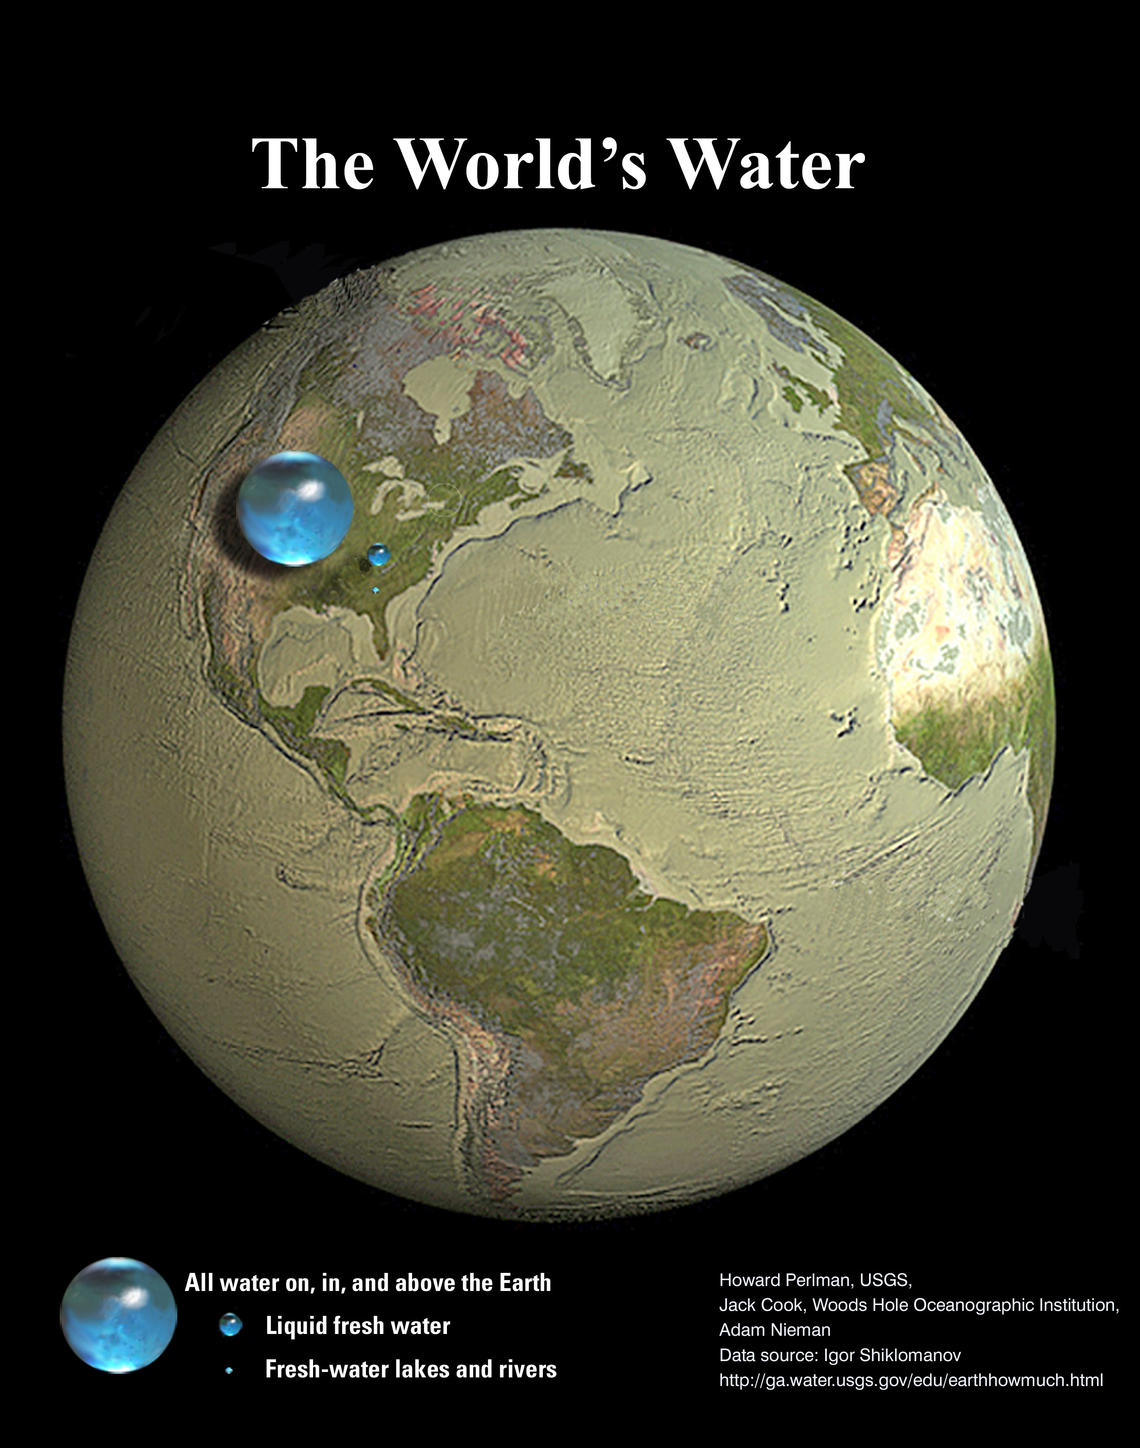
\includegraphics{archive/figures/all-the-worlds-water.jpg}

}

\caption{Source: Water Science School (2019c)}

\end{figure}

\begin{figure}

{\centering 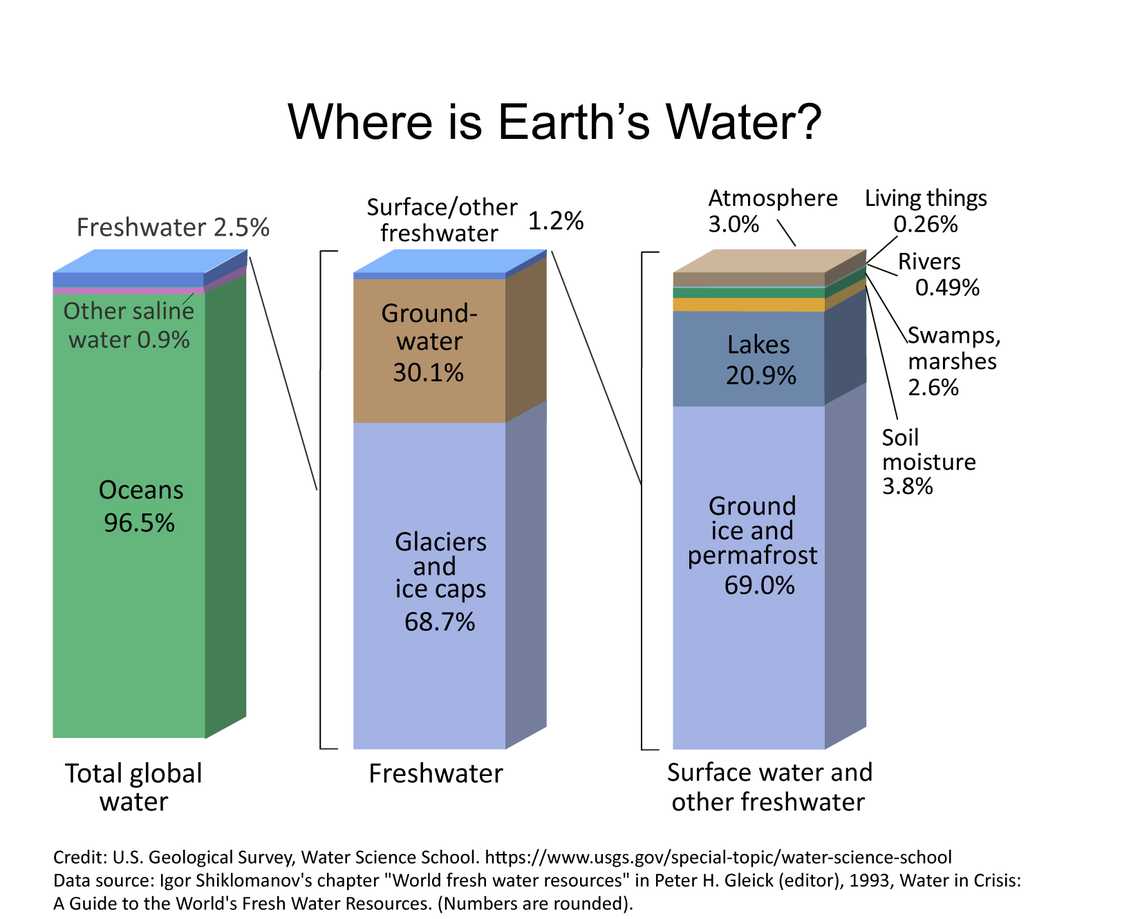
\includegraphics{archive/figures/EarthsWater-BarChart.png}

}

\caption{Source: Water Science School (2018)}

\end{figure}

\hypertarget{the-natural-water-cycle-2019}{%
\section{The natural water cycle
(2019)}\label{the-natural-water-cycle-2019}}

\begin{figure}

{\centering 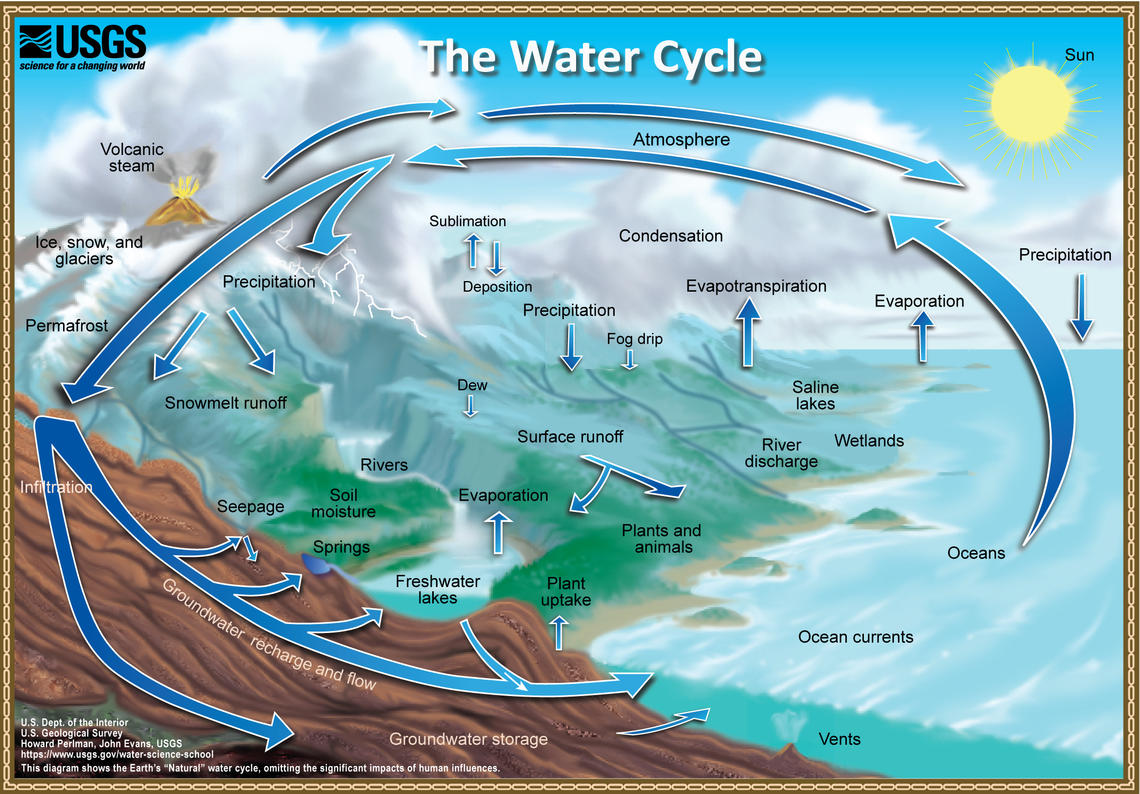
\includegraphics{archive/figures/water-cycle.jpg}

}

\caption{Source: Water Science School (2019g)}

\end{figure}

\hypertarget{the-new-water-cycle-2022}{%
\section{The new water cycle (2022)}\label{the-new-water-cycle-2022}}

\begin{figure}

{\centering \includegraphics{archive/figures/water-cycle-2022.png}

}

\caption{Source: Water Science School (2022)}

\end{figure}

Interactive chart:
\href{https://labs.waterdata.usgs.gov/visualizations/pools-and-fluxes/index.html}{Pools
and fluxes in the water cycle}

\hypertarget{global-water-distribution}{%
\section{Global water distribution}\label{global-water-distribution}}

\begin{longtable}[]{@{}
  >{\raggedright\arraybackslash}p{(\columnwidth - 6\tabcolsep) * \real{0.3000}}
  >{\raggedright\arraybackslash}p{(\columnwidth - 6\tabcolsep) * \real{0.3000}}
  >{\raggedright\arraybackslash}p{(\columnwidth - 6\tabcolsep) * \real{0.1500}}
  >{\raggedright\arraybackslash}p{(\columnwidth - 6\tabcolsep) * \real{0.1500}}@{}}
\caption{Source: Water Science School (2018). \textbf{(Percents are
rounded, so will not add to 100)}}\tabularnewline
\toprule()
\begin{minipage}[b]{\linewidth}\raggedright
Water source
\end{minipage} & \begin{minipage}[b]{\linewidth}\raggedright
Volume (km\(^3\))
\end{minipage} & \begin{minipage}[b]{\linewidth}\raggedright
\% of freshwater
\end{minipage} & \begin{minipage}[b]{\linewidth}\raggedright
\% of total water
\end{minipage} \\
\midrule()
\endfirsthead
\toprule()
\begin{minipage}[b]{\linewidth}\raggedright
Water source
\end{minipage} & \begin{minipage}[b]{\linewidth}\raggedright
Volume (km\(^3\))
\end{minipage} & \begin{minipage}[b]{\linewidth}\raggedright
\% of freshwater
\end{minipage} & \begin{minipage}[b]{\linewidth}\raggedright
\% of total water
\end{minipage} \\
\midrule()
\endhead
Oceans, Seas, \& Bays & 1,338,000,000 & -- & 96.54 \\
Ice caps, Glaciers, \& Permanent Snow & 24,064,000 & 68.7 & 1.74 \\
Groundwater & 23,400,000 & -- & 1.69 \\
\(\quad\)Fresh & 10,530,000 & 30.1 & 0.76 \\
\(\quad\)Saline & 12,870,000 & -- & 0.93 \\
Soil Moisture & 16,500 & 0.05 & 0.001 \\
Ground Ice \& Permafrost & 300,000 & 0.86 & 0.022 \\
Lakes & 176,400 & -- & 0.013 \\
\(\quad\)Fresh & 91,000 & 0.26 & 0.007 \\
\(\quad\)Saline & 85,400 & -- & 0.006 \\
Atmosphere & 12,900 & 0.04 & 0.001 \\
Swamp Water & 11,470 & 0.03 & 0.0008 \\
Rivers & 2,120 & 0.006 & 0.0002 \\
Biological Water & 1,120 & 0.003 & 0.0001 \\
\bottomrule()
\end{longtable}

\hypertarget{energy-drives-the-hydrologic-cycle}{%
\section{Energy drives the hydrologic
cycle}\label{energy-drives-the-hydrologic-cycle}}

From Margulis (2019)

\begin{quote}
A key aspect of the hydrologic cycle is the fact that it is driven by
energy inputs (primarily from the sun). At the global scale, the system
is essentially closed with respect to water; negligible water is
entering or leaving the system. In other words, there is no external
forcing in terms of a water flux. Systems with no external forcing will
generally eventually come to an equilibrium state. So what makes the
hydrologic cycle so dynamic? The solar radiative energy input, which is
external to the system, drives the hydrologic cycle. Averaged over the
globe, 342 W m\(^{-2}\) of solar radiative energy is being continuously
input to the system at the top of the atmosphere. This energy input must
be dissipated, and this is done, to a large extent, via the hydrologic
cycle. Due to this fact, the study of hydrology is not isolated to the
study of water storage and movement, but also must often include study
of energy storage and movements.
\end{quote}

\hypertarget{components-of-the-water-cycle}{%
\section{Components of the water
cycle}\label{components-of-the-water-cycle}}

\hypertarget{water-storage-in-oceans}{%
\subsection{Water storage in oceans}\label{water-storage-in-oceans}}

\hypertarget{evaporation-sublimation}{%
\subsection{Evaporation / Sublimation}\label{evaporation-sublimation}}

Evaporation \(\longrightarrow\) cooling

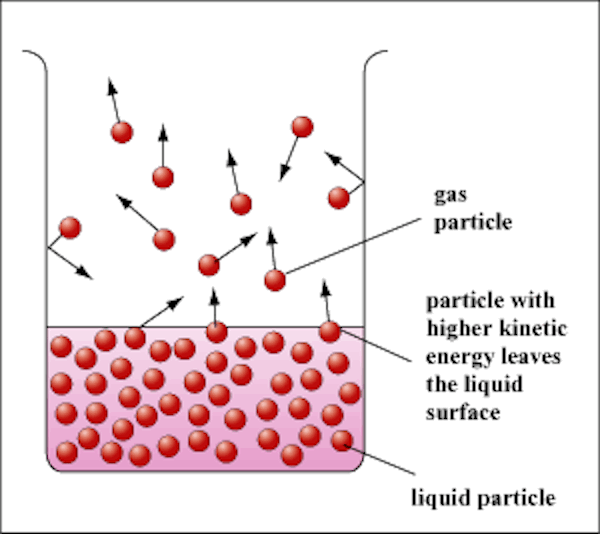
\includegraphics{archive/figures/evaporation_1.gif}

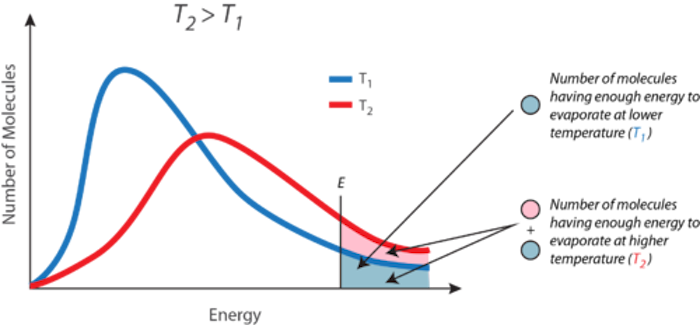
\includegraphics{archive/figures/evaporation_2.png}

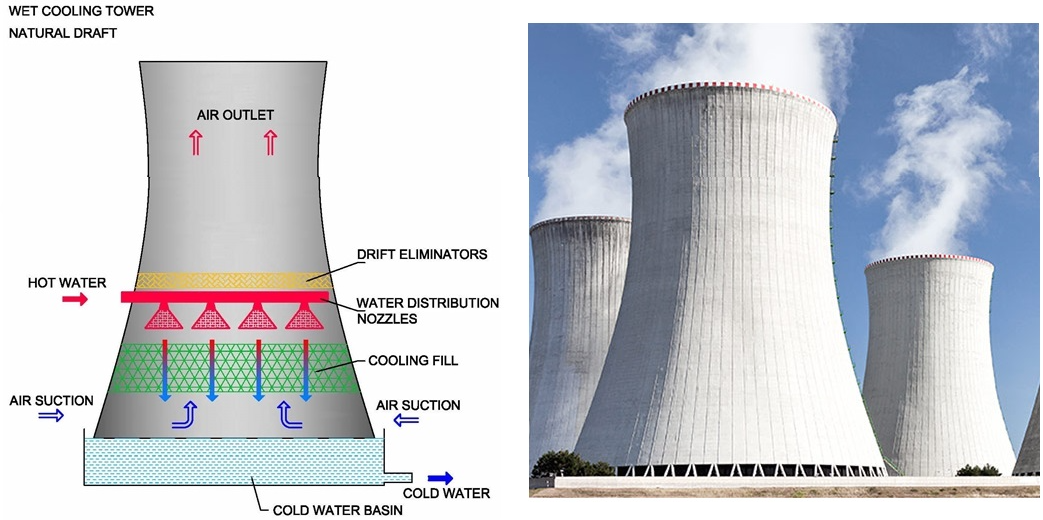
\includegraphics{archive/figures/cooling-tower.png}

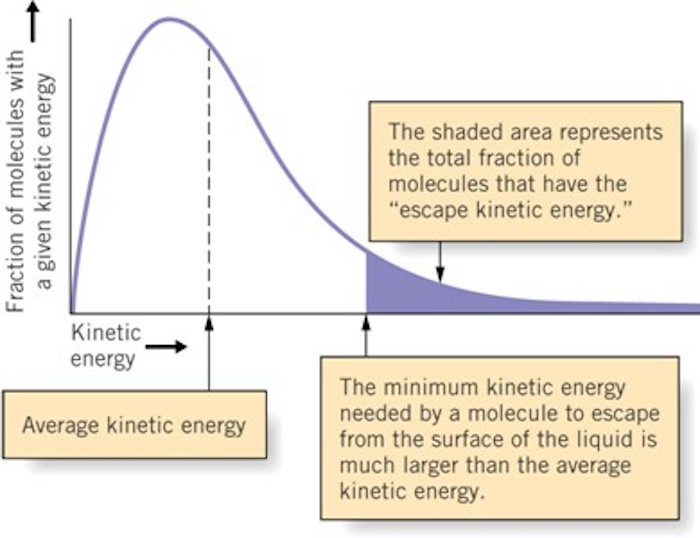
\includegraphics{archive/figures/evaporation_slide0.jpg}
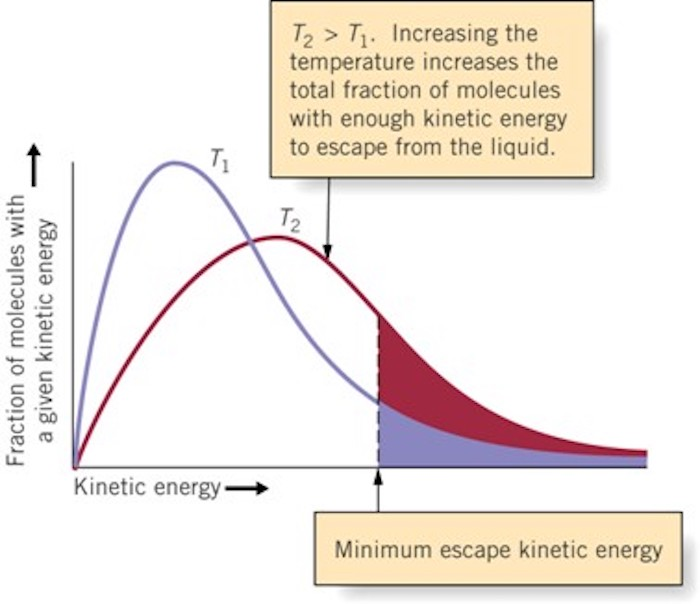
\includegraphics{archive/figures/evaporation_slide1.jpg}
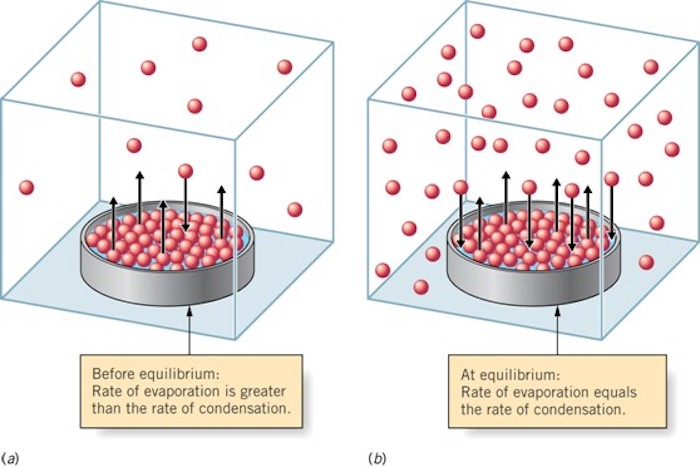
\includegraphics{archive/figures/evaporation_slide2.jpg}

\hypertarget{evapotranspiration}{%
\subsection{Evapotranspiration}\label{evapotranspiration}}

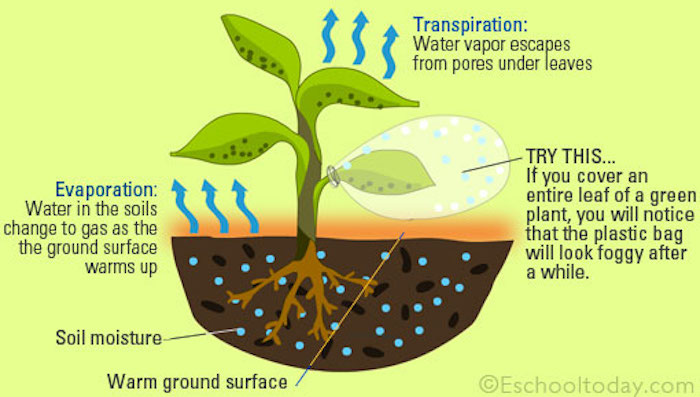
\includegraphics{archive/figures/evapotranspiration1.jpg}

\hypertarget{water-storage-in-the-atmosphere}{%
\subsection{Water storage in the
atmosphere}\label{water-storage-in-the-atmosphere}}

Cumulonimbus cloud over Africa
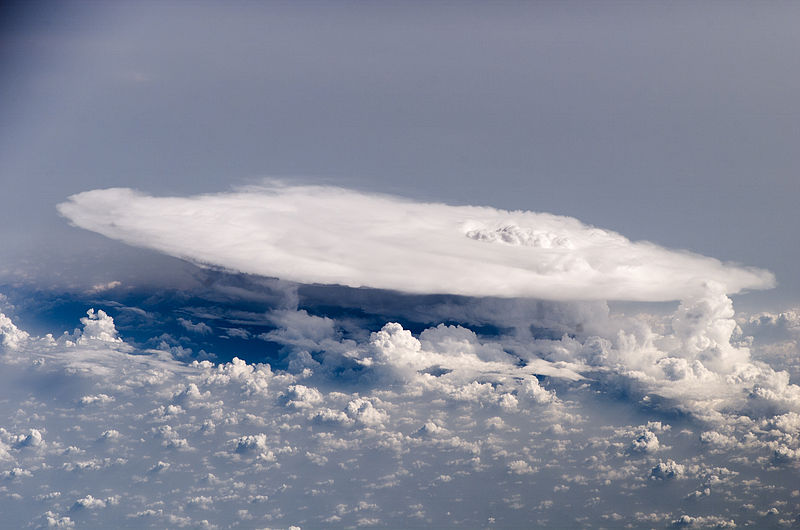
\includegraphics{archive/figures/cumulonimbus.jpg}

Picture of cumulonimbus taken from the International Space Station, over
western Africa near the Senegal-Mali border.

If all of the water in the atmosphere rained down at once, it would only
cover the globe to a depth of 2.5 centimeters. \[
\begin{align}
\text{amount of water in the atmosphere} & \qquad V = 12\, 900\, \text{km}^3 \\
\text{surface of Earth} & \qquad S = 4 \pi R^2;\quad R=6371\,\text{km}\\
& \qquad V = S \times h \\
\text{height} & \qquad h = \frac{V}{S} \simeq 2.5\,\text{cm}
\end{align}
\]

Try to calculate this yourself, and click on the button below to check
how to do it.

\begin{Shaded}
\begin{Highlighting}[]
\CommentTok{\# amount of water in the atmosphere}
\NormalTok{V }\OperatorTok{=} \DecValTok{12900} \CommentTok{\# km\^{}3}
\CommentTok{\# Earth\textquotesingle{}s radius}
\NormalTok{R }\OperatorTok{=} \DecValTok{6371} \CommentTok{\# km}
\CommentTok{\# surface of Earth = 4 pi Rˆ2}
\NormalTok{S }\OperatorTok{=} \DecValTok{4} \OperatorTok{*} \FloatTok{3.141592} \OperatorTok{*}\NormalTok{ R}\OperatorTok{**}\DecValTok{2}
\CommentTok{\# Volume: V = S * h, therefore}
\CommentTok{\# height}
\NormalTok{h }\OperatorTok{=}\NormalTok{ V }\OperatorTok{/}\NormalTok{ S }\CommentTok{\# in km}
\NormalTok{h\_cm }\OperatorTok{=}\NormalTok{ h }\OperatorTok{*} \FloatTok{1e5} \CommentTok{\# in cm}
\BuiltInTok{print}\NormalTok{(}\SpecialStringTok{f"The height would be \textasciitilde{} }\SpecialCharTok{\{}\NormalTok{h\_cm}\SpecialCharTok{:.1f\}}\SpecialStringTok{ cm"}\NormalTok{)}
\end{Highlighting}
\end{Shaded}

\begin{verbatim}
The height would be ~ 2.5 cm
\end{verbatim}

\hypertarget{condensation}{%
\subsection{Condensation}\label{condensation}}

\hypertarget{precipitation}{%
\subsection{Precipitation}\label{precipitation}}

\begin{figure}

{\centering 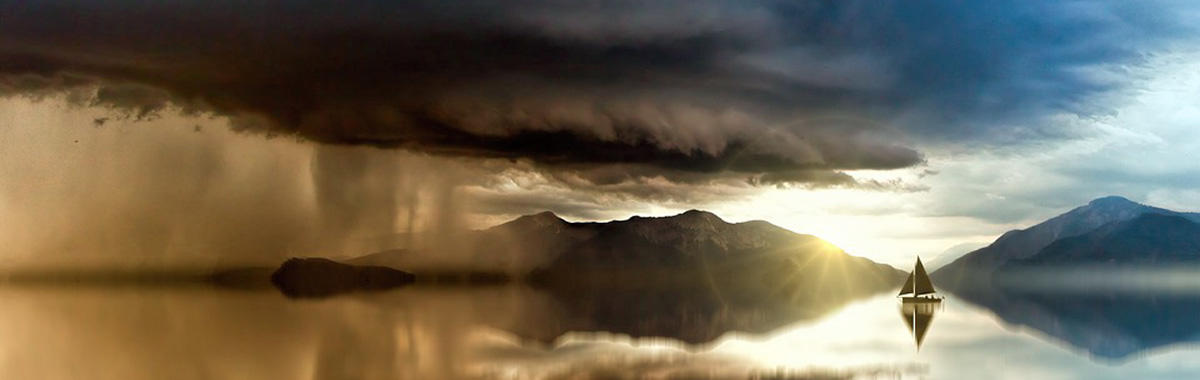
\includegraphics{archive/figures/rain-burst1.jpg}

}

\caption{Source: Water Science School (2019f)}

\end{figure}

\begin{longtable}[]{@{}
  >{\raggedright\arraybackslash}p{(\columnwidth - 8\tabcolsep) * \real{0.2800}}
  >{\raggedright\arraybackslash}p{(\columnwidth - 8\tabcolsep) * \real{0.1800}}
  >{\raggedright\arraybackslash}p{(\columnwidth - 8\tabcolsep) * \real{0.1800}}
  >{\raggedright\arraybackslash}p{(\columnwidth - 8\tabcolsep) * \real{0.1800}}
  >{\raggedright\arraybackslash}p{(\columnwidth - 8\tabcolsep) * \real{0.1800}}@{}}
\caption{Source: Water Science School (2019e)}\tabularnewline
\toprule()
\begin{minipage}[b]{\linewidth}\raggedright
\end{minipage} & \begin{minipage}[b]{\linewidth}\raggedright
Intensity (cm/h)
\end{minipage} & \begin{minipage}[b]{\linewidth}\raggedright
Median diameter (mm)
\end{minipage} & \begin{minipage}[b]{\linewidth}\raggedright
Velocity of fall (m/s)
\end{minipage} & \begin{minipage}[b]{\linewidth}\raggedright
Drops s\(^{-1}\) m\(^{-2}\)
\end{minipage} \\
\midrule()
\endfirsthead
\toprule()
\begin{minipage}[b]{\linewidth}\raggedright
\end{minipage} & \begin{minipage}[b]{\linewidth}\raggedright
Intensity (cm/h)
\end{minipage} & \begin{minipage}[b]{\linewidth}\raggedright
Median diameter (mm)
\end{minipage} & \begin{minipage}[b]{\linewidth}\raggedright
Velocity of fall (m/s)
\end{minipage} & \begin{minipage}[b]{\linewidth}\raggedright
Drops s\(^{-1}\) m\(^{-2}\)
\end{minipage} \\
\midrule()
\endhead
Fog & 0.013 & 0.01 & 0.003 & 67,425,000 \\
Mist & 0.005 & 0.1 & 0.21 & 27,000 \\
Drizzle & 0.025 & 0.96 & 4.1 & 151 \\
Light rain & 0.10 & 1.24 & 4.8 & 280 \\
Moderate rain & 0.38 & 1.60 & 5.7 & 495 \\
Heavy rain & 1.52 & 2.05 & 6.7 & 495 \\
Excessive rain & 4.06 & 2.40 & 7.3 & 818 \\
Cloudburst & 10.2 & 2.85 & 7.9 & 1,220 \\
\bottomrule()
\end{longtable}

\hypertarget{water-storage-in-ice-and-snow}{%
\subsection{Water storage in ice and
snow}\label{water-storage-in-ice-and-snow}}

\begin{figure}

{\centering 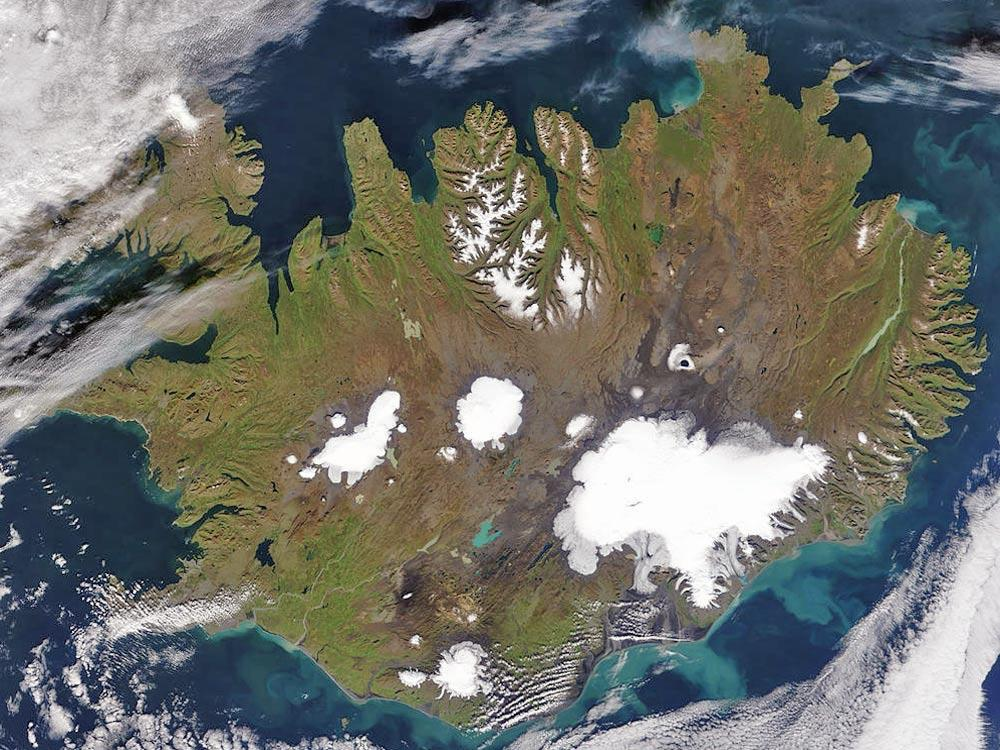
\includegraphics{archive/figures/iceland-summer.jpg}

}

\caption{Source: Water Science School (2019d)}

\end{figure}

\begin{figure}

{\centering 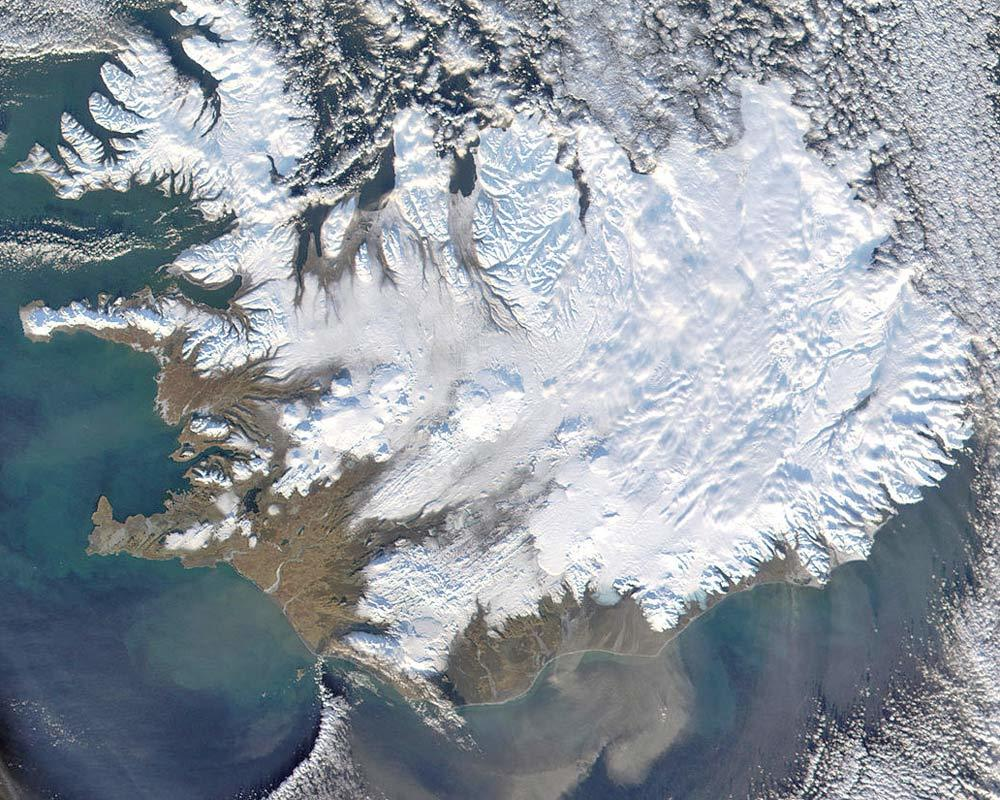
\includegraphics{archive/figures/iceland-winter.jpg}

}

\caption{Source: Water Science School (2019d)}

\end{figure}

\hypertarget{snowmelt-runoff-to-streams}{%
\subsection{Snowmelt runoff to
streams}\label{snowmelt-runoff-to-streams}}

\hypertarget{surface-runoff}{%
\subsection{Surface runoff}\label{surface-runoff}}

\begin{figure}

{\centering 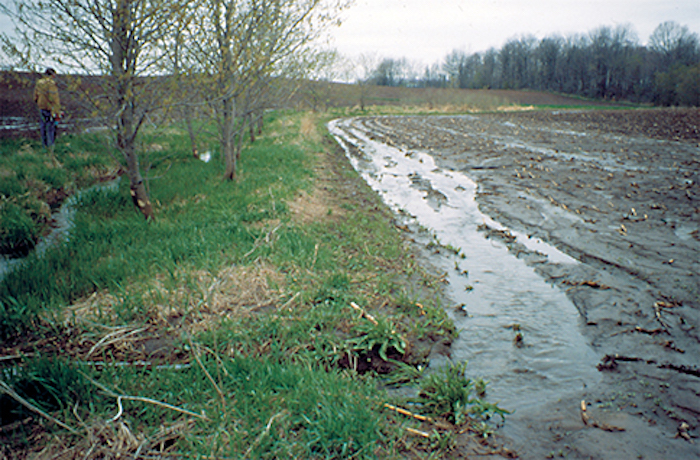
\includegraphics{archive/figures/runoff-field.jpg}

}

\caption{Source: חדשות פתח תקווה (2020)}

\end{figure}

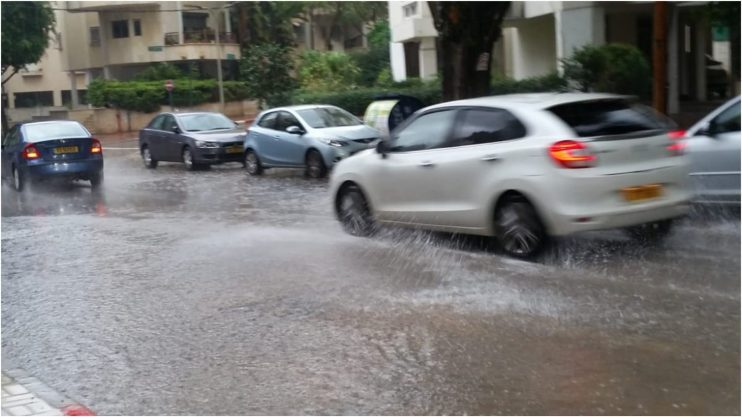
\includegraphics{archive/figures/runoff-city.jpg}

\hypertarget{streamflow}{%
\subsection{Streamflow}\label{streamflow}}

The Mississippi river basin is very large
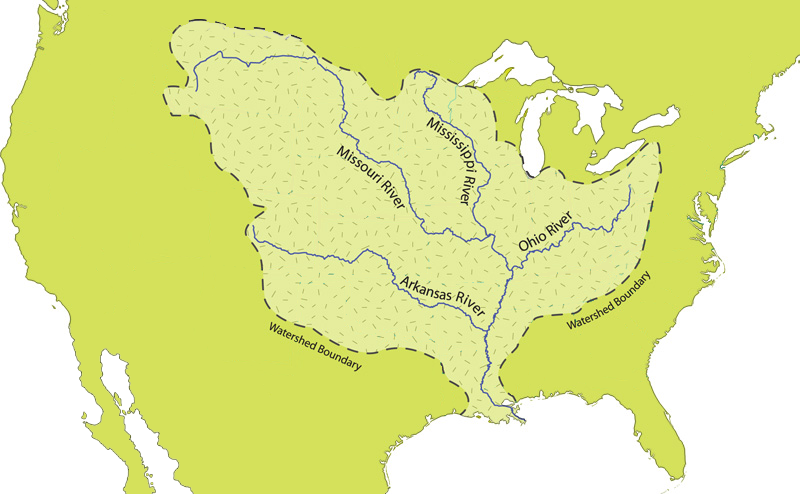
\includegraphics{archive/figures/Mississippi_River_Watershed_Map_North_America.png}

The Amazon river basin is \textbf{Huge}
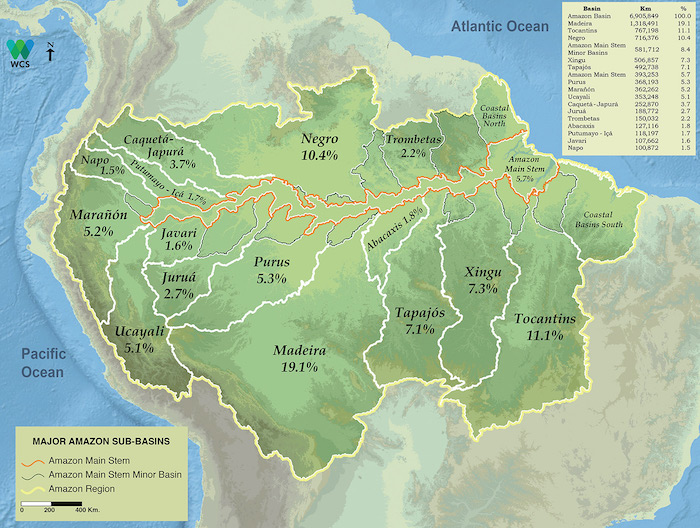
\includegraphics{archive/figures/amazon-basin.jpg}

\begin{figure}

{\centering 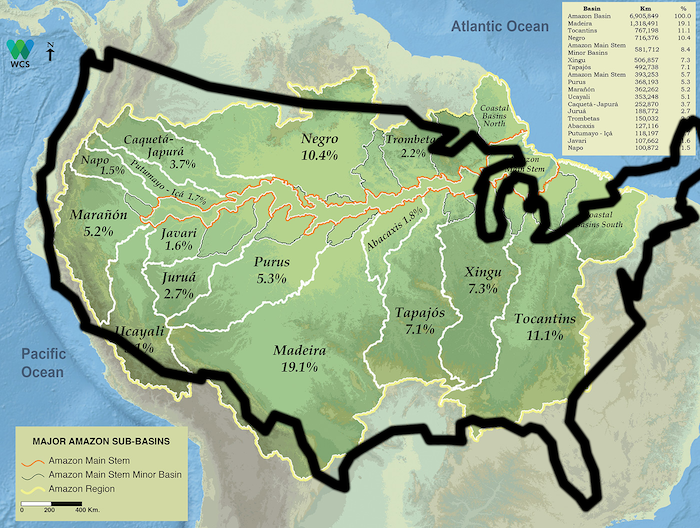
\includegraphics{archive/figures/amazon-basin-us.png}

}

\caption{Source: Yair Mau}

\end{figure}

\hypertarget{lakes-and-rivers}{%
\subsection{Lakes and rivers}\label{lakes-and-rivers}}

\begin{figure}

{\centering 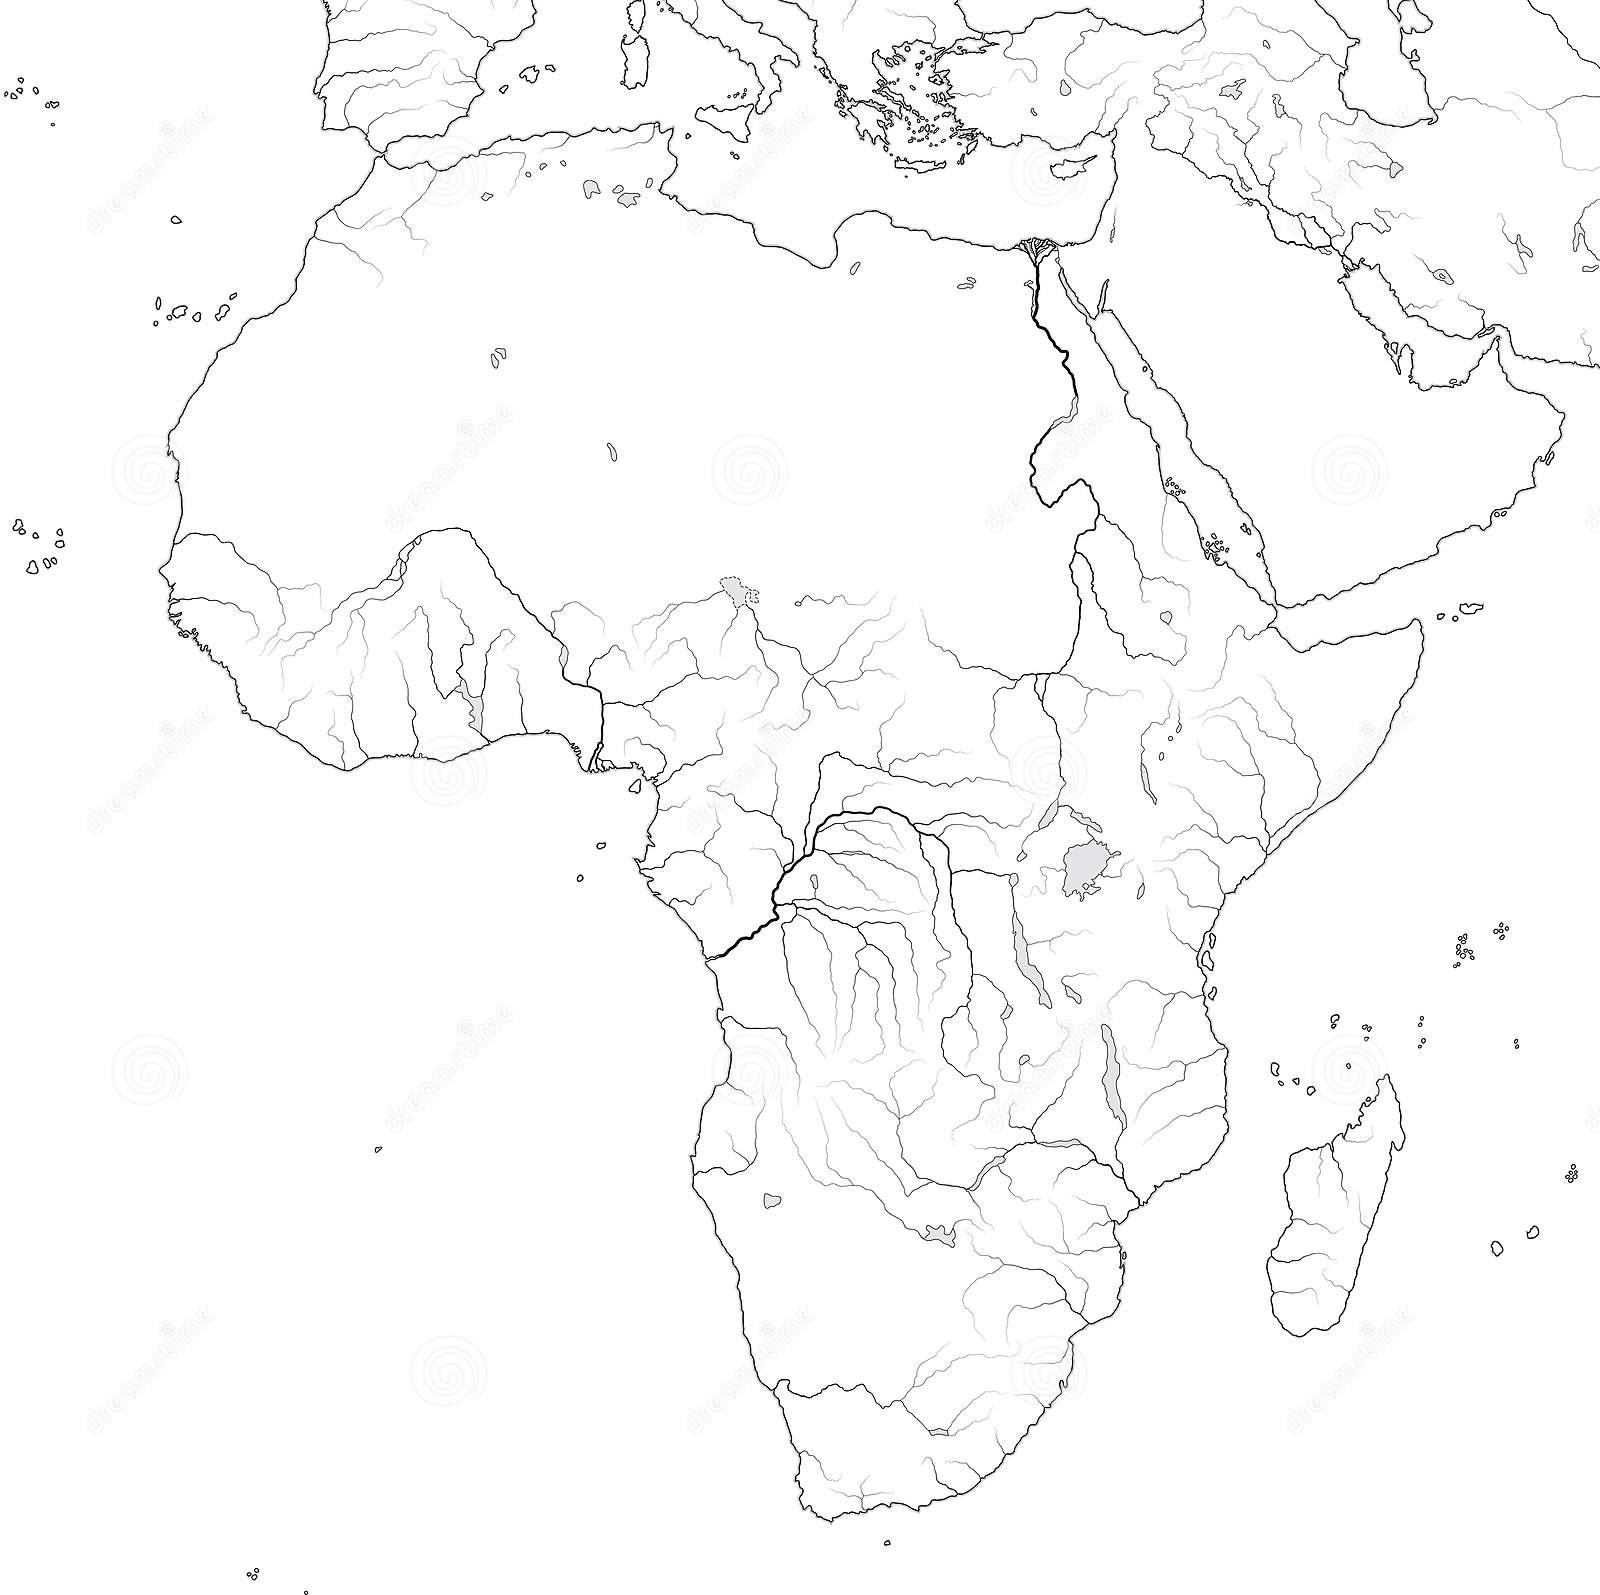
\includegraphics{archive/figures/rivers-africa.png}

}

\caption{Source: dreamstime (2022)}

\end{figure}

Lake Malawi 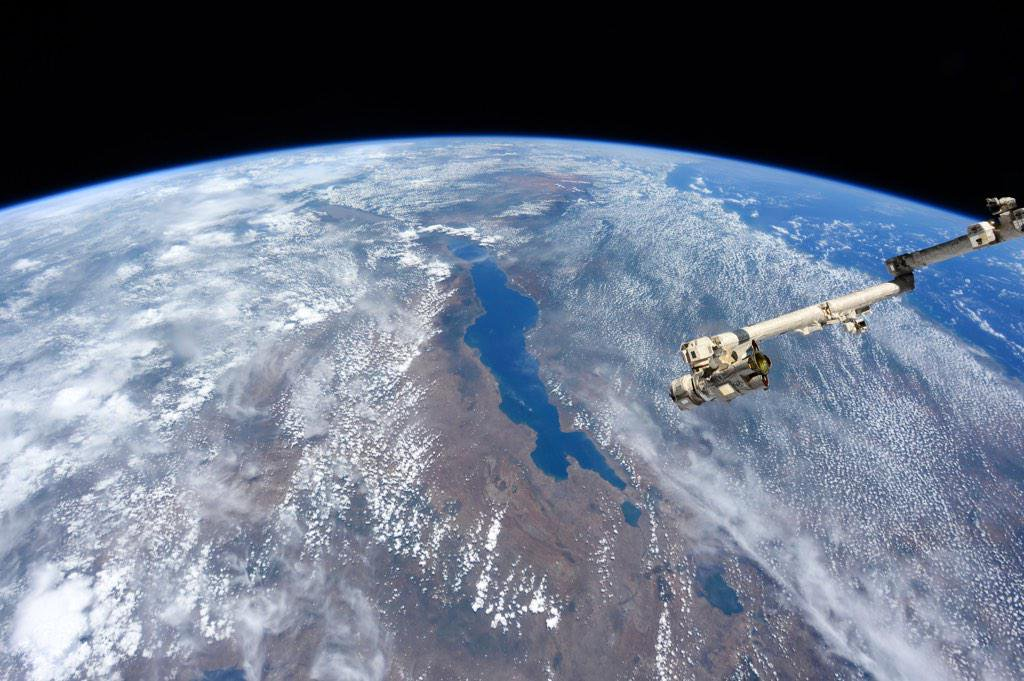
\includegraphics{archive/figures/lake-malawi.jpg}

\begin{figure}

{\centering 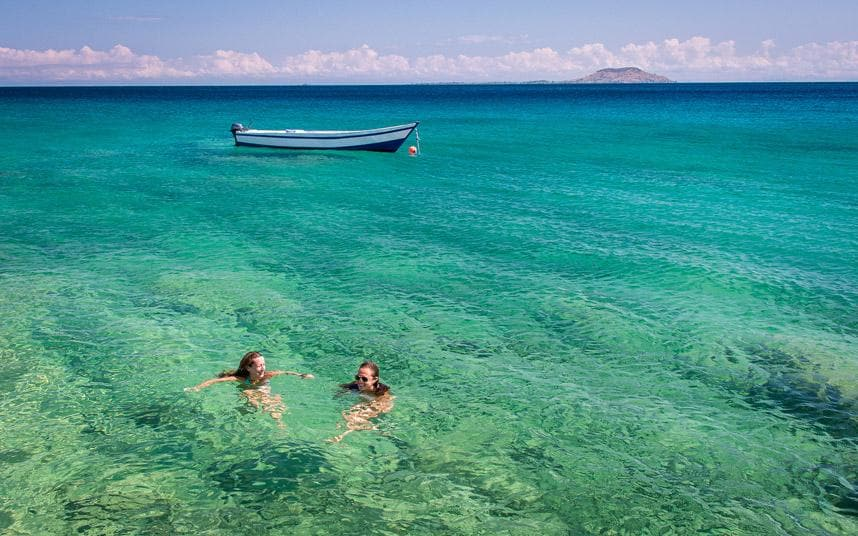
\includegraphics{archive/figures/lake-malawi2.jpg}

}

\caption{Source: Fiona Bruce (2015)}

\end{figure}

\hypertarget{infiltration}{%
\subsection{Infiltration}\label{infiltration}}

\begin{figure}

{\centering 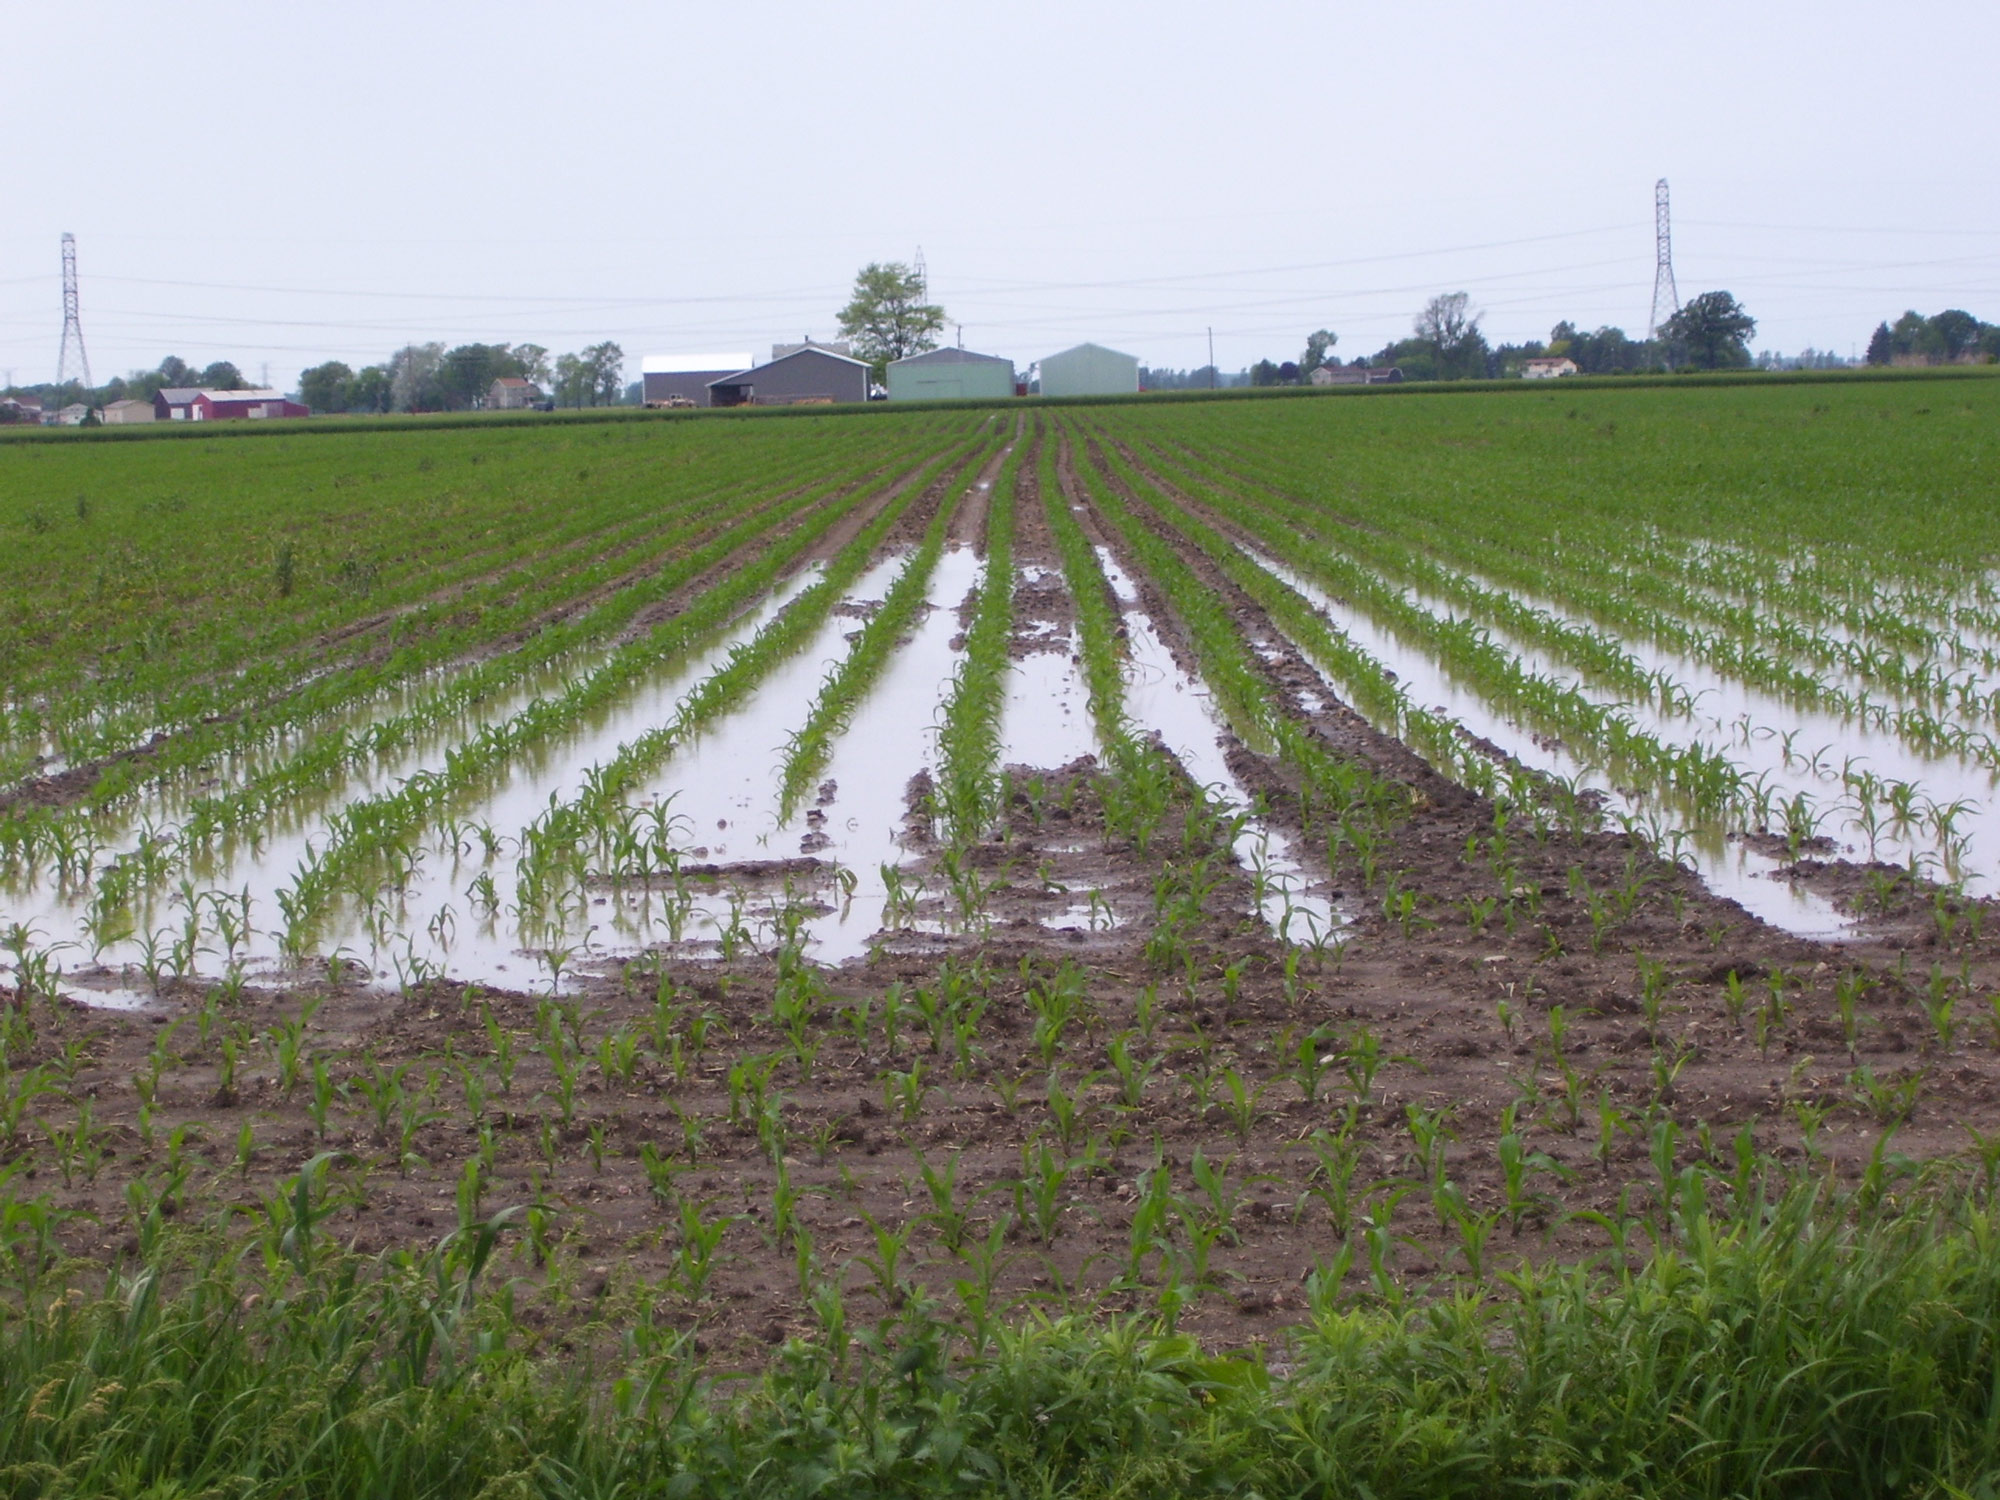
\includegraphics{archive/figures/infiltration.jpg}

}

\caption{Source: Suma Groulx (2015)}

\end{figure}

\hypertarget{groundwater-storage}{%
\subsection{Groundwater storage}\label{groundwater-storage}}

\begin{figure}

{\centering 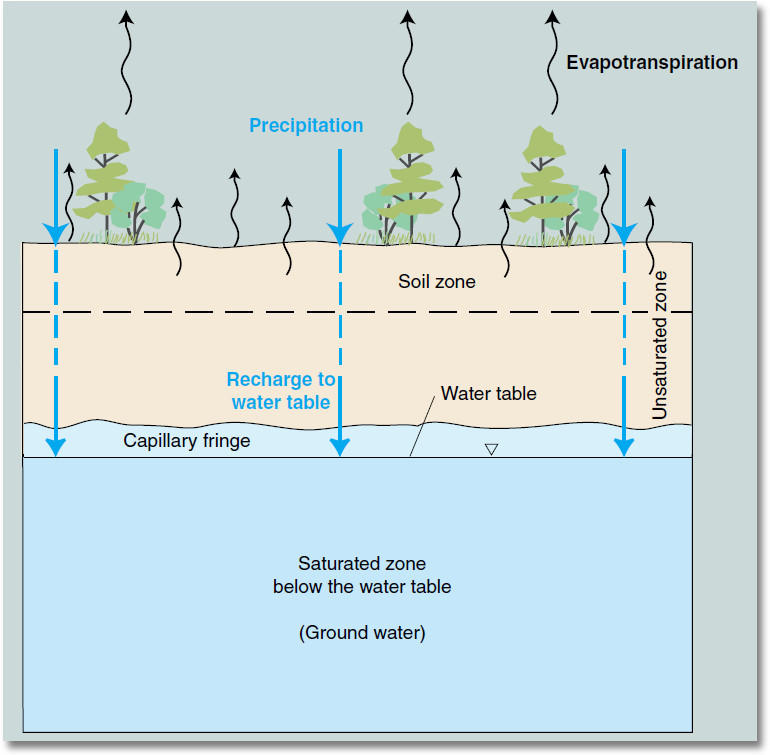
\includegraphics{archive/figures/groundwater.jpg}

}

\caption{Source: Water Science School (2019b)}

\end{figure}

\begin{figure}

{\centering 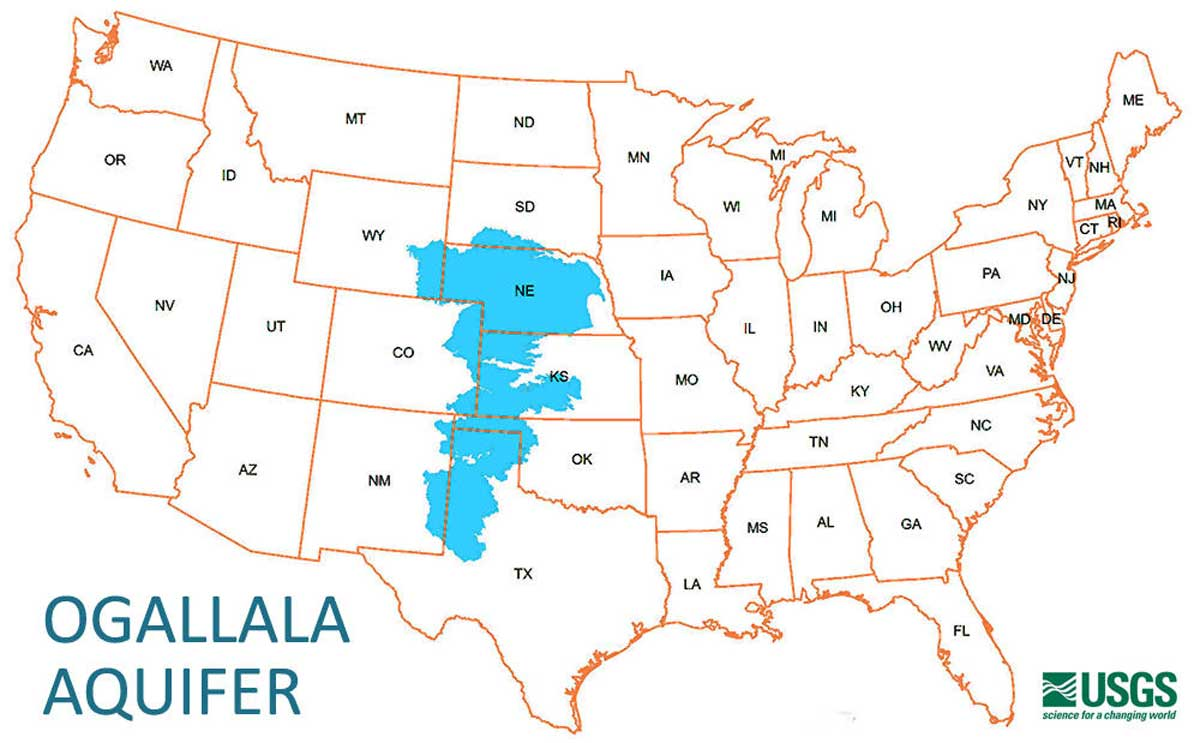
\includegraphics{archive/figures/ogallala_aquifer_usgs.jpg}

}

\caption{Source: (\textbf{modernfarmer?})}

\end{figure}

\begin{figure}

{\centering 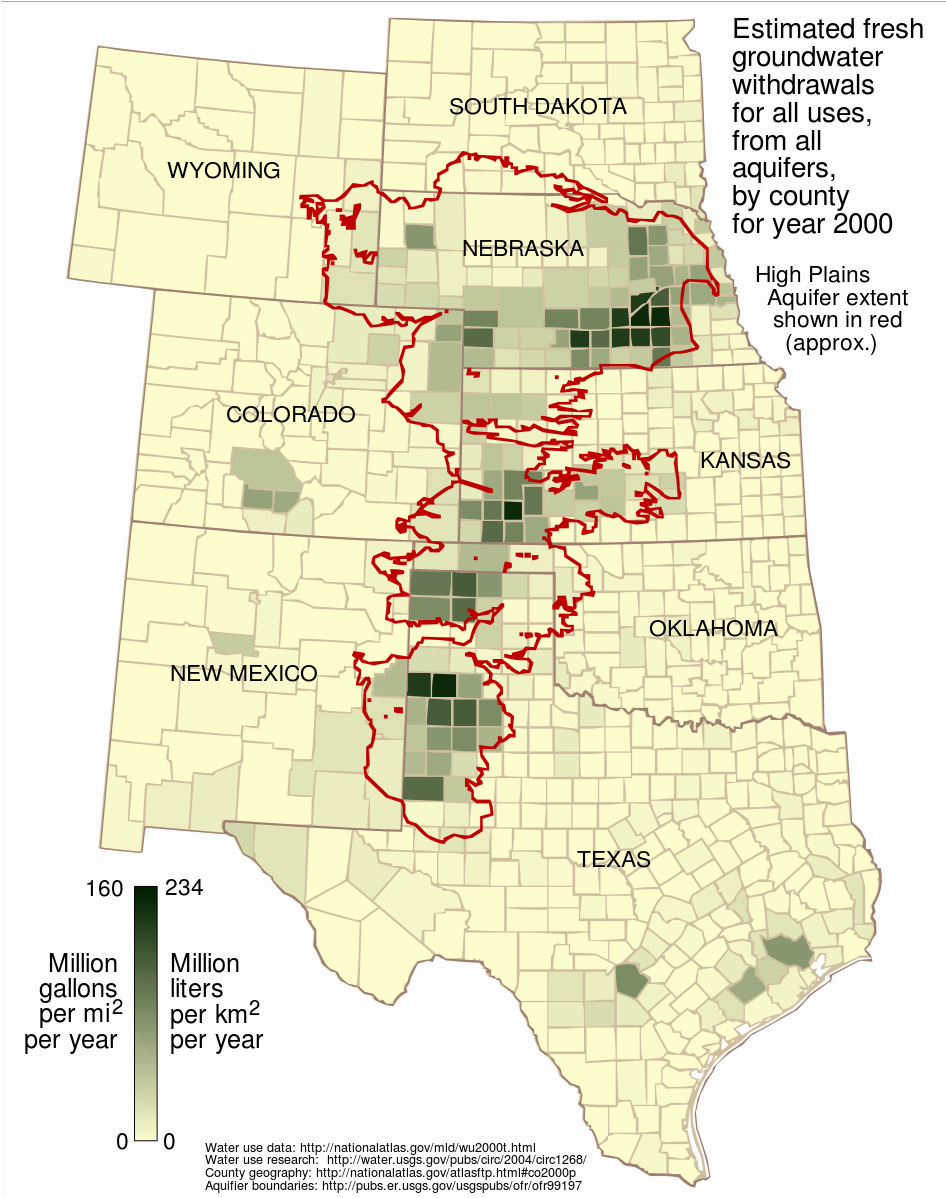
\includegraphics{archive/figures/ogallala_aquifer_wiki.png}

}

\caption{Source: (\textbf{ogallala1?})}

\end{figure}

Center Pivot irrigation in Nebraska taps the Ogallala Aquifer.
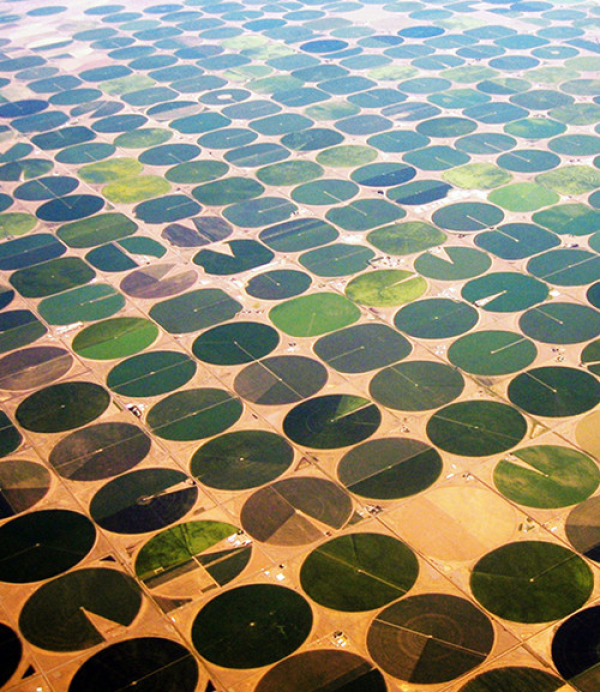
\includegraphics{archive/figures/groundwater-ogallala-aquifer.jpg}

\hypertarget{groundwater-flow-and-discharge}{%
\subsection{Groundwater flow and
discharge}\label{groundwater-flow-and-discharge}}

\begin{figure}

{\centering 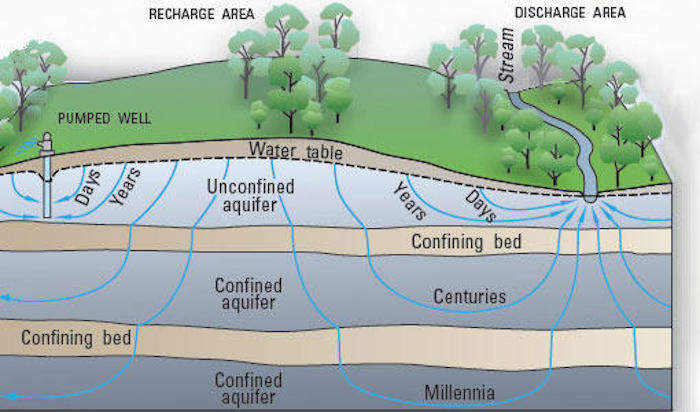
\includegraphics{archive/figures/groundwater-flow-diagram.jpg}

}

\caption{Source: Water Science School (2019a)}

\end{figure}

\begin{figure}

{\centering 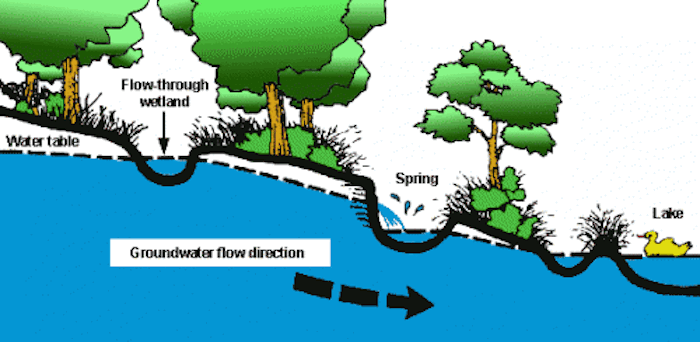
\includegraphics{archive/figures/groundwater-discharge.gif}

}

\caption{Source: Raymond, Lyle S. Jr. (1988)}

\end{figure}

\begin{figure}

{\centering 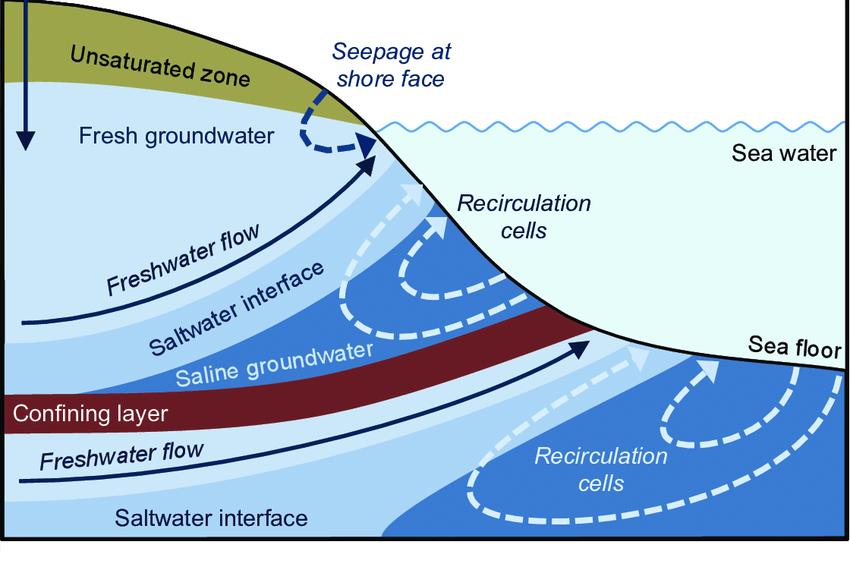
\includegraphics{archive/figures/groundwater-discharge-submarine.png}

}

\caption{Source: Valentí Rodellas (1988)}

\end{figure}

\hypertarget{spring}{%
\subsection{Spring}\label{spring}}

Ein Gedi 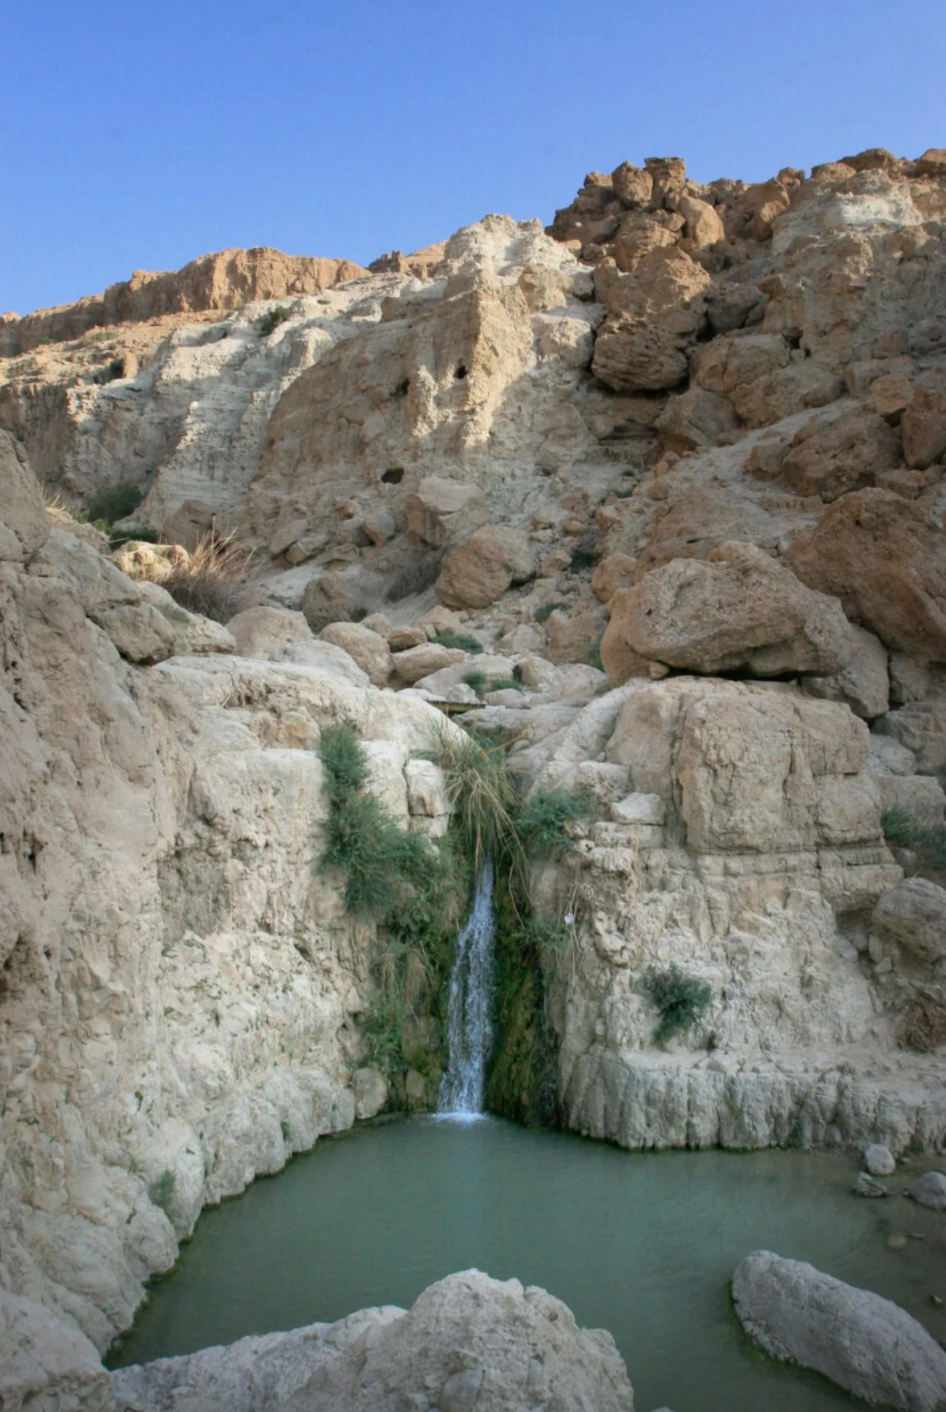
\includegraphics{archive/figures/spring-ein-gedi.png}

Thousand Springs, Idaho
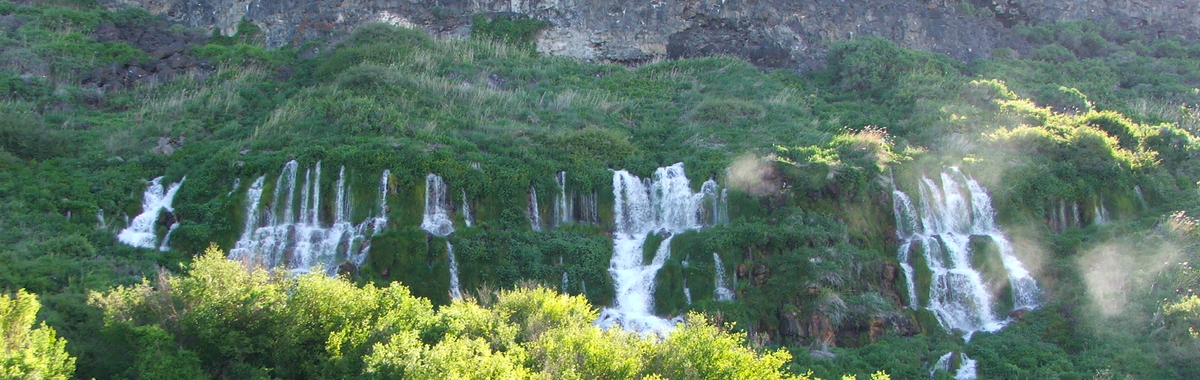
\includegraphics{archive/figures/spring-Thousand-Springs-Idaho.png}

\hypertarget{exercises}{%
\chapter{Exercises}\label{exercises}}

\textbf{let's have fun plotting some data 😀}

\hypertarget{download-the-data}{%
\section{download the data}\label{download-the-data}}

\begin{enumerate}
\def\labelenumi{\arabic{enumi}.}
\tightlist
\item
  Go to the Faculty of Agriculture's
  \href{http://www.meteo-tech.co.il/faculty/faculty.asp?client=1}{weather
  station}.
\item
  Click on משיכת נתונים and download data for 1 September 2020 to 28
  February 2021, with a 24h interval. Call it
  \texttt{data-sep2020-feb2021}
\item
  Open the .csv file with Excel, see how it looks like
\item
  If you can't download the data, just click
  \href{/archive/data/data-sep2020-feb2021.csv}{here}.
\end{enumerate}

\hypertarget{import-packages}{%
\section{import packages}\label{import-packages}}

We need to import this data into python. First we import useful
packages. \textbf{Type} (don't copy and paste) the following lines in
the code cell below.

\begin{Shaded}
\begin{Highlighting}[]
\ImportTok{import}\NormalTok{ pandas }\ImportTok{as}\NormalTok{ pd}
\ImportTok{import}\NormalTok{ numpy }\ImportTok{as}\NormalTok{ np}
\ImportTok{import}\NormalTok{ matplotlib.pyplot }\ImportTok{as}\NormalTok{ plt}
\ImportTok{import}\NormalTok{ seaborn }\ImportTok{as}\NormalTok{ sns}
\NormalTok{sns.}\BuiltInTok{set}\NormalTok{(style}\OperatorTok{=}\StringTok{"ticks"}\NormalTok{, font\_scale}\OperatorTok{=}\FloatTok{1.5}\NormalTok{)}
\end{Highlighting}
\end{Shaded}

\hypertarget{import-data-with-pandas}{%
\section{import data with pandas}\label{import-data-with-pandas}}

Import data from csv and put it in a pandas \textbf{dataframe} (a
table). Make line 5 the header (column names)

\begin{Shaded}
\begin{Highlighting}[]
\NormalTok{df }\OperatorTok{=}\NormalTok{ pd.read\_csv(}\StringTok{"data{-}sep2020{-}feb2021.csv"}\NormalTok{, header}\OperatorTok{=}\NormalTok{[}\DecValTok{4}\NormalTok{])}
\NormalTok{df}
\end{Highlighting}
\end{Shaded}

\begin{longtable}[]{@{}lllllll@{}}
\toprule()
& Unnamed: 0 & �C & �C.1 & km/h & mm & mm.1 \\
\midrule()
\endhead
0 & 01/09/20 & 32.8 & 25.3 & 29.7 & 0.0 & 0.0 \\
1 & 02/09/20 & 33.0 & 24.0 & 28.8 & 0.0 & 0.0 \\
2 & 03/09/20 & 34.2 & 23.8 & 31.6 & 0.0 & 0.0 \\
3 & 04/09/20 & 36.3 & 27.3 & 24.2 & 0.0 & 0.0 \\
4 & 05/09/20 & 34.2 & 26.3 & 22.4 & 0.0 & 0.0 \\
... & ... & ... & ... & ... & ... & ... \\
176 & 24/02/21 & 20.6 & 9.9 & 28.8 & 0.0 & 481.7 \\
177 & 25/02/21 & 19.4 & 9.3 & 23.3 & 0.0 & 481.7 \\
178 & 26/02/21 & 21.3 & 8.0 & 24.2 & 0.1 & 481.8 \\
179 & 27/02/21 & 23.4 & 9.2 & 30.6 & 0.0 & 481.8 \\
180 & 28/02/21 & 19.7 & 9.2 & 22.4 & 0.0 & 481.8 \\
\bottomrule()
\end{longtable}

\hypertarget{rename-columns}{%
\section{rename columns}\label{rename-columns}}

rename the columns to:\\
\texttt{date,\ tmax,\ tmin,\ wind,\ rain24h,\ rain\_cumulative}

\begin{Shaded}
\begin{Highlighting}[]
\NormalTok{df.columns }\OperatorTok{=}\NormalTok{ [}\StringTok{\textquotesingle{}date\textquotesingle{}}\NormalTok{, }\StringTok{\textquotesingle{}tmax\textquotesingle{}}\NormalTok{, }\StringTok{\textquotesingle{}tmin\textquotesingle{}}\NormalTok{, }\StringTok{\textquotesingle{}wind\textquotesingle{}}\NormalTok{, }\StringTok{\textquotesingle{}rain24h\textquotesingle{}}\NormalTok{, }\StringTok{\textquotesingle{}rain\_cumulative\textquotesingle{}}\NormalTok{]}
\NormalTok{df}
\end{Highlighting}
\end{Shaded}

\begin{longtable}[]{@{}lllllll@{}}
\toprule()
& date & tmax & tmin & wind & rain24h & rain\_cumulative \\
\midrule()
\endhead
0 & 01/09/20 & 32.8 & 25.3 & 29.7 & 0.0 & 0.0 \\
1 & 02/09/20 & 33.0 & 24.0 & 28.8 & 0.0 & 0.0 \\
2 & 03/09/20 & 34.2 & 23.8 & 31.6 & 0.0 & 0.0 \\
3 & 04/09/20 & 36.3 & 27.3 & 24.2 & 0.0 & 0.0 \\
4 & 05/09/20 & 34.2 & 26.3 & 22.4 & 0.0 & 0.0 \\
... & ... & ... & ... & ... & ... & ... \\
176 & 24/02/21 & 20.6 & 9.9 & 28.8 & 0.0 & 481.7 \\
177 & 25/02/21 & 19.4 & 9.3 & 23.3 & 0.0 & 481.7 \\
178 & 26/02/21 & 21.3 & 8.0 & 24.2 & 0.1 & 481.8 \\
179 & 27/02/21 & 23.4 & 9.2 & 30.6 & 0.0 & 481.8 \\
180 & 28/02/21 & 19.7 & 9.2 & 22.4 & 0.0 & 481.8 \\
\bottomrule()
\end{longtable}

\hypertarget{a-first-plot}{%
\section{a first plot!}\label{a-first-plot}}

plot the minimum temperature:

\begin{Shaded}
\begin{Highlighting}[]
\NormalTok{plt.plot(df[}\StringTok{\textquotesingle{}tmin\textquotesingle{}}\NormalTok{])}
\end{Highlighting}
\end{Shaded}

\begin{figure}[H]

{\centering 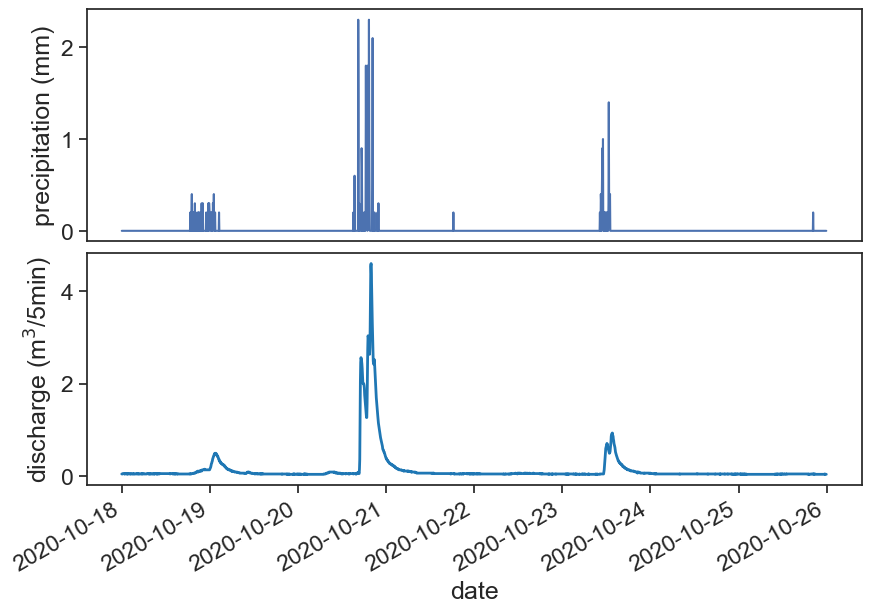
\includegraphics{introduction/introduction-exercises_files/figure-pdf/cell-5-output-1.png}

}

\end{figure}

\hypertarget{how-to-deal-with-dates}{%
\section{how to deal with dates}\label{how-to-deal-with-dates}}

We want the dates to appear on the horizontal axis.\\
Interpret `date' column as a pandas datetime, see how it looks different
from before\\
before: 01/09/20\\
after: 2020-09-01

\begin{Shaded}
\begin{Highlighting}[]
\NormalTok{df[}\StringTok{\textquotesingle{}date\textquotesingle{}}\NormalTok{] }\OperatorTok{=}\NormalTok{ pd.to\_datetime(df[}\StringTok{\textquotesingle{}date\textquotesingle{}}\NormalTok{], dayfirst}\OperatorTok{=}\VariableTok{True}\NormalTok{)}
\NormalTok{df}
\end{Highlighting}
\end{Shaded}

\begin{longtable}[]{@{}lllllll@{}}
\toprule()
& date & tmax & tmin & wind & rain24h & rain\_cumulative \\
\midrule()
\endhead
0 & 2020-09-01 & 32.8 & 25.3 & 29.7 & 0.0 & 0.0 \\
1 & 2020-09-02 & 33.0 & 24.0 & 28.8 & 0.0 & 0.0 \\
2 & 2020-09-03 & 34.2 & 23.8 & 31.6 & 0.0 & 0.0 \\
3 & 2020-09-04 & 36.3 & 27.3 & 24.2 & 0.0 & 0.0 \\
4 & 2020-09-05 & 34.2 & 26.3 & 22.4 & 0.0 & 0.0 \\
... & ... & ... & ... & ... & ... & ... \\
176 & 2021-02-24 & 20.6 & 9.9 & 28.8 & 0.0 & 481.7 \\
177 & 2021-02-25 & 19.4 & 9.3 & 23.3 & 0.0 & 481.7 \\
178 & 2021-02-26 & 21.3 & 8.0 & 24.2 & 0.1 & 481.8 \\
179 & 2021-02-27 & 23.4 & 9.2 & 30.6 & 0.0 & 481.8 \\
180 & 2021-02-28 & 19.7 & 9.2 & 22.4 & 0.0 & 481.8 \\
\bottomrule()
\end{longtable}

\hypertarget{date-as-dataframe-index}{%
\subsection{date as dataframe index}\label{date-as-dataframe-index}}

Make `date' the dataframe's index (leftmost column, but not really a
column!)

\begin{Shaded}
\begin{Highlighting}[]
\NormalTok{df }\OperatorTok{=}\NormalTok{ df.set\_index(}\StringTok{\textquotesingle{}date\textquotesingle{}}\NormalTok{)}
\NormalTok{df}
\end{Highlighting}
\end{Shaded}

\begin{longtable}[]{@{}llllll@{}}
\toprule()
& tmax & tmin & wind & rain24h & rain\_cumulative \\
date & & & & & \\
\midrule()
\endhead
2020-09-01 & 32.8 & 25.3 & 29.7 & 0.0 & 0.0 \\
2020-09-02 & 33.0 & 24.0 & 28.8 & 0.0 & 0.0 \\
2020-09-03 & 34.2 & 23.8 & 31.6 & 0.0 & 0.0 \\
2020-09-04 & 36.3 & 27.3 & 24.2 & 0.0 & 0.0 \\
2020-09-05 & 34.2 & 26.3 & 22.4 & 0.0 & 0.0 \\
... & ... & ... & ... & ... & ... \\
2021-02-24 & 20.6 & 9.9 & 28.8 & 0.0 & 481.7 \\
2021-02-25 & 19.4 & 9.3 & 23.3 & 0.0 & 481.7 \\
2021-02-26 & 21.3 & 8.0 & 24.2 & 0.1 & 481.8 \\
2021-02-27 & 23.4 & 9.2 & 30.6 & 0.0 & 481.8 \\
2021-02-28 & 19.7 & 9.2 & 22.4 & 0.0 & 481.8 \\
\bottomrule()
\end{longtable}

\hypertarget{plot-again-now-with-dates}{%
\section{plot again, now with dates}\label{plot-again-now-with-dates}}

Plot minimum temperature, now we have dates on the horizontal axis

\begin{Shaded}
\begin{Highlighting}[]
\NormalTok{plt.plot(df[}\StringTok{\textquotesingle{}tmin\textquotesingle{}}\NormalTok{])}
\end{Highlighting}
\end{Shaded}

\begin{figure}[H]

{\centering \includegraphics{introduction/introduction-exercises_files/figure-pdf/cell-8-output-1.png}

}

\end{figure}

\hypertarget{were-getting-there-the-graph-could-look-better}{%
\section{we're getting there! the graph could look
better}\label{were-getting-there-the-graph-could-look-better}}

Let's make the graph look better: labels, title, slanted dates, etc

\begin{Shaded}
\begin{Highlighting}[]
\CommentTok{\# creates figure (the canvas) and the axis (rectangle where the plot sits)}
\NormalTok{fig, ax }\OperatorTok{=}\NormalTok{ plt.subplots(}\DecValTok{1}\NormalTok{, figsize}\OperatorTok{=}\NormalTok{(}\DecValTok{10}\NormalTok{,}\DecValTok{7}\NormalTok{))}
\CommentTok{\# two line plots}
\NormalTok{ax.plot(df[}\StringTok{\textquotesingle{}tmin\textquotesingle{}}\NormalTok{], color}\OperatorTok{=}\StringTok{"red"}\NormalTok{, label}\OperatorTok{=}\StringTok{"Temp (min)"}\NormalTok{)}
\NormalTok{ax.plot(df[}\StringTok{\textquotesingle{}tmax\textquotesingle{}}\NormalTok{], color}\OperatorTok{=}\StringTok{"blue"}\NormalTok{, label}\OperatorTok{=}\StringTok{"Temp (max)"}\NormalTok{)}
\CommentTok{\# axes labels and figure title}
\NormalTok{ax.set\_xlabel(}\StringTok{\textquotesingle{}date\textquotesingle{}}\NormalTok{)}
\NormalTok{ax.set\_ylabel(}\StringTok{\textquotesingle{}temperature (°C)\textquotesingle{}}\NormalTok{)}
\NormalTok{ax.set\_title(}\StringTok{\textquotesingle{}maximum and minimum temperatures\textquotesingle{}}\NormalTok{)}
\CommentTok{\# some ticks adjustments}
\NormalTok{ax.set\_yticks([}\DecValTok{10}\NormalTok{,}\DecValTok{15}\NormalTok{,}\DecValTok{20}\NormalTok{,}\DecValTok{25}\NormalTok{])  }\CommentTok{\# we can choose where to put ticks}
\NormalTok{ax.grid(axis}\OperatorTok{=}\StringTok{\textquotesingle{}y\textquotesingle{}}\NormalTok{)         }\CommentTok{\# makes horizontal lines}
\NormalTok{plt.gcf().autofmt\_xdate()  }\CommentTok{\# makes slated dates}
\CommentTok{\# legend}
\NormalTok{ax.legend(loc}\OperatorTok{=}\StringTok{\textquotesingle{}upper right\textquotesingle{}}\NormalTok{)}
\CommentTok{\# save png figure}
\NormalTok{plt.savefig(}\StringTok{"temp\_max\_min.png"}\NormalTok{)}
\end{Highlighting}
\end{Shaded}

\begin{figure}[H]

{\centering 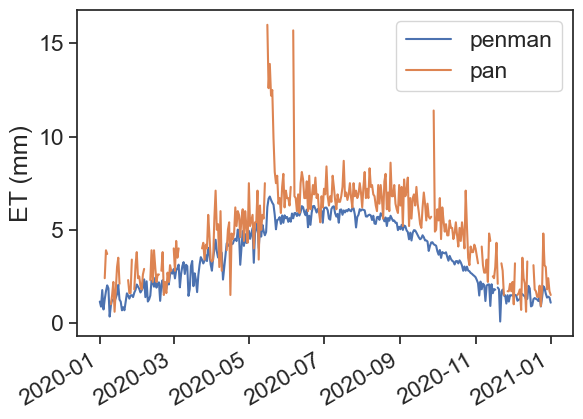
\includegraphics{introduction/introduction-exercises_files/figure-pdf/cell-9-output-1.png}

}

\end{figure}

\hypertarget{make-the-following-figure}{%
\section{make the following figure}\label{make-the-following-figure}}

Use the following function to plot bars for daily rainfall

\begin{Shaded}
\begin{Highlighting}[]
\NormalTok{ax.bar(x\_array, y\_array)}
\end{Highlighting}
\end{Shaded}

Can you write yourself some lines of code that calculate the cumulative
rainfall from the daily rainfall?

\begin{Shaded}
\begin{Highlighting}[]
\CommentTok{\#collapse{-}hide}

\CommentTok{\# creates figure (the canvas) and the axis (rectangle where the plot sits)}
\NormalTok{fig, ax }\OperatorTok{=}\NormalTok{ plt.subplots(}\DecValTok{1}\NormalTok{, figsize}\OperatorTok{=}\NormalTok{(}\DecValTok{10}\NormalTok{,}\DecValTok{7}\NormalTok{))}

\CommentTok{\# line and bar plots}
\NormalTok{ax.bar(df.index, df[}\StringTok{\textquotesingle{}rain24h\textquotesingle{}}\NormalTok{], color}\OperatorTok{=}\StringTok{"blue"}\NormalTok{, label}\OperatorTok{=}\StringTok{"daily rainfall"}\NormalTok{)}

\CommentTok{\# there are many ways of calculating the cumulative rain}

\CommentTok{\# method 1, use a for loop:}
\CommentTok{\# rain = df[\textquotesingle{}rain24h\textquotesingle{}].to\_numpy()}
\CommentTok{\# cumulative = rain * 0}
\CommentTok{\# for i in range(len(rain)):}
\CommentTok{\#     cumulative[i] = np.sum(rain[:i])}
\CommentTok{\# df[\textquotesingle{}cumulative1\textquotesingle{}] = cumulative}

\CommentTok{\# method 2, use list comprehension:}
\CommentTok{\# rain = df[\textquotesingle{}rain24h\textquotesingle{}].to\_numpy()}
\CommentTok{\# cumulative = [np.sum(rain[:i]) for i in range(len(rain))]}
\CommentTok{\# df[\textquotesingle{}cumulative2\textquotesingle{}] = cumulative}

\CommentTok{\# method 3, use existing functions:}
\NormalTok{df[}\StringTok{\textquotesingle{}cumulative3\textquotesingle{}}\NormalTok{] }\OperatorTok{=}\NormalTok{ np.cumsum(df[}\StringTok{\textquotesingle{}rain24h\textquotesingle{}}\NormalTok{])}

\NormalTok{ax.plot(df[}\StringTok{\textquotesingle{}cumulative3\textquotesingle{}}\NormalTok{], color}\OperatorTok{=}\StringTok{"red"}\NormalTok{, label}\OperatorTok{=}\StringTok{"cumulative rainfall"}\NormalTok{)}
\CommentTok{\# compare our cumulative rainfall with the downloaded data}
\CommentTok{\# ax.plot(df[\textquotesingle{}rain\_cumulative\textquotesingle{}], \textquotesingle{}x\textquotesingle{})}
\CommentTok{\# axes labels and figure title}
\NormalTok{ax.set\_xlabel(}\StringTok{\textquotesingle{}date\textquotesingle{}}\NormalTok{)}
\NormalTok{ax.set\_ylabel(}\StringTok{\textquotesingle{}rainfall (mm)\textquotesingle{}}\NormalTok{)}
\NormalTok{ax.set\_title(}\StringTok{\textquotesingle{}daily and cumulative rainfall\textquotesingle{}}\NormalTok{)}
\NormalTok{ax.set\_xlim([}\StringTok{\textquotesingle{}2020{-}11{-}01\textquotesingle{}}\NormalTok{,}\StringTok{\textquotesingle{}2021{-}02{-}28\textquotesingle{}}\NormalTok{])}
\CommentTok{\# some ticks adjustments}
\NormalTok{plt.gcf().autofmt\_xdate()  }\CommentTok{\# makes slated dates}
\CommentTok{\# legend}
\NormalTok{ax.legend(loc}\OperatorTok{=}\StringTok{\textquotesingle{}upper left\textquotesingle{}}\NormalTok{)}
\CommentTok{\# save png figure}
\NormalTok{plt.savefig(}\StringTok{"cumulative\_rainfall.png"}\NormalTok{)}
\end{Highlighting}
\end{Shaded}

\begin{figure}[H]

{\centering 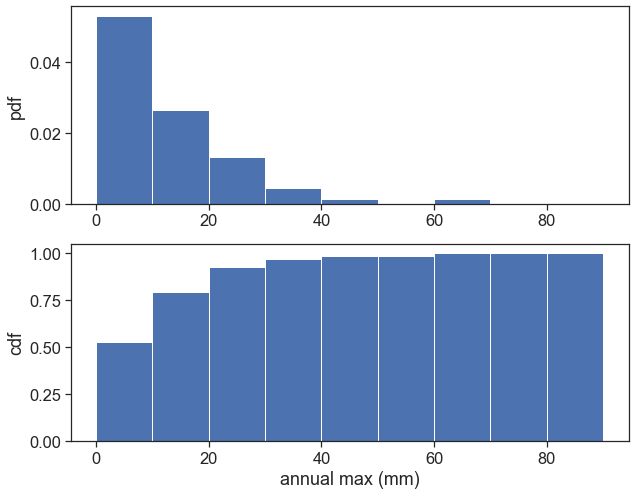
\includegraphics{introduction/introduction-exercises_files/figure-pdf/cell-10-output-1.png}

}

\end{figure}

\hypertarget{make-another-figure}{%
\section{make another figure}\label{make-another-figure}}

In order to choose just a part of the time series, you can use the
following:

\begin{Shaded}
\begin{Highlighting}[]
\NormalTok{start\_date }\OperatorTok{=} \StringTok{\textquotesingle{}2021{-}01{-}01\textquotesingle{}}
\NormalTok{end\_date }\OperatorTok{=} \StringTok{\textquotesingle{}2021{-}01{-}31\textquotesingle{}}
\NormalTok{january }\OperatorTok{=}\NormalTok{ df[start\_date:end\_date]}
\end{Highlighting}
\end{Shaded}

\begin{Shaded}
\begin{Highlighting}[]
\CommentTok{\#collapse{-}hide}

\CommentTok{\# creates figure (the canvas) and the axis (rectangle where the plot sits)}
\NormalTok{fig, ax }\OperatorTok{=}\NormalTok{ plt.subplots(}\DecValTok{1}\NormalTok{, figsize}\OperatorTok{=}\NormalTok{(}\DecValTok{10}\NormalTok{,}\DecValTok{7}\NormalTok{))}
\CommentTok{\# define date range}
\NormalTok{start\_date }\OperatorTok{=} \StringTok{\textquotesingle{}2021{-}01{-}01\textquotesingle{}}
\NormalTok{end\_date }\OperatorTok{=} \StringTok{\textquotesingle{}2021{-}01{-}31\textquotesingle{}}
\NormalTok{january }\OperatorTok{=}\NormalTok{ df[start\_date:end\_date][}\StringTok{\textquotesingle{}tmax\textquotesingle{}}\NormalTok{]}
\CommentTok{\# plots}
\NormalTok{ax.plot(january, color}\OperatorTok{=}\StringTok{"red"}\NormalTok{, label}\OperatorTok{=}\StringTok{"daily max"}\NormalTok{)}
\NormalTok{ax.plot(january}\OperatorTok{*}\DecValTok{0} \OperatorTok{+}\NormalTok{ january.mean(), color}\OperatorTok{=}\StringTok{"purple"}\NormalTok{, linestyle}\OperatorTok{=}\StringTok{"{-}{-}"}\NormalTok{, label}\OperatorTok{=}\StringTok{"average daily max"}\NormalTok{)}
\CommentTok{\# axes labels and figure title}
\NormalTok{ax.set\_xlabel(}\StringTok{\textquotesingle{}date\textquotesingle{}}\NormalTok{)}
\NormalTok{ax.set\_ylabel(}\StringTok{\textquotesingle{}temperature (°C)\textquotesingle{}}\NormalTok{)}
\NormalTok{ax.set\_title(}\StringTok{\textquotesingle{}average daily maximum temperature for January 2021\textquotesingle{}}\NormalTok{)}
\CommentTok{\# some ticks adjustments}
\NormalTok{plt.gcf().autofmt\_xdate()  }\CommentTok{\# makes slated dates}
\CommentTok{\# legend}
\NormalTok{ax.legend(loc}\OperatorTok{=}\StringTok{\textquotesingle{}lower left\textquotesingle{}}\NormalTok{)}
\CommentTok{\# save png figure}
\NormalTok{plt.savefig(}\StringTok{"average\_max\_temp.png"}\NormalTok{)}
\end{Highlighting}
\end{Shaded}

\begin{figure}[H]

{\centering 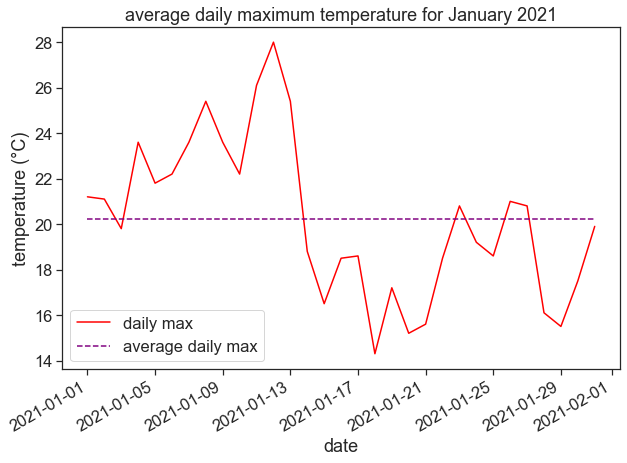
\includegraphics{introduction/introduction-exercises_files/figure-pdf/cell-11-output-1.png}

}

\end{figure}

\hypertarget{one-last-figure-for-today}{%
\section{one last figure for today}\label{one-last-figure-for-today}}

Use the following code to create histograms with user-defined bins:

\begin{Shaded}
\begin{Highlighting}[]
\NormalTok{b }\OperatorTok{=}\NormalTok{ np.arange(}\DecValTok{0}\NormalTok{, }\DecValTok{56}\NormalTok{, }\DecValTok{5}\NormalTok{)  }\CommentTok{\# bins from 0 to 55, width = 5}
\NormalTok{ax.hist(df[}\StringTok{\textquotesingle{}wind\textquotesingle{}}\NormalTok{], bins}\OperatorTok{=}\NormalTok{b, density}\OperatorTok{=}\VariableTok{True}\NormalTok{)}
\end{Highlighting}
\end{Shaded}

Play with the bins, see what happens. What does \texttt{density=True}
do?

\begin{Shaded}
\begin{Highlighting}[]
\CommentTok{\# creates figure (the canvas) and the axis (rectangle where the plot sits)}
\NormalTok{fig, ax }\OperatorTok{=}\NormalTok{ plt.subplots(}\DecValTok{1}\NormalTok{, figsize}\OperatorTok{=}\NormalTok{(}\DecValTok{10}\NormalTok{,}\DecValTok{7}\NormalTok{))}
\CommentTok{\# histogram}
\NormalTok{b }\OperatorTok{=}\NormalTok{ np.arange(}\DecValTok{0}\NormalTok{, }\DecValTok{56}\NormalTok{, }\DecValTok{5}\NormalTok{)  }\CommentTok{\# bins from 0 to 55, width = 5}
\NormalTok{ax.hist(df[}\StringTok{\textquotesingle{}wind\textquotesingle{}}\NormalTok{], bins}\OperatorTok{=}\NormalTok{b, density}\OperatorTok{=}\VariableTok{True}\NormalTok{)}
\CommentTok{\# axes labels and figure title}
\NormalTok{ax.set\_xlabel(}\StringTok{\textquotesingle{}max wind speed (km/h)\textquotesingle{}}\NormalTok{)}
\NormalTok{ax.set\_ylabel(}\StringTok{\textquotesingle{}frequency\textquotesingle{}}\NormalTok{)}
\NormalTok{ax.set\_title(}\StringTok{\textquotesingle{}frequency of maximum wind speed\textquotesingle{}}\NormalTok{)}
\CommentTok{\# save png figure}
\NormalTok{plt.savefig(}\StringTok{"wind{-}histogram.png"}\NormalTok{)}
\end{Highlighting}
\end{Shaded}

\begin{figure}[H]

{\centering 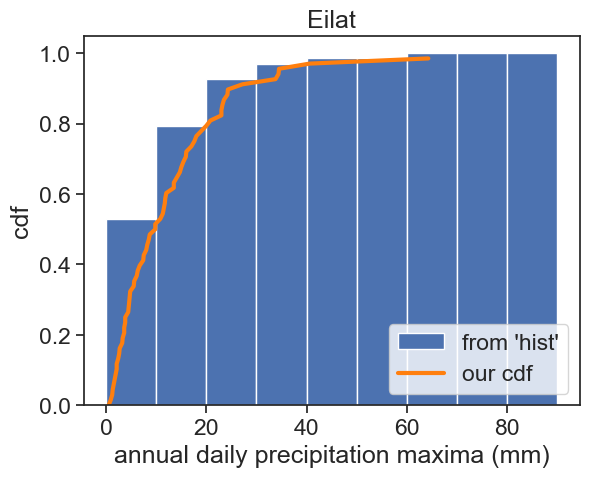
\includegraphics{introduction/introduction-exercises_files/figure-pdf/cell-12-output-1.png}

}

\end{figure}

\hypertarget{homework}{%
\chapter{homework}\label{homework}}

Go back to the weather station website, download one year of data from
01.01.2020 to 31.12.2020 (24h data). If you can't download the data,
just click \href{https://yairmau.com/archive/hydrology/1year.csv}{here}.
Make the following graph: - daily tmax and tmin - smoothed data for tmax
and tmin

In order to smooth the data with a 30 day window, use the following
function:\\
\texttt{df{[}\textquotesingle{}tmin\textquotesingle{}{]}.rolling(30,\ center=True).mean()}\strut \\
This means that you will take the mean of 30 days, and put the result in
the center of this 30-day window.

Play with this function, see what you can do with it. What happens when
you change the size of the window? Why is the smoothed data shorter than
the original data? See the
\href{https://pandas.pydata.org/pandas-docs/stable/reference/api/pandas.DataFrame.rolling.html}{documentation}
for \texttt{rolling} to find more options.

\begin{Shaded}
\begin{Highlighting}[]
\CommentTok{\#collapse{-}hide}

\NormalTok{fig, ax }\OperatorTok{=}\NormalTok{ plt.subplots(figsize}\OperatorTok{=}\NormalTok{(}\DecValTok{10}\NormalTok{,}\DecValTok{7}\NormalTok{))}
\NormalTok{df2 }\OperatorTok{=}\NormalTok{ pd.read\_csv(}\StringTok{"1year.csv"}\NormalTok{, header}\OperatorTok{=}\NormalTok{[}\DecValTok{4}\NormalTok{])}
\NormalTok{df2[}\StringTok{\textquotesingle{}date\textquotesingle{}}\NormalTok{] }\OperatorTok{=}\NormalTok{ pd.to\_datetime(df2[}\StringTok{\textquotesingle{}date\textquotesingle{}}\NormalTok{], dayfirst}\OperatorTok{=}\VariableTok{True}\NormalTok{)}
\NormalTok{df2 }\OperatorTok{=}\NormalTok{ df2.set\_index(}\StringTok{\textquotesingle{}date\textquotesingle{}}\NormalTok{)}
\NormalTok{plt.plot(df2[}\StringTok{\textquotesingle{}tmax\textquotesingle{}}\NormalTok{], label}\OperatorTok{=}\StringTok{\textquotesingle{}tmax\textquotesingle{}}\NormalTok{, color}\OperatorTok{=}\StringTok{"tab:red"}\NormalTok{)}
\NormalTok{plt.plot(df2[}\StringTok{\textquotesingle{}tmin\textquotesingle{}}\NormalTok{], label}\OperatorTok{=}\StringTok{\textquotesingle{}tmin\textquotesingle{}}\NormalTok{, color}\OperatorTok{=}\StringTok{"tab:blue"}\NormalTok{)}
\NormalTok{tmin\_smooth }\OperatorTok{=}\NormalTok{ df2[}\StringTok{\textquotesingle{}tmin\textquotesingle{}}\NormalTok{].rolling(}\DecValTok{30}\NormalTok{, center}\OperatorTok{=}\VariableTok{True}\NormalTok{).mean()}
\NormalTok{tmax\_smooth }\OperatorTok{=}\NormalTok{ df2[}\StringTok{\textquotesingle{}tmax\textquotesingle{}}\NormalTok{].rolling(}\DecValTok{30}\NormalTok{, center}\OperatorTok{=}\VariableTok{True}\NormalTok{).mean()}
\NormalTok{plt.plot(tmax\_smooth, label}\OperatorTok{=}\StringTok{\textquotesingle{}tmax smoothed\textquotesingle{}}\NormalTok{, color}\OperatorTok{=}\StringTok{"tab:pink"}\NormalTok{, linestyle}\OperatorTok{=}\StringTok{"{-}{-}"}\NormalTok{, linewidth}\OperatorTok{=}\DecValTok{3}\NormalTok{)}
\NormalTok{plt.plot(tmin\_smooth, label}\OperatorTok{=}\StringTok{\textquotesingle{}tmin smoothed\textquotesingle{}}\NormalTok{, color}\OperatorTok{=}\StringTok{"tab:cyan"}\NormalTok{, linestyle}\OperatorTok{=}\StringTok{"{-}{-}"}\NormalTok{, linewidth}\OperatorTok{=}\DecValTok{3}\NormalTok{)}
\NormalTok{plt.legend()}
\NormalTok{plt.savefig(}\StringTok{"t\_smoothed.png"}\NormalTok{)}
\end{Highlighting}
\end{Shaded}

\begin{figure}[H]

{\centering 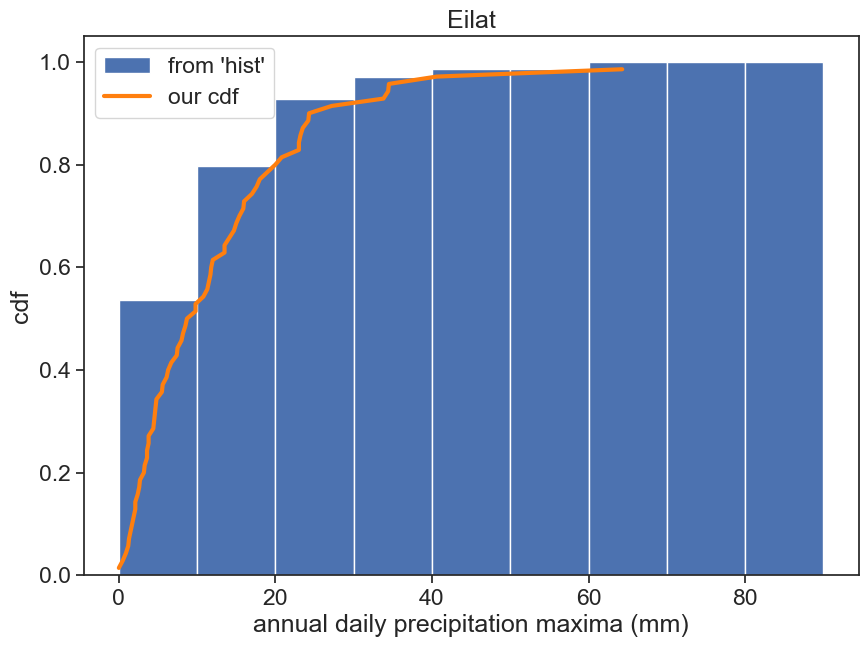
\includegraphics{introduction/introduction-exercises_files/figure-pdf/cell-13-output-1.png}

}

\end{figure}

\part{Precipitation}

\hypertarget{interannual-variability-of-precipitation}{%
\chapter{Interannual variability of
precipitation}\label{interannual-variability-of-precipitation}}

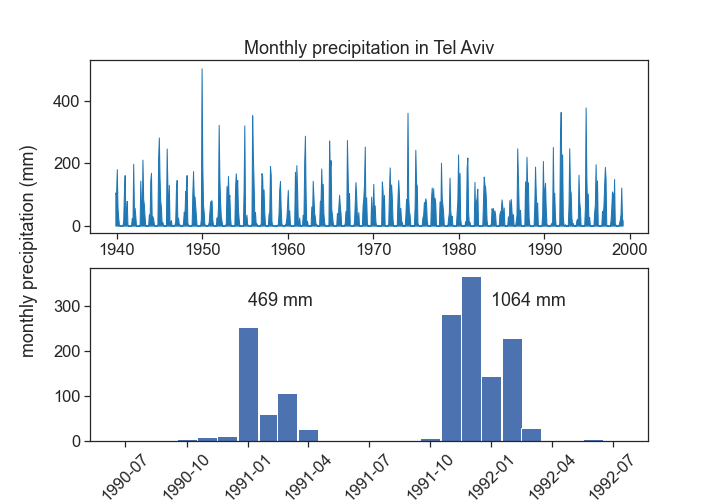
\includegraphics{archive/figures/monthly_tel_aviv_1940-1999.png}

A time period of 12 months for which precipitation totals are measured.
The hydrological year is designated by the calendar year in which it
\textbf{ends}.\\
Let's define the hydrological year for Tel Aviv from 1 October to 30
September.

האם אקלים הגשם שלנו משתנה \textgreater{} youtube:
https://youtu.be/v0uNpj03Rk4

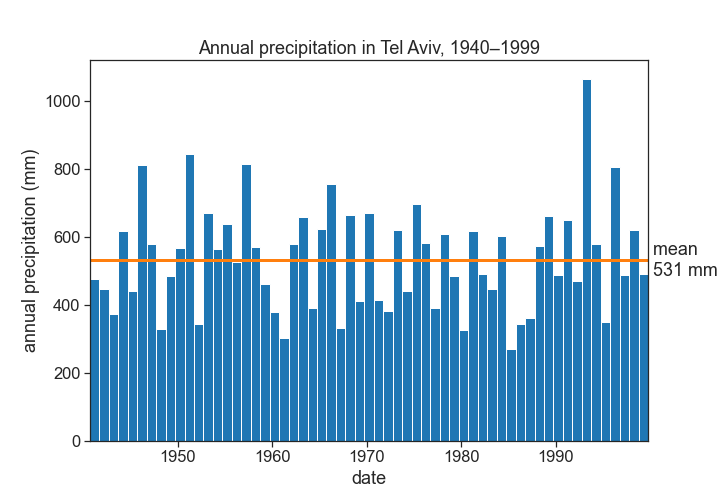
\includegraphics{archive/figures/annual_tel_aviv_with_mean.png}

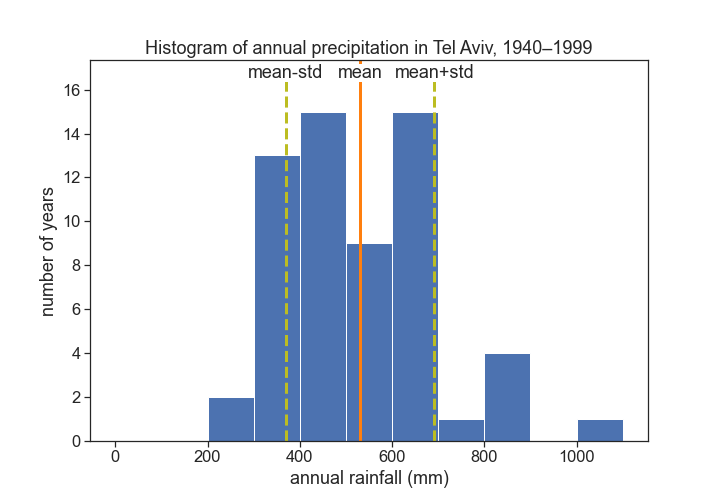
\includegraphics{archive/figures/histogram_tel_aviv_with_mean_and_std.png}

\hypertarget{coefficient-of-variation}{%
\section{coefficient of variation}\label{coefficient-of-variation}}

\(\langle{P}\rangle=\) average precipitation\\
\(\sigma=\) standard deviation

\[CV = \frac{\sigma}{\langle{P}\rangle}\]

Assuming that the inter-annual distribution is a gaussian: 67\% of the
time, rainfall will vary +/- 30\% from its long term average in Tel
Aviv.

Precipitation averages are
\href{https://www.ncdc.noaa.gov/news/defining-climate-normals-new-ways}{usually
calculated for time intervals of 30 years}.

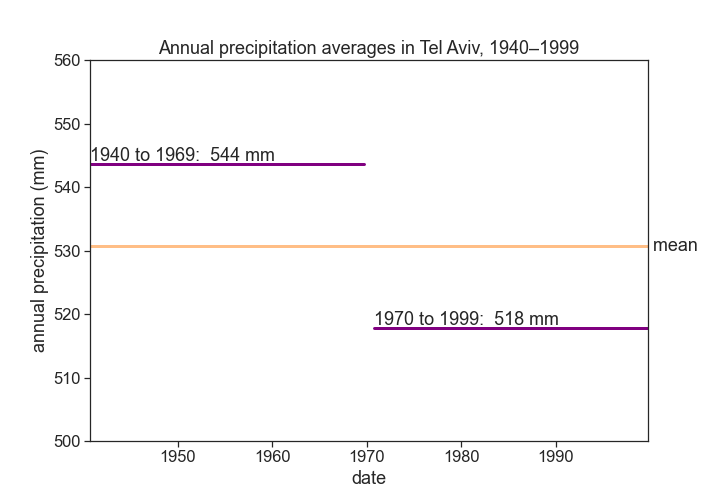
\includegraphics{archive/figures/mean_tel_aviv_2_windows.png}

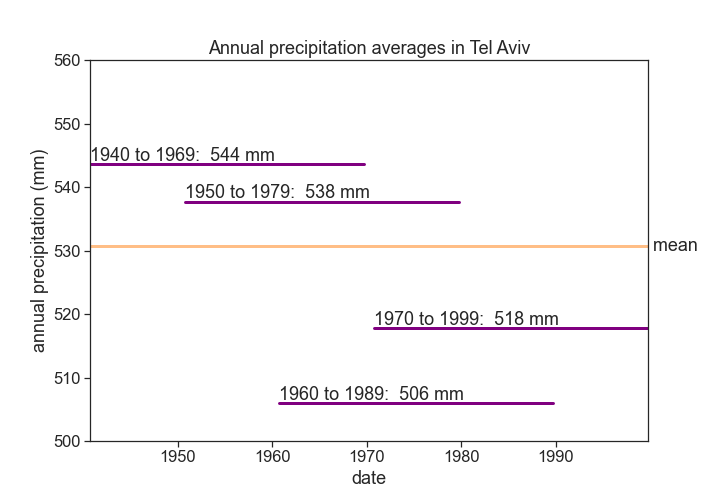
\includegraphics{archive/figures/mean_tel_aviv_4_windows.png}

\begin{Shaded}
\begin{Highlighting}[]
\ImportTok{import}\NormalTok{ altair }\ImportTok{as}\NormalTok{ alt}
\ImportTok{import}\NormalTok{ pandas }\ImportTok{as}\NormalTok{ pd}

\NormalTok{df }\OperatorTok{=}\NormalTok{ pd.read\_csv(}\StringTok{"TEL\_AVIV\_READING\_monthly.csv"}\NormalTok{, sep}\OperatorTok{=}\StringTok{","}\NormalTok{)}
\CommentTok{\# make \textquotesingle{}DATE\textquotesingle{} the dataframe index}
\NormalTok{df[}\StringTok{\textquotesingle{}DATE\textquotesingle{}}\NormalTok{] }\OperatorTok{=}\NormalTok{ pd.to\_datetime(df[}\StringTok{\textquotesingle{}DATE\textquotesingle{}}\NormalTok{])}
\NormalTok{df }\OperatorTok{=}\NormalTok{ df.set\_index(}\StringTok{\textquotesingle{}DATE\textquotesingle{}}\NormalTok{)}

\NormalTok{df\_year\_all }\OperatorTok{=}\NormalTok{ df[}\StringTok{\textquotesingle{}PRCP\textquotesingle{}}\NormalTok{].resample(}\StringTok{\textquotesingle{}A{-}SEP\textquotesingle{}}\NormalTok{).}\BuiltInTok{sum}\NormalTok{().to\_frame()  }\CommentTok{\# annual frequency, anchored end of September}
\NormalTok{df\_year\_all.columns }\OperatorTok{=}\NormalTok{ [}\StringTok{\textquotesingle{}rain (mm)\textquotesingle{}}\NormalTok{] }\CommentTok{\# rename \textquotesingle{}PRCP\textquotesingle{} column to \textquotesingle{}rain (mm)\textquotesingle{}}
\NormalTok{df\_year }\OperatorTok{=}\NormalTok{ df\_year\_all.iloc[:}\OperatorTok{{-}}\DecValTok{1}\NormalTok{]  }\CommentTok{\# exclude last row}

\CommentTok{\# Altair only recognizes column data; it ignores index values.}
\CommentTok{\# You can plot the index data by first resetting the index}
\CommentTok{\# I know that I\textquotesingle{}ve just made \textquotesingle{}DATE\textquotesingle{} the index, but I want to have this here nonetheless so I can refer to this in the future}
\NormalTok{source }\OperatorTok{=}\NormalTok{ df\_year.reset\_index()}
\NormalTok{brush }\OperatorTok{=}\NormalTok{ alt.selection(}\BuiltInTok{type}\OperatorTok{=}\StringTok{\textquotesingle{}interval\textquotesingle{}}\NormalTok{, encodings}\OperatorTok{=}\NormalTok{[}\StringTok{\textquotesingle{}x\textquotesingle{}}\NormalTok{])}

\CommentTok{\# T: temporal, a time or date value}
\CommentTok{\# Q: quantitative, a continuous real{-}valued quantity}
\CommentTok{\# https://altair{-}viz.github.io/user\_guide/encoding.html\#encoding{-}data{-}types}
\NormalTok{bars }\OperatorTok{=}\NormalTok{ alt.Chart().mark\_bar().encode(}
\NormalTok{    x}\OperatorTok{=}\NormalTok{alt.X(}\StringTok{\textquotesingle{}DATE:T\textquotesingle{}}\NormalTok{, axis}\OperatorTok{=}\NormalTok{alt.Axis(title}\OperatorTok{=}\StringTok{\textquotesingle{}date\textquotesingle{}}\NormalTok{)),}
\NormalTok{    y}\OperatorTok{=}\NormalTok{alt.Y(}\StringTok{\textquotesingle{}rain (mm):Q\textquotesingle{}}\NormalTok{,  axis}\OperatorTok{=}\NormalTok{alt.Axis(title}\OperatorTok{=}\StringTok{\textquotesingle{}annual precipitation (mm) and average\textquotesingle{}}\NormalTok{)),}
\NormalTok{    opacity}\OperatorTok{=}\NormalTok{alt.condition(brush, alt.OpacityValue(}\DecValTok{1}\NormalTok{), alt.OpacityValue(}\FloatTok{0.2}\NormalTok{)),}
\NormalTok{).add\_selection(}
\NormalTok{    brush}
\NormalTok{).properties(}
\NormalTok{    title}\OperatorTok{=}\StringTok{\textquotesingle{}Select year range and drag for rolling average of annual precipitation in Tel Aviv\textquotesingle{}}
\NormalTok{).properties(}
\NormalTok{    width}\OperatorTok{=}\DecValTok{600}\NormalTok{,}
\NormalTok{    height}\OperatorTok{=}\DecValTok{400}
\NormalTok{)}

\NormalTok{line }\OperatorTok{=}\NormalTok{ alt.Chart().mark\_rule(color}\OperatorTok{=}\StringTok{\textquotesingle{}orange\textquotesingle{}}\NormalTok{).encode(}
\NormalTok{    y}\OperatorTok{=}\StringTok{\textquotesingle{}mean(rain (mm)):Q\textquotesingle{}}\NormalTok{,}
\NormalTok{    size}\OperatorTok{=}\NormalTok{alt.SizeValue(}\DecValTok{3}\NormalTok{)}
\NormalTok{).transform\_filter(}
\NormalTok{    brush}
\NormalTok{)}

\NormalTok{alt.layer(bars, line, data}\OperatorTok{=}\NormalTok{source)}
\end{Highlighting}
\end{Shaded}

\begin{verbatim}
alt.LayerChart(...)
\end{verbatim}

\hypertarget{exercises-1}{%
\chapter{Exercises}\label{exercises-1}}

Import relevant packages

\begin{Shaded}
\begin{Highlighting}[]
\ImportTok{import}\NormalTok{ matplotlib.pyplot }\ImportTok{as}\NormalTok{ plt}
\ImportTok{import}\NormalTok{ numpy }\ImportTok{as}\NormalTok{ np}
\ImportTok{import}\NormalTok{ pandas }\ImportTok{as}\NormalTok{ pd}
\ImportTok{from}\NormalTok{ calendar }\ImportTok{import}\NormalTok{ month\_abbr}
\ImportTok{import}\NormalTok{ seaborn }\ImportTok{as}\NormalTok{ sns}
\NormalTok{sns.}\BuiltInTok{set}\NormalTok{(style}\OperatorTok{=}\StringTok{"ticks"}\NormalTok{, font\_scale}\OperatorTok{=}\FloatTok{1.5}\NormalTok{)}
\ImportTok{import}\NormalTok{ urllib.request}
\ImportTok{from}\NormalTok{ pandas.plotting }\ImportTok{import}\NormalTok{ register\_matplotlib\_converters}
\NormalTok{register\_matplotlib\_converters()}
\end{Highlighting}
\end{Shaded}

Plot monthly rainfall for your station.

Load the data into a datafram, and before you continue with the
analysis, plot the rainfall data, to see how it looks like.

\begin{Shaded}
\begin{Highlighting}[]
\NormalTok{df }\OperatorTok{=}\NormalTok{ pd.read\_csv(}\StringTok{\textquotesingle{}BEN\_GURION\_monthly.csv\textquotesingle{}}\NormalTok{, sep}\OperatorTok{=}\StringTok{","}\NormalTok{)}
\NormalTok{df[}\StringTok{\textquotesingle{}DATE\textquotesingle{}}\NormalTok{] }\OperatorTok{=}\NormalTok{ pd.to\_datetime(df[}\StringTok{\textquotesingle{}DATE\textquotesingle{}}\NormalTok{])}
\NormalTok{df }\OperatorTok{=}\NormalTok{ df.set\_index(}\StringTok{\textquotesingle{}DATE\textquotesingle{}}\NormalTok{)}

\NormalTok{fig, (ax1, ax2) }\OperatorTok{=}\NormalTok{ plt.subplots(}\DecValTok{2}\NormalTok{, }\DecValTok{1}\NormalTok{, figsize}\OperatorTok{=}\NormalTok{(}\DecValTok{10}\NormalTok{,}\DecValTok{7}\NormalTok{))}
\NormalTok{ax1.plot(df[}\StringTok{\textquotesingle{}PRCP\textquotesingle{}}\NormalTok{])}
\NormalTok{ax2.plot(df[}\StringTok{\textquotesingle{}PRCP\textquotesingle{}}\NormalTok{][}\StringTok{\textquotesingle{}2010{-}07{-}01\textquotesingle{}}\NormalTok{:}\StringTok{\textquotesingle{}2015{-}07{-}01\textquotesingle{}}\NormalTok{])}
\end{Highlighting}
\end{Shaded}

\begin{figure}[H]

{\centering 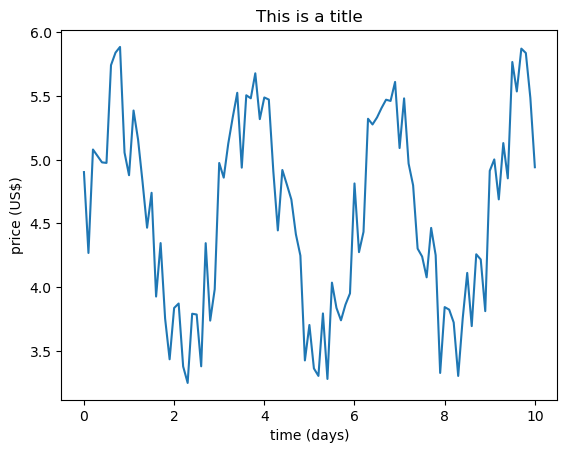
\includegraphics{precipitation/interannual-exercises_files/figure-pdf/cell-3-output-1.png}

}

\end{figure}

How to aggregate rainfall accoding to the hydrological year? We use the
function \texttt{resample}.

read more about resampling options:\\
\url{https://pandas.pydata.org/pandas-docs/version/0.12.0/timeseries.html\#offset-aliases}

also, annual resampling can be anchored to the end of specific months:
\url{https://pandas.pydata.org/pandas-docs/version/0.12.0/timeseries.html\#anchored-offsets}

\begin{Shaded}
\begin{Highlighting}[]
\CommentTok{\# annual frequency, anchored 31 December}
\NormalTok{df\_year\_all }\OperatorTok{=}\NormalTok{ df[}\StringTok{\textquotesingle{}PRCP\textquotesingle{}}\NormalTok{].resample(}\StringTok{\textquotesingle{}A\textquotesingle{}}\NormalTok{).}\BuiltInTok{sum}\NormalTok{().to\_frame()}
\CommentTok{\# annual frequency, anchored 01 January}
\NormalTok{df\_year\_all }\OperatorTok{=}\NormalTok{ df[}\StringTok{\textquotesingle{}PRCP\textquotesingle{}}\NormalTok{].resample(}\StringTok{\textquotesingle{}AS\textquotesingle{}}\NormalTok{).}\BuiltInTok{sum}\NormalTok{().to\_frame()}
\CommentTok{\# annual frequency, anchored end of September}
\NormalTok{df\_year\_all }\OperatorTok{=}\NormalTok{ df[}\StringTok{\textquotesingle{}PRCP\textquotesingle{}}\NormalTok{].resample(}\StringTok{\textquotesingle{}A{-}SEP\textquotesingle{}}\NormalTok{).}\BuiltInTok{sum}\NormalTok{().to\_frame()}
\CommentTok{\# rename \textquotesingle{}PRCP\textquotesingle{} column to \textquotesingle{}rain (mm)\textquotesingle{}}
\NormalTok{df\_year\_all.columns }\OperatorTok{=}\NormalTok{ [}\StringTok{\textquotesingle{}rain (mm)\textquotesingle{}}\NormalTok{]}
\NormalTok{df\_year\_all}
\end{Highlighting}
\end{Shaded}

\begin{longtable}[]{@{}ll@{}}
\toprule()
& rain (mm) \\
DATE & \\
\midrule()
\endhead
1922-09-30 & 136.6 \\
1923-09-30 & 144.5 \\
1924-09-30 & 130.4 \\
1925-09-30 & 165.3 \\
1926-09-30 & 188.7 \\
... & ... \\
2012-09-30 & 145.7 \\
2013-09-30 & 175.3 \\
2014-09-30 & 259.2 \\
2015-09-30 & 249.3 \\
2016-09-30 & 257.6 \\
\bottomrule()
\end{longtable}

You might need to exclude the first or the last line, since their data
might have less that 12 months. For example:

\begin{Shaded}
\begin{Highlighting}[]
\CommentTok{\# exclude 1st row}
\NormalTok{df\_year }\OperatorTok{=}\NormalTok{ df\_year\_all.iloc[}\DecValTok{1}\NormalTok{:]}
\CommentTok{\# exclude last row}
\NormalTok{df\_year }\OperatorTok{=}\NormalTok{ df\_year\_all.iloc[:}\OperatorTok{{-}}\DecValTok{1}\NormalTok{]}
\CommentTok{\# exclude both 1st and last rows}
\NormalTok{df\_year }\OperatorTok{=}\NormalTok{ df\_year\_all.iloc[}\DecValTok{1}\NormalTok{:}\OperatorTok{{-}}\DecValTok{1}\NormalTok{]}
\NormalTok{df\_year}
\end{Highlighting}
\end{Shaded}

\begin{longtable}[]{@{}ll@{}}
\toprule()
& rain (mm) \\
DATE & \\
\midrule()
\endhead
1923-09-30 & 144.5 \\
1924-09-30 & 130.4 \\
1925-09-30 & 165.3 \\
1926-09-30 & 188.7 \\
1927-09-30 & 130.2 \\
... & ... \\
2011-09-30 & 151.6 \\
2012-09-30 & 145.7 \\
2013-09-30 & 175.3 \\
2014-09-30 & 259.2 \\
2015-09-30 & 249.3 \\
\bottomrule()
\end{longtable}

Calculate the average annual rainfall. Plot annual rainfall for the
whole range, together with the average. You should get something like
this:

\begin{Shaded}
\begin{Highlighting}[]
\NormalTok{fig, ax }\OperatorTok{=}\NormalTok{ plt.subplots(figsize}\OperatorTok{=}\NormalTok{(}\DecValTok{10}\NormalTok{,}\DecValTok{7}\NormalTok{))}

\CommentTok{\# plot YEARLY precipitation}
\NormalTok{ax.bar(df\_year.index, df\_year[}\StringTok{\textquotesingle{}rain (mm)\textquotesingle{}}\NormalTok{],}
\NormalTok{       width}\OperatorTok{=}\DecValTok{365}\NormalTok{, align}\OperatorTok{=}\StringTok{\textquotesingle{}edge\textquotesingle{}}\NormalTok{, color}\OperatorTok{=}\StringTok{"tab:blue"}\NormalTok{)}

\CommentTok{\# plot mean}
\NormalTok{rain\_mean }\OperatorTok{=}\NormalTok{ df\_year[}\StringTok{\textquotesingle{}rain (mm)\textquotesingle{}}\NormalTok{].mean()}
\NormalTok{ax.plot(ax.get\_xlim(), [rain\_mean]}\OperatorTok{*}\DecValTok{2}\NormalTok{, linewidth}\OperatorTok{=}\DecValTok{3}\NormalTok{, color}\OperatorTok{=}\StringTok{"tab:orange"}\NormalTok{)}
\NormalTok{ax.}\BuiltInTok{set}\NormalTok{(xlabel}\OperatorTok{=}\StringTok{"date"}\NormalTok{,}
\NormalTok{       ylabel}\OperatorTok{=}\StringTok{"yearly rainfall (mm)"}\NormalTok{,}
\NormalTok{       title}\OperatorTok{=}\SpecialStringTok{f"Beer Sheva, mean = }\SpecialCharTok{\{}\NormalTok{rain\_mean}\SpecialCharTok{:.0f\}}\SpecialStringTok{ mm"}\NormalTok{)}\OperatorTok{;}
\CommentTok{\# save figure}
\CommentTok{\# plt.savefig("hydrology\_figures/beersheva\_yearly\_rainfall\_1923\_2016.png")}
\end{Highlighting}
\end{Shaded}

\begin{figure}[H]

{\centering 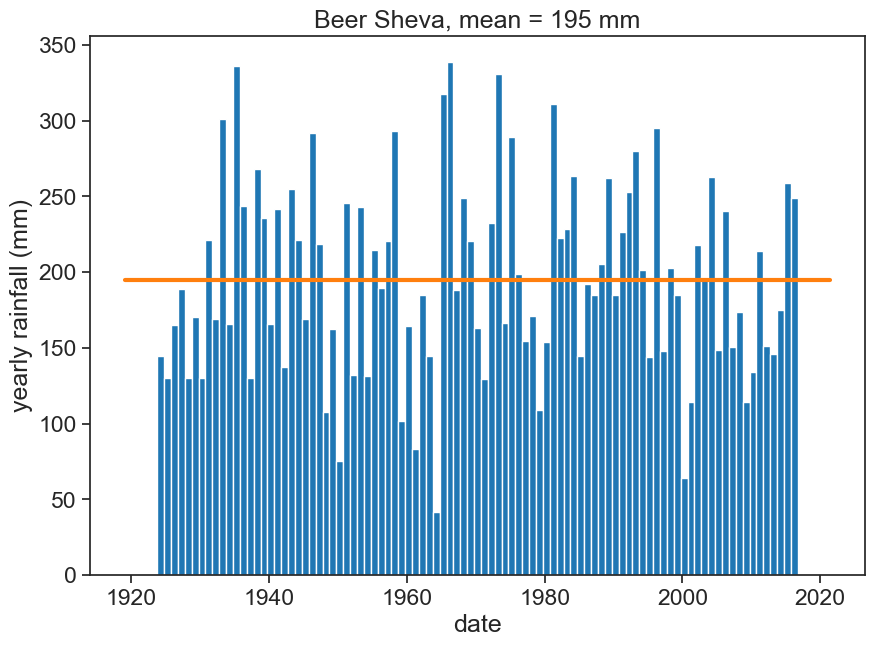
\includegraphics{precipitation/interannual-exercises_files/figure-pdf/cell-6-output-1.png}

}

\end{figure}

Plot a histogram of annual rainfall, with the mean and standard
deviation. Calculate the coefficient of variation. Try to plot something
like this:

\begin{Shaded}
\begin{Highlighting}[]
\NormalTok{fig, ax }\OperatorTok{=}\NormalTok{ plt.subplots(figsize}\OperatorTok{=}\NormalTok{(}\DecValTok{10}\NormalTok{,}\DecValTok{7}\NormalTok{))}

\CommentTok{\# calculate mean and standard deviation}
\NormalTok{rain\_mean }\OperatorTok{=}\NormalTok{ df\_year[}\StringTok{\textquotesingle{}rain (mm)\textquotesingle{}}\NormalTok{].mean()}
\NormalTok{rain\_std }\OperatorTok{=}\NormalTok{ df\_year[}\StringTok{\textquotesingle{}rain (mm)\textquotesingle{}}\NormalTok{].std()}

\CommentTok{\# plot histogram}
\NormalTok{b }\OperatorTok{=}\NormalTok{ np.arange(}\DecValTok{0}\NormalTok{, }\DecValTok{401}\NormalTok{, }\DecValTok{50}\NormalTok{)  }\CommentTok{\# bins from 0 to 400, width = 50}
\NormalTok{ax.hist(df\_year[}\StringTok{\textquotesingle{}rain (mm)\textquotesingle{}}\NormalTok{], bins}\OperatorTok{=}\NormalTok{b)}

\CommentTok{\# plot vertical lines with mean, std, etc}
\NormalTok{ylim }\OperatorTok{=}\NormalTok{ np.array(ax.get\_ylim())}
\NormalTok{ylim[}\DecValTok{1}\NormalTok{] }\OperatorTok{=}\NormalTok{ ylim[}\DecValTok{1}\NormalTok{]}\OperatorTok{*}\FloatTok{1.1}
\NormalTok{ax.plot([rain\_mean]}\OperatorTok{*}\DecValTok{2}\NormalTok{, ylim, linewidth}\OperatorTok{=}\DecValTok{3}\NormalTok{, color}\OperatorTok{=}\StringTok{"tab:orange"}\NormalTok{)}
\NormalTok{ax.plot([rain\_mean}\OperatorTok{+}\NormalTok{rain\_std]}\OperatorTok{*}\DecValTok{2}\NormalTok{, ylim, linewidth}\OperatorTok{=}\DecValTok{3}\NormalTok{, linestyle}\OperatorTok{=}\StringTok{"{-}{-}"}\NormalTok{, color}\OperatorTok{=}\StringTok{"tab:olive"}\NormalTok{)}
\NormalTok{ax.plot([rain\_mean}\OperatorTok{{-}}\NormalTok{rain\_std]}\OperatorTok{*}\DecValTok{2}\NormalTok{, ylim, linewidth}\OperatorTok{=}\DecValTok{3}\NormalTok{, linestyle}\OperatorTok{=}\StringTok{"{-}{-}"}\NormalTok{, color}\OperatorTok{=}\StringTok{"tab:olive"}\NormalTok{)}
\NormalTok{ax.}\BuiltInTok{set}\NormalTok{(ylim}\OperatorTok{=}\NormalTok{ylim,}
\NormalTok{       xlabel}\OperatorTok{=}\StringTok{"annual rainfall (mm)"}\NormalTok{,}
\NormalTok{       ylabel}\OperatorTok{=}\StringTok{"number of years"}\NormalTok{,}
\NormalTok{       title}\OperatorTok{=}\SpecialStringTok{f"Beer Sheva, 1922–2016. Mean=}\SpecialCharTok{\{}\NormalTok{rain\_mean}\SpecialCharTok{:.0f\}}\SpecialStringTok{ mm, STD=}\SpecialCharTok{\{}\NormalTok{rain\_std}\SpecialCharTok{:.0f\}}\SpecialStringTok{ mm"}\NormalTok{)}
\NormalTok{ax.text(}\DecValTok{300}\NormalTok{, }\DecValTok{25}\NormalTok{, }\SpecialStringTok{f"CV = }\SpecialCharTok{\{}\NormalTok{rain\_std}\OperatorTok{/}\NormalTok{rain\_mean}\SpecialCharTok{:.2f\}}\SpecialStringTok{"}\NormalTok{)}
\NormalTok{plt.savefig(}\StringTok{"histogram\_beersheva.png"}\NormalTok{)}
\end{Highlighting}
\end{Shaded}

\begin{figure}[H]

{\centering 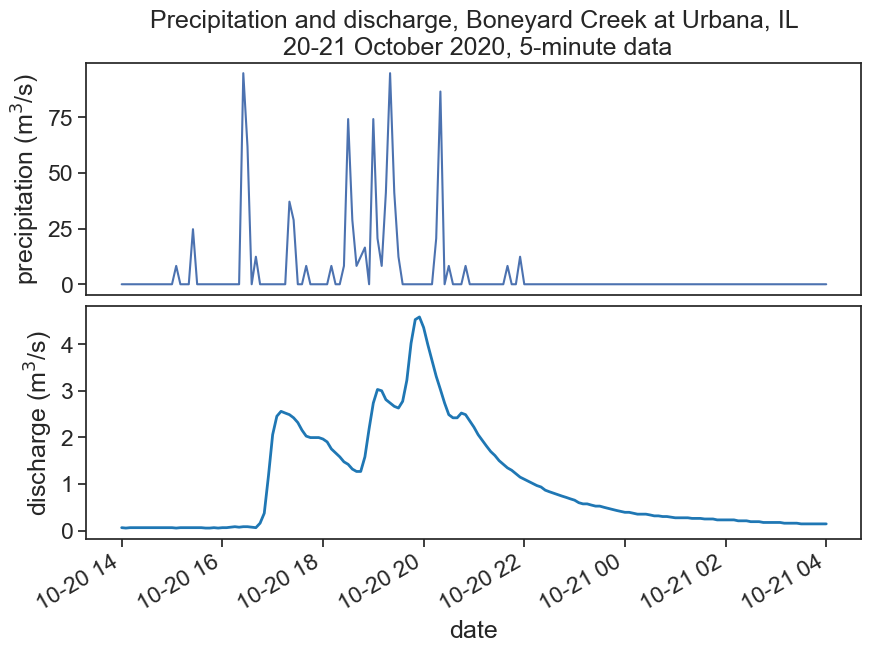
\includegraphics{precipitation/interannual-exercises_files/figure-pdf/cell-7-output-1.png}

}

\end{figure}

Calculate the mean annual rainfall for various 30-year intervals

\begin{Shaded}
\begin{Highlighting}[]
\CommentTok{\#\#\#\#\#\#\# the hard way \#\#\#\#\#\#\#}
\CommentTok{\# fig, ax = plt.subplots(figsize=(10,7))}

\CommentTok{\# mean\_30\_59 = df\_year.loc[\textquotesingle{}1930{-}09{-}30\textquotesingle{}:\textquotesingle{}1959{-}09{-}01\textquotesingle{},\textquotesingle{}rain (mm)\textquotesingle{}].mean()}
\CommentTok{\# mean\_40\_69 = df\_year.loc[\textquotesingle{}1940{-}09{-}30\textquotesingle{}:\textquotesingle{}1969{-}09{-}01\textquotesingle{},\textquotesingle{}rain (mm)\textquotesingle{}].mean()}
\CommentTok{\# mean\_50\_79 = df\_year.loc[\textquotesingle{}1950{-}09{-}30\textquotesingle{}:\textquotesingle{}1979{-}09{-}01\textquotesingle{},\textquotesingle{}rain (mm)\textquotesingle{}].mean()}
\CommentTok{\# mean\_60\_89 = df\_year.loc[\textquotesingle{}1960{-}09{-}30\textquotesingle{}:\textquotesingle{}1989{-}09{-}01\textquotesingle{},\textquotesingle{}rain (mm)\textquotesingle{}].mean()}
\CommentTok{\# mean\_70\_99 = df\_year.loc[\textquotesingle{}1970{-}09{-}30\textquotesingle{}:\textquotesingle{}1999{-}09{-}01\textquotesingle{},\textquotesingle{}rain (mm)\textquotesingle{}].mean()}
\CommentTok{\# mean\_80\_09 = df\_year.loc[\textquotesingle{}1980{-}09{-}30\textquotesingle{}:\textquotesingle{}2009{-}09{-}01\textquotesingle{},\textquotesingle{}rain (mm)\textquotesingle{}].mean()}

\CommentTok{\# ax.plot([mean\_30\_59,}
\CommentTok{\#          mean\_40\_69,}
\CommentTok{\#          mean\_50\_79,}
\CommentTok{\#          mean\_60\_89,}
\CommentTok{\#          mean\_70\_99,}
\CommentTok{\#          mean\_80\_09])}


\CommentTok{\#\#\#\#\#\#\# the easy way \#\#\#\#\#\#\#}

\NormalTok{fig, ax }\OperatorTok{=}\NormalTok{ plt.subplots(figsize}\OperatorTok{=}\NormalTok{(}\DecValTok{10}\NormalTok{,}\DecValTok{7}\NormalTok{))}

\CommentTok{\# use list comprehension}
\NormalTok{windows }\OperatorTok{=}\NormalTok{ [[x, x}\OperatorTok{+}\DecValTok{29}\NormalTok{] }\ControlFlowTok{for}\NormalTok{ x }\KeywordTok{in}\NormalTok{ [}\DecValTok{1930}\NormalTok{,}\DecValTok{1940}\NormalTok{,}\DecValTok{1950}\NormalTok{,}\DecValTok{1960}\NormalTok{,}\DecValTok{1970}\NormalTok{,}\DecValTok{1980}\NormalTok{]]}
\NormalTok{mean }\OperatorTok{=}\NormalTok{ [df\_year.loc[}\SpecialStringTok{f\textquotesingle{}}\SpecialCharTok{\{}\NormalTok{w[}\DecValTok{0}\NormalTok{]}\SpecialCharTok{:d\}}\SpecialStringTok{{-}09{-}30\textquotesingle{}}\NormalTok{:}\SpecialStringTok{f\textquotesingle{}}\SpecialCharTok{\{}\NormalTok{w[}\DecValTok{1}\NormalTok{]}\SpecialCharTok{:d\}}\SpecialStringTok{{-}09{-}01\textquotesingle{}}\NormalTok{,}\StringTok{\textquotesingle{}rain (mm)\textquotesingle{}}\NormalTok{].mean() }\ControlFlowTok{for}\NormalTok{ w }\KeywordTok{in}\NormalTok{ windows]}
\NormalTok{ax.plot(mean)}
\NormalTok{ax.}\BuiltInTok{set}\NormalTok{(xticks}\OperatorTok{=}\NormalTok{np.arange(}\BuiltInTok{len}\NormalTok{(mean)),}
\NormalTok{       xticklabels}\OperatorTok{=}\NormalTok{[}\BuiltInTok{str}\NormalTok{(w) }\ControlFlowTok{for}\NormalTok{ w }\KeywordTok{in}\NormalTok{ windows],}
\NormalTok{       ylabel}\OperatorTok{=}\StringTok{"window average (mm)"}
\NormalTok{      )}\OperatorTok{;}
\end{Highlighting}
\end{Shaded}

\begin{figure}[H]

{\centering \includegraphics{precipitation/interannual-exercises_files/figure-pdf/cell-8-output-1.png}

}

\end{figure}

\hypertarget{homework-1}{%
\section{homework}\label{homework-1}}

\begin{enumerate}
\def\labelenumi{\arabic{enumi}.}
\tightlist
\item
  Download both daily and monthly data for London (LONDON HEATHROW, ID:
  UKM00003772). You should be aware that `PRCP' for monthly data is in
  millimeters, while `PRCP' for daily data is in \textbf{tens of
  millimiters}.
\item
  Aggregate daily data into monthly intervals using
  resample(`MS').sum(). `MS' means that the sum of all days in the month
  will be stored in the first day of the month. Supposedly both datasets
  are equal now.
\item
  Calculate the average annual rainfall, using each of these datasets.
\item
  Why is there such a big difference?
\end{enumerate}

\hypertarget{intra-annual-variability-of-precipitation}{%
\chapter{Intra-annual variability of
precipitation}\label{intra-annual-variability-of-precipitation}}

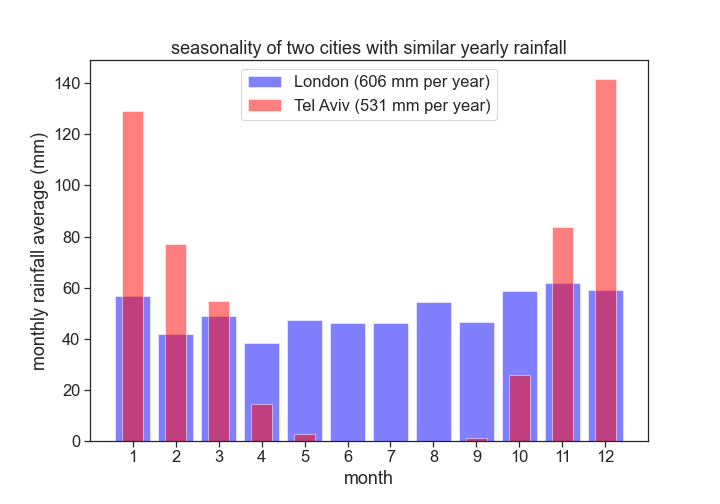
\includegraphics{archive/figures/monthly_tel_aviv_london_bars.png}

Let's shift the months according the the hydrological year:\\
\includegraphics{archive/figures/monthly_tel_aviv_london_bars_hydrological_year.png}

\includegraphics{archive/figures/radar_chart_tel_aviv_london.png}

Sources: leddris (2010), Walsh and Lawler (1981)

\(R=\) mean annual precipitation\\
\(m_i=\) precipitation mean for month \(i\)

\[ SI = \displaystyle \frac{1}{R} \sum_{n=1}^{n=12} \left| m_i - \frac{R}{12} \right| \]

\begin{longtable}[]{@{}
  >{\raggedright\arraybackslash}p{(\columnwidth - 2\tabcolsep) * \real{0.1500}}
  >{\raggedright\arraybackslash}p{(\columnwidth - 2\tabcolsep) * \real{0.8500}}@{}}
\toprule()
\begin{minipage}[b]{\linewidth}\raggedright
\(SI\)
\end{minipage} & \begin{minipage}[b]{\linewidth}\raggedright
Precipitation Regime
\end{minipage} \\
\midrule()
\endhead
\textless0.19 & Precipitation spread throughout the year \\
0.20-0.39 & Precipitation spread throughout the year, but with a
definite wetter season \\
0.40-0.59 & Rather seasonal with a short dry season \\
0.60-0.79 & Seasonal \\
0.80-0.99 & Marked seasonal with a long dry season \\
1.00-1.19 & Most precipitation in \textless3 months \\
\bottomrule()
\end{longtable}

Let's write some code to calculate the SI for Tel Aviv and London.

\begin{Shaded}
\begin{Highlighting}[]
\CommentTok{\# import packages}
\ImportTok{import}\NormalTok{ numpy }\ImportTok{as}\NormalTok{ np}
\ImportTok{import}\NormalTok{ pandas }\ImportTok{as}\NormalTok{ pd}
\ImportTok{from}\NormalTok{ calendar }\ImportTok{import}\NormalTok{ month\_abbr}

\CommentTok{\# load data}
\NormalTok{month\_numbers }\OperatorTok{=}\NormalTok{ np.arange(}\DecValTok{1}\NormalTok{,}\DecValTok{13}\NormalTok{)}
\NormalTok{month\_names }\OperatorTok{=}\NormalTok{ [month\_abbr[i] }\ControlFlowTok{for}\NormalTok{ i }\KeywordTok{in}\NormalTok{ month\_numbers]}
\KeywordTok{def}\NormalTok{ monthly\_mean(station\_name, freq):}
    \CommentTok{\# import daily data}
\NormalTok{    df }\OperatorTok{=}\NormalTok{ pd.read\_csv(station\_name }\OperatorTok{+} \StringTok{\textquotesingle{}\_\textquotesingle{}} \OperatorTok{+}\NormalTok{ freq }\OperatorTok{+} \StringTok{\textquotesingle{}.csv\textquotesingle{}}\NormalTok{, sep}\OperatorTok{=}\StringTok{","}\NormalTok{)}
    \CommentTok{\# make \textquotesingle{}DATE\textquotesingle{} the dataframe index}
\NormalTok{    df[}\StringTok{\textquotesingle{}DATE\textquotesingle{}}\NormalTok{] }\OperatorTok{=}\NormalTok{ pd.to\_datetime(df[}\StringTok{\textquotesingle{}DATE\textquotesingle{}}\NormalTok{])}
\NormalTok{    df }\OperatorTok{=}\NormalTok{ df.set\_index(}\StringTok{\textquotesingle{}DATE\textquotesingle{}}\NormalTok{)}
    \CommentTok{\# print(df.index[0], df.index[{-}1])}
    \ControlFlowTok{if}\NormalTok{ freq }\OperatorTok{==} \StringTok{\textquotesingle{}daily\textquotesingle{}}\NormalTok{:}
        \CommentTok{\# resample data by month}
\NormalTok{        df\_month }\OperatorTok{=}\NormalTok{ df[}\StringTok{\textquotesingle{}PRCP\textquotesingle{}}\NormalTok{].resample(}\StringTok{\textquotesingle{}M\textquotesingle{}}\NormalTok{).}\BuiltInTok{sum}\NormalTok{()  }\CommentTok{\# sum is labeled at the last day of the month }
\NormalTok{        df\_month }\OperatorTok{=}\NormalTok{ df\_month}\OperatorTok{/}\DecValTok{10}                     \CommentTok{\# PRCP is given in tens of mm (see readme)}
    \ControlFlowTok{if}\NormalTok{ freq }\OperatorTok{==} \StringTok{\textquotesingle{}monthly\textquotesingle{}}\NormalTok{:}
\NormalTok{        df\_month }\OperatorTok{=}\NormalTok{ df[}\StringTok{\textquotesingle{}PRCP\textquotesingle{}}\NormalTok{]}
    \CommentTok{\# calculate monthly mean}
\NormalTok{    monthly\_mean }\OperatorTok{=}\NormalTok{ np.array([])  }\CommentTok{\# empty array}
    \ControlFlowTok{for}\NormalTok{ m }\KeywordTok{in}\NormalTok{ month\_numbers:      }\CommentTok{\# cycle over months (1, 2, 3, etc)}
\NormalTok{        this\_month\_all\_indices }\OperatorTok{=}\NormalTok{ (df\_month.index.month }\OperatorTok{==}\NormalTok{ m)       }\CommentTok{\# indices in df\_month belonging to month m}
\NormalTok{        this\_month\_mean }\OperatorTok{=}\NormalTok{ df\_month[this\_month\_all\_indices].mean()  }\CommentTok{\# this is the monthly mean}
\NormalTok{        monthly\_mean }\OperatorTok{=}\NormalTok{ np.append(monthly\_mean, this\_month\_mean)    }\CommentTok{\# append}
    \CommentTok{\# make new df and return it}
\NormalTok{    df\_return }\OperatorTok{=}\NormalTok{ pd.DataFrame(\{}\StringTok{\textquotesingle{}monthly rainfall (mm)\textquotesingle{}}\NormalTok{:monthly\_mean,}
                              \StringTok{\textquotesingle{}month names\textquotesingle{}}\NormalTok{:month\_names,}
                              \StringTok{\textquotesingle{}month number\textquotesingle{}}\NormalTok{:month\_numbers}
\NormalTok{                            \})}
    \ControlFlowTok{return}\NormalTok{ df\_return}

\CommentTok{\# load monthly mean}
\NormalTok{df\_london }\OperatorTok{=}\NormalTok{ monthly\_mean(}\StringTok{"LONDON\_HEATHROW"}\NormalTok{, }\StringTok{\textquotesingle{}monthly\textquotesingle{}}\NormalTok{)}
\NormalTok{df\_telaviv }\OperatorTok{=}\NormalTok{ monthly\_mean(}\StringTok{"TEL\_AVIV\_READING"}\NormalTok{, }\StringTok{\textquotesingle{}monthly\textquotesingle{}}\NormalTok{)}
\end{Highlighting}
\end{Shaded}

\begin{Shaded}
\begin{Highlighting}[]
\KeywordTok{def}\NormalTok{ walsh\_index(df):}
\NormalTok{    m }\OperatorTok{=}\NormalTok{ df[}\StringTok{"monthly rainfall (mm)"}\NormalTok{]}
\NormalTok{    R }\OperatorTok{=}\NormalTok{ df[}\StringTok{"monthly rainfall (mm)"}\NormalTok{].}\BuiltInTok{sum}\NormalTok{()}
\NormalTok{    SI }\OperatorTok{=}\NormalTok{ np.}\BuiltInTok{sum}\NormalTok{(np.}\BuiltInTok{abs}\NormalTok{(m}\OperatorTok{{-}}\NormalTok{R}\OperatorTok{/}\DecValTok{12}\NormalTok{)) }\OperatorTok{/}\NormalTok{ R}
    \ControlFlowTok{return}\NormalTok{ SI}

\NormalTok{london\_index }\OperatorTok{=}\NormalTok{ walsh\_index(df\_london)}
\NormalTok{telaviv\_index }\OperatorTok{=}\NormalTok{ walsh\_index(df\_telaviv)}
\BuiltInTok{print}\NormalTok{(}\StringTok{"Seasonality index (Walsh and Lawler, 1981)"}\NormalTok{)}
\BuiltInTok{print}\NormalTok{(}\SpecialStringTok{f"London: }\SpecialCharTok{\{}\NormalTok{london\_index}\SpecialCharTok{:.2f\}}\SpecialStringTok{"}\NormalTok{)}
\BuiltInTok{print}\NormalTok{(}\SpecialStringTok{f"Tel Aviv: }\SpecialCharTok{\{}\NormalTok{telaviv\_index}\SpecialCharTok{:.2f\}}\SpecialStringTok{"}\NormalTok{)}
\end{Highlighting}
\end{Shaded}

\begin{verbatim}
Seasonality index (Walsh and Lawler, 1981)
London: 0.13
Tel Aviv: 1.00
\end{verbatim}

\hypertarget{exercises-2}{%
\chapter{Exercises}\label{exercises-2}}

Import relevant packages

\begin{Shaded}
\begin{Highlighting}[]
\ImportTok{import}\NormalTok{ matplotlib.pyplot }\ImportTok{as}\NormalTok{ plt}
\ImportTok{import}\NormalTok{ numpy }\ImportTok{as}\NormalTok{ np}
\ImportTok{import}\NormalTok{ pandas }\ImportTok{as}\NormalTok{ pd}
\ImportTok{from}\NormalTok{ calendar }\ImportTok{import}\NormalTok{ month\_abbr}
\ImportTok{import}\NormalTok{ seaborn }\ImportTok{as}\NormalTok{ sns}
\NormalTok{sns.}\BuiltInTok{set}\NormalTok{(style}\OperatorTok{=}\StringTok{"ticks"}\NormalTok{, font\_scale}\OperatorTok{=}\FloatTok{1.5}\NormalTok{)}
\ImportTok{import}\NormalTok{ urllib.request}
\ImportTok{from}\NormalTok{ pandas.plotting }\ImportTok{import}\NormalTok{ register\_matplotlib\_converters}
\NormalTok{register\_matplotlib\_converters()}
\end{Highlighting}
\end{Shaded}

\hypertarget{intra-annual-variability}{%
\section{intra-annual variability}\label{intra-annual-variability}}

Go to NOAA's National Centers for Environmental Information (NCEI)\\
\href{https://www.ncdc.noaa.gov/cdo-web/datasets}{Climate Data Online:
Dataset Discovery}

Find station codes in this
\href{https://www.ncei.noaa.gov/maps/monthly/}{map}. On the left, click
on the little wrench (🔧) next to ``Global Summary of the Month'', then
click on ``identify'' on the panel that just opened, and click on a
station (purple circle). You will see the station's name, it's ID, and
the period of record. For example, for Ben-Gurion's Airport in Israel:\\
BEN GURION, IS\\
STATION ID: ISM00040180\\
Period of Record: 1951-01-01 to 2020-03-01

You can download \textbf{daily} or \textbf{monthly} data for each
station. Use the function below to download this data to your computer.

\begin{Shaded}
\begin{Highlighting}[]
\KeywordTok{def}\NormalTok{ download\_data(station\_name, station\_code):}
\NormalTok{    url\_daily }\OperatorTok{=} \StringTok{\textquotesingle{}https://www.ncei.noaa.gov/data/global{-}historical{-}climatology{-}network{-}daily/access/\textquotesingle{}}
\NormalTok{    url\_monthly }\OperatorTok{=} \StringTok{\textquotesingle{}https://www.ncei.noaa.gov/data/gsom/access/\textquotesingle{}}
    \CommentTok{\# download daily data {-} uncomment the next 2 lines to make this work}
    \CommentTok{\# urllib.request.urlretrieve(url\_daily + station\_code + \textquotesingle{}.csv\textquotesingle{},}
    \CommentTok{\#                            station\_name + \textquotesingle{}\_daily.csv\textquotesingle{})}
    \CommentTok{\# download monthly data}
\NormalTok{    urllib.request.urlretrieve(url\_monthly }\OperatorTok{+}\NormalTok{ station\_code }\OperatorTok{+} \StringTok{\textquotesingle{}.csv\textquotesingle{}}\NormalTok{,}
\NormalTok{                               station\_name }\OperatorTok{+} \StringTok{\textquotesingle{}\_monthly.csv\textquotesingle{}}\NormalTok{)}
\end{Highlighting}
\end{Shaded}

Now, choose any station with a period of record longer than 30 years,
and download its data:

\begin{Shaded}
\begin{Highlighting}[]
\NormalTok{download\_data(}\StringTok{\textquotesingle{}BEN\_GURION\textquotesingle{}}\NormalTok{, }\StringTok{\textquotesingle{}ISM00040180\textquotesingle{}}\NormalTok{)}
\end{Highlighting}
\end{Shaded}

Load the data into a datafram, and before you continue with the
analysis, plot the rainfall data, to see how it looks like.

\begin{Shaded}
\begin{Highlighting}[]
\NormalTok{download\_data(}\StringTok{\textquotesingle{}BEN\_GURION\textquotesingle{}}\NormalTok{, }\StringTok{\textquotesingle{}ISM00040180\textquotesingle{}}\NormalTok{)}
\NormalTok{df }\OperatorTok{=}\NormalTok{ pd.read\_csv(}\StringTok{\textquotesingle{}BEN\_GURION\_monthly.csv\textquotesingle{}}\NormalTok{, sep}\OperatorTok{=}\StringTok{","}\NormalTok{)}
\CommentTok{\# make \textquotesingle{}DATE\textquotesingle{} the dataframe index}
\NormalTok{df[}\StringTok{\textquotesingle{}DATE\textquotesingle{}}\NormalTok{] }\OperatorTok{=}\NormalTok{ pd.to\_datetime(df[}\StringTok{\textquotesingle{}DATE\textquotesingle{}}\NormalTok{])}
\NormalTok{df }\OperatorTok{=}\NormalTok{ df.set\_index(}\StringTok{\textquotesingle{}DATE\textquotesingle{}}\NormalTok{)}
\NormalTok{plt.plot(df[}\StringTok{\textquotesingle{}PRCP\textquotesingle{}}\NormalTok{])}
\end{Highlighting}
\end{Shaded}

\begin{figure}[H]

{\centering \includegraphics{precipitation/intra-annual-exercises_files/figure-pdf/cell-4-output-1.png}

}

\end{figure}

It doesn't look great for Ben-Gurion airport, lots of missing data! You
might need to choose another station\ldots{} Download data for Beer
Sheva, ID \texttt{IS000051690}.

\begin{Shaded}
\begin{Highlighting}[]
\NormalTok{download\_data(}\StringTok{\textquotesingle{}BEER\_SHEVA\textquotesingle{}}\NormalTok{, }\StringTok{\textquotesingle{}IS000051690\textquotesingle{}}\NormalTok{)}
\NormalTok{df }\OperatorTok{=}\NormalTok{ pd.read\_csv(}\StringTok{\textquotesingle{}BEER\_SHEVA\_monthly.csv\textquotesingle{}}\NormalTok{, sep}\OperatorTok{=}\StringTok{","}\NormalTok{)}
\CommentTok{\# make \textquotesingle{}DATE\textquotesingle{} the dataframe index}
\NormalTok{df[}\StringTok{\textquotesingle{}DATE\textquotesingle{}}\NormalTok{] }\OperatorTok{=}\NormalTok{ pd.to\_datetime(df[}\StringTok{\textquotesingle{}DATE\textquotesingle{}}\NormalTok{])}
\NormalTok{df }\OperatorTok{=}\NormalTok{ df.set\_index(}\StringTok{\textquotesingle{}DATE\textquotesingle{}}\NormalTok{)}
\NormalTok{plt.plot(df[}\StringTok{\textquotesingle{}PRCP\textquotesingle{}}\NormalTok{])}
\end{Highlighting}
\end{Shaded}

\begin{figure}[H]

{\centering \includegraphics{precipitation/intra-annual-exercises_files/figure-pdf/cell-5-output-1.png}

}

\end{figure}

That's much better! We need to aggregate all data from each month, so we
can calculate monthly averages. How to do that?

\begin{Shaded}
\begin{Highlighting}[]
\CommentTok{\# choose only the precipitation column}
\NormalTok{df\_month }\OperatorTok{=}\NormalTok{ df[}\StringTok{\textquotesingle{}PRCP\textquotesingle{}}\NormalTok{]}
\CommentTok{\# calculate monthly mean}
\NormalTok{monthly\_mean }\OperatorTok{=}\NormalTok{ np.array([])  }\CommentTok{\# empty array}
\NormalTok{month\_numbers }\OperatorTok{=}\NormalTok{ np.arange(}\DecValTok{1}\NormalTok{,}\DecValTok{13}\NormalTok{)}
\NormalTok{month\_names }\OperatorTok{=}\NormalTok{ [month\_abbr[i] }\ControlFlowTok{for}\NormalTok{ i }\KeywordTok{in}\NormalTok{ month\_numbers]}

\ControlFlowTok{for}\NormalTok{ m }\KeywordTok{in}\NormalTok{ month\_numbers:      }\CommentTok{\# cycle over months (1, 2, 3, etc)}
\NormalTok{    this\_month\_all\_indices }\OperatorTok{=}\NormalTok{ (df\_month.index.month }\OperatorTok{==}\NormalTok{ m)       }\CommentTok{\# indices in df\_month belonging to month m}
\NormalTok{    this\_month\_mean }\OperatorTok{=}\NormalTok{ df\_month[this\_month\_all\_indices].mean()  }\CommentTok{\# this is the monthly mean}
\NormalTok{    monthly\_mean }\OperatorTok{=}\NormalTok{ np.append(monthly\_mean, this\_month\_mean)    }\CommentTok{\# append}
\end{Highlighting}
\end{Shaded}

Now it is time to create a new dataframe with the monthly means.

\begin{Shaded}
\begin{Highlighting}[]
\NormalTok{df\_beersheva }\OperatorTok{=}\NormalTok{ pd.DataFrame(\{}\StringTok{\textquotesingle{}monthly rainfall (mm)\textquotesingle{}}\NormalTok{:monthly\_mean,}
                             \StringTok{\textquotesingle{}month names\textquotesingle{}}\NormalTok{:month\_names,}
                             \StringTok{\textquotesingle{}month number\textquotesingle{}}\NormalTok{:month\_numbers}
\NormalTok{                            \})}
\NormalTok{df\_beersheva}
\end{Highlighting}
\end{Shaded}

\begin{longtable}[]{@{}llll@{}}
\toprule()
& monthly rainfall (mm) & month names & month number \\
\midrule()
\endhead
0 & 48.743158 & Jan & 1 \\
1 & 37.347368 & Feb & 2 \\
2 & 26.551579 & Mar & 3 \\
3 & 9.038947 & Apr & 4 \\
4 & 2.735789 & May & 5 \\
5 & 0.013830 & Jun & 6 \\
6 & 0.000000 & Jul & 7 \\
7 & 0.002128 & Aug & 8 \\
8 & 0.271277 & Sep & 9 \\
9 & 6.669474 & Oct & 10 \\
10 & 21.850526 & Nov & 11 \\
11 & 41.786316 & Dec & 12 \\
\bottomrule()
\end{longtable}

Plot the data and see if it makes sense. Try to get a figure like this
one.

\begin{Shaded}
\begin{Highlighting}[]
\NormalTok{fig, ax }\OperatorTok{=}\NormalTok{ plt.subplots(figsize}\OperatorTok{=}\NormalTok{(}\DecValTok{10}\NormalTok{,}\DecValTok{7}\NormalTok{))}
\NormalTok{ax.bar(df\_beersheva[}\StringTok{\textquotesingle{}month number\textquotesingle{}}\NormalTok{], df\_beersheva[}\StringTok{\textquotesingle{}monthly rainfall (mm)\textquotesingle{}}\NormalTok{])}
\NormalTok{ax.}\BuiltInTok{set}\NormalTok{(xlabel}\OperatorTok{=}\StringTok{"months"}\NormalTok{,}
\NormalTok{       ylabel}\OperatorTok{=}\StringTok{"monthly average (mm)"}\NormalTok{,}
\NormalTok{       title}\OperatorTok{=}\StringTok{"Beer Sheva"}\NormalTok{,}
\NormalTok{       xticks}\OperatorTok{=}\NormalTok{df\_beersheva[}\StringTok{\textquotesingle{}month number\textquotesingle{}}\NormalTok{],}
\NormalTok{       xticklabels}\OperatorTok{=}\NormalTok{df\_beersheva[}\StringTok{\textquotesingle{}month names\textquotesingle{}}\NormalTok{])}\OperatorTok{;}
\NormalTok{plt.savefig(}\StringTok{"hydrology\_figures/beersheva\_monthly\_average.png"}\NormalTok{)}
\end{Highlighting}
\end{Shaded}

\begin{figure}[H]

{\centering \includegraphics{precipitation/intra-annual-exercises_files/figure-pdf/cell-8-output-1.png}

}

\end{figure}

Let's calculate now the Walsh and Lawler Seasonality Index.\\
\textbf{Write a function} that receives a dataframe like the one we have
just created, and returns the seasonality index.\\
http://leddris.aegean.gr/ses-parameters/293-rainfall-seasonality.html\#:\textasciitilde:text=Rainfall\%20seasonality\%20index\%20is\%20a,in\%20relation\%20to\%20water\%20availability

\(R=\) mean annual precipitation\\
\(m_i\) precipitation mean for month \(i\)

\[ SI = \displaystyle \frac{1}{R} \sum_{n=1}^{n=12} \left| m_i - \frac{R}{12} \right| \]

\begin{longtable}[]{@{}
  >{\raggedright\arraybackslash}p{(\columnwidth - 2\tabcolsep) * \real{0.5000}}
  >{\raggedright\arraybackslash}p{(\columnwidth - 2\tabcolsep) * \real{0.5000}}@{}}
\toprule()
\begin{minipage}[b]{\linewidth}\raggedright
SI
\end{minipage} & \begin{minipage}[b]{\linewidth}\raggedright
Precipitation Regime
\end{minipage} \\
\midrule()
\endhead
\textless0.19 & Precipitation spread throughout the year \\
0.20-0.39 & Precipitation spread throughout the year, but with a
definite wetter season \\
0.40-0.59 & Rather seasonal with a short dry season \\
0.60-0.79 & Seasonal \\
0.80-0.99 & Marked seasonal with a long dry season \\
1.00-1.19 & Most precipitation in \textless{} 3 months \\
\bottomrule()
\end{longtable}

\begin{Shaded}
\begin{Highlighting}[]
\KeywordTok{def}\NormalTok{ walsh\_index(df):}
\NormalTok{    mi }\OperatorTok{=}\NormalTok{ df[}\StringTok{"monthly rainfall (mm)"}\NormalTok{]}
\NormalTok{    R }\OperatorTok{=}\NormalTok{ df[}\StringTok{"monthly rainfall (mm)"}\NormalTok{].}\BuiltInTok{sum}\NormalTok{()}
\NormalTok{    SI }\OperatorTok{=}\NormalTok{ np.}\BuiltInTok{sum}\NormalTok{(np.}\BuiltInTok{abs}\NormalTok{(mi }\OperatorTok{{-}}\NormalTok{ R}\OperatorTok{/}\DecValTok{12}\NormalTok{)) }\OperatorTok{/}\NormalTok{ R}
    \ControlFlowTok{return}\NormalTok{ SI}
\NormalTok{beersheva\_SI }\OperatorTok{=}\NormalTok{ walsh\_index(df\_beersheva)}
\BuiltInTok{print}\NormalTok{(}\SpecialStringTok{f"Beer Sheva, SI = }\SpecialCharTok{\{}\NormalTok{beersheva\_SI}\SpecialCharTok{:.2f\}}\SpecialStringTok{"}\NormalTok{)}
\end{Highlighting}
\end{Shaded}

\begin{verbatim}
Beer Sheva, SI = 0.97
\end{verbatim}

\hypertarget{return-period}{%
\chapter{Return Period}\label{return-period}}

\includegraphics{archive/figures/bilbao-map.png}

\hypertarget{today}{%
\section{Today}\label{today}}

\includegraphics{https://upload.wikimedia.org/wikipedia/commons/9/90/Guggenheim_museum_Bilbao_HDR-image.jpg}

\hypertarget{august-1983}{%
\section{August 1983}\label{august-1983}}

\includegraphics{archive/figures/bilbao-flood-cars.jpg}

On Friday, August 26, 1983, Bilbao was celebrating its Aste Nagusia or
Great Week, the main annual festivity in the city, when it and other
municipalities of the Basque Country, Burgos, and Cantabria suffered
devastating flooding due to heavy rains. In 24 hours, the volume of
water registered 600 liters per square meter. Across all the affected
areas, the weather service recorded 1.5 billion tons of water. In areas
of Bilbao, the water reached a height of 5 meters (15 feet).
Transportation, electricity and gas services, drinking water, food,
telephone, and many other basic services were severely affected. 32
people died in Biscay, 4 people died in Cantabria, 2 people died in
Alava, and 2 people died Burgos. 5 more people went missing.

\hypertarget{how-often-will-such-rainfall-happen}{%
\section{How often will such rainfall
happen?}\label{how-often-will-such-rainfall-happen}}

How often does it rain 50 mm in 1 day? What about 100 mm in 1 day? How
big is a ``once-in-a-century event''?

Let's examine Bilbao's daily rainfall (mm), between 1947 to 2021

\includegraphics{archive/figures/bilbao-1947-2021.png}

On the week of 22-28 August 1983, Bilbao's weather station measured 4.5
m of rainfall!

\includegraphics{archive/figures/bilbao-august-1983.png}

Let's analyze this data and find out how rare such events are. First we
need to find the annual maximum for each hydrological year.

\begin{Shaded}
\begin{Highlighting}[]
\ImportTok{import}\NormalTok{ matplotlib.pyplot }\ImportTok{as}\NormalTok{ plt}
\ImportTok{import}\NormalTok{ numpy }\ImportTok{as}\NormalTok{ np}
\ImportTok{import}\NormalTok{ pandas }\ImportTok{as}\NormalTok{ pd}

\NormalTok{df }\OperatorTok{=}\NormalTok{ pd.read\_csv(}\StringTok{\textquotesingle{}BILBAO\_daily.csv\textquotesingle{}}\NormalTok{, sep}\OperatorTok{=}\StringTok{","}\NormalTok{)}
\NormalTok{df[}\StringTok{\textquotesingle{}DATE\textquotesingle{}}\NormalTok{] }\OperatorTok{=}\NormalTok{ pd.to\_datetime(df[}\StringTok{\textquotesingle{}DATE\textquotesingle{}}\NormalTok{])}
\NormalTok{df }\OperatorTok{=}\NormalTok{ df.set\_index(}\StringTok{\textquotesingle{}DATE\textquotesingle{}}\NormalTok{)}
\CommentTok{\# IMPORTANT!! daily precipitation data is in tenths of mm, divide by 10 to get it in mm.}
\NormalTok{df[}\StringTok{\textquotesingle{}PRCP\textquotesingle{}}\NormalTok{] }\OperatorTok{=}\NormalTok{ df[}\StringTok{\textquotesingle{}PRCP\textquotesingle{}}\NormalTok{] }\OperatorTok{/} \DecValTok{10}

\ImportTok{import}\NormalTok{ altair }\ImportTok{as}\NormalTok{ alt}
\NormalTok{alt.data\_transformers.disable\_max\_rows()}

\CommentTok{\# Altair only recognizes column data; it ignores index values.}
\CommentTok{\# You can plot the index data by first resetting the index}
\CommentTok{\# I know that I\textquotesingle{}ve just made \textquotesingle{}DATE\textquotesingle{} the index, but I want to have this here nonetheless so I can refer to this in the future}
\NormalTok{df\_new }\OperatorTok{=}\NormalTok{ df.reset\_index()}\CommentTok{\#.replace(\{0.0:np.nan\})}
\NormalTok{source }\OperatorTok{=}\NormalTok{ df\_new[[}\StringTok{\textquotesingle{}DATE\textquotesingle{}}\NormalTok{, }\StringTok{\textquotesingle{}PRCP\textquotesingle{}}\NormalTok{]]}

\NormalTok{brush }\OperatorTok{=}\NormalTok{ alt.selection(}\BuiltInTok{type}\OperatorTok{=}\StringTok{\textquotesingle{}interval\textquotesingle{}}\NormalTok{, encodings}\OperatorTok{=}\NormalTok{[}\StringTok{\textquotesingle{}x\textquotesingle{}}\NormalTok{])}

\NormalTok{base }\OperatorTok{=}\NormalTok{ alt.Chart(source).mark\_line().encode(}
\NormalTok{    x }\OperatorTok{=} \StringTok{\textquotesingle{}DATE:T\textquotesingle{}}\NormalTok{,}
\NormalTok{    y }\OperatorTok{=} \StringTok{\textquotesingle{}PRCP:Q\textquotesingle{}}
\NormalTok{).properties(}
\NormalTok{    width}\OperatorTok{=}\DecValTok{600}\NormalTok{,}
\NormalTok{    height}\OperatorTok{=}\DecValTok{200}
\NormalTok{)}

\NormalTok{upper }\OperatorTok{=}\NormalTok{ base.encode(}
\NormalTok{    alt.X(}\StringTok{\textquotesingle{}DATE:T\textquotesingle{}}\NormalTok{, scale}\OperatorTok{=}\NormalTok{alt.Scale(domain}\OperatorTok{=}\NormalTok{brush)),}
\NormalTok{    alt.Y(}\StringTok{\textquotesingle{}PRCP:Q\textquotesingle{}}\NormalTok{, scale}\OperatorTok{=}\NormalTok{alt.Scale(domain}\OperatorTok{=}\NormalTok{(}\DecValTok{0}\NormalTok{,}\DecValTok{100}\NormalTok{)))}
\NormalTok{)}

\NormalTok{lower }\OperatorTok{=}\NormalTok{ base.properties(}
\NormalTok{    height}\OperatorTok{=}\DecValTok{60}
\NormalTok{).add\_selection(brush)}

\NormalTok{alt.vconcat(upper, lower)}
\end{Highlighting}
\end{Shaded}

\begin{verbatim}
alt.VConcatChart(...)
\end{verbatim}

We will consider a hydrological year starting on 1 August.
\includegraphics{archive/figures/monthly_average_bilbao.png}

Histogram of annual maximum events
\includegraphics{archive/figures/hist_count_cumulative_bilbao.png}

\includegraphics{archive/figures/pdf_cdf_bilbao.png}

How many years, \textbf{on average}, do we have to wait to get an annual
maximum above a given threshold?

\includegraphics{archive/figures/return_prob_050.png}

\includegraphics{archive/figures/return_prob_033.png}

\includegraphics{archive/figures/return_prob_020.png}

\includegraphics{archive/figures/return_prob_010.png}

\includegraphics{archive/figures/return_prob_005.png}

Now everything together in one gif:

\includegraphics{archive/figures/return_prob.gif}

\hypertarget{return-period-1}{%
\section{Return Period}\label{return-period-1}}

We will follow Brutsaert (2005), page 513. He defines quantities a
little different from what we did above.

\(F(x)\) is the CDF of the PDF \(f(x)\). \(F(x)\) indicates the
non-exceedance probability, i.e., the probability that a certain event
above \(x\) has \textbf{not} occurred (or that an event below \(x\) has
occurred, same thing). Modifying the graph shown above, we have

\includegraphics{archive/figures/return_prob_050_reversed.png}

\(1-F(x)\) is the probability that a certain event above \(x\)
\emph{has} occurred. It's reciprocal is the return period:

\[
T_r(x) = \frac{1}{1-F(x)}
\]

This return period is the expected number of observations required until
\(x\) is exceeded once. In our case, we can ask the question: how many
years will pass (on average) until we see a rainfall event greater that
that of 26 August 1983?

Let's call \(p=F(x)\) the probability that we measured once and that an
event greater than \(x\) has \emph{not} occurred. What is the
probability that a rainfall above \(x\) will occur only on year number
\(k\)?\\
* it hasn't occurred on year 1 (probability p) * it hasn't occurred on
year 2 (probability p) * it hasn't occurred on year 3 (probability p) *
\ldots{} * it has occurred on year k (probability 1-p)

\(P\{k \text{ trials until }X>x\} = p^{k-1}(1-p)\)

Every time the number \(k\) will be different. What will be \(k\)
\emph{on average}?

\[\bar{k} = \displaystyle\sum_{k=1}^{\infty} k P(k) = \displaystyle\sum_{k=1}^{\infty} k p^{k-1}(1-p)\]

Let's open that up:

\[
\begin{align}
\bar{k} &= 1-p + 2p(1-p) + 3p^2(1-p) + 4p^3(1-p)+ \cdots\\
\bar{k} &= 1-p + 2p - 2p^2 + 3p^2 - 3p^4 + 4p^3 - 4p^4+ \cdots \\
\bar{k} &= 1 + p + p^2 + p^3 + p^4 + \cdots
\end{align}
\]

For \(p<1\), the series converges to \[
1 + p + p^2 + p^3 + p^4 + \cdots = \frac{1}{1-p},
\] therefore \[
\bar{k} = \frac{1}{1-p}.
\]

We conclude that if we know the exceedance probability, we immediately
can say what the return times are. We now need a way of estimating this
exceedance probability.

\hypertarget{plotting-position}{%
\section{Plotting Position}\label{plotting-position}}

Source: Brutsaert (2005), pages 514-516

The \textbf{Plotting Position} is used as an estimate of the exceedance
probability. Many formulas have been suggested (see source above), we
will use the \textbf{Weibull plotting position}:

\(P_m=\) plotting position, or probability of occurence for each event\\
\(n=\) total number of events\\
\(m=\) rank of each event, where \(m=1\) is the lowest value, and
\(m=n\) is the highest

\hypertarget{return-period-2}{%
\subsection{Return period}\label{return-period-2}}

\[
\text{Return period} = T_r = \frac{1}{1-P_m}
\]

\hypertarget{weibull-plotting-position}{%
\subsubsection{Weibull plotting
position:}\label{weibull-plotting-position}}

\[
P_m = \frac{m}{n+1}
\]

Now let's calculate that for Bilbao:

\begin{Shaded}
\begin{Highlighting}[]
\CommentTok{\# resample daily data into yearly data (maximum yearly value)}
\NormalTok{max\_annual }\OperatorTok{=}\NormalTok{ df[}\StringTok{\textquotesingle{}PRCP\textquotesingle{}}\NormalTok{].resample(}\StringTok{\textquotesingle{}A{-}JUL\textquotesingle{}}\NormalTok{).}\BuiltInTok{max}\NormalTok{().to\_frame()}
\CommentTok{\# sort yearly max from lowest to highest}
\NormalTok{max\_annual }\OperatorTok{=}\NormalTok{ max\_annual.sort\_values(by}\OperatorTok{=}\NormalTok{[}\StringTok{\textquotesingle{}PRCP\textquotesingle{}}\NormalTok{], ascending}\OperatorTok{=}\VariableTok{True}\NormalTok{)}
\NormalTok{max\_annual[}\StringTok{\textquotesingle{}m\textquotesingle{}}\NormalTok{] }\OperatorTok{=}\NormalTok{ np.arange(}\DecValTok{1}\NormalTok{, }\BuiltInTok{len}\NormalTok{(max\_annual) }\OperatorTok{+} \DecValTok{1}\NormalTok{)}
\NormalTok{n }\OperatorTok{=} \BuiltInTok{len}\NormalTok{(max\_annual[}\StringTok{\textquotesingle{}m\textquotesingle{}}\NormalTok{])}
\NormalTok{max\_annual[}\StringTok{\textquotesingle{}Pm\textquotesingle{}}\NormalTok{] }\OperatorTok{=}\NormalTok{ max\_annual[}\StringTok{\textquotesingle{}m\textquotesingle{}}\NormalTok{] }\OperatorTok{/}\NormalTok{ (n}\OperatorTok{+}\DecValTok{1}\NormalTok{)}
\NormalTok{max\_annual[}\StringTok{\textquotesingle{}Tr\textquotesingle{}}\NormalTok{] }\OperatorTok{=} \DecValTok{1} \OperatorTok{/}\NormalTok{ (}\DecValTok{1} \OperatorTok{{-}}\NormalTok{ max\_annual[}\StringTok{\textquotesingle{}Pm\textquotesingle{}}\NormalTok{])}
\NormalTok{max\_annual}
\end{Highlighting}
\end{Shaded}

\begin{tabular}{lrrrr}
\toprule
{} &   PRCP &   m &        Pm &         Tr \\
DATE       &        &     &           &            \\
\midrule
2011-07-31 &   27.0 &   1 &  0.013158 &   1.013333 \\
2002-07-31 &   28.5 &   2 &  0.026316 &   1.027027 \\
2021-07-31 &   35.8 &   3 &  0.039474 &   1.041096 \\
2001-07-31 &   38.6 &   4 &  0.052632 &   1.055556 \\
2004-07-31 &   41.1 &   5 &  0.065789 &   1.070423 \\
1998-07-31 &   41.3 &   6 &  0.078947 &   1.085714 \\
1948-07-31 &   41.8 &   7 &  0.092105 &   1.101449 \\
2019-07-31 &   42.3 &   8 &  0.105263 &   1.117647 \\
2018-07-31 &   44.6 &   9 &  0.118421 &   1.134328 \\
1965-07-31 &   45.1 &  10 &  0.131579 &   1.151515 \\
1995-07-31 &   45.2 &  11 &  0.144737 &   1.169231 \\
2005-07-31 &   45.6 &  12 &  0.157895 &   1.187500 \\
1970-07-31 &   46.4 &  13 &  0.171053 &   1.206349 \\
1990-07-31 &   46.4 &  14 &  0.184211 &   1.225806 \\
2000-07-31 &   46.4 &  15 &  0.197368 &   1.245902 \\
1967-07-31 &   46.5 &  16 &  0.210526 &   1.266667 \\
1962-07-31 &   47.7 &  17 &  0.223684 &   1.288136 \\
1957-07-31 &   47.8 &  18 &  0.236842 &   1.310345 \\
1988-07-31 &   48.9 &  19 &  0.250000 &   1.333333 \\
2014-07-31 &   49.9 &  20 &  0.263158 &   1.357143 \\
1958-07-31 &   50.2 &  21 &  0.276316 &   1.381818 \\
1973-07-31 &   50.7 &  22 &  0.289474 &   1.407407 \\
1956-07-31 &   51.0 &  23 &  0.302632 &   1.433962 \\
1976-07-31 &   51.1 &  24 &  0.315789 &   1.461538 \\
1983-07-31 &   51.4 &  25 &  0.328947 &   1.490196 \\
1972-07-31 &   51.8 &  26 &  0.342105 &   1.520000 \\
1979-07-31 &   52.3 &  27 &  0.355263 &   1.551020 \\
1987-07-31 &   52.4 &  28 &  0.368421 &   1.583333 \\
2006-07-31 &   52.6 &  29 &  0.381579 &   1.617021 \\
1981-07-31 &   53.0 &  30 &  0.394737 &   1.652174 \\
1959-07-31 &   53.0 &  31 &  0.407895 &   1.688889 \\
2020-07-31 &   53.1 &  32 &  0.421053 &   1.727273 \\
1996-07-31 &   53.5 &  33 &  0.434211 &   1.767442 \\
1986-07-31 &   53.7 &  34 &  0.447368 &   1.809524 \\
2009-07-31 &   55.4 &  35 &  0.460526 &   1.853659 \\
1982-07-31 &   55.9 &  36 &  0.473684 &   1.900000 \\
1994-07-31 &   56.0 &  37 &  0.486842 &   1.948718 \\
1974-07-31 &   56.3 &  38 &  0.500000 &   2.000000 \\
1947-07-31 &   57.6 &  39 &  0.513158 &   2.054054 \\
2013-07-31 &   57.7 &  40 &  0.526316 &   2.111111 \\
1949-07-31 &   58.8 &  41 &  0.539474 &   2.171429 \\
1975-07-31 &   58.8 &  42 &  0.552632 &   2.235294 \\
1963-07-31 &   58.8 &  43 &  0.565789 &   2.303030 \\
1969-07-31 &   59.0 &  44 &  0.578947 &   2.375000 \\
1953-07-31 &   59.8 &  45 &  0.592105 &   2.451613 \\
1980-07-31 &   61.6 &  46 &  0.605263 &   2.533333 \\
1951-07-31 &   61.7 &  47 &  0.618421 &   2.620690 \\
1950-07-31 &   61.8 &  48 &  0.631579 &   2.714286 \\
1978-07-31 &   62.4 &  49 &  0.644737 &   2.814815 \\
2003-07-31 &   62.6 &  50 &  0.657895 &   2.923077 \\
1971-07-31 &   63.7 &  51 &  0.671053 &   3.040000 \\
1955-07-31 &   64.5 &  52 &  0.684211 &   3.166667 \\
2017-07-31 &   65.6 &  53 &  0.697368 &   3.304348 \\
1999-07-31 &   65.7 &  54 &  0.710526 &   3.454545 \\
1985-07-31 &   67.3 &  55 &  0.723684 &   3.619048 \\
1966-07-31 &   67.4 &  56 &  0.736842 &   3.800000 \\
1997-07-31 &   67.7 &  57 &  0.750000 &   4.000000 \\
1968-07-31 &   68.0 &  58 &  0.763158 &   4.222222 \\
1992-07-31 &   68.6 &  59 &  0.776316 &   4.470588 \\
2016-07-31 &   79.8 &  60 &  0.789474 &   4.750000 \\
2012-07-31 &   81.1 &  61 &  0.802632 &   5.066667 \\
2015-07-31 &   82.1 &  62 &  0.815789 &   5.428571 \\
1952-07-31 &   82.6 &  63 &  0.828947 &   5.846154 \\
1991-07-31 &   83.8 &  64 &  0.842105 &   6.333333 \\
1993-07-31 &   84.6 &  65 &  0.855263 &   6.909091 \\
2007-07-31 &   85.2 &  66 &  0.868421 &   7.600000 \\
1961-07-31 &   87.3 &  67 &  0.881579 &   8.444444 \\
1989-07-31 &   92.4 &  68 &  0.894737 &   9.500000 \\
2008-07-31 &   92.5 &  69 &  0.907895 &  10.857143 \\
1977-07-31 &  100.2 &  70 &  0.921053 &  12.666667 \\
2010-07-31 &  108.1 &  71 &  0.934211 &  15.200000 \\
1960-07-31 &  137.2 &  72 &  0.947368 &  19.000000 \\
1964-07-31 &  143.5 &  73 &  0.960526 &  25.333333 \\
1954-07-31 &  172.6 &  74 &  0.973684 &  38.000000 \\
1984-07-31 &  252.6 &  75 &  0.986842 &  76.000000 \\
\bottomrule
\end{tabular}

How well does \(P_m\) approximate \(F(x)\)?

\includegraphics{archive/figures/weibull_plotting_position.png}

We can now see in this graph how long it takes, \textbf{on average}, for
an annual maximum event above any threshold.

\includegraphics{archive/figures/annual_max_vs_return_period.png}

For times longer than \(n\), we need to extrapolate from the curve
above.

\includegraphics{archive/figures/extrapolation_exceedance1.png}

\includegraphics{archive/figures/extrapolation_exceedance2.png}

\includegraphics{archive/figures/extrapolation_exceedance3.png}

\includegraphics{archive/figures/extrapolation_exceedance4.png}

\hypertarget{exercises-3}{%
\chapter{Exercises}\label{exercises-3}}

Import relevant packages

\begin{Shaded}
\begin{Highlighting}[]
\ImportTok{import}\NormalTok{ matplotlib.pyplot }\ImportTok{as}\NormalTok{ plt}
\ImportTok{import}\NormalTok{ numpy }\ImportTok{as}\NormalTok{ np}
\ImportTok{import}\NormalTok{ pandas }\ImportTok{as}\NormalTok{ pd}
\ImportTok{from}\NormalTok{ functools }\ImportTok{import} \BuiltInTok{reduce}
\ImportTok{import}\NormalTok{ re}
\ImportTok{import}\NormalTok{ probscale}
\ImportTok{import}\NormalTok{ seaborn }\ImportTok{as}\NormalTok{ sns}
\NormalTok{sns.}\BuiltInTok{set}\NormalTok{(style}\OperatorTok{=}\StringTok{"ticks"}\NormalTok{, font\_scale}\OperatorTok{=}\FloatTok{1.5}\NormalTok{)}
\ImportTok{from}\NormalTok{ pandas.plotting }\ImportTok{import}\NormalTok{ register\_matplotlib\_converters}
\NormalTok{register\_matplotlib\_converters()}
\ImportTok{import}\NormalTok{ urllib.request}
\end{Highlighting}
\end{Shaded}

Go to NOAA's National Centers for Environmental Information (NCEI)\\
\href{https://www.ncdc.noaa.gov/cdo-web/datasets}{Climate Data Online:
Dataset Discovery}

Find station codes in this
\href{https://gis.ncdc.noaa.gov/maps/ncei/cdo/monthly}{map}. On the
left, click on the little wrench next to ``Global Summary of the
Month'', then click on ``identify'' on the panel that just opened, and
click on a station (purple circle). You will see the station's name,
it's ID, and the period of record. For example, for Ben-Gurion's Airport
in Israel:\\
BEN GURION, IS\\
STATION ID: ISM00040180\\
Period of Record: 1951-01-01 to 2020-03-01

You can download \textbf{daily} or \textbf{monthly} data for each
station. Use the function below to download this data to your computer.
\texttt{station\_name} can be whatever you want, \texttt{station\_code}
is the station ID.

\begin{Shaded}
\begin{Highlighting}[]
\KeywordTok{def}\NormalTok{ download\_data(station\_name, station\_code):}
\NormalTok{    url\_daily }\OperatorTok{=} \StringTok{\textquotesingle{}https://www.ncei.noaa.gov/data/global{-}historical{-}climatology{-}network{-}daily/access/\textquotesingle{}}
\NormalTok{    url\_monthly }\OperatorTok{=} \StringTok{\textquotesingle{}https://www.ncei.noaa.gov/data/gsom/access/\textquotesingle{}}
    \CommentTok{\# download daily data {-} uncomment the following 2 lines to make this work}
    \CommentTok{\# urllib.request.urlretrieve(url\_daily + station\_code + \textquotesingle{}.csv\textquotesingle{},}
    \CommentTok{\#                           station\_name + \textquotesingle{}\_daily.csv\textquotesingle{})}
    \CommentTok{\# download monthly data}
\NormalTok{    urllib.request.urlretrieve(url\_monthly }\OperatorTok{+}\NormalTok{ station\_code }\OperatorTok{+} \StringTok{\textquotesingle{}.csv\textquotesingle{}}\NormalTok{,}
\NormalTok{                               station\_name }\OperatorTok{+} \StringTok{\textquotesingle{}\_monthly.csv\textquotesingle{}}\NormalTok{)}
\end{Highlighting}
\end{Shaded}

Download daily rainfall data for Eilat, Israel. ID: IS000009972

\begin{Shaded}
\begin{Highlighting}[]
\NormalTok{download\_data(}\StringTok{\textquotesingle{}Eilat\textquotesingle{}}\NormalTok{, }\StringTok{\textquotesingle{}IS000009972\textquotesingle{}}\NormalTok{)}
\end{Highlighting}
\end{Shaded}

Then load the data into a dataframe.\\
\textbf{IMPORTANT!!} daily precipitation data is in tenths of mm, divide
by 10 to get it in mm.

\begin{Shaded}
\begin{Highlighting}[]
\NormalTok{df }\OperatorTok{=}\NormalTok{ pd.read\_csv(}\StringTok{\textquotesingle{}Eilat\_daily.csv\textquotesingle{}}\NormalTok{, sep}\OperatorTok{=}\StringTok{","}\NormalTok{)}
\CommentTok{\# make \textquotesingle{}DATE\textquotesingle{} the dataframe index}
\NormalTok{df[}\StringTok{\textquotesingle{}DATE\textquotesingle{}}\NormalTok{] }\OperatorTok{=}\NormalTok{ pd.to\_datetime(df[}\StringTok{\textquotesingle{}DATE\textquotesingle{}}\NormalTok{])}
\NormalTok{df }\OperatorTok{=}\NormalTok{ df.set\_index(}\StringTok{\textquotesingle{}DATE\textquotesingle{}}\NormalTok{)}
\CommentTok{\# IMPORTANT!! daily precipitation data is in tenths of mm, divide by 10 to get it in mm.}
\NormalTok{df[}\StringTok{\textquotesingle{}PRCP\textquotesingle{}}\NormalTok{] }\OperatorTok{=}\NormalTok{ df[}\StringTok{\textquotesingle{}PRCP\textquotesingle{}}\NormalTok{] }\OperatorTok{/} \DecValTok{10}
\NormalTok{df}
\end{Highlighting}
\end{Shaded}

\begin{longtable}[]{@{}llllllllllllll@{}}
\toprule()
& STATION & LATITUDE & LONGITUDE & ELEVATION & NAME & PRCP &
PRCP\_ATTRIBUTES & TMAX & TMAX\_ATTRIBUTES & TMIN & TMIN\_ATTRIBUTES &
TAVG & TAVG\_ATTRIBUTES \\
DATE & & & & & & & & & & & & & \\
\midrule()
\endhead
1949-11-30 & IS000009972 & 29.55 & 34.95 & 12.0 & ELAT, IS & 0.0 & ,,E &
NaN & NaN & NaN & NaN & NaN & NaN \\
1949-12-01 & IS000009972 & 29.55 & 34.95 & 12.0 & ELAT, IS & 0.0 & ,,E &
NaN & NaN & NaN & NaN & NaN & NaN \\
1949-12-02 & IS000009972 & 29.55 & 34.95 & 12.0 & ELAT, IS & 0.0 & ,,E &
NaN & NaN & NaN & NaN & NaN & NaN \\
1949-12-03 & IS000009972 & 29.55 & 34.95 & 12.0 & ELAT, IS & 0.0 & ,,E &
NaN & NaN & NaN & NaN & NaN & NaN \\
1949-12-04 & IS000009972 & 29.55 & 34.95 & 12.0 & ELAT, IS & 0.0 & ,,E &
NaN & NaN & NaN & NaN & NaN & NaN \\
... & ... & ... & ... & ... & ... & ... & ... & ... & ... & ... & ... &
... & ... \\
2021-03-24 & IS000009972 & 29.55 & 34.95 & 12.0 & ELAT, IS & 0.0 & ,,S &
287.0 & ,,S & NaN & NaN & 227.0 & H,,S \\
2021-03-25 & IS000009972 & 29.55 & 34.95 & 12.0 & ELAT, IS & NaN & NaN &
253.0 & ,,S & 154.0 & ,,S & 202.0 & H,,S \\
2021-03-26 & IS000009972 & 29.55 & 34.95 & 12.0 & ELAT, IS & NaN & NaN &
251.0 & ,,S & 134.0 & ,,S & 186.0 & H,,S \\
2021-03-27 & IS000009972 & 29.55 & 34.95 & 12.0 & ELAT, IS & NaN & NaN &
222.0 & ,,S & 119.0 & ,,S & 173.0 & H,,S \\
2021-03-28 & IS000009972 & 29.55 & 34.95 & 12.0 & ELAT, IS & NaN & NaN &
238.0 & ,,S & 119.0 & ,,S & 188.0 & H,,S \\
\bottomrule()
\end{longtable}

Plot precipitation data (`PRCP' column) and see if everything is all
right.

\begin{Shaded}
\begin{Highlighting}[]
\NormalTok{fig, ax }\OperatorTok{=}\NormalTok{ plt.subplots(figsize}\OperatorTok{=}\NormalTok{(}\DecValTok{10}\NormalTok{,}\DecValTok{7}\NormalTok{))}
\NormalTok{ax.plot(df[}\StringTok{\textquotesingle{}PRCP\textquotesingle{}}\NormalTok{])}
\NormalTok{ax.set\_xlabel(}\StringTok{"date"}\NormalTok{)}
\NormalTok{ax.set\_ylabel(}\StringTok{"daily rainfall (mm)"}\NormalTok{)}
\NormalTok{ax.set\_title(}\StringTok{"Eilat, 1949–2021"}\NormalTok{)}
\end{Highlighting}
\end{Shaded}

\begin{verbatim}
Text(0.5, 1.0, 'Eilat, 1949–2021')
\end{verbatim}

\begin{figure}[H]

{\centering \includegraphics{precipitation/return-period-exercises_files/figure-pdf/cell-6-output-2.png}

}

\end{figure}

Based on what you see, you might want to exclude certain periods, e.g.:

\begin{Shaded}
\begin{Highlighting}[]
\NormalTok{last\_date }\OperatorTok{=} \StringTok{\textquotesingle{}2018{-}08{-}01\textquotesingle{}}
\NormalTok{first\_date }\OperatorTok{=} \StringTok{\textquotesingle{}1950{-}08{-}01\textquotesingle{}}
\NormalTok{df }\OperatorTok{=}\NormalTok{ df[((df.index }\OperatorTok{\textless{}}\NormalTok{ last\_date) }\OperatorTok{\&}\NormalTok{ (df.index }\OperatorTok{\textgreater{}}\NormalTok{ first\_date))]}
\NormalTok{df}
\end{Highlighting}
\end{Shaded}

\begin{longtable}[]{@{}llllllllllllll@{}}
\toprule()
& STATION & LATITUDE & LONGITUDE & ELEVATION & NAME & PRCP &
PRCP\_ATTRIBUTES & TMAX & TMAX\_ATTRIBUTES & TMIN & TMIN\_ATTRIBUTES &
TAVG & TAVG\_ATTRIBUTES \\
DATE & & & & & & & & & & & & & \\
\midrule()
\endhead
1950-08-02 & IS000009972 & 29.55 & 34.95 & 12.0 & ELAT, IS & 0.0 & ,,E &
400.0 & ,,G & 240.0 & ,,G & NaN & NaN \\
1950-08-03 & IS000009972 & 29.55 & 34.95 & 12.0 & ELAT, IS & 0.0 & ,,E &
410.0 & ,,G & 260.0 & ,,G & NaN & NaN \\
1950-08-04 & IS000009972 & 29.55 & 34.95 & 12.0 & ELAT, IS & 0.0 & ,,E &
400.0 & ,,G & 260.0 & ,,G & NaN & NaN \\
1950-08-05 & IS000009972 & 29.55 & 34.95 & 12.0 & ELAT, IS & 0.0 & ,,E &
NaN & NaN & 240.0 & ,,G & NaN & NaN \\
1950-08-06 & IS000009972 & 29.55 & 34.95 & 12.0 & ELAT, IS & 0.0 & ,,E &
370.0 & ,,G & 240.0 & ,,G & NaN & NaN \\
... & ... & ... & ... & ... & ... & ... & ... & ... & ... & ... & ... &
... & ... \\
2018-07-27 & IS000009972 & 29.55 & 34.95 & 12.0 & ELAT, IS & 0.0 & ,,S &
414.0 & ,,S & NaN & NaN & 359.0 & H,,S \\
2018-07-28 & IS000009972 & 29.55 & 34.95 & 12.0 & ELAT, IS & 0.0 & ,,S &
386.0 & ,,S & NaN & NaN & 329.0 & H,,S \\
2018-07-29 & IS000009972 & 29.55 & 34.95 & 12.0 & ELAT, IS & 0.0 & ,,S &
NaN & NaN & 268.0 & ,,S & 334.0 & H,,S \\
2018-07-30 & IS000009972 & 29.55 & 34.95 & 12.0 & ELAT, IS & 0.0 & ,,S &
375.0 & ,,S & 277.0 & ,,S & 327.0 & H,,S \\
2018-07-31 & IS000009972 & 29.55 & 34.95 & 12.0 & ELAT, IS & 0.0 & ,,S &
390.0 & ,,S & NaN & NaN & 336.0 & H,,S \\
\bottomrule()
\end{longtable}

The rainfall data for Eilat is VERY seasonal, it's easy to see that
there is no rainfall at all during the summer. We can assume a
hydrological year starting on 1 August. If you're not sure, you can plot
the monthly means (see last week's lecture) and find what date makes
sense best.

\begin{Shaded}
\begin{Highlighting}[]
\NormalTok{df\_month }\OperatorTok{=}\NormalTok{ df[}\StringTok{\textquotesingle{}PRCP\textquotesingle{}}\NormalTok{].resample(}\StringTok{\textquotesingle{}M\textquotesingle{}}\NormalTok{).}\BuiltInTok{sum}\NormalTok{().to\_frame()}
\NormalTok{month\_numbers }\OperatorTok{=}\NormalTok{ np.arange(}\DecValTok{1}\NormalTok{,}\DecValTok{13}\NormalTok{)}
\NormalTok{monthly\_mean }\OperatorTok{=}\NormalTok{ np.array([])  }\CommentTok{\# empty array}
\ControlFlowTok{for}\NormalTok{ m }\KeywordTok{in}\NormalTok{ month\_numbers:      }\CommentTok{\# cycle over months (1, 2, 3, etc)}
\NormalTok{    this\_month\_mean }\OperatorTok{=}\NormalTok{ df\_month[df\_month.index.month }\OperatorTok{==}\NormalTok{ m].mean()  }\CommentTok{\# this is the monthly mean}
\NormalTok{    monthly\_mean }\OperatorTok{=}\NormalTok{ np.append(monthly\_mean, this\_month\_mean)    }\CommentTok{\# append}
    \CommentTok{\# make new df and return it}
\NormalTok{df\_month }\OperatorTok{=}\NormalTok{ pd.DataFrame(\{}\StringTok{\textquotesingle{}monthly rainfall (mm)\textquotesingle{}}\NormalTok{:monthly\_mean,}
                          \StringTok{\textquotesingle{}month number\textquotesingle{}}\NormalTok{:month\_numbers}
\NormalTok{                         \})}
\NormalTok{fig, ax }\OperatorTok{=}\NormalTok{ plt.subplots(figsize}\OperatorTok{=}\NormalTok{(}\DecValTok{10}\NormalTok{,}\DecValTok{7}\NormalTok{))}
\NormalTok{ax.bar(df\_month[}\StringTok{\textquotesingle{}month number\textquotesingle{}}\NormalTok{], df\_month[}\StringTok{\textquotesingle{}monthly rainfall (mm)\textquotesingle{}}\NormalTok{])}
\NormalTok{ax.}\BuiltInTok{set}\NormalTok{(xlabel}\OperatorTok{=}\StringTok{"month"}\NormalTok{,}
\NormalTok{       ylabel}\OperatorTok{=}\StringTok{"monthly rainfall (mm)"}\NormalTok{,}
\NormalTok{       title}\OperatorTok{=}\StringTok{"Monthly average, Eilat, 1949{-}{-}2018"}\NormalTok{,}
\NormalTok{       xticks}\OperatorTok{=}\NormalTok{np.arange(}\DecValTok{1}\NormalTok{,}\DecValTok{13}\NormalTok{))}\OperatorTok{;}
\end{Highlighting}
\end{Shaded}

\begin{figure}[H]

{\centering \includegraphics{precipitation/return-period-exercises_files/figure-pdf/cell-8-output-1.png}

}

\end{figure}

Let's resample the data according to the hydrological year (1 August),
and we'll keep the maximum value:

\begin{Shaded}
\begin{Highlighting}[]
\NormalTok{max\_annual }\OperatorTok{=}\NormalTok{ (df[}\StringTok{\textquotesingle{}PRCP\textquotesingle{}}\NormalTok{].resample(}\StringTok{\textquotesingle{}A{-}JUL\textquotesingle{}}\NormalTok{)}
\NormalTok{                        .}\BuiltInTok{max}\NormalTok{()}
\NormalTok{                        .to\_frame()}
\NormalTok{             )}
\NormalTok{max\_annual}
\end{Highlighting}
\end{Shaded}

\begin{longtable}[]{@{}ll@{}}
\toprule()
& PRCP \\
DATE & \\
\midrule()
\endhead
1951-07-31 & 10.8 \\
1952-07-31 & 15.0 \\
1953-07-31 & 34.4 \\
1954-07-31 & 24.3 \\
1955-07-31 & 19.0 \\
... & ... \\
2014-07-31 & 11.5 \\
2015-07-31 & 2.4 \\
2016-07-31 & 8.5 \\
2017-07-31 & 34.5 \\
2018-07-31 & 11.7 \\
\bottomrule()
\end{longtable}

Make two graphs: a) the histogram for the annual maximum (pdf) b) the
cumulative probability (cdf)

\begin{Shaded}
\begin{Highlighting}[]
\NormalTok{fig, (ax1, ax2) }\OperatorTok{=}\NormalTok{ plt.subplots(}\DecValTok{2}\NormalTok{, }\DecValTok{1}\NormalTok{, figsize}\OperatorTok{=}\NormalTok{(}\DecValTok{10}\NormalTok{,}\DecValTok{8}\NormalTok{))}

\NormalTok{h}\OperatorTok{=}\NormalTok{max\_annual[}\StringTok{\textquotesingle{}PRCP\textquotesingle{}}\NormalTok{].values}
\NormalTok{ax1.hist(h, bins}\OperatorTok{=}\NormalTok{np.arange(}\DecValTok{0}\NormalTok{,}\DecValTok{100}\NormalTok{,}\DecValTok{10}\NormalTok{), density}\OperatorTok{=}\VariableTok{True}\NormalTok{)}
\NormalTok{ax2.hist(h, bins}\OperatorTok{=}\NormalTok{np.arange(}\DecValTok{0}\NormalTok{,}\DecValTok{100}\NormalTok{,}\DecValTok{10}\NormalTok{), cumulative}\OperatorTok{=}\DecValTok{1}\NormalTok{, density}\OperatorTok{=}\VariableTok{True}\NormalTok{)}

\NormalTok{ax1.}\BuiltInTok{set}\NormalTok{(ylabel}\OperatorTok{=}\StringTok{"pdf"}\NormalTok{)}
\NormalTok{ax2.}\BuiltInTok{set}\NormalTok{(xlabel}\OperatorTok{=}\StringTok{"annual max (mm)"}\NormalTok{,}
\NormalTok{        ylabel}\OperatorTok{=}\StringTok{"cdf"}\NormalTok{,}
\NormalTok{        )}\OperatorTok{;}
\end{Highlighting}
\end{Shaded}

\begin{figure}[H]

{\centering \includegraphics{precipitation/return-period-exercises_files/figure-pdf/cell-10-output-1.png}

}

\end{figure}

Compute the plotting position and return time. You'll need to order the
data in \textbf{ascending} order:

\begin{Shaded}
\begin{Highlighting}[]
\NormalTok{max\_annual }\OperatorTok{=}\NormalTok{ max\_annual.sort\_values(by}\OperatorTok{=}\NormalTok{[}\StringTok{\textquotesingle{}PRCP\textquotesingle{}}\NormalTok{], ascending}\OperatorTok{=}\VariableTok{True}\NormalTok{)}
\end{Highlighting}
\end{Shaded}

\(P_m=\) plotting position, or probability of occurence for each event\\
\(n=\) total number of events\\
\(m=\) rank of each event, where \(m=1\) is the lowest value, and
\(m=n\) is the highest

\hypertarget{weibull-plotting-position-1}{%
\subsubsection{Weibull plotting
position:}\label{weibull-plotting-position-1}}

\[
P_m = \frac{m}{n+1}
\]

\hypertarget{return-period-3}{%
\subsubsection{Return period:}\label{return-period-3}}

\[
\text{Return period} = T_r = \frac{1}{1-P_m}
\]

Plot the annual maximum against \(P_m\) or against \(T_r\).

\begin{Shaded}
\begin{Highlighting}[]
\NormalTok{fig, ax }\OperatorTok{=}\NormalTok{ plt.subplots(figsize}\OperatorTok{=}\NormalTok{(}\DecValTok{10}\NormalTok{, }\DecValTok{7}\NormalTok{))}
\CommentTok{\# resample daily data into yearly data (maximum yearly value)}
\NormalTok{max\_annual }\OperatorTok{=}\NormalTok{ df[}\StringTok{\textquotesingle{}PRCP\textquotesingle{}}\NormalTok{].resample(}\StringTok{\textquotesingle{}A{-}JUL\textquotesingle{}}\NormalTok{).}\BuiltInTok{max}\NormalTok{().to\_frame()}
\CommentTok{\# sort yearly max from lowest to highest}
\NormalTok{max\_annual }\OperatorTok{=}\NormalTok{ max\_annual.sort\_values(by}\OperatorTok{=}\NormalTok{[}\StringTok{\textquotesingle{}PRCP\textquotesingle{}}\NormalTok{], ascending}\OperatorTok{=}\VariableTok{True}\NormalTok{)}
\NormalTok{max\_annual[}\StringTok{\textquotesingle{}rank\textquotesingle{}}\NormalTok{] }\OperatorTok{=}\NormalTok{ np.arange(}\DecValTok{1}\NormalTok{, }\BuiltInTok{len}\NormalTok{(max\_annual) }\OperatorTok{+} \DecValTok{1}\NormalTok{)}
\BuiltInTok{print}\NormalTok{(max\_annual)}

\NormalTok{n }\OperatorTok{=} \BuiltInTok{len}\NormalTok{(max\_annual[}\StringTok{\textquotesingle{}rank\textquotesingle{}}\NormalTok{])}
\NormalTok{m }\OperatorTok{=}\NormalTok{ max\_annual[}\StringTok{\textquotesingle{}rank\textquotesingle{}}\NormalTok{]}
\NormalTok{Pm }\OperatorTok{=}\NormalTok{ m }\OperatorTok{/}\NormalTok{ (n}\OperatorTok{+}\DecValTok{1}\NormalTok{)}
\NormalTok{Tr }\OperatorTok{=} \DecValTok{1} \OperatorTok{/}\NormalTok{ (}\DecValTok{1} \OperatorTok{{-}}\NormalTok{ Pm)}

\CommentTok{\# ax.plot(Tr, max\_annual[\textquotesingle{}PRCP\textquotesingle{}])}
\CommentTok{\# ax.set(xlabel="return period (y)",}
\CommentTok{\#        ylabel="annual maximum (mm/24h)")}

\NormalTok{ax.plot(Pm, max\_annual[}\StringTok{\textquotesingle{}PRCP\textquotesingle{}}\NormalTok{])}
\NormalTok{ax.}\BuiltInTok{set}\NormalTok{(xlabel}\OperatorTok{=}\StringTok{"non{-}exeedance probability"}\NormalTok{,}
\NormalTok{       ylabel}\OperatorTok{=}\StringTok{"annual maximum (mm/24h)"}\NormalTok{)}\OperatorTok{;}
\end{Highlighting}
\end{Shaded}

\begin{verbatim}
            PRCP  rank
DATE                  
1996-07-31   0.5     1
2008-07-31   0.9     2
2000-07-31   1.2     3
2012-07-31   1.3     4
1959-07-31   1.5     5
...          ...   ...
1966-07-31  33.8    64
1953-07-31  34.4    65
2017-07-31  34.5    66
1981-07-31  40.6    67
1975-07-31  64.3    68

[68 rows x 2 columns]
\end{verbatim}

\begin{figure}[H]

{\centering \includegraphics{precipitation/return-period-exercises_files/figure-pdf/cell-11-output-2.png}

}

\end{figure}

Plot the annual maximum against the \textbf{exceedance probability}
(\(1-P_m\)), in a log-log scale. Use

\begin{Shaded}
\begin{Highlighting}[]
\NormalTok{ax.}\BuiltInTok{set}\NormalTok{(xscale}\OperatorTok{=}\StringTok{"log"}\NormalTok{,}
\NormalTok{       yscale(}\StringTok{"log"}\NormalTok{)}
\NormalTok{      )}
\end{Highlighting}
\end{Shaded}

See what data you'll want to use for a linear fit.

\begin{Shaded}
\begin{Highlighting}[]
\NormalTok{fig, ax }\OperatorTok{=}\NormalTok{ plt.subplots(figsize}\OperatorTok{=}\NormalTok{(}\DecValTok{10}\NormalTok{, }\DecValTok{6}\NormalTok{))}

\NormalTok{depth }\OperatorTok{=}\NormalTok{ max\_annual[}\StringTok{\textquotesingle{}PRCP\textquotesingle{}}\NormalTok{].values}
\NormalTok{exc\_prob }\OperatorTok{=}\NormalTok{ (}\DecValTok{1}\OperatorTok{{-}}\NormalTok{Pm).values}

\NormalTok{ax.plot(exc\_prob, depth, lw}\OperatorTok{=}\DecValTok{3}\NormalTok{)}

\NormalTok{exclude }\OperatorTok{=} \DecValTok{40}
\NormalTok{depth\_tofit }\OperatorTok{=}\NormalTok{ depth[exclude:]}
\NormalTok{exc\_prob\_tofit }\OperatorTok{=}\NormalTok{ exc\_prob[exclude:]}
\NormalTok{ax.plot(exc\_prob\_tofit, depth\_tofit, }\StringTok{\textquotesingle{}o\textquotesingle{}}\NormalTok{)}

\NormalTok{ax.}\BuiltInTok{set}\NormalTok{(ylabel}\OperatorTok{=}\StringTok{"annual maximum (mm/24h)"}\NormalTok{,}
\NormalTok{       xlabel}\OperatorTok{=}\StringTok{"exceedance probability"}\NormalTok{,}
\NormalTok{       xscale}\OperatorTok{=}\StringTok{"log"}\NormalTok{,}
\NormalTok{       yscale}\OperatorTok{=}\StringTok{"log"}\NormalTok{,}
\NormalTok{      )}\OperatorTok{;}
\end{Highlighting}
\end{Shaded}

\begin{figure}[H]

{\centering \includegraphics{precipitation/return-period-exercises_files/figure-pdf/cell-12-output-1.png}

}

\end{figure}

Let's make a linear fit. Attention! Our data is \textbf{not} annual\_max
and exceedance\_prob, but their log.

We make a linear fit using:

\begin{Shaded}
\begin{Highlighting}[]
\NormalTok{slope, intercept }\OperatorTok{=}\NormalTok{ np.polyfit(xdata, ydata, }\DecValTok{1}\NormalTok{) }\CommentTok{\# the number 1 in the order of the polynomial = linear}
\end{Highlighting}
\end{Shaded}

Write a function that receives an exceedance probability and returns the
corresponding rainfall depth.

\begin{Shaded}
\begin{Highlighting}[]
\NormalTok{fig, ax }\OperatorTok{=}\NormalTok{ plt.subplots(figsize}\OperatorTok{=}\NormalTok{(}\DecValTok{10}\NormalTok{, }\DecValTok{6}\NormalTok{))}

\NormalTok{depth }\OperatorTok{=}\NormalTok{ max\_annual[}\StringTok{\textquotesingle{}PRCP\textquotesingle{}}\NormalTok{].values}
\NormalTok{exc\_prob }\OperatorTok{=}\NormalTok{ (}\DecValTok{1}\OperatorTok{{-}}\NormalTok{Pm).values}

\NormalTok{ax.plot(exc\_prob, depth, lw}\OperatorTok{=}\DecValTok{3}\NormalTok{, label}\OperatorTok{=}\StringTok{"Weibull plotting position"}\NormalTok{)}
\NormalTok{ax.}\BuiltInTok{set}\NormalTok{(ylabel}\OperatorTok{=}\StringTok{"annual maximum (mm/24h)"}\NormalTok{,}
\NormalTok{       xlabel}\OperatorTok{=}\StringTok{"exceedance probability"}\NormalTok{)}
\NormalTok{ax.set\_xscale(}\StringTok{"log"}\NormalTok{)}
\NormalTok{ax.set\_yscale(}\StringTok{"log"}\NormalTok{)}

\NormalTok{exclude }\OperatorTok{=} \DecValTok{40}
\NormalTok{depth\_tofit }\OperatorTok{=}\NormalTok{ depth[exclude:]}
\NormalTok{exc\_prob\_tofit }\OperatorTok{=}\NormalTok{ exc\_prob[exclude:]}

\NormalTok{ax.plot(exc\_prob\_tofit, depth\_tofit, }\StringTok{\textquotesingle{}o\textquotesingle{}}\NormalTok{)}

\NormalTok{exc\_prob\_tofit\_log }\OperatorTok{=}\NormalTok{ np.log(exc\_prob\_tofit)}
\NormalTok{depth\_tofit\_log }\OperatorTok{=}\NormalTok{ np.log(depth\_tofit)}
\NormalTok{slope, intercept }\OperatorTok{=}\NormalTok{ np.polyfit(exc\_prob\_tofit\_log, depth\_tofit\_log, }\DecValTok{1}\NormalTok{)}

\KeywordTok{def}\NormalTok{ equation(p):}
    \ControlFlowTok{return}\NormalTok{ np.exp(slope}\OperatorTok{*}\NormalTok{np.log(p) }\OperatorTok{+}\NormalTok{ intercept)}
\NormalTok{prob }\OperatorTok{=}\NormalTok{ [}\FloatTok{1e{-}3}\NormalTok{,}\DecValTok{1}\OperatorTok{{-}}\FloatTok{1e{-}3}\NormalTok{]}
\NormalTok{ax.plot(prob, equation(prob), lw}\OperatorTok{=}\DecValTok{3}\NormalTok{, color}\OperatorTok{=}\StringTok{"tab:red"}\NormalTok{, alpha}\OperatorTok{=}\FloatTok{0.4}\NormalTok{)}
\end{Highlighting}
\end{Shaded}

\begin{figure}[H]

{\centering \includegraphics{precipitation/return-period-exercises_files/figure-pdf/cell-13-output-1.png}

}

\end{figure}

\hypertarget{homework-2}{%
\subsection{Homework}\label{homework-2}}

Everything we did today was for 24h rainfall events. We might be
interested in extreme events in longer or shorter time scales. Using the
following code, calculate the return time for 3-day rainfall events:

\begin{Shaded}
\begin{Highlighting}[]
\NormalTok{number\_of\_days }\OperatorTok{=} \DecValTok{3}
\NormalTok{df2 }\OperatorTok{=}\NormalTok{ (df[}\StringTok{\textquotesingle{}PRCP\textquotesingle{}}\NormalTok{].rolling(number\_of\_days)}
\NormalTok{                 .}\BuiltInTok{sum}\NormalTok{()}
\NormalTok{                 .dropna()}
\NormalTok{      ) }
\end{Highlighting}
\end{Shaded}

All the rest after that is the same\ldots{}

\part{Evapotranspiration}

\hypertarget{evapotranspiration-2}{%
\chapter{Evapotranspiration}\label{evapotranspiration-2}}

Dingman, ``Physical Hydrology'', chapter 6.

Globally, about 62\% of the precipitation that falls on the continents
is evapotranspirated, amounting to 73 thousand km\(^3\)/yr. Of this,
about 42\% (29 thousand km\(^3\)/yr) is transpiration, and about 3\% is
open-water evaporation. Most of the remainder is interception loss; soil
evaporation is a minor component of the total.

\includegraphics{archive/figures/musy-figure5.1.png}

\includegraphics{archive/figures/trimble-figure4.1.png}

\hypertarget{potential-evapotranspiration}{%
\subsection{Potential
Evapotranspiration}\label{potential-evapotranspiration}}

Potential Evapotranspiration (PET) is the rate at which
evapotranspiration would occur from a large area completely and
uniformly covered with growing vegetation with access to an unlimited
supply of soil water and without advection or heat-storage effects.

Several characteristics of a vegetative surface have a strong influence
on ET rate. a) the albedo of the surface, which determines the net
radiation; b) the maximum leaf conductance; c) the atmospheric
conductance, largely determined by vegetation height; d) presence or
absence of intercepted water.

\hypertarget{reference-crop-evapotranspiration}{%
\subsection{Reference-Crop
Evapotranspiration}\label{reference-crop-evapotranspiration}}

Reference-crop evapotranspiration (RET) is the amount of water
transpired by a short green crop, completely shading the ground, of
uniform height, and never short of water.

The magnitude of PET is often calculated from meteorological data
collected under conditions in which the actual ET rate \textbf{is less
than the potential rate}. If ET had been occurring at the potential
rate, the latent- and sensible-heat exchanges between air and the
surface, and hence the air temperature and humidity, would have been
considerably different. (Brutsaert 1982)
\includegraphics{archive/figures/brutsaert-fig4.1.png}

\includegraphics{https://www.researchgate.net/profile/Mike-Hobbins-2/publication/258663896/figure/fig11/AS:670435041624072@1536855578540/A-typical-US-class-A-evaporation-pan-Photo-courtesy-of-the-US-National-Weather_W640.jpg}

\hypertarget{review-of-methods}{%
\section{Review of methods}\label{review-of-methods}}

There are a variety of ways to estimate evaporative flux in nature. The
following table categorizes each method based on the data that must be
acquired to apply it:

\includegraphics{archive/figures/trimble-table4.3.png}

These methods also vary in the timescales in which they are relevant,
typically in correlation with the variety of data needed: - Thornthwaite
and SCS Blaney-Criddle: monthly or seasonal estimations (minimal data) -
Jensen-Haise: 5-day estimates (good enough timescale and data for
irrigation scheduling) - Penman: daily estimates - Penman-Monteith:
hourly estimates (requires a lot of data)

\includegraphics{archive/figures/trimble-figure4.13.png}

\hypertarget{thornthwaite}{%
\section{Thornthwaite}\label{thornthwaite}}

Source: Ward \& Trimble, ``Environmental Hydrology'', 2nd Edition, pages
107-108.

Thornthwaite (1948) developed an equation to predict monthly
evapotranspiration from mean monthly tempera- ture and latitude data
(Equation 4.27). The small amount of data needed is attractive because
often ET needs to be predicted for sites where few weather data are
available. Based on what we know about ET, we should be skeptical about
the general applicability of such a simple equation. Thornthwaite (1948)
was not satisfied with the proposed approach: ``The mathematical
development is far from satisfactory. It is empirical. \ldots{} The
chief obstacle at present to the development of a rational equation is
the lack of understanding of why potential ET corresponding to a given
temperature is not the same everywhere.''\\
Taylor and Ashcroft (1972), as cited in Skaggs (1980), provided insight
into the answer to Thornthwaite's ques- tion. They said:\\
\textgreater{} This equation, being based entirely upon a temperature
relationship, has the disadvantage of a rather flimsy phys- ical basis
and has only weak theoretical justification. Since temperature and vapor
pressure gradients are mod- ified by the movement of air and by the
heating of the soil and surroundings, the formula is not generally
valid, but must be tested empirically whenever the climate is
appreciably different from areas in which it has been tested. \ldots{}
In spite of these shortcomings, the method has been widely used. Because
it is based entirely on temper- ature data that are available in a large
number of localities, it can be applied in situations where the basic
data of the Penman method are not available.

M.E. Jensen et al.~(1990) warn that Thornthwaite's method is generally
only applicable to areas that have climates similar to that of the east
central U.S., and it is not applicable to arid and semiarid regions.

Thornthwaite (1948) found that evapotranspiration could be predicted
from an equation of the form

\[
\begin{equation}
E = 16\left[ \frac{10\,T^\text{monthly mean}}{I} \right]^a,
\end{equation}
\] where \[
\begin{equation}
I = \sum_{i=1}^{12} \left[ \frac{T_i^\text{monthly mean}}{5} \right]^{1.514},
\end{equation}
\] and \[
\begin{align}
a &= 6.75\times 10^{-7}I^3 \\
   &- 7.71\times 10^{-5}I^2 \nonumber\\
   &+ 1.792\times 10^{-2}I \nonumber\\
   &+ 0.49239 \nonumber
\end{align}
\]

\begin{itemize}
\tightlist
\item
  \(E\) is the monthly potential ET (mm)
\item
  \(T_\text{monthly mean}\) is the mean monthly temperature in °C
\item
  \(I\) is a heat index
\item
  \(a\) is a location-dependent coefficient
\end{itemize}

\includegraphics{archive/figures/th-et.png}

\hypertarget{penman}{%
\section{Penman}\label{penman}}

Sources:\\
Brutsaert, ``Hydrology: An Introduction'', pages 123-127.\\
Ward \& Trimble, ``Environmental Hydrology'', 2nd Edition, subsections
4.5.2, 4.5.3, 4.5.5, 4.6.6.\\
Allen et al.~(1998),
\href{http://www.fao.org/3/x0490e/x0490e07.htm\#chapter\%203\%20\%20\%20meteorological\%20data}{``Crop
evapotranspiration - Guidelines for computing crop water requirements -
FAO Irrigation and drainage paper 56''}

The Penman model is almost entirely a theory-based formula for
predicting evaporative flux. It can run on a much finer timescale, and
requires a much wider variety of data than most models. In addition to
temperature, the Penman functions on measurements of radiation, wind
speed, elevation above sea level, vapor-pressure deficit, and heat flux
density to the ground. The potential ET (in mm d\(^{-1}\)) is given by:

\[
\begin{equation}
E = \frac{1}{\lambda}\left[ \frac{\Delta}{\Delta+\gamma}Q_{ne}+ \frac{\gamma}{\Delta+\gamma}E_A \right],
\end{equation}
\]

where \(Q_n\) is the available energy flux density

\[
\begin{equation}
Q_n = R_n - G,
\end{equation}
\]

and \(E_A\) is the drying power of the air

\[
\begin{equation}
E_A = 6.43\cdot f(u)\cdot\text{VPD}.
\end{equation}
\]

The constituents of the equations above are

\begin{itemize}
\tightlist
\item
  \(E\): potential evapotranspiration (mm d\(^{-1}\))
\item
  \(\Delta\): slope of the saturation water vapor pressure curve (kPa
  °C\(^{-1}\))
\item
  \(\gamma\): psychrometric constant (kPA °C\(^{-1}\))
\item
  \(\lambda\): latent heat of vaporization (MJ kg\(^{-1}\))
\item
  \(R_n\): net radiation (MJ m\(^{-2} d^{-1}\))
\item
  \(G\): heat flux density to the ground (MJ m\(^{-2} d^{-1}\))
\item
  \(f(u)\): wind function (dimensionless)
\item
  VPD: vapor pressure deficit (kPa)
\end{itemize}

and the number 6.43 adjusts the units of \(E_A\) so it is in MJ
m\(^{-2} d^{-1}\). In what follows, we will further discuss these
constituents.

\hypertarget{psychrometric-constant}{%
\subsection{Psychrometric Constant}\label{psychrometric-constant}}

The psychrometric constant \(\gamma\) (kPA °C\(^{-1}\)) relates the
partial pressure of water in air to the air temperature:

\[
  \begin{equation}
    \gamma = \frac{c_p\, P}{\lambda\cdot MW_\text{ratio}}
  \end{equation}
\]

\[
  \begin{equation}
    P = 101.3-0.01055 H
  \end{equation}
  \]

\[
  \begin{equation}
    \lambda = 2.501 - 2.361\times 10^{-3}\,T
  \end{equation}
  \]

\begin{itemize}
\tightlist
\item
  \(MW_\text{ratio}=0.622\): ratio molecular weight of water vapor/dry
  air
\item
  \(P\): atmospheric pressure (kPa). Can be either measured or inferred
  from station height above sea level (m).
\item
  \(\lambda\): latent heat of water vaporization (MJ kg\(^{-1}\))
\item
  \(c_p=0.001013\): specific heat capacity of moist air (MJ kg\(^{-1}\)
  °C\(^{-1}\))
\end{itemize}

\hypertarget{net-radiation}{%
\subsection{Net Radiation}\label{net-radiation}}

Source: Ward \& Trimble, ``Environmental Hydrology'', 2nd Edition, page
99.

\(R_n\) (MJ m\(^{-2} d^{-1}\)) is net radiation, the balance between net
short wave \(R_s\) and the long wave \(R_b\) components of the
radiation:

\[R_n = (1-\alpha)R_s\!\! \downarrow -R_b \!\! \uparrow,\]

where \(\alpha\) (dimensionless) is the albedo. The net outgoing thermal
radiation \(R_b\) is given by

\[R_b = \left( a\frac{R_s}{R_{so}+b} \right)R_{bo},\]

where \(R_{so}\) is the solar radiation on a cloudless day, and it
depends on latitude and day of the year. \(R_{bo}\) is given by

\[R_{bo} = \epsilon\, \sigma\, T^4_{Kelvin},\]

where \(\sigma=4.903\times 10^{-9}\) MJ m\(^{-2}\) d\(^{-1}\)
K\(^{-4}\), and \(\epsilon\) is net net emissivity:

\[\epsilon=-0.02+0.261 \exp\left(-7.77\times10^{-4}T_{Celcius}^2\right).\]

The parameters \(a\) and \(b\) are determined for the climate of the
area:

\begin{itemize}
\tightlist
\item
  \(a=1.0\), \(b=0.0\) for humid areas,
\item
  \(a=1.2\), \(b=-0.2\) for arid areas,
\item
  \(a=1.1\), \(b=-0.1\) for semihumid areas.
\end{itemize}

We can find below a table for \(R_{so}\), from Ward \& Trimble,
``Environmental Hydrology'', 2nd Edition, page 100.
\includegraphics{archive/figures/trimble-table4.5.png}

\hypertarget{heat-flux-density-to-the-ground}{%
\subsection{Heat Flux Density to the
Ground}\label{heat-flux-density-to-the-ground}}

The heat flux density to the ground \(G\) (MJ m\(^{-2} d^{-1}\)) can be
calculated using

\[
  \begin{equation}
    G = 4.2\frac{T_{i+1}-T_{i-1}}{\Delta t},
  \end{equation}
\]

where \(\Delta t\) is the time \emph{in days} between midpoints of time
periods \(i+1\) and \(i−1\), and \(T\) is the air temperature (°C).\\
This expression is really a finite differences implementation of a time
derivative:

\[
\displaystyle \frac{\text{d}T}{\text{d}t} = \lim_{\Delta t\rightarrow 0}\frac{T(t+\Delta t) - T(t-\Delta t)}{2\Delta t}.
\]

Later on, we will take advantage of numpy's \texttt{gradient} function
to calculate \(G\).

\hypertarget{vapor-pressure}{%
\subsection{Vapor Pressure}\label{vapor-pressure}}

from: Ward \& Trimble, ``Environmental Hydrology'', 2nd Edition, page
95.

The Vapor Pressure Deficit (VPD, in kPa) is the difference between
saturation vapor pressure \(e_s\) and actual vapor pressure \(e_d\):

\[\text{VPD} = e_s - e_d.\]

For temperatures ranging from 0 to 50 °C, the saturation vapor pressure
can be calculated with

\[
  \begin{equation}
    e_s = \exp \left[ \frac{16.78\, T -116.9}{T+237.3} \right],
  \end{equation}
\]

and the actual vapor pressure is given by

\[
  \begin{equation}
    e_d = e_s \frac{RH}{100},
  \end{equation}
\]

where \(RH\) is the relative humidity (\%), and the temperature \(T\) in
the equations above is in degrees Celcius.

We can see below a graph of \(e_s(T)\) (Ward \& Trimble, ``Environmental
Hydrology'', 2nd Edition, page 96)

\includegraphics{archive/figures/trimble-figure4.11.png}

The factor \(\Delta\) is the slope of \(e_s(T)\). See the figure below
from Brutsaert, where the saturation vapor pressure is called \(e^*\)
(Brutsaert, ``Hydrology: An Introduction'', page 28)):

\includegraphics{archive/figures/brutsaert-fig2.1.png}

There are a few ways of defining the function for \(\Delta(T)\) (kPa
°C\(^{-1}\)). Ward \& Trimble give the following:

\[
  \begin{equation}
    \Delta = 0.200 \cdot (0.00738\,T + 0.8072)^7 - 0.000116,
  \end{equation}
\]

while differentiating the exponential expression given before yields:

\[
  \begin{equation}
    \Delta = \frac{\text{d} e_s}{\text{d}T} = e_s(T)\cdot \frac{4098.79}{(T+237.3)^2}.
  \end{equation}
\]

\hypertarget{wind-function}{%
\subsection{Wind Function}\label{wind-function}}

Source: (Ward \& Trimble, ``Environmental Hydrology'', 2nd Edition, page
108)

\[
  \begin{equation}
    f(u) = 0.26(1.0 + 0.54\, u_2)
  \end{equation}
\]

\hypertarget{meaning-of-potential-evapotranspiration}{%
\chapter{Meaning of ``potential''
evapotranspiration}\label{meaning-of-potential-evapotranspiration}}

\includegraphics{archive/figures/dingman-figure6.3.png}

\hypertarget{crop-coefficient}{%
\subsection{Crop Coefficient}\label{crop-coefficient}}

\includegraphics{archive/figures/musy-figure5.9.png}

\[ E_{t} = k_c E_{tr,\, tp} \]

\(E_{t}=\) actual ET\\
\(k_c=\) crop coefficient\\
\(E_{tr}=\) reference crop ET\\
\(E_{tp}=\) potential ET

\includegraphics{archive/figures/trimble-table4.7.png}

\hypertarget{pitfalls}{%
\section{Pitfalls}\label{pitfalls}}

Different books and papers will present slightly different versions of
the Penman equation. Basically, they differ in the units they use for
the various components, and one should be vary aware of what inputs any
given equation is expecting to get.

\hypertarget{exercises-4}{%
\chapter{Exercises}\label{exercises-4}}

We will calculate the evapotranspiration using two methods: Thornthwaite
and Penman.

\hypertarget{download-data-from-the-ims}{%
\section{Download data from the IMS}\label{download-data-from-the-ims}}

Go to the Israel Meteorological Service website, and download the
following data:

\begin{enumerate}
\def\labelenumi{\arabic{enumi}.}
\tightlist
\item
  \href{https://ims.data.gov.il/he/ims/1}{hourly data}
\end{enumerate}

\begin{itemize}
\tightlist
\item
  on the first page, choose all options and press continue.
\item
  on the next page, choose the following date range: 01/01/2020 to
  01/01/2021, then press continue.
\item
  Choose station Bet Dagan (בית דגן 2523), then select (בחר), then
  continue.
\item
  Choose option ``by station'' (לפי תחנות), then produce report.
\item
  Download report as csv, call it ``bet-dagan-3h.csv''.
\end{itemize}

\begin{enumerate}
\def\labelenumi{\arabic{enumi}.}
\setcounter{enumi}{1}
\tightlist
\item
  \href{https://ims.data.gov.il/he/ims/2}{daily data}
\end{enumerate}

\begin{itemize}
\tightlist
\item
  on the first page, choose all options and press continue.
\item
  on the next page, choose the following date range: 01/01/2020 to
  01/01/2021, then press continue.
\item
  Choose station Bet Dagan Meuyeshet (בית דגן מאוישת 2520), then select
  (בחר), then continue.
\item
  Choose option ``by station'' (לפי תחנות), then produce report.
\item
  Download report as csv, call it ``bet-dagan-day-pan.csv''.
\end{itemize}

\begin{enumerate}
\def\labelenumi{\arabic{enumi}.}
\setcounter{enumi}{2}
\tightlist
\item
  \href{https://ims.data.gov.il/he/ims/6}{radiation data}
\end{enumerate}

\begin{itemize}
\tightlist
\item
  on the first page, choose all options, \textbf{then on the bottom
  right option ``radiation'' (קרינה), choose kJ/m2}, and then press
  continue.
\item
  on the next page, choose the following date range: 01/01/2020 to
  01/01/2021, then press continue.
\item
  Choose station Bet Dagan Krina (בית דגן קרינה 2524), then select
  (בחר), then continue.
\item
  Choose option ``by station'' (לפי תחנות), then produce report.
\item
  Download report as csv, call it ``bet-dagan-radiation.csv''.
\end{itemize}

\hypertarget{import-relevant-packages}{%
\section{Import relevant packages}\label{import-relevant-packages}}

\begin{Shaded}
\begin{Highlighting}[]
\ImportTok{import}\NormalTok{ matplotlib.pyplot }\ImportTok{as}\NormalTok{ plt}
\ImportTok{import}\NormalTok{ matplotlib}
\ImportTok{import}\NormalTok{ numpy }\ImportTok{as}\NormalTok{ np}
\ImportTok{import}\NormalTok{ pandas }\ImportTok{as}\NormalTok{ pd}
\ImportTok{from}\NormalTok{ pandas.plotting }\ImportTok{import}\NormalTok{ register\_matplotlib\_converters}
\NormalTok{register\_matplotlib\_converters()  }\CommentTok{\# datetime converter for a matplotlib}
\ImportTok{import}\NormalTok{ seaborn }\ImportTok{as}\NormalTok{ sns}
\NormalTok{sns.}\BuiltInTok{set}\NormalTok{(style}\OperatorTok{=}\StringTok{"ticks"}\NormalTok{, font\_scale}\OperatorTok{=}\FloatTok{1.5}\NormalTok{)}
\end{Highlighting}
\end{Shaded}

\hypertarget{import-hourly-data}{%
\section{import hourly data}\label{import-hourly-data}}

\begin{Shaded}
\begin{Highlighting}[]
\NormalTok{df }\OperatorTok{=}\NormalTok{ pd.read\_csv(}\StringTok{\textquotesingle{}bet{-}dagan{-}3h.csv\textquotesingle{}}\NormalTok{, encoding }\OperatorTok{=} \StringTok{\textquotesingle{}unicode\_escape\textquotesingle{}}\NormalTok{, na\_values}\OperatorTok{=}\NormalTok{[}\StringTok{"{-}"}\NormalTok{])}
\CommentTok{\# find out what hebrew gibberish means: http://www.pixiesoft.com/flip/}
\NormalTok{name\_conversion\_dictionary }\OperatorTok{=}\NormalTok{ \{}\StringTok{"ùí úçðä"}\NormalTok{: }\StringTok{"station name"}\NormalTok{,}
                              \StringTok{"îñôø úçðä"}\NormalTok{: }\StringTok{"station number"}\NormalTok{,}
                              \StringTok{"úàøéê"}\NormalTok{: }\StringTok{"Date"}\NormalTok{,}
                              \StringTok{"ùòä{-}LST"}\NormalTok{: }\StringTok{"LST time"}\NormalTok{,}
                              \StringTok{"èîôøèåøä(C°)"}\NormalTok{: }\StringTok{"T"}\NormalTok{,}
                              \StringTok{"èîôøèåøä ìçä(C°)"}\NormalTok{: }\StringTok{"wet{-}bulb temperature (°C)"}\NormalTok{,}
                              \StringTok{"èîôøèåøú ð÷åãú äèì(C°)"}\NormalTok{: }\StringTok{"dew\_point\_T"}\NormalTok{,}
                              \StringTok{"ìçåú éçñéú(\%)"}\NormalTok{: }\StringTok{"relative humidity (\%)"}\NormalTok{,}
                              \StringTok{"îäéøåú äøåç(m/s)"}\NormalTok{: }\StringTok{"wind\_speed"}\NormalTok{,}
                              \StringTok{"ëéååï äøåç(îòìåú)"}\NormalTok{: }\StringTok{"wind direction (degrees)"}\NormalTok{,}
                              \StringTok{"ìçõ áâåáä äúçðä(hPa)"}\NormalTok{: }\StringTok{"Pressure"}\NormalTok{,}
                              \StringTok{"ìçõ áâåáä ôðé äéí(hPa)"}\NormalTok{: }\StringTok{"pressure at sea level (hPa)"}\NormalTok{,}
                              \StringTok{"""äúàãåú éåîéú îâéâéú ñåâ à\textquotesingle{}(î"î)"""}\NormalTok{: }\StringTok{"pan evaporation (mm)"}\NormalTok{,}
                              \StringTok{"ñåâ ÷øéðä()"}\NormalTok{: }\StringTok{"radiation type"}\NormalTok{,}
\NormalTok{                             \}}
\CommentTok{\# units}
\CommentTok{\# T = temperature (°C)}
\CommentTok{\# dew\_point\_T = dew point temperature (°C)}
\CommentTok{\# wind\_speed = wind speed (m/s)}
\CommentTok{\# Pressure = pressure at station height (hPa = 0.1 kPa)}

\NormalTok{df }\OperatorTok{=}\NormalTok{ df.rename(columns}\OperatorTok{=}\NormalTok{name\_conversion\_dictionary)}
\NormalTok{df[}\StringTok{\textquotesingle{}timestamp\textquotesingle{}}\NormalTok{] }\OperatorTok{=}\NormalTok{ df[}\StringTok{\textquotesingle{}Date\textquotesingle{}}\NormalTok{] }\OperatorTok{+} \StringTok{\textquotesingle{} \textquotesingle{}} \OperatorTok{+}\NormalTok{ df[}\StringTok{\textquotesingle{}LST time\textquotesingle{}}\NormalTok{]}
\NormalTok{df[}\StringTok{\textquotesingle{}timestamp\textquotesingle{}}\NormalTok{] }\OperatorTok{=}\NormalTok{ pd.to\_datetime(df[}\StringTok{\textquotesingle{}timestamp\textquotesingle{}}\NormalTok{], dayfirst}\OperatorTok{=}\VariableTok{True}\NormalTok{)}
\NormalTok{df }\OperatorTok{=}\NormalTok{ df.set\_index(}\StringTok{\textquotesingle{}timestamp\textquotesingle{}}\NormalTok{)}
\NormalTok{df}
\end{Highlighting}
\end{Shaded}

\begin{longtable}[]{@{}llllllllllllllllllllll@{}}
\toprule()
& station name & station number & Date & LST time & T & wet-bulb
temperature (°C) & dew\_point\_T & relative humidity (\%) & wind\_speed
& wind direction (degrees) & ... & pressure at sea level (hPa) & ëîåú
òððéí ëåììú(÷åã) & ëîåú òððéí ðîåëéí(÷åã) & âåáä áñéñ òððéí ðîåëéí(÷åã)
& ñåâ äòððéí äðîåëéí(÷åã) & ñåâ äòððéí äáéðåðééí(÷åã) & ñåâ äòððéí
äâáåäéí(÷åã) & îæâ àååéø ðåëçé(÷åã) & îæâ àååéø ùçìó(÷åã) & øàåú
àô÷éú(÷åã) \\
timestamp & & & & & & & & & & & & & & & & & & & & & \\
\midrule()
\endhead
2020-01-01 02:00:00 & áéú ãâï ... & 2523 & 01-01-2020 & 02:00 & 7.9 &
7.2 & 6.4 & 90 & 1.7 & 117.0 & ... & 1018.8 & NaN & NaN & NaN & NaN &
NaN & NaN & NaN & NaN & NaN \\
2020-01-01 05:00:00 & áéú ãâï ... & 2523 & 01-01-2020 & 05:00 & 7.5 &
7.0 & 6.4 & 93 & 1.2 & 116.0 & ... & 1018.1 & NaN & NaN & NaN & NaN &
NaN & NaN & NaN & NaN & NaN \\
2020-01-01 08:00:00 & áéú ãâï ... & 2523 & 01-01-2020 & 08:00 & 8.6 &
8.3 & 8.0 & 96 & 1.1 & 107.0 & ... & 1018.2 & NaN & NaN & NaN & NaN &
NaN & NaN & NaN & NaN & NaN \\
2020-01-01 11:00:00 & áéú ãâï ... & 2523 & 01-01-2020 & 11:00 & 15.9 &
13.1 & 10.6 & 71 & 2.4 & 196.0 & ... & 1017.4 & NaN & NaN & NaN & NaN &
NaN & NaN & NaN & NaN & NaN \\
2020-01-01 14:00:00 & áéú ãâï ... & 2523 & 01-01-2020 & 14:00 & 18.1 &
14.0 & 10.4 & 61 & 2.8 & 264.0 & ... & 1015.3 & NaN & NaN & NaN & NaN &
NaN & NaN & NaN & NaN & NaN \\
... & ... & ... & ... & ... & ... & ... & ... & ... & ... & ... & ... &
... & ... & ... & ... & ... & ... & ... & ... & ... & ... \\
2021-01-31 11:00:00 & áéú ãâï ... & 2523 & 31-01-2021 & 11:00 & 19.0 &
13.7 & 8.9 & 52 & 5.6 & 235.0 & ... & 1017.3 & NaN & NaN & NaN & NaN &
NaN & NaN & NaN & NaN & NaN \\
2021-01-31 14:00:00 & áéú ãâï ... & 2523 & 31-01-2021 & 14:00 & 19.2 &
14.7 & 11.0 & 59 & 4.6 & 252.0 & ... & 1016.7 & NaN & NaN & NaN & NaN &
NaN & NaN & NaN & NaN & NaN \\
2021-01-31 17:00:00 & áéú ãâï ... & 2523 & 31-01-2021 & 17:00 & 18.2 &
14.8 & 12.2 & 68 & 0.8 & 203.0 & ... & 1017.0 & NaN & NaN & NaN & NaN &
NaN & NaN & NaN & NaN & NaN \\
2021-01-31 20:00:00 & áéú ãâï ... & 2523 & 31-01-2021 & 20:00 & 13.1 &
12.3 & 11.7 & 91 & 1.2 & 79.0 & ... & 1018.2 & NaN & NaN & NaN & NaN &
NaN & NaN & NaN & NaN & NaN \\
2021-01-31 23:00:00 & áéú ãâï ... & 2523 & 31-01-2021 & 23:00 & 10.8 &
10.6 & 10.3 & 97 & 1.7 & 111.0 & ... & 1018.9 & NaN & NaN & NaN & NaN &
NaN & NaN & NaN & NaN & NaN \\
\bottomrule()
\end{longtable}

\hypertarget{import-daily-data-with-pan-evaporation}{%
\section{import daily data with pan
evaporation}\label{import-daily-data-with-pan-evaporation}}

\begin{Shaded}
\begin{Highlighting}[]
\NormalTok{df2 }\OperatorTok{=}\NormalTok{ pd.read\_csv(}\StringTok{\textquotesingle{}bet{-}dagan{-}day{-}pan.csv\textquotesingle{}}\NormalTok{, encoding }\OperatorTok{=} \StringTok{\textquotesingle{}unicode\_escape\textquotesingle{}}\NormalTok{, na\_values}\OperatorTok{=}\NormalTok{[}\StringTok{"{-}"}\NormalTok{])}
\NormalTok{df2 }\OperatorTok{=}\NormalTok{ df2.rename(columns}\OperatorTok{=}\NormalTok{name\_conversion\_dictionary)}
\NormalTok{df2[}\StringTok{\textquotesingle{}Date\textquotesingle{}}\NormalTok{] }\OperatorTok{=}\NormalTok{ pd.to\_datetime(df2[}\StringTok{\textquotesingle{}Date\textquotesingle{}}\NormalTok{], dayfirst}\OperatorTok{=}\VariableTok{True}\NormalTok{)}
\NormalTok{df2 }\OperatorTok{=}\NormalTok{ df2.set\_index(}\StringTok{\textquotesingle{}Date\textquotesingle{}}\NormalTok{)}
\NormalTok{df2}
\end{Highlighting}
\end{Shaded}

\begin{longtable}[]{@{}lllllllll@{}}
\toprule()
& station name & station number & èîôøèåøú î÷ñéîåí(C°) & èîôøèåøú
îéðéîåí(C°) & èîôøèåøú îéðéîåí ìéã ä÷ø÷ò(C°) & îùê æäéøú ùîù(ã÷åú) & pan
evaporation (mm) & ÷åã äúàãåú éåîéú() \\
Date & & & & & & & & \\
\midrule()
\endhead
2020-01-01 & áéú ãâï îàåéùú ... & 2520 & NaN & NaN & NaN & NaN & 0.8 &
0.0 \\
2020-01-02 & áéú ãâï îàåéùú ... & 2520 & NaN & NaN & NaN & NaN & NaN &
NaN \\
2020-01-03 & áéú ãâï îàåéùú ... & 2520 & NaN & NaN & NaN & NaN & NaN &
NaN \\
2020-01-04 & áéú ãâï îàåéùú ... & 2520 & NaN & NaN & NaN & NaN & NaN &
NaN \\
2020-01-05 & áéú ãâï îàåéùú ... & 2520 & NaN & NaN & NaN & NaN & 2.4 &
0.0 \\
... & ... & ... & ... & ... & ... & ... & ... & ... \\
2021-01-27 & áéú ãâï îàåéùú ... & 2520 & NaN & NaN & NaN & NaN & 2.5 &
0.0 \\
2021-01-28 & áéú ãâï îàåéùú ... & 2520 & NaN & NaN & NaN & NaN & 1.2 &
0.0 \\
2021-01-29 & áéú ãâï îàåéùú ... & 2520 & NaN & NaN & NaN & NaN & NaN &
NaN \\
2021-01-30 & áéú ãâï îàåéùú ... & 2520 & NaN & NaN & NaN & NaN & NaN &
NaN \\
2021-01-31 & áéú ãâï îàåéùú ... & 2520 & NaN & NaN & NaN & NaN & 2.6 &
0.0 \\
\bottomrule()
\end{longtable}

\hypertarget{import-daily-data-with-radiation}{%
\section{import daily data with
radiation}\label{import-daily-data-with-radiation}}

\begin{Shaded}
\begin{Highlighting}[]
\NormalTok{df3 }\OperatorTok{=}\NormalTok{ pd.read\_csv(}\StringTok{\textquotesingle{}bet{-}dagan{-}radiation.csv\textquotesingle{}}\NormalTok{, encoding }\OperatorTok{=} \StringTok{\textquotesingle{}unicode\_escape\textquotesingle{}}\NormalTok{, na\_values}\OperatorTok{=}\NormalTok{[}\StringTok{"{-}"}\NormalTok{])}
\NormalTok{df3 }\OperatorTok{=}\NormalTok{ df3.rename(columns}\OperatorTok{=}\NormalTok{name\_conversion\_dictionary)}
\NormalTok{df3[}\StringTok{\textquotesingle{}Date\textquotesingle{}}\NormalTok{] }\OperatorTok{=}\NormalTok{ pd.to\_datetime(df3[}\StringTok{\textquotesingle{}Date\textquotesingle{}}\NormalTok{], dayfirst}\OperatorTok{=}\VariableTok{True}\NormalTok{)}
\NormalTok{df3 }\OperatorTok{=}\NormalTok{ df3.set\_index(}\StringTok{\textquotesingle{}Date\textquotesingle{}}\NormalTok{)}
\NormalTok{df3 }\OperatorTok{=}\NormalTok{ df3.replace(\{}\StringTok{"éùéøä"}\NormalTok{: }\StringTok{"direct"}\NormalTok{,}
                   \StringTok{"îôåæøú"}\NormalTok{: }\StringTok{"diffuse"}\NormalTok{,}
                   \StringTok{"âìåáàìéú"}\NormalTok{: }\StringTok{"global"}\NormalTok{\})}
\NormalTok{df3[}\StringTok{\textquotesingle{}daily\_radiation\_MJ\_per\_m2\_per\_day\textquotesingle{}}\NormalTok{] }\OperatorTok{=}\NormalTok{ df3.iloc[:, }\DecValTok{3}\NormalTok{:].}\BuiltInTok{sum}\NormalTok{(axis}\OperatorTok{=}\DecValTok{1}\NormalTok{)}\OperatorTok{/}\DecValTok{1000}
\NormalTok{df\_radiation }\OperatorTok{=}\NormalTok{ df3.loc[df3[}\StringTok{"radiation type"}\NormalTok{] }\OperatorTok{==} \StringTok{"global"}\NormalTok{, }\StringTok{"daily\_radiation\_MJ\_per\_m2\_per\_day"}\NormalTok{].to\_frame()}
\NormalTok{df\_radiation}
\end{Highlighting}
\end{Shaded}

\begin{longtable}[]{@{}ll@{}}
\toprule()
& daily\_radiation\_MJ\_per\_m2\_per\_day \\
Date & \\
\midrule()
\endhead
2020-01-01 & 10.0296 \\
2020-01-02 & 4.3128 \\
2020-01-03 & 11.6748 \\
2020-01-04 & 1.6452 \\
2020-01-05 & 6.8544 \\
... & ... \\
2021-01-27 & 12.2652 \\
2021-01-28 & 7.1640 \\
2021-01-29 & 7.2936 \\
2021-01-30 & 9.3276 \\
2021-01-31 & 13.5468 \\
\bottomrule()
\end{longtable}

\hypertarget{part-1-thornthwaite-estimation}{%
\section{Part 1: Thornthwaite
estimation}\label{part-1-thornthwaite-estimation}}

\[
E = 16\left[ \frac{10\,T^\text{monthly mean}}{I} \right]^a,
\]

where

\[
I = \sum_{i=1}^{12} \left[ \frac{T_i^\text{monthly mean}}{5} \right]^{1.514},
\]

and

\[
\begin{align}
a &= 6.75\times 10^{-7}I^3 \\
   &- 7.71\times 10^{-5}I^2 \nonumber\\
   &+ 1.792\times 10^{-2}I \nonumber\\
   &+ 0.49239 \nonumber
\end{align}
\]

\begin{itemize}
\tightlist
\item
  \(E\) is the monthly potential ET (mm)
\item
  \(T_\text{monthly mean}\) is the mean monthly temperature in °C
\item
  \(I\) is a heat index
\item
  \(a\) is a location-dependent coefficient
\end{itemize}

From df, make a new dataframe, df\_th, that stores monthly temperatures
means. Use \texttt{resample} function.

\begin{Shaded}
\begin{Highlighting}[]
\CommentTok{\# monthly data}
\NormalTok{df\_th }\OperatorTok{=}\NormalTok{ (df[}\StringTok{\textquotesingle{}T\textquotesingle{}}\NormalTok{].resample(}\StringTok{\textquotesingle{}MS\textquotesingle{}}\NormalTok{)  }\CommentTok{\# MS assigns mean to first day in the month}
\NormalTok{                .mean()}
\NormalTok{                .to\_frame()}
\NormalTok{        )}
\CommentTok{\# we now add 14 days to the index, so that all monthly data is in the middle of the month}
\CommentTok{\# not really necessary, makes plot look better}
\NormalTok{df\_th.index }\OperatorTok{=}\NormalTok{ df\_th.index }\OperatorTok{+}\NormalTok{ pd.DateOffset(days}\OperatorTok{=}\DecValTok{14}\NormalTok{)}
\NormalTok{df\_th}
\end{Highlighting}
\end{Shaded}

\begin{longtable}[]{@{}ll@{}}
\toprule()
& T \\
timestamp & \\
\midrule()
\endhead
2020-01-15 & 12.484274 \\
2020-02-15 & 14.046983 \\
2020-03-15 & 16.439113 \\
2020-04-15 & 18.512500 \\
2020-05-15 & 23.166532 \\
2020-06-15 & 24.600000 \\
2020-07-15 & 27.353226 \\
2020-08-15 & 28.090323 \\
2020-09-15 & 28.462500 \\
2020-10-15 & 25.120161 \\
2020-11-15 & 19.308475 \\
2020-12-15 & 15.916129 \\
2021-01-15 & 14.123790 \\
\bottomrule()
\end{longtable}

Calculate \(I\), then \(a\), and finally \(E_p\). Add \(E_p\) as a new
column in df\_th.

\begin{Shaded}
\begin{Highlighting}[]
\CommentTok{\# Preparing "I" for the Thornthwaite equation}
\NormalTok{I }\OperatorTok{=}\NormalTok{ np.}\BuiltInTok{sum}\NormalTok{( (df\_th[}\StringTok{\textquotesingle{}T\textquotesingle{}}\NormalTok{]}\OperatorTok{/}\DecValTok{5}\NormalTok{)}\OperatorTok{**}\NormalTok{(}\FloatTok{1.514}\NormalTok{) )}

\CommentTok{\# Preparing "a" for the Thornthwaite equation}
\NormalTok{a }\OperatorTok{=}\NormalTok{ (}\OperatorTok{+}\FloatTok{6.75e{-}7} \OperatorTok{*}\NormalTok{ I}\OperatorTok{**}\DecValTok{3} 
     \OperatorTok{{-}}\FloatTok{7.71e{-}5} \OperatorTok{*}\NormalTok{ I}\OperatorTok{**}\DecValTok{2}
     \OperatorTok{+}\FloatTok{1.792e{-}2} \OperatorTok{*}\NormalTok{ I}
     \OperatorTok{+} \FloatTok{0.49239}\NormalTok{)}

\CommentTok{\# The final Thornthwaite model for monthly potential ET (mm)}
\NormalTok{df\_th[}\StringTok{\textquotesingle{}Ep\textquotesingle{}}\NormalTok{] }\OperatorTok{=} \DecValTok{16}\OperatorTok{*}\NormalTok{((}\DecValTok{10}\OperatorTok{*}\NormalTok{df\_th[}\StringTok{\textquotesingle{}T\textquotesingle{}}\NormalTok{]}\OperatorTok{/}\NormalTok{I)}\OperatorTok{**}\NormalTok{a)}
\NormalTok{df\_th}
\end{Highlighting}
\end{Shaded}

\begin{longtable}[]{@{}lll@{}}
\toprule()
& T & Ep \\
timestamp & & \\
\midrule()
\endhead
2020-01-15 & 12.484274 & 20.163427 \\
2020-02-15 & 14.046983 & 27.179636 \\
2020-03-15 & 16.439113 & 40.472053 \\
2020-04-15 & 18.512500 & 54.671821 \\
2020-05-15 & 23.166532 & 96.461219 \\
2020-06-15 & 24.600000 & 112.296873 \\
2020-07-15 & 27.353226 & 146.898516 \\
2020-08-15 & 28.090323 & 157.128632 \\
2020-09-15 & 28.462500 & 162.453109 \\
2020-10-15 & 25.120161 & 118.406386 \\
2020-11-15 & 19.308475 & 60.820862 \\
2020-12-15 & 15.916129 & 37.291178 \\
2021-01-15 & 14.123790 & 27.557481 \\
\bottomrule()
\end{longtable}

Plot the Thornthwaite ET that you calculated.

\begin{Shaded}
\begin{Highlighting}[]
\NormalTok{fig, ax }\OperatorTok{=}\NormalTok{ plt.subplots(}\DecValTok{1}\NormalTok{, figsize}\OperatorTok{=}\NormalTok{(}\DecValTok{10}\NormalTok{,}\DecValTok{7}\NormalTok{))}
\NormalTok{ax.plot(df\_th[}\StringTok{\textquotesingle{}Ep\textquotesingle{}}\NormalTok{])}
\NormalTok{ax.}\BuiltInTok{set}\NormalTok{(xlabel}\OperatorTok{=}\StringTok{"date"}\NormalTok{,}
\NormalTok{       ylabel}\OperatorTok{=}\VerbatimStringTok{r"$E\_p$ (mm)"}\NormalTok{,}
\NormalTok{       title}\OperatorTok{=}\StringTok{"Thornthwaite potential evapotranspiration"}\NormalTok{)}\OperatorTok{;}
\end{Highlighting}
\end{Shaded}

\begin{figure}[H]

{\centering \includegraphics{evapotranspiration/evapotranspiration-exercises_files/figure-pdf/cell-8-output-1.png}

}

\end{figure}

\hypertarget{part-2-penman}{%
\section{Part 2: Penman}\label{part-2-penman}}

The Penman model is almost entirely a theory based formula for
predicting evaporative flux. It can run on a much finer timescale, and
requires a much wider variety of data than most models. In addition to
temperature, the Penman functions on measurements of radiation, wind
speed, elevation above sea level, vapour-pressure deficit, and heat flux
density to the ground.

\[
E = \frac{1}{\lambda}\left[ \frac{\Delta}{\Delta+\gamma}Q_{ne}+ \frac{\gamma}{\Delta+\gamma}E_A \right],
\]

where \(Q_n\) is the available energy flux density

\[
Q_n = R_n - G,
\]

and \(E_A\) is the drying power of the air

\[
E_A = 6.43\cdot f(u)\cdot\text{VPD}.
\]

\[
\gamma = \frac{c_p\, P}{\lambda\cdot MW_\text{ratio}}
\]

\[
P = 101.3-0.01055 H
\]

\[
\lambda = 2.501 - 2.361\times 10^{-3}\,T
\]

\begin{itemize}
\tightlist
\item
  \(MW_\text{ratio}=0.622\): ratio molecular weight of water vapor/dry
  air
\item
  \(P\): atmospheric pressure (kPa). Can be either measured or inferred
  from station height above sea level (m).
\item
  \(\lambda\): latent heat of water vaporization (MJ kg\(^{-1}\))
\end{itemize}

\[
R_n = (1-\alpha)R_s\!\! \downarrow -R_b \!\! \uparrow,
\]

where \(\alpha\) (dimensionless) is the albedo. The net outgoing thermal
radiation \(R_b\) is given by

\[
R_b = \left( a\frac{R_s}{R_{so}+b} \right)R_{bo},
\]

where \(R_{so}\) is the solar radiation on a cloudless day, and it
depends on latitude and day of the year. \(R_{bo}\) is given by

\[
R_{bo} = \epsilon\, \sigma\, T^4_{Kelvin},
\]

where \(\sigma=4.903\times 10^{-9}\) MJ m\(^{-2}\) d\(^{-1}\)
K\(^{-4}\), and \(\epsilon\) is net net emissivity:

\[
\epsilon=-0.02+0.261 \exp\left(-7.77\times10^{-4}T_{Celcius}^2\right).
\]

The parameters \(a\) and \(b\) are determined for the climate of the
area:

\begin{itemize}
\tightlist
\item
  \(a=1.0\), \(b=0.0\) for humid areas,
\item
  \(a=1.2\), \(b=-0.2\) for arid areas,
\item
  \(a=1.1\), \(b=-0.1\) for semihumid areas.
\end{itemize}

\[
G = 4.2\frac{T_{i+1}-T_{i-1}}{\Delta t}
\]

\[
\text{VPD} = e_s - e_d.
\]

For temperatures ranging from 0 to 50 °C, the saturation vapor pressure
can be calculated with

\[
e_s = \exp \left[ \frac{16.78\, T -116.9}{T+237.3} \right],
\]

and the actual vapor pressure is given by

\[
e_d = e_s \frac{RH}{100},
\]

\[
\Delta = \frac{\text{d} e_s}{\text{d}T} = e_s(T)\cdot \frac{4098.79}{(T+237.3)^2}.
\]

\[
f(u) = 0.26(1.0 + 0.54\, u_2)
\]

The various components of the equations above are:

\[
    \Delta = 0.200 \cdot (0.00738\,T + 0.8072)^7 - 0.000116
  \]

\[
    \gamma = \frac{c_p\, P}{0.622 \lambda}
  \]

\[
    P = 101.3-0.01055 H
  \]

\[
    \lambda = 2.501 - 2.361\times 10^{-3}\,T
  \]

\[
    f_e(u) = 1.0 + 0.53\, u_2
  \]

\[
    G = 4.2\frac{T_{i+1}-T_{i-1}}{\Delta t}
  \]

\[
    e_s = \exp \left[ \frac{16.78\, T -116.9}{T+237.3} \right]
  \]

\[
    e_d = e_s \frac{RH}{100}
  \] where \(\Delta t\) is the time \emph{in days} between midpoints of
time periods \(i+1\) and \(i−1\), and \(T\) is the air temperature (°C).

\begin{itemize}
\tightlist
\item
  \(\Delta\): slope of the saturation water vapor pressure curve (kPa
  °C\(^{-1}\))
\item
  \(\gamma\): psychrometric constant (kPA °C\(^{-1}\))
\item
  \(c_p=0.001013\): specific heat of water at constant pressure (MJ
  kg\(^{-1}\) °C\(^{-1}\))
\item
  \(P\): atmospheric pressure (kPa)
\item
  \(H\): elevation above sea level (m)
\item
  \(\lambda\): latent heat of vaporization (MJ kg\(^{-1}\))
\item
  \(R_n\): net radiation (MJ m\(^{-2} d^{-1}\))
\item
  \(G\): heat flux density to the ground (MJ m\(^{-2} d^{-1}\))
\item
  \(u_{2}\): wind speed measured 2 m above ground (m s\(^{-1}\))
\item
  \(e_{s} - e_{d}\): vapor pressure deficit (kPa)
\item
  \(e_{s}\): saturation vapor pressure (kPa)
\item
  \(e_{d}\): actual vapor pressure (kPa)
\end{itemize}

Calculate daily means for the following columns: temperature \texttt{T},
wind speed \texttt{wind\_speed}, atmospheric pressure \texttt{Pressure},
and relative humidity \texttt{relative\ humidity\ (\%)}. Remember that
pressure data was given in hectopascal, 1 hPa = 0.1 kPa. Store all the
calculated values in a new dataframe, called \texttt{df\_pen}.

\begin{Shaded}
\begin{Highlighting}[]
\CommentTok{\# Resampling hourly data over same day and taking mean, to obtain daily averages}
\NormalTok{df\_pen }\OperatorTok{=}\NormalTok{ (df[}\StringTok{\textquotesingle{}T\textquotesingle{}}\NormalTok{].resample(}\StringTok{\textquotesingle{}D\textquotesingle{}}\NormalTok{)}
\NormalTok{                 .mean()}
\NormalTok{                 .to\_frame()}
\NormalTok{         )}
\NormalTok{df\_pen[}\StringTok{\textquotesingle{}dew\_point\textquotesingle{}}\NormalTok{] }\OperatorTok{=}\NormalTok{ (df[}\StringTok{\textquotesingle{}dew\_point\_T\textquotesingle{}}\NormalTok{].resample(}\StringTok{\textquotesingle{}D\textquotesingle{}}\NormalTok{)}
\NormalTok{                                        .mean()}
\NormalTok{                      )}
\NormalTok{df\_pen[}\StringTok{\textquotesingle{}u\textquotesingle{}}\NormalTok{] }\OperatorTok{=}\NormalTok{ (df[}\StringTok{\textquotesingle{}wind\_speed\textquotesingle{}}\NormalTok{].resample(}\StringTok{\textquotesingle{}D\textquotesingle{}}\NormalTok{)}
\NormalTok{                               .mean()}
\NormalTok{              )}
\NormalTok{df\_pen[}\StringTok{\textquotesingle{}P\textquotesingle{}}\NormalTok{] }\OperatorTok{=}\NormalTok{ (df[}\StringTok{\textquotesingle{}Pressure\textquotesingle{}}\NormalTok{].resample(}\StringTok{\textquotesingle{}D\textquotesingle{}}\NormalTok{)}
\NormalTok{                             .mean()}
\NormalTok{              )}\OperatorTok{/}\DecValTok{10}
\NormalTok{df\_pen[}\StringTok{\textquotesingle{}RH\textquotesingle{}}\NormalTok{] }\OperatorTok{=}\NormalTok{ (df[}\StringTok{\textquotesingle{}relative humidity (\%)\textquotesingle{}}\NormalTok{].resample(}\StringTok{\textquotesingle{}D\textquotesingle{}}\NormalTok{)}
\NormalTok{                                           .mean()}
\NormalTok{               )}
\NormalTok{df\_pen}
\end{Highlighting}
\end{Shaded}

\begin{longtable}[]{@{}llllll@{}}
\toprule()
& T & dew\_point & u & P & RH \\
timestamp & & & & & \\
\midrule()
\endhead
2020-01-01 & 12.3625 & 9.0625 & 1.5250 & 101.30875 & 81.500 \\
2020-01-02 & 11.9750 & 9.8250 & 1.9250 & 101.20125 & 87.000 \\
2020-01-03 & 13.0500 & 4.9750 & 5.1750 & 101.37125 & 58.500 \\
2020-01-04 & 10.8625 & 6.6875 & 5.5625 & 101.15500 & 78.375 \\
2020-01-05 & 12.9375 & 9.2125 & 4.5625 & 101.23625 & 79.125 \\
... & ... & ... & ... & ... & ... \\
2021-01-27 & 13.8125 & 8.2375 & 1.8875 & 100.83750 & 72.375 \\
2021-01-28 & 14.4000 & 10.2250 & 3.5250 & 101.12750 & 76.750 \\
2021-01-29 & 12.3500 & 7.9125 & 5.0250 & 101.22125 & 75.250 \\
2021-01-30 & 12.9625 & 7.6500 & 4.4250 & 101.49500 & 71.375 \\
2021-01-31 & 15.0625 & 8.3125 & 3.7500 & 101.32500 & 66.000 \\
\bottomrule()
\end{longtable}

With average \(T\) for every day of the year, we can now calculate daily
latent heat of vaporization \(\lambda\), the slope of the
saturation-vapor pressure-temperature curve \(\Delta\), and the heat
flux density to the ground \(G\). Add each of these to dataframe
\texttt{df\_pen}.

Calculate also the wind function using the data for wind speed, and add
this to \texttt{df\_pen}.

\begin{Shaded}
\begin{Highlighting}[]
\KeywordTok{def}\NormalTok{ lambda\_latent\_heat(T):}
    \CommentTok{"""daily latent heat of vaporization (MJ/kg)"""}
    \ControlFlowTok{return} \FloatTok{2.501} \OperatorTok{{-}} \FloatTok{2.361e{-}3}\OperatorTok{*}\NormalTok{T}

\KeywordTok{def}\NormalTok{ Delta(T):}
    \CommentTok{"""slope of saturation{-}vapor curve (kPa/°C)"""}
    \ControlFlowTok{return} \FloatTok{0.2000}\OperatorTok{*}\NormalTok{(}\FloatTok{0.00738}\OperatorTok{*}\NormalTok{T }\OperatorTok{+} \FloatTok{0.8072}\NormalTok{)}\OperatorTok{**}\DecValTok{7} \OperatorTok{{-}} \FloatTok{0.000116}

\KeywordTok{def}\NormalTok{ G(T):}
    \CommentTok{"""heat flux density to the ground, G (MJ/m2/d)"""}
    \ControlFlowTok{return} \FloatTok{4.2}\OperatorTok{*}\NormalTok{np.gradient(T.values)}

\NormalTok{cp }\OperatorTok{=} \FloatTok{0.001013}  \CommentTok{\# (MJ kg−1 °C−1) }
\NormalTok{df\_pen[}\StringTok{\textquotesingle{}lambda\textquotesingle{}}\NormalTok{] }\OperatorTok{=}\NormalTok{ lambda\_latent\_heat(df\_pen[}\StringTok{\textquotesingle{}T\textquotesingle{}}\NormalTok{])}
\NormalTok{df\_pen[}\StringTok{\textquotesingle{}Delta\textquotesingle{}}\NormalTok{] }\OperatorTok{=}\NormalTok{ Delta(df\_pen[}\StringTok{\textquotesingle{}T\textquotesingle{}}\NormalTok{])}
\NormalTok{df\_pen[}\StringTok{\textquotesingle{}G\textquotesingle{}}\NormalTok{] }\OperatorTok{=}\NormalTok{ G(df\_pen[}\StringTok{\textquotesingle{}T\textquotesingle{}}\NormalTok{])}
\NormalTok{df\_pen[}\StringTok{\textquotesingle{}gamma\textquotesingle{}}\NormalTok{] }\OperatorTok{=}\NormalTok{ (cp}\OperatorTok{*}\NormalTok{df\_pen[}\StringTok{\textquotesingle{}P\textquotesingle{}}\NormalTok{])}\OperatorTok{/}\NormalTok{(}\FloatTok{0.622}\OperatorTok{*}\NormalTok{df\_pen[}\StringTok{\textquotesingle{}lambda\textquotesingle{}}\NormalTok{])}
\NormalTok{df\_pen[}\StringTok{\textquotesingle{}f\_wind\textquotesingle{}}\NormalTok{] }\OperatorTok{=} \FloatTok{1.0} \OperatorTok{+} \FloatTok{0.53} \OperatorTok{*}\NormalTok{ df\_pen[}\StringTok{\textquotesingle{}u\textquotesingle{}}\NormalTok{]}
\NormalTok{df\_pen}
\end{Highlighting}
\end{Shaded}

\begin{longtable}[]{@{}lllllllllll@{}}
\toprule()
& T & dew\_point & u & P & RH & lambda & Delta & G & gamma & f\_wind \\
timestamp & & & & & & & & & & \\
\midrule()
\endhead
2020-01-01 & 12.3625 & 9.0625 & 1.5250 & 101.30875 & 81.500 & 2.471812 &
0.094385 & -1.62750 & 0.066750 & 1.808250 \\
2020-01-02 & 11.9750 & 9.8250 & 1.9250 & 101.20125 & 87.000 & 2.472727 &
0.092300 & 1.44375 & 0.066654 & 2.020250 \\
2020-01-03 & 13.0500 & 4.9750 & 5.1750 & 101.37125 & 58.500 & 2.470189 &
0.098185 & -2.33625 & 0.066835 & 3.742750 \\
2020-01-04 & 10.8625 & 6.6875 & 5.5625 & 101.15500 & 78.375 & 2.475354 &
0.086530 & -0.23625 & 0.066553 & 3.948125 \\
2020-01-05 & 12.9375 & 9.2125 & 4.5625 & 101.23625 & 79.125 & 2.470455 &
0.097554 & 4.25250 & 0.066739 & 3.418125 \\
... & ... & ... & ... & ... & ... & ... & ... & ... & ... & ... \\
2021-01-27 & 13.8125 & 8.2375 & 1.8875 & 100.83750 & 72.375 & 2.468389 &
0.102551 & 4.77750 & 0.066532 & 2.000375 \\
2021-01-28 & 14.4000 & 10.2250 & 3.5250 & 101.12750 & 76.750 & 2.467002
& 0.106028 & -3.07125 & 0.066760 & 2.868250 \\
2021-01-29 & 12.3500 & 7.9125 & 5.0250 & 101.22125 & 75.250 & 2.471842 &
0.094317 & -3.01875 & 0.066691 & 3.663250 \\
2021-01-30 & 12.9625 & 7.6500 & 4.4250 & 101.49500 & 71.375 & 2.470396 &
0.097694 & 5.69625 & 0.066911 & 3.345250 \\
2021-01-31 & 15.0625 & 8.3125 & 3.7500 & 101.32500 & 66.000 & 2.465437 &
0.110070 & 8.82000 & 0.066933 & 2.987500 \\
\bottomrule()
\end{longtable}

It's time to calculate net radiation \(R_n\). The monthly mean solar
radiation \(R_{so}\) for latitude 30 degrees is

\begin{verbatim}
[17.46, 21.65, 25.96, 29.85,  
 32.11, 33.20, 32.66, 30.44,  
 26.67, 22.48, 18.30, 16.04]
\end{verbatim}

(MJ m\(^{-2}\) d\(^{-1}\))\\
(Israel's latitude is \textasciitilde{} 31 degrees).

\begin{itemize}
\tightlist
\item
  Add a new column \texttt{Rso\_monthly} to \texttt{df\_pen}, where each
  day has the appropriate \(R_{so}\) given by the data above.
\item
  Add a new columns \texttt{Rs} with the global radiation data imported
  in the 3rd file.
\end{itemize}

\begin{Shaded}
\begin{Highlighting}[]
\CommentTok{\# Rso: mean solar radiation from a cloudless sky (based on latitude)}
\CommentTok{\# MJ/m2/d}
\NormalTok{Rso\_monthly }\OperatorTok{=}\NormalTok{ np.array([}\FloatTok{17.46}\NormalTok{, }\FloatTok{21.65}\NormalTok{, }\FloatTok{25.96}\NormalTok{, }\FloatTok{29.85}\NormalTok{,}
                        \FloatTok{32.11}\NormalTok{, }\FloatTok{33.20}\NormalTok{, }\FloatTok{32.66}\NormalTok{, }\FloatTok{30.44}\NormalTok{,}
                        \FloatTok{26.67}\NormalTok{, }\FloatTok{22.48}\NormalTok{, }\FloatTok{18.30}\NormalTok{, }\FloatTok{16.04}\NormalTok{])}
  
\CommentTok{\# create empty columns}
\NormalTok{df\_pen[}\StringTok{"Rso\_monthly"}\NormalTok{] }\OperatorTok{=} \StringTok{""}

\CommentTok{\# every day in the month will have the same values for Rso}
\ControlFlowTok{for}\NormalTok{ i }\KeywordTok{in} \BuiltInTok{range}\NormalTok{(}\DecValTok{12}\NormalTok{):}
\NormalTok{    df\_pen.loc[df\_pen.index.month}\OperatorTok{==}\NormalTok{(i}\OperatorTok{+}\DecValTok{1}\NormalTok{), }\StringTok{"Rso\_monthly"}\NormalTok{] }\OperatorTok{=}\NormalTok{ Rso\_monthly[i]}

\NormalTok{df\_pen[}\StringTok{"Rs"}\NormalTok{] }\OperatorTok{=}\NormalTok{ df\_radiation[}\StringTok{"daily\_radiation\_MJ\_per\_m2\_per\_day"}\NormalTok{]}

\NormalTok{fig, ax }\OperatorTok{=}\NormalTok{ plt.subplots(}\DecValTok{1}\NormalTok{, figsize}\OperatorTok{=}\NormalTok{(}\DecValTok{10}\NormalTok{,}\DecValTok{7}\NormalTok{))}
\NormalTok{ax.plot(df\_pen[}\StringTok{\textquotesingle{}Rso\_monthly\textquotesingle{}}\NormalTok{])}
\NormalTok{plt.gcf().autofmt\_xdate()}
\NormalTok{ax.set\_ylabel(}\VerbatimStringTok{r"$R\_}\SpecialCharTok{\{so\}}\VerbatimStringTok{$ (MJ m$\^{}\{{-}2\} d\^{}\{{-}1\}$)"}\NormalTok{)}
\end{Highlighting}
\end{Shaded}

\begin{verbatim}
Text(0, 0.5, '$R_{so}$ (MJ m$^{-2} d^{-1}$)')
\end{verbatim}

\begin{figure}[H]

{\centering \includegraphics{evapotranspiration/evapotranspiration-exercises_files/figure-pdf/cell-11-output-2.png}

}

\end{figure}

\begin{Shaded}
\begin{Highlighting}[]
\NormalTok{middle }\OperatorTok{=}\NormalTok{ pd.date\_range(start}\OperatorTok{=}\StringTok{\textquotesingle{}1/1/2020\textquotesingle{}}\NormalTok{, periods}\OperatorTok{=}\DecValTok{13}\NormalTok{, freq}\OperatorTok{=}\StringTok{\textquotesingle{}MS\textquotesingle{}}\NormalTok{) }\OperatorTok{+}\NormalTok{ pd.DateOffset(days}\OperatorTok{=}\DecValTok{14}\NormalTok{)}
\NormalTok{new }\OperatorTok{=}\NormalTok{ df\_pen.loc[middle, }\StringTok{\textquotesingle{}Rso\_monthly\textquotesingle{}}\NormalTok{].astype(}\StringTok{\textquotesingle{}float\textquotesingle{}}\NormalTok{)}
\NormalTok{new}
\NormalTok{df\_i }\OperatorTok{=}\NormalTok{ (pd.DataFrame(data}\OperatorTok{=}\NormalTok{new, index}\OperatorTok{=}\NormalTok{new.index) }\CommentTok{\#create the dataframe}
\NormalTok{           .resample(}\StringTok{"D"}\NormalTok{) }\CommentTok{\#resample daily}
\NormalTok{           .interpolate(method}\OperatorTok{=}\StringTok{\textquotesingle{}time\textquotesingle{}}\NormalTok{) }\CommentTok{\#interpolate by time}
\NormalTok{       )}

\NormalTok{fig, ax }\OperatorTok{=}\NormalTok{ plt.subplots(}\DecValTok{1}\NormalTok{, figsize}\OperatorTok{=}\NormalTok{(}\DecValTok{10}\NormalTok{,}\DecValTok{7}\NormalTok{))}
\NormalTok{ax.plot(df\_i, }\StringTok{\textquotesingle{}o\textquotesingle{}}\NormalTok{)}
\NormalTok{ax.plot(df\_pen[}\StringTok{\textquotesingle{}Rso\_monthly\textquotesingle{}}\NormalTok{])}
\NormalTok{plt.gcf().autofmt\_xdate()}
\NormalTok{ax.set\_title(}\StringTok{"time interpolation"}\NormalTok{)}
\NormalTok{ax.set\_ylabel(}\VerbatimStringTok{r"$R\_}\SpecialCharTok{\{so\}}\VerbatimStringTok{$ (MJ m$\^{}\{{-}2\} d\^{}\{{-}1\}$)"}\NormalTok{)}
\end{Highlighting}
\end{Shaded}

\begin{verbatim}
Text(0, 0.5, '$R_{so}$ (MJ m$^{-2} d^{-1}$)')
\end{verbatim}

\begin{figure}[H]

{\centering \includegraphics{evapotranspiration/evapotranspiration-exercises_files/figure-pdf/cell-12-output-2.png}

}

\end{figure}

from: Ward \& Trimble, ``Environmental Hydrology'', 2nd Edition, page
99.

\begin{itemize}
\tightlist
\item
  Calculate \[
  R_{bo} = \epsilon\, \sigma\, T^4_{Kelvin},
  \] where \[
  \epsilon=-0.02+0.261 \exp\left(-7.77\times10^{-4}T_{Celcius}^2\right),
  \]\\
  \[
  \sigma=4.903\times 10^{-9} \text{  MJ m$^{-2}$ d$^{-1}$ K$^{-4}$},
  \] and \[
  T_{Kelvin}=T_{Celcius}+273.15
  \]
\item
  Calculate \[
  R_b = \left( a\frac{R_s}{R_{so}+b} \right)R_{bo},
  \] where

  \begin{itemize}
  \tightlist
  \item
    for humid areas, \(a=1.0\) and \(b=0\),\\
  \item
    for arid areas, \(a=1.2\) and \(b=-0.2\),\\
  \item
    for semihumid areas, \(a=1.1\) and \(b=-0.1\)
  \end{itemize}
\item
  Finally, calculate \[
  R_n = (1-\alpha)R_s\!\! \downarrow -R_b \!\! \uparrow,
  \] where

  \begin{itemize}
  \tightlist
  \item
    \(\alpha= 0.23\) for most green crops with a full cover
  \item
    \(\alpha= 0.04\) for fresh asphalt
  \item
    \(\alpha= 0.12\) for worn-out asphalt
  \item
    \(\alpha= 0.55\) for fresh concrete
  \end{itemize}
\end{itemize}

Add a new column \texttt{Rn} to \texttt{df\_pen} dataframe.

\begin{Shaded}
\begin{Highlighting}[]
\CommentTok{\# Stefan{-}Boltzmann constant}
\NormalTok{sigma }\OperatorTok{=} \FloatTok{4.903e{-}9}
\NormalTok{emissivity }\OperatorTok{=} \OperatorTok{{-}}\FloatTok{0.02} \OperatorTok{+} \FloatTok{0.261} \OperatorTok{*}\NormalTok{ np.exp(}\OperatorTok{{-}}\FloatTok{7.77e{-}4} \OperatorTok{*}\NormalTok{ df\_pen[}\StringTok{\textquotesingle{}T\textquotesingle{}}\NormalTok{]}\OperatorTok{**}\DecValTok{2}\NormalTok{)}

\CommentTok{\# Rbo: net longwave radiation for clear skies, otherwise known as diffuse radiation or emitted radiation from the}
\CommentTok{\# atmosphere {-} \textquotesingle{}how hot is it?\textquotesingle{}}
\NormalTok{Rbo }\OperatorTok{=}\NormalTok{ emissivity}\OperatorTok{*}\NormalTok{sigma}\OperatorTok{*}\NormalTok{((df\_pen[}\StringTok{\textquotesingle{}T\textquotesingle{}}\NormalTok{]}\OperatorTok{+}\FloatTok{273.15}\NormalTok{)}\OperatorTok{**}\DecValTok{4}\NormalTok{)}

\CommentTok{\# net outgoing long{-}wave radiation (note: Rs/Rso = proportion of how clear the day is)}
\CommentTok{\# for humid areas, a=1.0 and b=0}
\CommentTok{\# for arid areas, a=1.2 and b={-}0.2}
\CommentTok{\# for semihumid areas, a=1.1 and b={-}0.1}
\NormalTok{a }\OperatorTok{=} \FloatTok{1.2}
\NormalTok{b }\OperatorTok{=} \OperatorTok{{-}}\FloatTok{0.2}
\NormalTok{Rb }\OperatorTok{=}\NormalTok{ (a}\OperatorTok{*}\NormalTok{df\_pen[}\StringTok{\textquotesingle{}Rs\textquotesingle{}}\NormalTok{]}\OperatorTok{/}\NormalTok{df\_pen[}\StringTok{\textquotesingle{}Rso\_monthly\textquotesingle{}}\NormalTok{] }\OperatorTok{+}\NormalTok{ b)}\OperatorTok{*}\NormalTok{Rbo   }

\CommentTok{\# α is the albedo, or short{-}wave reflectance (dimensionless)}
\NormalTok{alpha }\OperatorTok{=} \FloatTok{0.23}

\CommentTok{\# net radiation}
\NormalTok{Rn }\OperatorTok{=}\NormalTok{ (}\DecValTok{1} \OperatorTok{{-}}\NormalTok{ alpha) }\OperatorTok{*}\NormalTok{ df\_pen[}\StringTok{\textquotesingle{}Rs\textquotesingle{}}\NormalTok{] }\OperatorTok{{-}}\NormalTok{ Rb   }\CommentTok{\# (MJ/m2/d)}
\NormalTok{df\_pen[}\StringTok{\textquotesingle{}Rn\textquotesingle{}}\NormalTok{] }\OperatorTok{=}\NormalTok{ Rn}
\NormalTok{df\_pen}
\end{Highlighting}
\end{Shaded}

\begin{longtable}[]{@{}llllllllllllll@{}}
\toprule()
& T & dew\_point & u & P & RH & lambda & Delta & G & gamma & f\_wind &
Rso\_monthly & Rs & Rn \\
timestamp & & & & & & & & & & & & & \\
\midrule()
\endhead
2020-01-01 & 12.3625 & 9.0625 & 1.5250 & 101.30875 & 81.500 & 2.471812 &
0.094385 & -1.62750 & 0.066750 & 1.808250 & 17.46 & 10.0296 &
4.346568 \\
2020-01-02 & 11.9750 & 9.8250 & 1.9250 & 101.20125 & 87.000 & 2.472727 &
0.092300 & 1.44375 & 0.066654 & 2.020250 & 17.46 & 4.3128 & 2.653905 \\
2020-01-03 & 13.0500 & 4.9750 & 5.1750 & 101.37125 & 58.500 & 2.470189 &
0.098185 & -2.33625 & 0.066835 & 3.742750 & 17.46 & 11.6748 &
4.854942 \\
2020-01-04 & 10.8625 & 6.6875 & 5.5625 & 101.15500 & 78.375 & 2.475354 &
0.086530 & -0.23625 & 0.066553 & 3.948125 & 17.46 & 1.6452 & 1.871722 \\
2020-01-05 & 12.9375 & 9.2125 & 4.5625 & 101.23625 & 79.125 & 2.470455 &
0.097554 & 4.25250 & 0.066739 & 3.418125 & 17.46 & 6.8544 & 3.415474 \\
... & ... & ... & ... & ... & ... & ... & ... & ... & ... & ... & ... &
... & ... \\
2021-01-27 & 13.8125 & 8.2375 & 1.8875 & 100.83750 & 72.375 & 2.468389 &
0.102551 & 4.77750 & 0.066532 & 2.000375 & 17.46 & 12.2652 & 5.060995 \\
2021-01-28 & 14.4000 & 10.2250 & 3.5250 & 101.12750 & 76.750 & 2.467002
& 0.106028 & -3.07125 & 0.066760 & 2.868250 & 17.46 & 7.1640 &
3.534995 \\
2021-01-29 & 12.3500 & 7.9125 & 5.0250 & 101.22125 & 75.250 & 2.471842 &
0.094317 & -3.01875 & 0.066691 & 3.663250 & 17.46 & 7.2936 & 3.537119 \\
2021-01-30 & 12.9625 & 7.6500 & 4.4250 & 101.49500 & 71.375 & 2.470396 &
0.097694 & 5.69625 & 0.066911 & 3.345250 & 17.46 & 9.3276 & 4.152687 \\
2021-01-31 & 15.0625 & 8.3125 & 3.7500 & 101.32500 & 66.000 & 2.465437 &
0.110070 & 8.82000 & 0.066933 & 2.987500 & 17.46 & 13.5468 & 5.513874 \\
\bottomrule()
\end{longtable}

Calculate the vapor pressure deficit, VPD, add a new column to
\texttt{df\_pen}.

\[
e_d = e_s\cdot \frac{RH}{100}
\]

\[
e_s = \exp\left(\frac{16.78\,T-116.9}{T+237.3}\right)
\]

\begin{Shaded}
\begin{Highlighting}[]
\CommentTok{\# vapor pressure deficit = VPD}
\KeywordTok{def}\NormalTok{ vp\_sat(T):}
    \ControlFlowTok{return}\NormalTok{ np.exp((}\FloatTok{16.78}\OperatorTok{*}\NormalTok{T }\OperatorTok{{-}} \FloatTok{116.9}\NormalTok{)}\OperatorTok{/}\NormalTok{(T }\OperatorTok{+} \FloatTok{237.3}\NormalTok{)) }
\NormalTok{df\_pen[}\StringTok{\textquotesingle{}es\textquotesingle{}}\NormalTok{] }\OperatorTok{=}\NormalTok{ vp\_sat(df\_pen[}\StringTok{\textquotesingle{}T\textquotesingle{}}\NormalTok{])}
\NormalTok{df\_pen[}\StringTok{\textquotesingle{}ed\textquotesingle{}}\NormalTok{] }\OperatorTok{=}\NormalTok{ df\_pen[}\StringTok{\textquotesingle{}es\textquotesingle{}}\NormalTok{] }\OperatorTok{*}\NormalTok{ df\_pen[}\StringTok{\textquotesingle{}RH\textquotesingle{}}\NormalTok{] }\OperatorTok{/} \DecValTok{100}
\NormalTok{df\_pen[}\StringTok{\textquotesingle{}VPD\textquotesingle{}}\NormalTok{] }\OperatorTok{=}\NormalTok{ df\_pen[}\StringTok{\textquotesingle{}es\textquotesingle{}}\NormalTok{] }\OperatorTok{{-}}\NormalTok{ df\_pen[}\StringTok{\textquotesingle{}ed\textquotesingle{}}\NormalTok{]}
\NormalTok{df\_pen}
\end{Highlighting}
\end{Shaded}

\begin{longtable}[]{@{}lllllllllllllllll@{}}
\toprule()
& T & dew\_point & u & P & RH & lambda & Delta & G & gamma & f\_wind &
Rso\_monthly & Rs & Rn & es & ed & VPD \\
timestamp & & & & & & & & & & & & & & & & \\
\midrule()
\endhead
2020-01-01 & 12.3625 & 9.0625 & 1.5250 & 101.30875 & 81.500 & 2.471812 &
0.094385 & -1.62750 & 0.066750 & 1.808250 & 17.46 & 10.0296 & 4.346568 &
1.437148 & 1.171276 & 0.265872 \\
2020-01-02 & 11.9750 & 9.8250 & 1.9250 & 101.20125 & 87.000 & 2.472727 &
0.092300 & 1.44375 & 0.066654 & 2.020250 & 17.46 & 4.3128 & 2.653905 &
1.400935 & 1.218813 & 0.182122 \\
2020-01-03 & 13.0500 & 4.9750 & 5.1750 & 101.37125 & 58.500 & 2.470189 &
0.098185 & -2.33625 & 0.066835 & 3.742750 & 17.46 & 11.6748 & 4.854942 &
1.503424 & 0.879503 & 0.623921 \\
2020-01-04 & 10.8625 & 6.6875 & 5.5625 & 101.15500 & 78.375 & 2.475354 &
0.086530 & -0.23625 & 0.066553 & 3.948125 & 17.46 & 1.6452 & 1.871722 &
1.301383 & 1.019959 & 0.281424 \\
2020-01-05 & 12.9375 & 9.2125 & 4.5625 & 101.23625 & 79.125 & 2.470455 &
0.097554 & 4.25250 & 0.066739 & 3.418125 & 17.46 & 6.8544 & 3.415474 &
1.492399 & 1.180860 & 0.311538 \\
... & ... & ... & ... & ... & ... & ... & ... & ... & ... & ... & ... &
... & ... & ... & ... & ... \\
2021-01-27 & 13.8125 & 8.2375 & 1.8875 & 100.83750 & 72.375 & 2.468389 &
0.102551 & 4.77750 & 0.066532 & 2.000375 & 17.46 & 12.2652 & 5.060995 &
1.580054 & 1.143564 & 0.436490 \\
2021-01-28 & 14.4000 & 10.2250 & 3.5250 & 101.12750 & 76.750 & 2.467002
& 0.106028 & -3.07125 & 0.066760 & 2.868250 & 17.46 & 7.1640 & 3.534995
& 1.641414 & 1.259785 & 0.381629 \\
2021-01-29 & 12.3500 & 7.9125 & 5.0250 & 101.22125 & 75.250 & 2.471842 &
0.094317 & -3.01875 & 0.066691 & 3.663250 & 17.46 & 7.2936 & 3.537119 &
1.435967 & 1.080565 & 0.355402 \\
2021-01-30 & 12.9625 & 7.6500 & 4.4250 & 101.49500 & 71.375 & 2.470396 &
0.097694 & 5.69625 & 0.066911 & 3.345250 & 17.46 & 9.3276 & 4.152687 &
1.494843 & 1.066944 & 0.427899 \\
2021-01-31 & 15.0625 & 8.3125 & 3.7500 & 101.32500 & 66.000 & 2.465437 &
0.110070 & 8.82000 & 0.066933 & 2.987500 & 17.46 & 13.5468 & 5.513874 &
1.713106 & 1.130650 & 0.582456 \\
\bottomrule()
\end{longtable}

Now that all variables have been defined, daily E\_penman can be
calculated.

\[
E_{tp} = \frac{\Delta}{\Delta+\gamma}Q_{ne}+ \frac{\gamma}{\Delta+\gamma}E_A
\]

\(Q_n\) is the available energy flux density:

\[
Q_n = R_n - G,
\]

and \(E_A\) is the drying power of the air:

\[
E_A = f_e(u)\cdot\text{VPD}
\]

Add a new column \texttt{E\_penman} to \texttt{df\_pen}.

\begin{Shaded}
\begin{Highlighting}[]
\KeywordTok{def}\NormalTok{ E\_penman(df):}
\NormalTok{    T }\OperatorTok{=}\NormalTok{ df[}\StringTok{\textquotesingle{}T\textquotesingle{}}\NormalTok{]}
\NormalTok{    Delta }\OperatorTok{=}\NormalTok{ df[}\StringTok{\textquotesingle{}Delta\textquotesingle{}}\NormalTok{]}
\NormalTok{    gamma }\OperatorTok{=}\NormalTok{ df[}\StringTok{\textquotesingle{}gamma\textquotesingle{}}\NormalTok{]}
\NormalTok{    Rn }\OperatorTok{=}\NormalTok{ df[}\StringTok{\textquotesingle{}Rn\textquotesingle{}}\NormalTok{]}
\NormalTok{    G }\OperatorTok{=}\NormalTok{ df[}\StringTok{\textquotesingle{}G\textquotesingle{}}\NormalTok{]}
\NormalTok{    EA }\OperatorTok{=} \FloatTok{6.43}\OperatorTok{*}\NormalTok{df[}\StringTok{\textquotesingle{}f\_wind\textquotesingle{}}\NormalTok{] }\OperatorTok{*}\NormalTok{ df[}\StringTok{\textquotesingle{}VPD\textquotesingle{}}\NormalTok{]}
\NormalTok{    lambd }\OperatorTok{=}\NormalTok{ df[}\StringTok{\textquotesingle{}lambda\textquotesingle{}}\NormalTok{]}
    \ControlFlowTok{return}\NormalTok{ ((Delta }\OperatorTok{/}\NormalTok{ (Delta }\OperatorTok{+}\NormalTok{ gamma))}\OperatorTok{*}\NormalTok{(Rn }\OperatorTok{{-}}\NormalTok{ G) }\OperatorTok{+}\NormalTok{ ((gamma }\OperatorTok{/}\NormalTok{ (Delta }\OperatorTok{+}\NormalTok{ gamma))}\OperatorTok{*}\NormalTok{EA)) }\OperatorTok{/}\NormalTok{ lambd}

\CommentTok{\# daily\_data}
\NormalTok{df\_pen[}\StringTok{\textquotesingle{}E\_penman\textquotesingle{}}\NormalTok{] }\OperatorTok{=}\NormalTok{ E\_penman(df\_pen)}

\NormalTok{fig, ax }\OperatorTok{=}\NormalTok{ plt.subplots(}\DecValTok{1}\NormalTok{, figsize}\OperatorTok{=}\NormalTok{(}\DecValTok{10}\NormalTok{,}\DecValTok{7}\NormalTok{))}
\NormalTok{ax.plot(df\_pen[}\StringTok{\textquotesingle{}E\_penman\textquotesingle{}}\NormalTok{])}
\NormalTok{plt.gcf().autofmt\_xdate()}
\NormalTok{ax.set\_ylabel(}\VerbatimStringTok{r"$ET\_}\SpecialCharTok{\{penman\}}\VerbatimStringTok{$ (mm d$\^{}\{{-}1\}$)"}\NormalTok{)}
\end{Highlighting}
\end{Shaded}

\begin{verbatim}
Text(0, 0.5, '$ET_{penman}$ (mm d$^{-1}$)')
\end{verbatim}

\begin{figure}[H]

{\centering \includegraphics{evapotranspiration/evapotranspiration-exercises_files/figure-pdf/cell-15-output-2.png}

}

\end{figure}

Make a plot with the following:

\begin{enumerate}
\def\labelenumi{\arabic{enumi}.}
\tightlist
\item
  the Penman (daily) estimate of the potential evapotranspiration.
\item
  the Thornthwaite (monthly) estimate of the potential ET.
\item
  daily evaporation pan data.
\end{enumerate}

\begin{Shaded}
\begin{Highlighting}[]
\NormalTok{fig, ax }\OperatorTok{=}\NormalTok{ plt.subplots(}\DecValTok{1}\NormalTok{, }\DecValTok{1}\NormalTok{, figsize}\OperatorTok{=}\NormalTok{(}\DecValTok{10}\NormalTok{,}\DecValTok{7}\NormalTok{))}
\NormalTok{ax.plot(df\_pen[}\StringTok{\textquotesingle{}E\_penman\textquotesingle{}}\NormalTok{], color}\OperatorTok{=}\StringTok{"tab:red"}\NormalTok{, label}\OperatorTok{=}\StringTok{"Penman"}\NormalTok{, linewidth}\OperatorTok{=}\DecValTok{2}\NormalTok{)}
\NormalTok{ax.plot(df\_th[}\StringTok{\textquotesingle{}Ep\textquotesingle{}}\NormalTok{]}\OperatorTok{/}\DecValTok{30}\NormalTok{, color}\OperatorTok{=}\StringTok{"tab:blue"}\NormalTok{, label}\OperatorTok{=}\StringTok{"Thornthwaite"}\NormalTok{, linewidth}\OperatorTok{=}\DecValTok{2}\NormalTok{)}
\NormalTok{ax.plot(}\DecValTok{1}\OperatorTok{*}\NormalTok{df2[}\StringTok{\textquotesingle{}pan evaporation (mm)\textquotesingle{}}\NormalTok{], color}\OperatorTok{=}\StringTok{"black"}\NormalTok{, label}\OperatorTok{=}\StringTok{"pan"}\NormalTok{, linewidth}\OperatorTok{=}\DecValTok{2}\NormalTok{)}

\NormalTok{ax.}\BuiltInTok{set}\NormalTok{(xlabel}\OperatorTok{=}\StringTok{"date"}\NormalTok{,}
\NormalTok{       ylabel}\OperatorTok{=}\StringTok{"evaporation (mm)"}\NormalTok{)}
\NormalTok{ax.legend()}\OperatorTok{;}
\end{Highlighting}
\end{Shaded}

\begin{figure}[H]

{\centering \includegraphics{evapotranspiration/evapotranspiration-exercises_files/figure-pdf/cell-16-output-1.png}

}

\end{figure}

Plot the mean temperatures used in the Penman calculation (daily mean)
and in the Thornthwaite calculation (monthly mean).

\begin{Shaded}
\begin{Highlighting}[]
\NormalTok{fig, ax }\OperatorTok{=}\NormalTok{ plt.subplots(}\DecValTok{1}\NormalTok{, }\DecValTok{1}\NormalTok{, figsize}\OperatorTok{=}\NormalTok{(}\DecValTok{10}\NormalTok{,}\DecValTok{7}\NormalTok{))}
\NormalTok{ax.plot(df\_pen[}\StringTok{\textquotesingle{}T\textquotesingle{}}\NormalTok{], color}\OperatorTok{=}\StringTok{"tab:blue"}\NormalTok{, label}\OperatorTok{=}\StringTok{"Penman"}\NormalTok{, linewidth}\OperatorTok{=}\DecValTok{2}\NormalTok{)}
\NormalTok{ax.plot(df\_th[}\StringTok{\textquotesingle{}T\textquotesingle{}}\NormalTok{], color}\OperatorTok{=}\StringTok{"tab:orange"}\NormalTok{, label}\OperatorTok{=}\StringTok{"Thornthwaite"}\NormalTok{, linewidth}\OperatorTok{=}\DecValTok{2}\NormalTok{)}
\NormalTok{ax.}\BuiltInTok{set}\NormalTok{(xlabel}\OperatorTok{=}\StringTok{"date"}\NormalTok{,}
\NormalTok{       ylabel}\OperatorTok{=}\StringTok{"temperature (°C)"}\NormalTok{)}
\NormalTok{ax.legend()}\OperatorTok{;}
\end{Highlighting}
\end{Shaded}

\begin{figure}[H]

{\centering \includegraphics{evapotranspiration/evapotranspiration-exercises_files/figure-pdf/cell-17-output-1.png}

}

\end{figure}

\part{Infiltration}

\hypertarget{infiltration-2}{%
\chapter{Infiltration}\label{infiltration-2}}

\hypertarget{definitions}{%
\section{Definitions}\label{definitions}}

Hillel, Introduction to Environmental Soil Physics, figure 14.6
\includegraphics{archive/figures/hillel-introduction-to-environmental-soil-physics-figure14.6.png}

Dingman, figure 8.13
\includegraphics{archive/figures/dingman-figure8.13.png}

Dingman, figure 8.14
\includegraphics{archive/figures/dingman-figure8.14.png}

Hillel, Introduction to Soil Physics, figure 12.3
\includegraphics{archive/figures/hillel_introduction_soil_physics_figure12.3.png}

Source: Dingman, ``Physical Hydrology'', 3rd edition, page 355

\begin{itemize}
\tightlist
\item
  The \textbf{water-input rate}, \(w(t)\) {[}L T\(^{-1}\){]}, is the
  rate at which water arrives at the surface due to rain, snowmelt, or
  irrigation. A water-input event begins at time \(t=0\) and ends at
  \(t=T_w\).
\item
  The \textbf{infiltration rate}, \(f(t)\) {[}L T\(^{-1}\){]}, is the
  rate at which water enters the soil from the surface.
\item
  The \textbf{infiltrability}, also called \textbf{infiltration
  capacity}, \(f^*(t)\) {[}L T\(^{-1}\){]}, is the maximum rate at which
  infiltration could occur at any time; note that this changes during
  the infiltration event.
\item
  The \textbf{depth of ponding}, \(H(t)\) {[}L{]}, is the depth of water
  standing on the surface.
\end{itemize}

Source: Ward \& Trimble, ``Environmantal Hydrology'', 2nd edition, page
63, 64

Infiltration capacity of absorbent paper is low, there is much runoff
\includegraphics{archive/figures/ward_and_trimble_infiltration_capacity1.png}

Infiltration capacity of sponge is high, there is little runoff
\includegraphics{archive/figures/ward_and_trimble_infiltration_capacity2.png}

Infiltration capacity of the sponge is limited by the overlying layer
with low permeability
\includegraphics{archive/figures/ward_and_trimble_infiltration_capacity3.png}

Infiltration capacity of the sponge is limited by the underlying layer
\includegraphics{archive/figures/ward_and_trimble_infiltration_capacity4.png}

\begin{quote}
youtube: https://youtu.be/ego2FkuQwxc
\end{quote}

Ward \& Trimble, ``Environmantal Hydrology'', 2nd edition, page 65
\includegraphics{archive/figures/ward-and-trimble-figure3.17-page65.png}

\hypertarget{darcy}{%
\section{Darcy}\label{darcy}}

Darcy's equation for vertical flow \[
q = -K \frac{\partial H_\text{total}}{\partial z}
\]

where the total head
\(H_\text{total}=-H_\text{suction}-z_\text{depth}\), and *
\(H_\text{suction}\) is the suction head (negative pressure head) *
\(z_\text{depth}\) is the depth, points \emph{downward}.

Substituting:

\[
q = K \frac{\partial H_\text{suction}}{\partial z} + K
\]

Substituting the above into the continuity equation

\[
\frac{\partial \theta}{\partial t} = \frac{\partial q}{\partial z}
\]

yields the Richards equation.

\hypertarget{richards}{%
\section{Richards}\label{richards}}

Richards equation:

\[
\frac{\partial \theta}{\partial t} = \frac{\partial}{\partial z}
\left[
K(\theta)
\frac{\partial H_\text{total}}{\partial z}
\right]
\]

Substituting \(H_\text{total}=-H_\text{suction}-z_\text{depth}\) yields:

\[
\frac{\partial \theta}{\partial t} = \frac{\partial}{\partial z}
\left[
K(\theta)
\left(
\frac{\partial(-H_\text{suction} - z)}{\partial z}
\right)
\right]
\]

\[
\frac{\partial \theta}{\partial t} =
-
\underbrace{
\frac{\partial}{\partial z}
\left(
K(\theta)
\frac{\partial H_\text{suction}}{\partial z}
\right)
}
_{\text{matric}}
-
\underbrace{
\frac{\partial K(\theta)}{\partial z}
}
_{\text{gravitational}}
\]

\hypertarget{short-times}{%
\subsection{short times}\label{short-times}}

As the water starts to enter the relatively dry soil, the pressure
differences in the water at the surface and in the soil are quite large
and, as a result, the second term on the right is practically negligible
compared to the first one.

\[
\frac{\partial \theta}{\partial t} =
-
\frac{\partial}{\partial z}
\left(
K(\theta)
\frac{\partial H}{\partial z}
\right)
\]

\hypertarget{long-times}{%
\subsection{long times}\label{long-times}}

As illustrated in the figure below (Davidson et al., 1963), after longer
times of infiltration, the water content profile near the surface
gradually becomes more uniform and it eventually assumes the satiation
value, or \(\theta\rightarrow \theta_0\); similarly, the pressure in the
upper layers of the soil becomes gradually atmospheric, or
\(H \rightarrow 0\). Hence, their vertical gradients

\[
\frac{\partial\theta}{\partial z} \text{ and } \frac{\partial H_\text{suction}}{\partial z} \longrightarrow 0
\]

From Darcy's equation we have that

\[
q = K(\theta_0) = K_\text{sat}
\]

\includegraphics{archive/figures/davidson-1963-figure19.png}

\hypertarget{rainfall-infiltration}{%
\subsection{Rainfall infiltration}\label{rainfall-infiltration}}

Infiltration rate is equal to rainfal rate, at least at first. If
rainfall rate \(w\) is lower than \(K_\text{sat}\), than everything
enters the soil, i.e., \(f=K_\text{sat}\). However, if
\(w>K_\text{sat}\), water content \(\theta\) will increase at the
surface, until it reaches \(\theta_0\), and at that moment, called
ponding time \(t_p\), water will begin to accumulate at the surface.

Hillel, Introduction to Environmental Soil Physics, figure 12.1
\includegraphics{archive/figures/hillel_introduction_soil_physics_figure12.1.png}

Hillel, Introduction to Environmental Soil Physics, figure 12.2
\includegraphics{archive/figures/hillel_introduction_soil_physics_figure12.2.png}

\hypertarget{horton-equation}{%
\section{Horton equation}\label{horton-equation}}

One of the most widely used models, developed by R.E. Horton (1939),
considered to be the father of modern hydrology.

\[
f = f_c+(f_0-f_c)e^{-\beta t}
\]

\begin{itemize}
\tightlist
\item
  \(f\): infiltration rate
\item
  \(f_c\): infiltration capacity at large \(t\)
\item
  \(f_0\): initial infiltration capacity
\item
  \(\beta\): best fit empirical parameter
\end{itemize}

\textbf{Advantages}

\begin{itemize}
\tightlist
\item
  Simple equation
\item
  Usually gives good fit to measured data because it is dependent on
  three parameters
\end{itemize}

\textbf{Disadvantages}

\begin{itemize}
\tightlist
\item
  This method has no physical significance, it is not based on any water
  transport mechanism
\item
  Does not describe infiltration prior to ponding
\end{itemize}

\hypertarget{green-ampt}{%
\section{Green \& Ampt}\label{green-ampt}}

Dingman, figure 8.11
\includegraphics{archive/figures/dingman-figure8.11.png}

Assumptions: * homogeneous soil, infinite depth (no water table) *
horizontal surface * constant water head equal to zero is maintained at
the surface * uniform water content prior to wetting,
\(\theta(t=0,z)=\theta_0\) * moving front is characterized by a constant
matric suction, \(\psi_f\)

Source: Dingman, page 370

This equation was developed under the scenario of constant rainfall or
irrigation on an initially dry soil as a sharp wetting front (such as
piston flow). Water penetrates a dry soil with a certain initial
moisture content, and wets the layer to a saturated moisture content as
it traverses deeper. The connection between soil moisture and
infiltration rate is modeled in the Green-Ampt equation:

\[
f(t) = K_\text{sat}
\left[
1 + \frac{|\psi_f|\cdot \left( \phi - \theta_0 \right)}{F(t)}
\right]
\]

\begin{itemize}
\tightlist
\item
  \(f(t)\): infiltration rate
\item
  \(F(t)\): cumulative infiltration rate, \(F=\int\! f \text{ d}t\)
\item
  \(\psi_f\): effective wetting-front suction
\item
  \(\phi\): soil porosity
\item
  \(\theta_0\): initial soil water content
\end{itemize}

The same equation can be simply be rewritten as

\[f = \frac{A}{F} + B\]

where *
\(A = K_\text{sat}\cdot|\psi_f|\cdot \left( \phi - \theta_0 \right)\) *
\(B= K_\text{sat}\)

The porosity \(\phi\) and the saturated hydraulic conductivity
\(K_\text{sat}\) can be estimated from the soil texture. The
wetting-front suction \(\psi_f\) can be estimated using the Brooks-Corey
parameters:

\[
|\psi_f| = \frac{2b+3}{2b+6}\cdot |\psi_{ae}|,
\]

where \(\psi_{ae}\) is the air-entry pressure head. Values for the
parameters above can be found in this table:

\includegraphics{archive/figures/dingman_table7.4.png}

\hypertarget{best-fit-least-squares-method}{%
\section{Best Fit, Least Squares
Method}\label{best-fit-least-squares-method}}

\includegraphics{https://yairmau.com/images/python_figures/least-squares.png}

\hypertarget{exercises-5}{%
\chapter{Exercises}\label{exercises-5}}

\hypertarget{tasks}{%
\section{Tasks}\label{tasks}}

\begin{enumerate}
\def\labelenumi{\arabic{enumi}.}
\tightlist
\item
  Google the following: web plot digitizer
\item
  Load image ``nassif-16percent-slope.png'' (see below)
\item
  Create four csv files, one for each data set. Call them whatever you
  want. Legend: white circle = 312 mm/h, triangle = 234 mm/h, x = 156
  mm/h, black circle = 78 mm/h.
\end{enumerate}

The image is the second panel of Fig. 8, from \textgreater{} Nassif, S.
H., and E. M. Wilson, 1975, ``THE INFLUENCE OF SLOPE AND RAIN INTENSITY
ON RUNOFF AND INFILTRATION'', Hydrological Sciences Journal.
\href{https://yairmau.com/archive/hydrology/nassif-1975-THE-INFLUENCE-OF-SLOPE-AND-RAIN-INTENSITY-ON-RUNOFF-AND-INFILTRATION.pdf}{download
here}

\includegraphics{archive/figures/nassif-16percent-slope.png}

Import relevant packages

\begin{Shaded}
\begin{Highlighting}[]
\ImportTok{import}\NormalTok{ numpy }\ImportTok{as}\NormalTok{ np}
\ImportTok{import}\NormalTok{ matplotlib.pyplot }\ImportTok{as}\NormalTok{ plt}
\ImportTok{import}\NormalTok{ seaborn }\ImportTok{as}\NormalTok{ sns}
\NormalTok{sns.}\BuiltInTok{set}\NormalTok{(style}\OperatorTok{=}\StringTok{"ticks"}\NormalTok{, font\_scale}\OperatorTok{=}\FloatTok{1.5}\NormalTok{)}
\ImportTok{from}\NormalTok{ scipy.optimize }\ImportTok{import}\NormalTok{ curve\_fit}
\ImportTok{import}\NormalTok{ matplotlib.patches }\ImportTok{as}\NormalTok{ patches}
\end{Highlighting}
\end{Shaded}

Load all four files you created. Use numpy's function \texttt{loadtxt}.
Make sure that the first point in each table corresponds to the
appropriate rainfall rate. You can normalize the data if it is not.

\begin{Shaded}
\begin{Highlighting}[]
\NormalTok{d1 }\OperatorTok{=}\NormalTok{ np.loadtxt(}\StringTok{"input\_rate\_078mm\_per\_h\_16percent\_slope.csv"}\NormalTok{, delimiter}\OperatorTok{=}\StringTok{\textquotesingle{},\textquotesingle{}}\NormalTok{)}
\NormalTok{d2 }\OperatorTok{=}\NormalTok{ np.loadtxt(}\StringTok{"input\_rate\_156mm\_per\_h\_16percent\_slope.csv"}\NormalTok{, delimiter}\OperatorTok{=}\StringTok{\textquotesingle{},\textquotesingle{}}\NormalTok{)}
\NormalTok{d3 }\OperatorTok{=}\NormalTok{ np.loadtxt(}\StringTok{"input\_rate\_234mm\_per\_h\_16percent\_slope.csv"}\NormalTok{, delimiter}\OperatorTok{=}\StringTok{\textquotesingle{},\textquotesingle{}}\NormalTok{)}
\NormalTok{d4 }\OperatorTok{=}\NormalTok{ np.loadtxt(}\StringTok{"input\_rate\_312mm\_per\_h\_16percent\_slope.csv"}\NormalTok{, delimiter}\OperatorTok{=}\StringTok{\textquotesingle{},\textquotesingle{}}\NormalTok{)}
\NormalTok{d1[:,}\DecValTok{1}\NormalTok{] }\OperatorTok{=} \DecValTok{78}  \OperatorTok{*}\NormalTok{ d1[:,}\DecValTok{1}\NormalTok{] }\OperatorTok{/}\NormalTok{ d1[:,}\DecValTok{1}\NormalTok{].}\BuiltInTok{max}\NormalTok{()}
\NormalTok{d2[:,}\DecValTok{1}\NormalTok{] }\OperatorTok{=} \DecValTok{156} \OperatorTok{*}\NormalTok{ d2[:,}\DecValTok{1}\NormalTok{] }\OperatorTok{/}\NormalTok{ d2[:,}\DecValTok{1}\NormalTok{].}\BuiltInTok{max}\NormalTok{()}
\NormalTok{d3[:,}\DecValTok{1}\NormalTok{] }\OperatorTok{=} \DecValTok{234} \OperatorTok{*}\NormalTok{ d3[:,}\DecValTok{1}\NormalTok{] }\OperatorTok{/}\NormalTok{ d3[:,}\DecValTok{1}\NormalTok{].}\BuiltInTok{max}\NormalTok{()}
\NormalTok{d4[:,}\DecValTok{1}\NormalTok{] }\OperatorTok{=} \DecValTok{312} \OperatorTok{*}\NormalTok{ d4[:,}\DecValTok{1}\NormalTok{] }\OperatorTok{/}\NormalTok{ d4[:,}\DecValTok{1}\NormalTok{].}\BuiltInTok{max}\NormalTok{()}
\end{Highlighting}
\end{Shaded}

Reproduce the original figure, make it look good, something like this:

\begin{Shaded}
\begin{Highlighting}[]
\NormalTok{fig, ax }\OperatorTok{=}\NormalTok{ plt.subplots(figsize}\OperatorTok{=}\NormalTok{(}\DecValTok{10}\NormalTok{,}\DecValTok{7}\NormalTok{))}
\NormalTok{ax.plot(d4[:,}\DecValTok{0}\NormalTok{], d4[:,}\DecValTok{1}\NormalTok{], }\StringTok{\textquotesingle{}o\textquotesingle{}}\NormalTok{, markerfacecolor}\OperatorTok{=}\StringTok{"None"}\NormalTok{, label}\OperatorTok{=}\VerbatimStringTok{r"water input = 312 mm h$\^{}\{{-}1\}$"}\NormalTok{)}
\NormalTok{ax.plot(d3[:,}\DecValTok{0}\NormalTok{], d3[:,}\DecValTok{1}\NormalTok{], }\StringTok{\textquotesingle{}\^{}\textquotesingle{}}\NormalTok{, label}\OperatorTok{=}\VerbatimStringTok{r"water input = 234 mm h$\^{}\{{-}1\}$"}\NormalTok{)}
\NormalTok{ax.plot(d2[:,}\DecValTok{0}\NormalTok{], d2[:,}\DecValTok{1}\NormalTok{], }\StringTok{\textquotesingle{}x\textquotesingle{}}\NormalTok{, label}\OperatorTok{=}\VerbatimStringTok{r"water input = 156 mm h$\^{}\{{-}1\}$"}\NormalTok{)}
\NormalTok{ax.plot(d1[:,}\DecValTok{0}\NormalTok{], d1[:,}\DecValTok{1}\NormalTok{], }\StringTok{\textquotesingle{}o\textquotesingle{}}\NormalTok{, label}\OperatorTok{=}\VerbatimStringTok{r"water input = 78 mm h$\^{}\{{-}1\}$"}\NormalTok{)}
\NormalTok{ax.}\BuiltInTok{set}\NormalTok{(xlabel}\OperatorTok{=}\StringTok{"Time (min)"}\NormalTok{,}
\NormalTok{       ylabel}\OperatorTok{=}\VerbatimStringTok{r"Infiltration rate (mm h$\^{}\{{-}1\}$)"}\NormalTok{)}
\NormalTok{ax.legend(loc}\OperatorTok{=}\StringTok{"upper right"}\NormalTok{)}\OperatorTok{;}
\end{Highlighting}
\end{Shaded}

\begin{figure}[H]

{\centering \includegraphics{infiltration/infiltration-exercises_files/figure-pdf/cell-4-output-1.png}

}

\end{figure}

\hypertarget{hortons-equation}{%
\section{Horton's equation}\label{hortons-equation}}

\[
f = f_c+(f_0-f_c)e^{-\beta t}
\]

\begin{itemize}
\tightlist
\item
  \(f\): infiltration rate
\item
  \(f_c\): infiltration capacity at large \(t\)
\item
  \(f_0\): initial infiltration capacity
\item
  \(\beta\): best fit empirical parameter
\end{itemize}

Write a function called \texttt{horton}, that receives time \texttt{t}
and the three parameters, and returns the right-hand side of the
equation above. Plot one of the data sets, together with a guess of the
parameters that should \textbf{roughly} fit the data.

\begin{Shaded}
\begin{Highlighting}[]
\KeywordTok{def}\NormalTok{ horton(t, fc, f0, beta):}
    \ControlFlowTok{return}\NormalTok{ fc }\OperatorTok{+}\NormalTok{ (f0 }\OperatorTok{{-}}\NormalTok{ fc)}\OperatorTok{*}\NormalTok{np.exp(}\OperatorTok{{-}}\NormalTok{beta}\OperatorTok{*}\NormalTok{t)}

\NormalTok{fig, ax }\OperatorTok{=}\NormalTok{ plt.subplots(figsize}\OperatorTok{=}\NormalTok{(}\DecValTok{10}\NormalTok{,}\DecValTok{7}\NormalTok{))}
\NormalTok{t }\OperatorTok{=}\NormalTok{ d1[:,}\DecValTok{0}\NormalTok{]}
\NormalTok{t }\OperatorTok{=}\NormalTok{ t }\OperatorTok{{-}}\NormalTok{ t[}\DecValTok{0}\NormalTok{]}
\NormalTok{f }\OperatorTok{=}\NormalTok{ d1[:,}\DecValTok{1}\NormalTok{]}
\NormalTok{ax.plot(t, f, }\StringTok{\textquotesingle{}o\textquotesingle{}}\NormalTok{, label}\OperatorTok{=}\StringTok{"data"}\NormalTok{)}
\NormalTok{ax.plot(t, horton(t, }\DecValTok{35}\NormalTok{, }\DecValTok{80}\NormalTok{, }\FloatTok{0.5}\NormalTok{), }\StringTok{\textquotesingle{}{-}\textquotesingle{}}\NormalTok{, label}\OperatorTok{=}\StringTok{"horton"}\NormalTok{)}
\NormalTok{ax.}\BuiltInTok{set}\NormalTok{(xlabel}\OperatorTok{=}\StringTok{"time (min)"}\NormalTok{,}
\NormalTok{       ylabel}\OperatorTok{=}\StringTok{"infiltration rate (mm/h)"}\NormalTok{)}
\NormalTok{ax.legend(loc}\OperatorTok{=}\StringTok{"upper right"}\NormalTok{)}\OperatorTok{;}
\end{Highlighting}
\end{Shaded}

\begin{figure}[H]

{\centering \includegraphics{infiltration/infiltration-exercises_files/figure-pdf/cell-5-output-1.png}

}

\end{figure}

Find the best fit for the parameters \(f_c, f_0, \beta\). Calculate the
\(R^2\) for each data set.

For the best fit, use scipy's
\href{https://docs.scipy.org/doc/scipy/reference/generated/scipy.optimize.curve_fit.html}{\texttt{curve\_fit}}.
Write a function to compute the R-squared of your fit.

\begin{Shaded}
\begin{Highlighting}[]
\KeywordTok{def}\NormalTok{ horton(t, fc, f0, beta):}
    \ControlFlowTok{return}\NormalTok{ fc }\OperatorTok{+}\NormalTok{ (f0 }\OperatorTok{{-}}\NormalTok{ fc)}\OperatorTok{*}\NormalTok{np.exp(}\OperatorTok{{-}}\NormalTok{beta}\OperatorTok{*}\NormalTok{t)}

\KeywordTok{def}\NormalTok{ best\_fit(data):}
\NormalTok{    t }\OperatorTok{=}\NormalTok{ data[:,}\DecValTok{0}\NormalTok{]}
\NormalTok{    t0 }\OperatorTok{=}\NormalTok{ t[}\DecValTok{0}\NormalTok{]}
\NormalTok{    t }\OperatorTok{=}\NormalTok{ t }\OperatorTok{{-}}\NormalTok{ t0}
\NormalTok{    f }\OperatorTok{=}\NormalTok{ data[:,}\DecValTok{1}\NormalTok{]}
    \CommentTok{\# best fit}
\NormalTok{    popt, pcov }\OperatorTok{=}\NormalTok{ curve\_fit(f}\OperatorTok{=}\NormalTok{horton,             }\CommentTok{\# model function}
\NormalTok{                           xdata}\OperatorTok{=}\NormalTok{t,              }\CommentTok{\# x data}
\NormalTok{                           ydata}\OperatorTok{=}\NormalTok{f,              }\CommentTok{\# y data}
\NormalTok{                           p0}\OperatorTok{=}\NormalTok{(}\DecValTok{130}\NormalTok{, }\DecValTok{800}\NormalTok{, }\FloatTok{0.5}\NormalTok{),   }\CommentTok{\# initial guess of the parameters}
\NormalTok{                          )}
    \ControlFlowTok{return}\NormalTok{ [popt, pcov]}

\KeywordTok{def}\NormalTok{ calculate\_r\_squared(data, popt):}
\NormalTok{    t }\OperatorTok{=}\NormalTok{ data[:,}\DecValTok{0}\NormalTok{]}
\NormalTok{    t }\OperatorTok{=}\NormalTok{ t }\OperatorTok{{-}}\NormalTok{ t[}\DecValTok{0}\NormalTok{]}
\NormalTok{    f }\OperatorTok{=}\NormalTok{ data[:,}\DecValTok{1}\NormalTok{]}
    \CommentTok{\# Calculate residuals}
\NormalTok{    residuals }\OperatorTok{=}\NormalTok{ f }\OperatorTok{{-}}\NormalTok{ horton(t, }\OperatorTok{*}\NormalTok{popt)}
    \CommentTok{\# You can get the residual sum of squares (ss\_res) with}
\NormalTok{    ss\_res }\OperatorTok{=}\NormalTok{ np.}\BuiltInTok{sum}\NormalTok{(residuals}\OperatorTok{**}\DecValTok{2}\NormalTok{)}
    \CommentTok{\# You can get the total sum of squares (ss\_tot) with}
\NormalTok{    ss\_tot }\OperatorTok{=}\NormalTok{ np.}\BuiltInTok{sum}\NormalTok{((f }\OperatorTok{{-}}\NormalTok{ np.mean(f))}\OperatorTok{**}\DecValTok{2}\NormalTok{)}
    \CommentTok{\# And finally, the r\_squared{-}value with,}
\NormalTok{    r\_squared }\OperatorTok{=} \DecValTok{1} \OperatorTok{{-}}\NormalTok{ (ss\_res }\OperatorTok{/}\NormalTok{ ss\_tot)}
    \ControlFlowTok{return}\NormalTok{ r\_squared}

\KeywordTok{def}\NormalTok{ plot\_best\_fit(data, axis, marker, markercolor):}
    \CommentTok{\# calculate best fit parameters}
\NormalTok{    popt, pcov }\OperatorTok{=}\NormalTok{ best\_fit(data)}
\NormalTok{    t }\OperatorTok{=}\NormalTok{ data[:,}\DecValTok{0}\NormalTok{]}
\NormalTok{    f }\OperatorTok{=}\NormalTok{ data[:,}\DecValTok{1}\NormalTok{]}
    \CommentTok{\# plot data points}
\NormalTok{    ax.plot(t, f, marker, markerfacecolor}\OperatorTok{=}\NormalTok{markercolor, markeredgecolor}\OperatorTok{=}\StringTok{"black"}\NormalTok{)}
    \CommentTok{\# plot best fit line}
\NormalTok{    r\_squared }\OperatorTok{=}\NormalTok{ calculate\_r\_squared(data, popt)}
\NormalTok{    labeltext }\OperatorTok{=} \VerbatimStringTok{r"$f\_c=$ }\SpecialCharTok{\{:.2f\}}\VerbatimStringTok{, $f\_0=$ }\SpecialCharTok{\{:.2f\}}\VerbatimStringTok{, $\textbackslash{}beta=$ }\SpecialCharTok{\{:.2f\}}\VerbatimStringTok{, $R\^{}2=$ }\SpecialCharTok{\{:.2f\}}\VerbatimStringTok{"}\NormalTok{.}\BuiltInTok{format}\NormalTok{(popt[}\DecValTok{0}\NormalTok{],popt[}\DecValTok{1}\NormalTok{],popt[}\DecValTok{2}\NormalTok{], r\_squared)}
\NormalTok{    ax.plot(t, horton(t}\OperatorTok{{-}}\NormalTok{t[}\DecValTok{0}\NormalTok{], }\OperatorTok{*}\NormalTok{popt), color}\OperatorTok{=}\NormalTok{markercolor, label}\OperatorTok{=}\NormalTok{labeltext)    }

\NormalTok{fig, ax }\OperatorTok{=}\NormalTok{ plt.subplots(figsize}\OperatorTok{=}\NormalTok{(}\DecValTok{10}\NormalTok{,}\DecValTok{7}\NormalTok{))}
\NormalTok{plot\_best\_fit(d1, ax, }\StringTok{\textquotesingle{}o\textquotesingle{}}\NormalTok{, }\StringTok{"tab:red"}\NormalTok{)}
\NormalTok{plot\_best\_fit(d2, ax, }\StringTok{\textquotesingle{}x\textquotesingle{}}\NormalTok{, }\StringTok{"tab:blue"}\NormalTok{)}
\NormalTok{plot\_best\_fit(d3, ax, }\StringTok{\textquotesingle{}\^{}\textquotesingle{}}\NormalTok{, }\StringTok{"tab:orange"}\NormalTok{)}
\NormalTok{plot\_best\_fit(d4, ax, }\StringTok{\textquotesingle{}d\textquotesingle{}}\NormalTok{, }\StringTok{"tab:green"}\NormalTok{)}
\NormalTok{ax.}\BuiltInTok{set}\NormalTok{(xlabel}\OperatorTok{=}\StringTok{"time (min)"}\NormalTok{,}
\NormalTok{       ylabel}\OperatorTok{=}\StringTok{"infiltration rate (mm/h)"}\NormalTok{)}
\NormalTok{ax.legend()}\OperatorTok{;}
\end{Highlighting}
\end{Shaded}

\begin{figure}[H]

{\centering \includegraphics{infiltration/infiltration-exercises_files/figure-pdf/cell-6-output-1.png}

}

\end{figure}

Make a graph of the infiltration rate and of the runoff, as a function
of time. Use any of the four data sets you have.

\begin{Shaded}
\begin{Highlighting}[]
\NormalTok{fig, ax }\OperatorTok{=}\NormalTok{ plt.subplots(figsize}\OperatorTok{=}\NormalTok{(}\DecValTok{10}\NormalTok{,}\DecValTok{7}\NormalTok{))}
\NormalTok{data }\OperatorTok{=}\NormalTok{ d4}
\NormalTok{t }\OperatorTok{=}\NormalTok{ data[:, }\DecValTok{0}\NormalTok{]}
\NormalTok{f }\OperatorTok{=}\NormalTok{ data[:, }\DecValTok{1}\NormalTok{]}
\NormalTok{t }\OperatorTok{=}\NormalTok{ np.concatenate([ [}\DecValTok{0}\NormalTok{], t])}
\NormalTok{f }\OperatorTok{=}\NormalTok{ np.concatenate([ [f[}\DecValTok{0}\NormalTok{]], f])}
\NormalTok{runoff }\OperatorTok{=}\NormalTok{ f[}\DecValTok{0}\NormalTok{] }\OperatorTok{{-}}\NormalTok{ f}
\NormalTok{ax.plot(t, f}\OperatorTok{*}\DecValTok{0} \OperatorTok{+}\NormalTok{ f[}\DecValTok{0}\NormalTok{], ls}\OperatorTok{=}\StringTok{"{-}{-}"}\NormalTok{, color}\OperatorTok{=}\StringTok{"black"}\NormalTok{, label}\OperatorTok{=}\StringTok{"rainfall"}\NormalTok{)}
\NormalTok{ax.plot(t, f, color}\OperatorTok{=}\StringTok{"tab:blue"}\NormalTok{, lw}\OperatorTok{=}\DecValTok{3}\NormalTok{, label}\OperatorTok{=}\VerbatimStringTok{r"infiltration"}\NormalTok{)}
\NormalTok{ax.plot(t, runoff, color}\OperatorTok{=}\StringTok{"tab:orange"}\NormalTok{, lw}\OperatorTok{=}\DecValTok{3}\NormalTok{, label}\OperatorTok{=}\VerbatimStringTok{r"runoff"}\NormalTok{)}
\NormalTok{ax.}\BuiltInTok{set}\NormalTok{(xlabel}\OperatorTok{=}\StringTok{"Time (min)"}\NormalTok{,}
\NormalTok{       ylabel}\OperatorTok{=}\VerbatimStringTok{r"Rate (mm h$\^{}\{{-}1\}$)"}\NormalTok{)}
\NormalTok{ax.legend(loc}\OperatorTok{=}\StringTok{"lower right"}\NormalTok{)}\OperatorTok{;}
\end{Highlighting}
\end{Shaded}

\begin{figure}[H]

{\centering \includegraphics{infiltration/infiltration-exercises_files/figure-pdf/cell-7-output-1.png}

}

\end{figure}

\hypertarget{green-ampt-1}{%
\section{Green \& Ampt}\label{green-ampt-1}}

\[f = \frac{A}{F} + B\]

where *
\(A = K_\text{sat}\cdot|\psi_f|\cdot \left( \phi - \theta_0 \right)\) *
\(B= K_\text{sat}\)

Write a function that calculates the cumulative of the infiltration
rate.

\[
F(t) = \int_0^t f(t) \text{ d}t
\]

Use numpy's \texttt{trapz} function, that implements the ``trapezoidal
rule''

\includegraphics{https://upload.wikimedia.org/wikipedia/commons/thumb/4/42/Composite_trapezoidal_rule_illustration.png/640px-Composite_trapezoidal_rule_illustration.png}

\begin{Shaded}
\begin{Highlighting}[]
\KeywordTok{def}\NormalTok{ cumulative\_F(t, f):}
\NormalTok{    F }\OperatorTok{=}\NormalTok{ np.array([}\DecValTok{0}\NormalTok{])}
\NormalTok{    t }\OperatorTok{=}\NormalTok{ t}\OperatorTok{/}\DecValTok{60} \CommentTok{\# convert minute to hour}
    \ControlFlowTok{for}\NormalTok{ i }\KeywordTok{in}\NormalTok{ np.arange(}\DecValTok{2}\NormalTok{,}\BuiltInTok{len}\NormalTok{(t)}\OperatorTok{+}\DecValTok{1}\NormalTok{):}
\NormalTok{        area }\OperatorTok{=}\NormalTok{ np.trapz(f[:i], t[:i])}
\NormalTok{        F }\OperatorTok{=}\NormalTok{ np.concatenate([F, [area]])}
    \ControlFlowTok{return}\NormalTok{ F}

\NormalTok{fig, (ax1, ax2) }\OperatorTok{=}\NormalTok{ plt.subplots(}\DecValTok{1}\NormalTok{, }\DecValTok{2}\NormalTok{, figsize}\OperatorTok{=}\NormalTok{(}\DecValTok{10}\NormalTok{,}\DecValTok{7}\NormalTok{))}
\NormalTok{t, f }\OperatorTok{=}\NormalTok{ d1[:,}\DecValTok{0}\NormalTok{], d1[:,}\DecValTok{1}\NormalTok{]}
\NormalTok{F }\OperatorTok{=}\NormalTok{ cumulative\_F(t, f)}
\NormalTok{ax1.plot(t, f, label}\OperatorTok{=}\StringTok{"f, rate"}\NormalTok{)}
\NormalTok{ax2.plot(t, F, label}\OperatorTok{=}\StringTok{"F, cumulative"}\NormalTok{)}
\NormalTok{ax1.}\BuiltInTok{set}\NormalTok{(xlabel}\OperatorTok{=}\StringTok{"t (min)"}\NormalTok{,}
\NormalTok{        ylabel}\OperatorTok{=}\StringTok{"f (mm/h)"}\NormalTok{)}
\NormalTok{ax2.}\BuiltInTok{set}\NormalTok{(xlabel}\OperatorTok{=}\StringTok{"t (min)"}\NormalTok{,}
\NormalTok{        ylabel}\OperatorTok{=}\StringTok{"F (mm)"}\NormalTok{)}
\NormalTok{ax2.yaxis.set\_label\_position(}\StringTok{"right"}\NormalTok{)}
\end{Highlighting}
\end{Shaded}

\begin{figure}[H]

{\centering \includegraphics{infiltration/infiltration-exercises_files/figure-pdf/cell-8-output-1.png}

}

\end{figure}

Plot \(f\) as a function of \(F\). Try to guess \(A\) and \(B\) that
give reasonable results.

\begin{Shaded}
\begin{Highlighting}[]
\NormalTok{fig, ax }\OperatorTok{=}\NormalTok{ plt.subplots(figsize}\OperatorTok{=}\NormalTok{(}\DecValTok{10}\NormalTok{,}\DecValTok{7}\NormalTok{))}
\NormalTok{t, f }\OperatorTok{=}\NormalTok{ d1[:,}\DecValTok{0}\NormalTok{], d1[:,}\DecValTok{1}\NormalTok{]}
\NormalTok{F }\OperatorTok{=}\NormalTok{ cumulative\_F(t, f)}
\NormalTok{ax.plot(F, f)}
\NormalTok{A}\OperatorTok{=}\DecValTok{50}\OperatorTok{;}\NormalTok{ B}\OperatorTok{=}\DecValTok{30}\OperatorTok{;}
\NormalTok{ax.plot(F, A}\OperatorTok{/}\NormalTok{F }\OperatorTok{+}\NormalTok{ B, }\StringTok{\textquotesingle{}o\textquotesingle{}}\NormalTok{)}
\NormalTok{ax.}\BuiltInTok{set}\NormalTok{(xlabel}\OperatorTok{=}\StringTok{"F"}\NormalTok{,}
\NormalTok{       ylabel}\OperatorTok{=}\StringTok{"f"}\NormalTok{)}
\end{Highlighting}
\end{Shaded}

\begin{verbatim}
/Users/yairmau/anaconda3/lib/python3.7/site-packages/ipykernel_launcher.py:8: RuntimeWarning: divide by zero encountered in true_divide
  
\end{verbatim}

\begin{verbatim}
[Text(0.5, 0, 'F'), Text(0, 0.5, 'f')]
\end{verbatim}

\begin{figure}[H]

{\centering \includegraphics{infiltration/infiltration-exercises_files/figure-pdf/cell-9-output-3.png}

}

\end{figure}

Use the \texttt{curve\_fit} to find the optimal values for \(A\) and
\(B\).

\begin{Shaded}
\begin{Highlighting}[]
\KeywordTok{def}\NormalTok{ G\_and\_A(F, A, B):}
    \ControlFlowTok{return}\NormalTok{ A}\OperatorTok{/}\NormalTok{F }\OperatorTok{+}\NormalTok{ B}

\NormalTok{popt, pcov }\OperatorTok{=}\NormalTok{ curve\_fit(f}\OperatorTok{=}\NormalTok{G\_and\_A,     }\CommentTok{\# model function}
\NormalTok{                       xdata}\OperatorTok{=}\NormalTok{F[}\DecValTok{1}\NormalTok{:],       }\CommentTok{\# x data}
\NormalTok{                       ydata}\OperatorTok{=}\NormalTok{f[}\DecValTok{1}\NormalTok{:],       }\CommentTok{\# y data}
\NormalTok{                       p0}\OperatorTok{=}\NormalTok{(}\DecValTok{50}\NormalTok{, }\DecValTok{30}\NormalTok{),   }\CommentTok{\# initial guess of the parameters}
\NormalTok{                      )}

\CommentTok{\# popt, pcov = curve\_fit(G\_and\_A, F[1:], f[1:], p0=(50, 30))  \# p0 = initial guess}
\BuiltInTok{print}\NormalTok{(popt)}

\NormalTok{fig, ax }\OperatorTok{=}\NormalTok{ plt.subplots(figsize}\OperatorTok{=}\NormalTok{(}\DecValTok{10}\NormalTok{,}\DecValTok{7}\NormalTok{))}
\NormalTok{ax.plot(F, f)}
\NormalTok{ax.plot(F[}\DecValTok{1}\NormalTok{:], popt[}\DecValTok{0}\NormalTok{]}\OperatorTok{/}\NormalTok{F[}\DecValTok{1}\NormalTok{:] }\OperatorTok{+}\NormalTok{ popt[}\DecValTok{1}\NormalTok{], }\StringTok{\textquotesingle{}o\textquotesingle{}}\NormalTok{)}
\NormalTok{ax.}\BuiltInTok{set}\NormalTok{(xlabel}\OperatorTok{=}\StringTok{"F"}\NormalTok{,}
\NormalTok{       ylabel}\OperatorTok{=}\StringTok{"f"}\NormalTok{)}
\end{Highlighting}
\end{Shaded}

\begin{verbatim}
[24.12368526 36.34242813]
\end{verbatim}

\begin{verbatim}
[Text(0.5, 0, 'F'), Text(0, 0.5, 'f')]
\end{verbatim}

\begin{figure}[H]

{\centering \includegraphics{infiltration/infiltration-exercises_files/figure-pdf/cell-10-output-3.png}

}

\end{figure}

\hypertarget{homework-3}{%
\section{Homework}\label{homework-3}}

Go to
\href{https://www.nrcs.usda.gov/wps/portal/nrcs/detail/soils/survey/?cid=nrcs142p2_054167}{Soil
Texture Calculator}, estimate the texture of ``standard soil'' in Nassif
\& Wilson, 1975.

\part{Streamflow}

\hypertarget{streamflow-2}{%
\chapter{Streamflow}\label{streamflow-2}}

\hypertarget{watershed---ux5d0ux5d2ux5df-ux5d4ux5d9ux5e7ux5d5ux5d5ux5ea}{%
\section{Watershed - אגן
היקוות}\label{watershed---ux5d0ux5d2ux5df-ux5d4ux5d9ux5e7ux5d5ux5d5ux5ea}}

\includegraphics{archive/figures/dingman-figure10.3.png}
\includegraphics{archive/figures/watershed-boundaries.jpg}
\includegraphics{archive/figures/dingman-figure10.5.png}

Watershed response:

\begin{itemize}
\tightlist
\item
  The volume of water appearing in the appar- ent response hydrograph
  for a given event is usually only a fraction (often a very small frac-
  tion) of the total input. The remainder of the water input ultimately
  leaves the watershed as: (1) evapotranspiration; (2) streamflow that
  oc- curs so long after the event that it cannot be associated with
  that event; or (3) ground-water outflow from the watershed.
\item
  The water identified as the response to a given event may originate on
  only a fraction of the watershed; this fraction is called the contrib-
  uting area.
\item
  The extent of the contributing area may vary from event to event and
  during an event.
\item
  At least some of the water identified as the re- sponse to a given
  event may be ``old water'' that entered the watershed in a previous
  event.
\end{itemize}

\hypertarget{base-flow-separation}{%
\section{base flow separation}\label{base-flow-separation}}

\includegraphics{archive/figures/ward-figure5.11.png}

\hypertarget{base-flow}{%
\subsection{Base flow}\label{base-flow}}

Base flow is the portion of streamflow that is presumed to have entered
the watershed in previous events and to be derived from persistent,
slowly varying sources. (Ground water is usually assumed to be the main,
if not the only, such source.) \#\#\# Event flow Event flow (also called
direct runoff, storm runoff, quick flow, or storm flow) is considered to
be the direct response to a given water-input event.

\hypertarget{total-flow}{%
\subsection{Total flow}\label{total-flow}}

Total flow rate at any instant \(q(t)\) is the sum of event-flow rate
\(q^*(t)\) and base-flow rate \(q_{BF}\)(t):

\[
q(t) = q^*(t) + q_{BF}(t)
\]

\hypertarget{attention}{%
\subsection{Attention!}\label{attention}}

Graphical flow separation techniques are heuristic and have no direct
scientific basis.

\hypertarget{urbana-il}{%
\section{Urbana, IL}\label{urbana-il}}

\includegraphics{archive/figures/urbana-IL-map.png}

\hypertarget{hyetograph-hydrograph}{%
\subsection{hyetograph, hydrograph}\label{hyetograph-hydrograph}}

\includegraphics{archive/figures/urbana_pq.png}

\hypertarget{notation}{%
\subsection{notation}\label{notation}}

\includegraphics{archive/figures/dingman-box10.1.png}

\hypertarget{base-flow-separation-1}{%
\subsection{base flow separation}\label{base-flow-separation-1}}

\includegraphics{archive/figures/urbana_q_qstar.png}

\hypertarget{effective-precipitation-effective-discharge}{%
\subsection{effective precipitation = effective
discharge}\label{effective-precipitation-effective-discharge}}

\[
P^* = Q^*
\]

\includegraphics{archive/figures/urbana_pstar_qstar.png}
\includegraphics{archive/figures/dingman-figure10.49.png}

\hypertarget{time-lags}{%
\subsection{time lags}\label{time-lags}}

\includegraphics{archive/figures/dingman-figure10.12.png}
\includegraphics{archive/figures/dingman-table10.2.png}
\includegraphics{archive/figures/urbana_lags.png}

It is commonly assumed that \(T_{LPC} \simeq 0.60 \cdot T_c\), where
\(T_c\) is the time of concentration, i.e., the time it takes water to
travel from the hydraulically most distant part of the contributing area
to the outlet.

The centroid is a weighted-average time, each time instant is multiplied
by the amount of flow in that instant.

Time of precipitation centroid:

\[
t_{pc} = \frac{\displaystyle \sum_{i=1}^n p_i^* \cdot t_i}{P^*}
\]

Time of streamflow centroid:

\[
t_{qc} = \frac{\displaystyle \sum_{i=1}^n q_i^* \cdot t_i}{Q^*}
\]

\hypertarget{exercises-6}{%
\chapter{Exercises}\label{exercises-6}}

Import relevant packages

\begin{Shaded}
\begin{Highlighting}[]
\ImportTok{import}\NormalTok{ pandas }\ImportTok{as}\NormalTok{ pd}
\ImportTok{import}\NormalTok{ numpy }\ImportTok{as}\NormalTok{ np}
\ImportTok{import}\NormalTok{ matplotlib.pyplot }\ImportTok{as}\NormalTok{ plt}
\ImportTok{import}\NormalTok{ matplotlib.dates }\ImportTok{as}\NormalTok{ mdates}
\ImportTok{import}\NormalTok{ seaborn }\ImportTok{as}\NormalTok{ sns}
\NormalTok{sns.}\BuiltInTok{set}\NormalTok{(style}\OperatorTok{=}\StringTok{"ticks"}\NormalTok{, font\_scale}\OperatorTok{=}\FloatTok{1.5}\NormalTok{)}
\ImportTok{from}\NormalTok{ ipywidgets }\ImportTok{import} \OperatorTok{*}
\end{Highlighting}
\end{Shaded}

Import streamflow data from USGS's
\href{https://maps.waterdata.usgs.gov/mapper/index.html}{National Water
Information System}. We will be using data from
\href{https://waterdata.usgs.gov/nwis/inventory?agency_code=USGS\&site_no=03337100}{Urbana,
IL}.

\begin{Shaded}
\begin{Highlighting}[]
\CommentTok{\# Drainage area: 4.78 square miles   }
\NormalTok{data\_file }\OperatorTok{=} \StringTok{"USGS 03337100 BONEYARD CREEK AT LINCOLN AVE AT URBANA, IL.dat"}
\NormalTok{df\_q\_2020 }\OperatorTok{=}\NormalTok{ pd.read\_csv(data\_file,}
\NormalTok{                        header}\OperatorTok{=}\DecValTok{31}\NormalTok{,                      }\CommentTok{\# no headers needed, we\textquotesingle{}ll do that later}
\NormalTok{                        delim\_whitespace}\OperatorTok{=}\VariableTok{True}\NormalTok{,            }\CommentTok{\# blank spaces separate between columns}
\NormalTok{                        na\_values}\OperatorTok{=}\NormalTok{[}\StringTok{"Bkw"}\NormalTok{]  }\CommentTok{\# substitute these values for missing (NaN) values}
\NormalTok{                )}
\NormalTok{df\_q\_2020.columns }\OperatorTok{=}\NormalTok{ [}\StringTok{\textquotesingle{}agency\_cd\textquotesingle{}}\NormalTok{, }\StringTok{\textquotesingle{}site\_no\textquotesingle{}}\NormalTok{,}\StringTok{\textquotesingle{}datetime\textquotesingle{}}\NormalTok{,}\StringTok{\textquotesingle{}tz\_cd\textquotesingle{}}\NormalTok{,}\StringTok{\textquotesingle{}EDT\textquotesingle{}}\NormalTok{,}\StringTok{\textquotesingle{}discharge\textquotesingle{}}\NormalTok{,}\StringTok{\textquotesingle{}code\textquotesingle{}}\NormalTok{]                       }\CommentTok{\# rename df columns with headers columns}
\NormalTok{df\_q\_2020[}\StringTok{\textquotesingle{}date\_and\_time\textquotesingle{}}\NormalTok{] }\OperatorTok{=}\NormalTok{ df\_q\_2020[}\StringTok{\textquotesingle{}datetime\textquotesingle{}}\NormalTok{] }\OperatorTok{+} \StringTok{\textquotesingle{} \textquotesingle{}} \OperatorTok{+}\NormalTok{ df\_q\_2020[}\StringTok{\textquotesingle{}tz\_cd\textquotesingle{}}\NormalTok{] }\CommentTok{\# combine date+time into datetime}
\NormalTok{df\_q\_2020[}\StringTok{\textquotesingle{}date\_and\_time\textquotesingle{}}\NormalTok{] }\OperatorTok{=}\NormalTok{ pd.to\_datetime(df\_q\_2020[}\StringTok{\textquotesingle{}date\_and\_time\textquotesingle{}}\NormalTok{])        }\CommentTok{\# interpret datetime}
\NormalTok{df\_q\_2020 }\OperatorTok{=}\NormalTok{ df\_q\_2020.set\_index(}\StringTok{\textquotesingle{}date\_and\_time\textquotesingle{}}\NormalTok{)                          }\CommentTok{\# make datetime the index}
\NormalTok{df\_q\_2020[}\StringTok{\textquotesingle{}discharge\textquotesingle{}}\NormalTok{] }\OperatorTok{=}\NormalTok{ df\_q\_2020[}\StringTok{\textquotesingle{}discharge\textquotesingle{}}\NormalTok{].astype(}\BuiltInTok{float}\NormalTok{)}
\NormalTok{df\_q\_2020[}\StringTok{\textquotesingle{}discharge\textquotesingle{}}\NormalTok{] }\OperatorTok{=}\NormalTok{ df\_q\_2020[}\StringTok{\textquotesingle{}discharge\textquotesingle{}}\NormalTok{] }\OperatorTok{*} \FloatTok{0.0283168} \CommentTok{\# convert cubic feet to m3}

\NormalTok{fig, ax }\OperatorTok{=}\NormalTok{ plt.subplots(figsize}\OperatorTok{=}\NormalTok{(}\DecValTok{10}\NormalTok{,}\DecValTok{7}\NormalTok{))}
\NormalTok{ax.plot(df\_q\_2020[}\StringTok{\textquotesingle{}discharge\textquotesingle{}}\NormalTok{], }\StringTok{\textquotesingle{}{-}o\textquotesingle{}}\NormalTok{)}
\NormalTok{plt.gcf().autofmt\_xdate()}
\NormalTok{ax.}\BuiltInTok{set}\NormalTok{(xlabel}\OperatorTok{=}\StringTok{"date"}\NormalTok{,}
\NormalTok{       ylabel}\OperatorTok{=}\VerbatimStringTok{r"discharge (m$\^{}3$/5min)"}\NormalTok{)}\OperatorTok{;}
\end{Highlighting}
\end{Shaded}

\begin{figure}[H]

{\centering \includegraphics{streamflow/streamflow-exercises_files/figure-pdf/cell-3-output-1.png}

}

\end{figure}

Import sub-hourly (5-min) rainfall data from NOAA's
\href{https://www.ncdc.noaa.gov/crn/qcdatasets.html}{Climate Reference
Network Data} website

\begin{Shaded}
\begin{Highlighting}[]
\NormalTok{data\_file }\OperatorTok{=} \StringTok{"Champaign {-} IL.txt"}
\NormalTok{df\_p\_2020 }\OperatorTok{=}\NormalTok{ pd.read\_csv(data\_file,}
\NormalTok{                        header}\OperatorTok{=}\VariableTok{None}\NormalTok{,                      }\CommentTok{\# no headers needed, we\textquotesingle{}ll do that later}
\NormalTok{                        delim\_whitespace}\OperatorTok{=}\VariableTok{True}\NormalTok{,            }\CommentTok{\# blank spaces separate between columns}
\NormalTok{                        na\_values}\OperatorTok{=}\NormalTok{[}\StringTok{"{-}99.000"}\NormalTok{, }\StringTok{"{-}9999.0"}\NormalTok{]  }\CommentTok{\# substitute these values for missing (NaN) values}
\NormalTok{                       )}
\NormalTok{headers }\OperatorTok{=}\NormalTok{ pd.read\_csv(}\StringTok{"HEADERS\_sub\_hourly.txt"}\NormalTok{,    }\CommentTok{\# load headers file}
\NormalTok{                      header}\OperatorTok{=}\DecValTok{1}\NormalTok{,                    }\CommentTok{\# skip the first [0] line}
\NormalTok{                      delim\_whitespace}\OperatorTok{=}\VariableTok{True}
\NormalTok{                     )}
\NormalTok{df\_p\_2020.columns }\OperatorTok{=}\NormalTok{ headers.columns                       }\CommentTok{\# rename df columns with headers columns}
\CommentTok{\# LST = local standard time}
\NormalTok{df\_p\_2020[}\StringTok{"LST\_TIME"}\NormalTok{] }\OperatorTok{=}\NormalTok{ [}\SpecialStringTok{f"}\SpecialCharTok{\{}\NormalTok{x}\SpecialCharTok{:04d\}}\SpecialStringTok{"} \ControlFlowTok{for}\NormalTok{ x }\KeywordTok{in}\NormalTok{ df\_p\_2020[}\StringTok{"LST\_TIME"}\NormalTok{]]  }\CommentTok{\# time needs padding of zeros, then convert to string}
\NormalTok{df\_p\_2020[}\StringTok{\textquotesingle{}LST\_DATE\textquotesingle{}}\NormalTok{] }\OperatorTok{=}\NormalTok{ df\_p\_2020[}\StringTok{\textquotesingle{}LST\_DATE\textquotesingle{}}\NormalTok{].astype(}\BuiltInTok{str}\NormalTok{)            }\CommentTok{\# convert date into string}
\NormalTok{df\_p\_2020[}\StringTok{\textquotesingle{}datetime\textquotesingle{}}\NormalTok{] }\OperatorTok{=}\NormalTok{ df\_p\_2020[}\StringTok{\textquotesingle{}LST\_DATE\textquotesingle{}}\NormalTok{] }\OperatorTok{+} \StringTok{\textquotesingle{} \textquotesingle{}} \OperatorTok{+}\NormalTok{ df\_p\_2020[}\StringTok{\textquotesingle{}LST\_TIME\textquotesingle{}}\NormalTok{] }\CommentTok{\# combine date+time into datetime}
\NormalTok{df\_p\_2020[}\StringTok{\textquotesingle{}datetime\textquotesingle{}}\NormalTok{] }\OperatorTok{=}\NormalTok{ pd.to\_datetime(df\_p\_2020[}\StringTok{\textquotesingle{}datetime\textquotesingle{}}\NormalTok{])        }\CommentTok{\# interpret datetime}
\NormalTok{df\_p\_2020 }\OperatorTok{=}\NormalTok{ df\_p\_2020.set\_index(}\StringTok{\textquotesingle{}datetime\textquotesingle{}}\NormalTok{)                          }\CommentTok{\# make datetime the index}
\end{Highlighting}
\end{Shaded}

Plot rainfall and streamflow. Does this makes sense?

\begin{Shaded}
\begin{Highlighting}[]
\NormalTok{fig, (ax1, ax2) }\OperatorTok{=}\NormalTok{ plt.subplots(}\DecValTok{2}\NormalTok{, }\DecValTok{1}\NormalTok{, figsize}\OperatorTok{=}\NormalTok{(}\DecValTok{10}\NormalTok{,}\DecValTok{7}\NormalTok{))}
\NormalTok{fig.subplots\_adjust(hspace}\OperatorTok{=}\FloatTok{0.05}\NormalTok{)}

\NormalTok{start }\OperatorTok{=} \StringTok{"2020{-}10{-}18"}
\NormalTok{end }\OperatorTok{=} \StringTok{"2020{-}10{-}25"}
\NormalTok{ax1.plot(df\_p\_2020[start:end][}\StringTok{\textquotesingle{}PRECIPITATION\textquotesingle{}}\NormalTok{])}
\NormalTok{ax2.plot(df\_q\_2020[start:end][}\StringTok{\textquotesingle{}discharge\textquotesingle{}}\NormalTok{], color}\OperatorTok{=}\StringTok{"tab:blue"}\NormalTok{, lw}\OperatorTok{=}\DecValTok{2}\NormalTok{)}

\NormalTok{ax1.}\BuiltInTok{set}\NormalTok{(xticks}\OperatorTok{=}\NormalTok{[],}
\NormalTok{        ylabel}\OperatorTok{=}\VerbatimStringTok{r"precipitation (mm)"}\NormalTok{)}
\NormalTok{ax2.}\BuiltInTok{set}\NormalTok{(xlabel}\OperatorTok{=}\StringTok{"date"}\NormalTok{,}
\NormalTok{        ylabel}\OperatorTok{=}\VerbatimStringTok{r"discharge (m$\^{}3$/5min)"}\NormalTok{)}

\NormalTok{plt.gcf().autofmt\_xdate()  }\CommentTok{\# makes slated dates}
\end{Highlighting}
\end{Shaded}

\begin{figure}[H]

{\centering \includegraphics{streamflow/streamflow-exercises_files/figure-pdf/cell-5-output-1.png}

}

\end{figure}

Define smaller dataframes for \(p(t)\) and \(q(t)\), between the dates:

\begin{Shaded}
\begin{Highlighting}[]
\NormalTok{start }\OperatorTok{=} \StringTok{"2020{-}10{-}20 14:00:00"}
\NormalTok{end }\OperatorTok{=} \StringTok{"2020{-}10{-}21 04:00:00"}
\end{Highlighting}
\end{Shaded}

Don't forget to convert the units to SI!

Calculate total rainfall \(P^*\) and total discharge \(Q^*\), in
m\(^3\).

\begin{Shaded}
\begin{Highlighting}[]
\CommentTok{\# Drainage area: 4.78 square miles}
\NormalTok{area }\OperatorTok{=} \FloatTok{4.78} \OperatorTok{/} \FloatTok{0.00000038610}  \CommentTok{\# squared miles to squared meters}
\NormalTok{start }\OperatorTok{=} \StringTok{"2020{-}10{-}20 14:00:00"}
\NormalTok{end }\OperatorTok{=} \StringTok{"2020{-}10{-}21 04:00:00"}

\NormalTok{df\_p }\OperatorTok{=}\NormalTok{ df\_p\_2020.loc[start:end][}\StringTok{\textquotesingle{}PRECIPITATION\textquotesingle{}}\NormalTok{].to\_frame()}
\NormalTok{df\_p\_mm }\OperatorTok{=}\NormalTok{ df\_p\_2020.loc[start:end][}\StringTok{\textquotesingle{}PRECIPITATION\textquotesingle{}}\NormalTok{].to\_frame()}
\NormalTok{df\_q }\OperatorTok{=}\NormalTok{ df\_q\_2020.loc[start:end][}\StringTok{\textquotesingle{}discharge\textquotesingle{}}\NormalTok{].to\_frame()}

\NormalTok{df\_p[}\StringTok{\textquotesingle{}PRECIPITATION\textquotesingle{}}\NormalTok{] }\OperatorTok{=}\NormalTok{ df\_p[}\StringTok{\textquotesingle{}PRECIPITATION\textquotesingle{}}\NormalTok{].values }\OperatorTok{*}\NormalTok{ area }\OperatorTok{/} \DecValTok{1000}  \CommentTok{\# mm to m3 in the whole watershed}
\NormalTok{df\_p[}\StringTok{\textquotesingle{}PRECIPITATION\textquotesingle{}}\NormalTok{] }\OperatorTok{=}\NormalTok{ df\_p[}\StringTok{\textquotesingle{}PRECIPITATION\textquotesingle{}}\NormalTok{] }\OperatorTok{/} \DecValTok{60} \OperatorTok{/} \DecValTok{5} \CommentTok{\# convert m3 per 5 min to m3/s}

\NormalTok{P }\OperatorTok{=}\NormalTok{ df\_p[}\StringTok{\textquotesingle{}PRECIPITATION\textquotesingle{}}\NormalTok{].}\BuiltInTok{sum}\NormalTok{() }\OperatorTok{*} \DecValTok{60} \OperatorTok{*} \DecValTok{5}
\NormalTok{Q }\OperatorTok{=}\NormalTok{ df\_q[}\StringTok{\textquotesingle{}discharge\textquotesingle{}}\NormalTok{].}\BuiltInTok{sum}\NormalTok{() }\OperatorTok{*} \DecValTok{60} \OperatorTok{*} \DecValTok{5}

\BuiltInTok{print}\NormalTok{(}\StringTok{"total precipitation during event: Pstar = }\SpecialCharTok{\{:.1e\}}\StringTok{ m3"}\NormalTok{.}\BuiltInTok{format}\NormalTok{(P.}\BuiltInTok{sum}\NormalTok{()))}
\BuiltInTok{print}\NormalTok{(}\StringTok{"total streamflow during event: Qstar = }\SpecialCharTok{\{:.1e\}}\StringTok{ m3"}\NormalTok{.}\BuiltInTok{format}\NormalTok{(Q.}\BuiltInTok{sum}\NormalTok{()))}
\end{Highlighting}
\end{Shaded}

\begin{verbatim}
total precipitation during event: Pstar = 2.6e+05 m3
total streamflow during event: Qstar = 5.2e+04 m3
\end{verbatim}

Make another graph of \(p(t)\) and \(q(t)\), now with SI units.

\begin{Shaded}
\begin{Highlighting}[]
\NormalTok{fig, (ax1, ax2) }\OperatorTok{=}\NormalTok{ plt.subplots(}\DecValTok{2}\NormalTok{, }\DecValTok{1}\NormalTok{, figsize}\OperatorTok{=}\NormalTok{(}\DecValTok{10}\NormalTok{,}\DecValTok{7}\NormalTok{))}
\NormalTok{fig.subplots\_adjust(hspace}\OperatorTok{=}\FloatTok{0.05}\NormalTok{)}

\NormalTok{start }\OperatorTok{=} \StringTok{"2020{-}10{-}18"}
\NormalTok{end }\OperatorTok{=} \StringTok{"2020{-}10{-}25"}
\NormalTok{ax1.plot(df\_p[}\StringTok{\textquotesingle{}PRECIPITATION\textquotesingle{}}\NormalTok{])}
\NormalTok{ax2.plot(df\_q[}\StringTok{\textquotesingle{}discharge\textquotesingle{}}\NormalTok{], color}\OperatorTok{=}\StringTok{"tab:blue"}\NormalTok{, lw}\OperatorTok{=}\DecValTok{2}\NormalTok{)}

\NormalTok{ax1.}\BuiltInTok{set}\NormalTok{(xticks}\OperatorTok{=}\NormalTok{[],}
\NormalTok{        ylabel}\OperatorTok{=}\VerbatimStringTok{r"precipitation (m$\^{}3$/s)"}\NormalTok{,}
\NormalTok{        title}\OperatorTok{=}\StringTok{"Precipitation and discharge, Boneyard Creek at Urbana, IL}\CharTok{\textbackslash{}n}\StringTok{ 20{-}21 October 2020, 5{-}minute data"}\NormalTok{)}
\NormalTok{ax2.}\BuiltInTok{set}\NormalTok{(xlabel}\OperatorTok{=}\StringTok{"date"}\NormalTok{,}
\NormalTok{        ylabel}\OperatorTok{=}\VerbatimStringTok{r"discharge (m$\^{}3$/s)"}\NormalTok{)}

\NormalTok{plt.gcf().autofmt\_xdate()  }\CommentTok{\# makes slated dates}
\end{Highlighting}
\end{Shaded}

\begin{figure}[H]

{\centering \includegraphics{streamflow/streamflow-exercises_files/figure-pdf/cell-7-output-1.png}

}

\end{figure}

It's time for base flow separation! Convert \(q(t)\) into \(q^*(t)\)

\begin{Shaded}
\begin{Highlighting}[]
\ImportTok{from}\NormalTok{ matplotlib.dates }\ImportTok{import}\NormalTok{ HourLocator, DateFormatter}
\ImportTok{import}\NormalTok{ matplotlib.dates }\ImportTok{as}\NormalTok{ mdates}
\ImportTok{import}\NormalTok{ matplotlib.ticker }\ImportTok{as}\NormalTok{ ticker}

\NormalTok{fig, (ax1, ax2) }\OperatorTok{=}\NormalTok{ plt.subplots(}\DecValTok{1}\NormalTok{, }\DecValTok{2}\NormalTok{, figsize}\OperatorTok{=}\NormalTok{(}\DecValTok{10}\NormalTok{,}\DecValTok{7}\NormalTok{))}
\NormalTok{fig.subplots\_adjust(wspace}\OperatorTok{=}\FloatTok{0.05}\NormalTok{)}

\NormalTok{ax1.plot(df\_q[}\StringTok{\textquotesingle{}discharge\textquotesingle{}}\NormalTok{], color}\OperatorTok{=}\StringTok{"black"}\NormalTok{, lw}\OperatorTok{=}\DecValTok{2}\NormalTok{)}
\NormalTok{point1 }\OperatorTok{=}\NormalTok{ pd.to\_datetime(}\StringTok{"2020{-}10{-}20 16:40:00"}\NormalTok{)}
\NormalTok{point2 }\OperatorTok{=}\NormalTok{ pd.to\_datetime(}\StringTok{"2020{-}10{-}21 00:00:00"}\NormalTok{)}
\NormalTok{two\_points }\OperatorTok{=}\NormalTok{ df\_q.loc[[point1, point2]][}\StringTok{\textquotesingle{}discharge\textquotesingle{}}\NormalTok{]}
\NormalTok{ax1.plot(two\_points, }\StringTok{\textquotesingle{}o\textquotesingle{}}\NormalTok{, color}\OperatorTok{=}\StringTok{"tab:red"}\NormalTok{)}

\NormalTok{new }\OperatorTok{=}\NormalTok{ pd.DataFrame(data}\OperatorTok{=}\NormalTok{two\_points, index}\OperatorTok{=}\NormalTok{two\_points.index)}

\NormalTok{df\_linear }\OperatorTok{=}\NormalTok{ (new.resample(}\StringTok{"5min"}\NormalTok{) }\CommentTok{\#resample}
\NormalTok{                .interpolate(method}\OperatorTok{=}\StringTok{\textquotesingle{}time\textquotesingle{}}\NormalTok{) }\CommentTok{\#interpolate by time}
\NormalTok{            )}

\NormalTok{ax1.plot(df\_linear, color}\OperatorTok{=}\StringTok{"tab:blue"}\NormalTok{)}

\NormalTok{df\_between\_2\_points }\OperatorTok{=}\NormalTok{ df\_q.loc[df\_linear.index]}
\NormalTok{ax1.fill\_between(df\_between\_2\_points.index, df\_between\_2\_points[}\StringTok{\textquotesingle{}discharge\textquotesingle{}}\NormalTok{],}
\NormalTok{                 y2}\OperatorTok{=}\NormalTok{df\_linear[}\StringTok{\textquotesingle{}discharge\textquotesingle{}}\NormalTok{],}
\NormalTok{                 color}\OperatorTok{=}\StringTok{"tab:blue"}\NormalTok{, alpha}\OperatorTok{=}\FloatTok{0.3}\NormalTok{)}

\NormalTok{qstar }\OperatorTok{=}\NormalTok{ df\_q.loc[df\_linear.index][}\StringTok{\textquotesingle{}discharge\textquotesingle{}}\NormalTok{] }\OperatorTok{{-}}\NormalTok{ df\_linear[}\StringTok{\textquotesingle{}discharge\textquotesingle{}}\NormalTok{]}
\NormalTok{Qstar }\OperatorTok{=}\NormalTok{ qstar.}\BuiltInTok{sum}\NormalTok{() }\OperatorTok{*} \DecValTok{60} \OperatorTok{*} \DecValTok{5}

\NormalTok{ax2.plot(qstar, color}\OperatorTok{=}\StringTok{"black"}\NormalTok{, lw}\OperatorTok{=}\DecValTok{2}\NormalTok{)}
\NormalTok{ax2.fill\_between(qstar.index, qstar,}
\NormalTok{                 y2}\OperatorTok{=}\FloatTok{0.0}\NormalTok{,}
\NormalTok{                 color}\OperatorTok{=}\StringTok{"tab:blue"}\NormalTok{, alpha}\OperatorTok{=}\FloatTok{0.3}\NormalTok{)}

\NormalTok{ax1.}\BuiltInTok{set}\NormalTok{(xlim}\OperatorTok{=}\NormalTok{[df\_q.index[}\DecValTok{0}\NormalTok{],}
\NormalTok{              df\_q.index[}\OperatorTok{{-}}\DecValTok{1}\NormalTok{]],}
\NormalTok{        ylabel}\OperatorTok{=}\VerbatimStringTok{r"discharge (m$\^{}3$/s)"}\NormalTok{,}
\NormalTok{        ylim}\OperatorTok{=}\NormalTok{[}\DecValTok{0}\NormalTok{, }\FloatTok{5.5}\NormalTok{],}
\NormalTok{        yticks}\OperatorTok{=}\NormalTok{[}\DecValTok{0}\NormalTok{,}\DecValTok{1}\NormalTok{,}\DecValTok{2}\NormalTok{,}\DecValTok{3}\NormalTok{,}\DecValTok{4}\NormalTok{],}
\NormalTok{        title}\OperatorTok{=}\StringTok{"total discharge, q(t)"}\NormalTok{)}
\NormalTok{ax2.}\BuiltInTok{set}\NormalTok{(yticks}\OperatorTok{=}\NormalTok{[],}
\NormalTok{        ylim}\OperatorTok{=}\NormalTok{[}\DecValTok{0}\NormalTok{, }\FloatTok{5.5}\NormalTok{],}
\NormalTok{        xlim}\OperatorTok{=}\NormalTok{[df\_q.index[}\DecValTok{0}\NormalTok{],}
\NormalTok{              df\_q.index[}\OperatorTok{{-}}\DecValTok{1}\NormalTok{]],}
\NormalTok{        title}\OperatorTok{=}\StringTok{"effective discharge, q*(t)"}
\NormalTok{       )}

\NormalTok{plt.gcf().autofmt\_xdate()  }\CommentTok{\# makes slated dates}
\end{Highlighting}
\end{Shaded}

\begin{figure}[H]

{\centering \includegraphics{streamflow/streamflow-exercises_files/figure-pdf/cell-8-output-1.png}

}

\end{figure}

We can calculate \(p^*\) now, using

\[
P^* = Q^*
\]

One of the simplest methods is to multiply \(p(t)\) by a fixed constant
(\textless1) to obtain \(p^*\), so that the equation above holds true.

\begin{Shaded}
\begin{Highlighting}[]
\NormalTok{ratio }\OperatorTok{=}\NormalTok{ Qstar}\OperatorTok{/}\NormalTok{ P}
\NormalTok{pstar }\OperatorTok{=}\NormalTok{ df\_p[}\StringTok{\textquotesingle{}PRECIPITATION\textquotesingle{}}\NormalTok{] }\OperatorTok{*}\NormalTok{ ratio}
\NormalTok{Pstar }\OperatorTok{=}\NormalTok{ pstar.}\BuiltInTok{sum}\NormalTok{() }\OperatorTok{*} \DecValTok{5} \OperatorTok{*} \DecValTok{60}
\BuiltInTok{print}\NormalTok{(}\SpecialStringTok{f"Qstar / P = }\SpecialCharTok{\{}\NormalTok{ratio}\SpecialCharTok{:.2f\}}\SpecialStringTok{"}\NormalTok{)}
\end{Highlighting}
\end{Shaded}

\begin{verbatim}
Qstar / P = 0.16
\end{verbatim}

Calculate now the centroid (\(t_pc\)) for effective precipitation
\(p^*\) and centroid (\(t_{qc}\)) of effective discharge \(q^*\).
Calculate also the time of peak discharge (\(t_{pk}\)). Then, calculate
the centroid lag (\(T_{LC}\)), the centroid lag-to-peak (\(T_{LPC}\)),
and the time of concentration (\(T_c\)). Use the equations below:

\(T_{LPC} \simeq 0.60 \cdot T_c\)

Time of precipitation centroid:

\[
t_{pc} = \frac{\displaystyle \sum_{i=1}^n p_i^* \cdot t_i}{P^*}
\]

Time of streamflow centroid:

\[
t_{qc} = \frac{\displaystyle \sum_{i=1}^n q_i^* \cdot t_i}{Q^*}
\]

Centroid lag:

\[
T_{LC} = t_{qc} - t_{pc}
\]

Centroid lag-to-peak: \[
T_{LPC} = t_{pk} - t_{pc}
\]

Time of concentration: \[
T_{LPC} \simeq 0.60 \cdot T_c
\]

\begin{Shaded}
\begin{Highlighting}[]
\CommentTok{\# pstar centroid}
\CommentTok{\# time of the first (nonzero) rainfall data point}
\NormalTok{t0 }\OperatorTok{=}\NormalTok{ pstar[pstar }\OperatorTok{!=} \FloatTok{0.0}\NormalTok{].index[}\DecValTok{0}\NormalTok{]}
\CommentTok{\# time of the last (nonzero) rainfall data point}
\NormalTok{tf }\OperatorTok{=}\NormalTok{ pstar[pstar }\OperatorTok{!=} \FloatTok{0.0}\NormalTok{].index[}\OperatorTok{{-}}\DecValTok{1}\NormalTok{]}
\CommentTok{\# duration of the rainfall event, in minutes}
\NormalTok{td }\OperatorTok{=}\NormalTok{ (tf}\OperatorTok{{-}}\NormalTok{t0) }\OperatorTok{/}\NormalTok{ pd.Timedelta(}\StringTok{\textquotesingle{}1 min\textquotesingle{}}\NormalTok{)}
\CommentTok{\# make time array, add 2.5 minutes (half of dt)}
\NormalTok{time }\OperatorTok{=}\NormalTok{ np.arange(}\DecValTok{0}\NormalTok{, td}\OperatorTok{+}\DecValTok{1}\NormalTok{, }\DecValTok{5}\NormalTok{) }\OperatorTok{+} \FloatTok{2.5}
\CommentTok{\# create pi array, only with relevant data (during rainfall duration)}
\NormalTok{pi }\OperatorTok{=}\NormalTok{ pstar.loc[(pstar.index }\OperatorTok{\textgreater{}=}\NormalTok{ t0) }\OperatorTok{\&}\NormalTok{ (pstar.index }\OperatorTok{\textless{}=}\NormalTok{ tf)]}
\CommentTok{\# convert from m3/5min to m3/s}
\NormalTok{pi }\OperatorTok{=}\NormalTok{ pi.values }\OperatorTok{*} \DecValTok{60} \OperatorTok{*} \DecValTok{5}
\CommentTok{\# time of precipitation centroid}
\NormalTok{t\_pc }\OperatorTok{=}\NormalTok{ (pi }\OperatorTok{*}\NormalTok{ time).}\BuiltInTok{sum}\NormalTok{() }\OperatorTok{/}\NormalTok{ pi.}\BuiltInTok{sum}\NormalTok{()}
\CommentTok{\# add initial time}
\NormalTok{t\_pc }\OperatorTok{=}\NormalTok{ t0 }\OperatorTok{+}\NormalTok{ pd.Timedelta(minutes}\OperatorTok{=}\NormalTok{t\_pc)}
\NormalTok{t\_pc}

\CommentTok{\# qstar centroid}
\CommentTok{\# time of the first (nonzero) discharge data point}
\NormalTok{t0 }\OperatorTok{=}\NormalTok{ qstar[qstar }\OperatorTok{!=} \FloatTok{0.0}\NormalTok{].index[}\DecValTok{0}\NormalTok{]}
\CommentTok{\# time of the last (nonzero) discharge data point}
\NormalTok{tf }\OperatorTok{=}\NormalTok{ qstar[pstar }\OperatorTok{!=} \FloatTok{0.0}\NormalTok{].index[}\OperatorTok{{-}}\DecValTok{1}\NormalTok{]}
\CommentTok{\# duration of the discharge event, in minutes}
\NormalTok{td }\OperatorTok{=}\NormalTok{ (tf}\OperatorTok{{-}}\NormalTok{t0) }\OperatorTok{/}\NormalTok{ pd.Timedelta(}\StringTok{\textquotesingle{}1 min\textquotesingle{}}\NormalTok{)}
\CommentTok{\# make time array, add 2.5 minutes (half of dt)}
\NormalTok{time }\OperatorTok{=}\NormalTok{ np.arange(}\DecValTok{0}\NormalTok{, td}\OperatorTok{+}\DecValTok{1}\NormalTok{, }\DecValTok{5}\NormalTok{) }\OperatorTok{+} \FloatTok{2.5}
\CommentTok{\# create qi array, only with relevant data (during discharge duration)}
\NormalTok{qi }\OperatorTok{=}\NormalTok{ qstar.loc[(qstar.index }\OperatorTok{\textgreater{}=}\NormalTok{ t0) }\OperatorTok{\&}\NormalTok{ (qstar.index }\OperatorTok{\textless{}=}\NormalTok{ tf)]}
\CommentTok{\# convert from m3/5min to m3/s}
\NormalTok{qi }\OperatorTok{=}\NormalTok{ qi.values }\OperatorTok{*} \DecValTok{60} \OperatorTok{*} \DecValTok{5}
\CommentTok{\# time of discharge centroid}
\NormalTok{t\_qc }\OperatorTok{=}\NormalTok{ (qi }\OperatorTok{*}\NormalTok{ time).}\BuiltInTok{sum}\NormalTok{() }\OperatorTok{/}\NormalTok{ qi.}\BuiltInTok{sum}\NormalTok{()}
\CommentTok{\# add initial time}
\NormalTok{t\_qc }\OperatorTok{=}\NormalTok{ t0 }\OperatorTok{+}\NormalTok{ pd.Timedelta(minutes}\OperatorTok{=}\NormalTok{t\_qc)}
\NormalTok{t\_qc}

\CommentTok{\# time of peak discharge}
\NormalTok{max\_discharge }\OperatorTok{=}\NormalTok{ qstar.}\BuiltInTok{max}\NormalTok{()}
\NormalTok{t\_pk }\OperatorTok{=}\NormalTok{ qstar[qstar }\OperatorTok{==}\NormalTok{ max\_discharge].index[}\DecValTok{0}\NormalTok{]}

\CommentTok{\# centroid lag}
\NormalTok{T\_LC }\OperatorTok{=}\NormalTok{ t\_qc }\OperatorTok{{-}}\NormalTok{ t\_pc}

\CommentTok{\# centroid lag{-}to{-}peak}
\NormalTok{T\_LPC }\OperatorTok{=}\NormalTok{ t\_pk }\OperatorTok{{-}}\NormalTok{ t\_pc}

\CommentTok{\# time of concentration}
\NormalTok{T\_c }\OperatorTok{=}\NormalTok{ T\_LPC }\OperatorTok{/} \FloatTok{0.60}

\BuiltInTok{print}\NormalTok{(}\SpecialStringTok{f"T\_LC = }\SpecialCharTok{\{}\NormalTok{T\_LC}\SpecialCharTok{\}}\SpecialStringTok{"}\NormalTok{)}
\BuiltInTok{print}\NormalTok{(}\SpecialStringTok{f"T\_LPC = }\SpecialCharTok{\{}\NormalTok{T\_LPC}\SpecialCharTok{\}}\SpecialStringTok{"}\NormalTok{)}
\BuiltInTok{print}\NormalTok{(}\SpecialStringTok{f"T\_c = }\SpecialCharTok{\{}\NormalTok{T\_c}\SpecialCharTok{\}}\SpecialStringTok{"}\NormalTok{)}
\end{Highlighting}
\end{Shaded}

\begin{verbatim}
T_LC = 0 days 00:53:03.186594
T_LPC = 0 days 01:22:59.857820
T_c = 0 days 02:18:19.763033333
\end{verbatim}

\hypertarget{unit-hydrograph}{%
\chapter{Unit Hydrograph}\label{unit-hydrograph}}

\hypertarget{linear-reservoir-model}{%
\section{Linear reservoir model}\label{linear-reservoir-model}}

\begin{figure}

{\centering \includegraphics{archive/figures/dingman-box10.3.png}

}

\caption{Source: Dingman (2015), page 472}

\end{figure}

\includegraphics{archive/figures/hyetograph_hydrograph1.png}

\includegraphics{archive/figures/hyetograph_hydrograph2.png}

\includegraphics{archive/figures/hyetograph_hydrograph3.png}

\includegraphics{archive/figures/hyetograph_hydrograph3b.png}

\hypertarget{rainfall-runoff-models}{%
\section{Rainfall-Runoff Models}\label{rainfall-runoff-models}}

\hypertarget{the-rational-method}{%
\subsection{The Rational Method}\label{the-rational-method}}

The rational method postulates a simple pro- portionality between peak
discharge, \(q_{pk}\), and rainfall intensity, \(p^*\):

\[
q_{pk} = \varepsilon_R \cdot C_R \cdot A_D \cdot p^*
\]

\begin{itemize}
\tightlist
\item
  \(q_{pk}\): peak discharge (m\(^3\)/s)
\item
  \(\varepsilon_R=0.278\): unit-conversion factor
\item
  \(C_R\): dimensionless runoff coefficient
\item
  \(A_D\): drainage area (km\(^2\))
\item
  \(p^*\): rainfall intensity (mm/h)
\end{itemize}

\begin{quote}
Obviously the results obtained with the method are highly sensitive to
the value chosen for CR; values range from 0.05 for gently sloping lawns
up to 0.95 for highly urbanized areas of roofs and pavement.\\
The rational method is widely used in urban drainage design, but Pilgrim
and Cordery (1992) caution that there are typically few data available
to guide the selection of CR, and that CR for a given watershed may vary
widely from storm to storm due to differing antecedent conditions.
\end{quote}

\hypertarget{the-soil-conservation-service-curve-number-method-scs-cn}{%
\subsection{The Soil Conservation Service Curve-Number Method
(SCS-CN)}\label{the-soil-conservation-service-curve-number-method-scs-cn}}

Also called NRCS curve number procedure. NRCS = Natural Resources
Conservation Service - USDA

\[
Q^* = P^* = \frac{\left( P-S_{I} \right)^2}{P-S_I+S_{max}}
\]

The initial abstraction \(S_I\) is usually approximated as
\(0.2\cdot S_{max}\), therefore:

\[
Q^* = P^* = \frac{\left( P-0.2\cdot S_{max} \right)^2}{P+0.8\cdot S_{max}}
\]

\[
S_{max} = 25.4\left(\frac{1000}{CN}-10\right)
\]

The number 25.4 is a conversion factor from inches to millimeters.

\includegraphics{archive/figures/dingman-figure10.51.png}

\includegraphics{archive/figures/ward-figure5.15.png}

The curve number (CN) is a function of the ability of soils to
infiltrate water, land use, and the soil water conditions at the start
of a rainfall event (antecedent soil water condition). To account for
the infiltration character- istics of soils, the NRCS has divided soils
into four hydrologic soil groups, which are defined as follows (NRCS,
1984):

\begin{itemize}
\tightlist
\item
  \textbf{Group A} (low runoff potential): Soils with high infiltration
  rates even when thoroughly wetted. These consist chiefly of deep,
  well-drained sands and gravels. These soils have a high rate of water
  transmission (final infiltration rate greater than 0.3 in./h).
\item
  \textbf{Group B}: Soils with moderate infiltration rates when
  thoroughly wetted. These consist chiefly of soils that are moderately
  deep to deep, moderately well drained to well drained with moderately
  fine to moderately coarse textures. These soils have a moderate rate
  of water transmission (final infil- tration rate 0.15 to 0.30 in./h).
\item
  \textbf{Group C}: Soils with slow infiltration rates when thoroughly
  wetted. These consist chiefly of soils with a layer that impedes
  downward movement of water or soils with moderately fine to fine
  texture. These soils have a slow rate of water transmission (final
  infiltration rate 0.05 to 0.15 in./h).
\item
  \textbf{Group D} (high runoff potential): Soils with very slow
  infiltration rates when thoroughly wetted. These consist chiefly of
  clay soils with a high swelling potential, soils with a permanent high
  water table, soils with a claypan or clay layer at or near the
  surface, and shallow soils over nearly impervious materials. These
  soils have a very slow rate of water transmission (final infiltration
  rate less than 0.05 in./h).
\end{itemize}

There are also three categories for Antecedent Soil Moisture Condition
(AMC): * \textbf{AMC I}: Dormant season antecedent soil moisture less
than 0.5 in. Growing season antecedent soil moisture less than 1.4 in. *
\textbf{AMC II}: Dormant season antecedent soil moisture between 0.5 and
1.1 in. Growing season anteced- ent soil moisture between 1.4 and 2.1
in. * \textbf{AMC III}: Dormant season antecedent soil mois- ture
greater than 1.1 in. Growing season anteced- ent soil moisture greater
than 2.1 in.

See the table below to find curve numbers for AMC II:
\includegraphics{archive/figures/ward-table5.1.png}

\begin{Shaded}
\begin{Highlighting}[]
\NormalTok{P}\OperatorTok{=}\DecValTok{21}
\NormalTok{ratio }\OperatorTok{=} \FloatTok{4.17e4}\OperatorTok{/}\FloatTok{2.61e5}
\NormalTok{CN}\OperatorTok{=}\DecValTok{86}
\NormalTok{Smax }\OperatorTok{=} \FloatTok{25.4} \OperatorTok{*}\NormalTok{ (}\DecValTok{1000}\OperatorTok{/}\NormalTok{CN }\OperatorTok{{-}} \DecValTok{10}\NormalTok{)}
\NormalTok{Pmin }\OperatorTok{=} \FloatTok{0.2} \OperatorTok{*}\NormalTok{ Smax}
\NormalTok{Qstar }\OperatorTok{=} \FloatTok{0.0}
\ControlFlowTok{if}\NormalTok{ P }\OperatorTok{\textgreater{}}\NormalTok{ Pmin:}
\NormalTok{    Qstar }\OperatorTok{=}\NormalTok{ (P }\OperatorTok{{-}} \FloatTok{0.2}\OperatorTok{*}\NormalTok{Smax)}\OperatorTok{**}\DecValTok{2} \OperatorTok{/}\NormalTok{ (P}\OperatorTok{+}\FloatTok{0.8}\OperatorTok{*}\NormalTok{Smax)}
\NormalTok{Qstar}\OperatorTok{/}\NormalTok{P}
\end{Highlighting}
\end{Shaded}

\begin{verbatim}
0.14270006393832066
\end{verbatim}

\begin{Shaded}
\begin{Highlighting}[]
\NormalTok{ratio}
\end{Highlighting}
\end{Shaded}

\begin{verbatim}
0.15977011494252874
\end{verbatim}

\begin{Shaded}
\begin{Highlighting}[]
\NormalTok{Qstar }\OperatorTok{/}\NormalTok{ P}
\end{Highlighting}
\end{Shaded}

\begin{verbatim}
0.9148811393863234
\end{verbatim}

\begin{Shaded}
\begin{Highlighting}[]
\OperatorTok{\%}\NormalTok{matplotlib notebook}

\ImportTok{import}\NormalTok{ numpy }\ImportTok{as}\NormalTok{ np}
\ImportTok{import}\NormalTok{ matplotlib.pyplot }\ImportTok{as}\NormalTok{ plt}

\KeywordTok{def}\NormalTok{ Qstar\_f(pe, CN):}
\CommentTok{\#     Smax = 25.4*(1000/CN {-} 10)}
\NormalTok{    Smax }\OperatorTok{=}\NormalTok{ (}\DecValTok{1000}\OperatorTok{/}\NormalTok{CN }\OperatorTok{{-}} \DecValTok{10}\NormalTok{)}
\CommentTok{\#     Smax = (1000/CN {-} 10) / 25.4}
\NormalTok{    Qstar }\OperatorTok{=}\NormalTok{ (pe }\OperatorTok{{-}} \FloatTok{0.2}\OperatorTok{*}\NormalTok{Smax)}\OperatorTok{**}\DecValTok{2} \OperatorTok{/}\NormalTok{ (pe}\OperatorTok{+}\FloatTok{0.8}\OperatorTok{*}\NormalTok{Smax)}
    \ControlFlowTok{return}\NormalTok{ Qstar}

\NormalTok{pe }\OperatorTok{=}\NormalTok{ np.linspace(}\DecValTok{0}\NormalTok{,}\DecValTok{8}\NormalTok{,}\DecValTok{101}\NormalTok{)}
\CommentTok{\# plt.plot(pe, Qstar\_f(pe, 35))}
\NormalTok{plt.plot(pe, Qstar\_f(pe, }\DecValTok{50}\NormalTok{))}
\CommentTok{\# plt.plot(pe, Qstar\_f(pe, 85))}
\end{Highlighting}
\end{Shaded}

\begin{verbatim}
<IPython.core.display.Javascript object>
\end{verbatim}

\begin{verbatim}
<IPython.core.display.HTML object>
\end{verbatim}

\part{summing up}

\hypertarget{budyko-framework}{%
\chapter{Budyko framework}\label{budyko-framework}}

\textbf{Sources used}:

\{\% cite daly2019linking \%\}, \{\% cite sposito2017understanding \%\},
\{\% cite jones2012ecosystem \%\}, \{\% cite krajewski2021attempt \%\},
\{\% cite berghuijs2020unanswered \%\}, \{\% cite creed2012budyko \%\}

\hypertarget{water-and-surface-energy-balances}{%
\section{Water and surface energy
balances}\label{water-and-surface-energy-balances}}

For long-term averages:

\[
P = ET+Q
\]

\[
R_n = \lambda_w\cdot ET + H
\]

\begin{itemize}
\tightlist
\item
  \(P\): precipitation (L T\(^{-1}\), e.g.: mm/day)
\item
  \(ET\): evapotranspiration (L T\(^{-1}\))
\item
  \(Q\): streamflow (L T\(^{-1}\))
\item
  \(R_n\): net energy available at soil surface (M T\(^{-3}\), e.g.: W
  m\(^{-2}\))
\item
  \(\lambda_w\): latent heat of vaporization of water (M
  L\(^{-1}\)T\(^{-2}\), as defined here, the units will be weird)
\item
  \(H\): sensible heat flux from the surface into the atmosphere (M
  T\(^{-3}\))
\item
  \(\lambda_w \cdot ET\): latent heat flux (M T\(^{-3}\))
\end{itemize}

\hypertarget{assumptions}{%
\section{Assumptions}\label{assumptions}}

\begin{enumerate}
\def\labelenumi{\arabic{enumi}.}
\tightlist
\item
  because we are dealing with long-term averages, there are negligible
  changes of watershed stored water.
\item
  negligible energy is stored at the soil surface, and heat transfer
  from soil surface to deeper soil layers (\(G\)) averages zero.
\end{enumerate}

\hypertarget{question}{%
\section{Question}\label{question}}

Given measurements of rainfall and meteorological conditions, can we
predict the partitioning of \(P\) between \(ET\) and \(Q\)?

\hypertarget{limits}{%
\section{Limits}\label{limits}}

For very dry watersheds (deserts, for example), almost all precipitation
(\(P\)) is lost via evapotranspiration (\(ET\)). These watersheds are
called water limited.

In wet watersheds, at the annual scale, the sensible heat (\(H\)) is
directed from the surface to the atmosphere in almost all climatic zones
on Earth (meaning: soil heats air). Therefore, \(H\) cannot supply much
energy to the soil surface, and it is assumed that \(R_n\) provides
entirely the energy required for evapotranspiration. Dividing the second
equation by \(\lambda_w\), we get \(R_n/\lambda_w = ET + H/\lambda_w\).
It is clear that the maximum possible \(ET\) occurs when all incoming
radiation energy \(R_n\) is consumed by evapotranspiration \(ET\), and
there is negligible sensible heat flux \(H\). As a result, the upper
limit of \(\lambda_w E\) is \(R_n\), in wet watersheds. In these
watersheds, called energy limited, \(ET\) tends to the potential
evapotranspiration (\(ET_0\)).

\hypertarget{summary}{%
\subsection{Summary:}\label{summary}}

For energy-limited watersheds

\begin{quote}
\begin{enumerate}
\def\labelenumi{(\arabic{enumi})}
\tightlist
\item
  As precipitation \(P\rightarrow \infty\), evapotranspiration
  \(ET\rightarrow ET_0\)
\end{enumerate}
\end{quote}

For water-limited watersheds

\begin{quote}
\begin{enumerate}
\def\labelenumi{(\arabic{enumi})}
\setcounter{enumi}{1}
\tightlist
\item
  As potential evapotranspiration \(ET_0\rightarrow \infty\), actual
  evaporation \(ET\rightarrow P\)
\end{enumerate}
\end{quote}

In general, we can write

\[
ET = f(P,ET_0)
\]

The variables \(P\) and \(ET\) have the same dimenstions (L T\(^{-1}\)),
and we can divide the equation above by \(P\):

\[
\frac{ET}{P} = f(D_I),
\]

where \[
D_I = \displaystyle\frac{ET_0}{P}
\] is called the \textbf{dryness index}. A useful classification is

\begin{longtable}[]{@{}cl@{}}
\toprule()
Dryness Index & Classification \\
\midrule()
\endhead
\(D_I < 1.54\) & Humid \\
\(1.54 < D_I < 2\) & Dry Subhumid \\
\(2 < D_I < 5\) & Semi-arid \\
\(5 < D_I < 20\) & Arid \\
\(20 < D_I\) & Hyper-arid \\
\bottomrule()
\end{longtable}

\textbf{ATTENTION}. The dryness index can also be called the ``Aridity
Index'' (\(AI\)), \textbf{however} sometimes the \(AI\) means the
inverse of \(D_I\):\\
\[AI = 1/D_I\]\\
Be careful to check the definitions.

The summary (1) and (2) above can be now represented as:

\begin{quote}
\begin{enumerate}
\def\labelenumi{(\arabic{enumi})}
\tightlist
\item
  As \(D_I\rightarrow 0\), \(\displaystyle\frac{ET}{P}\rightarrow D_I\)
\end{enumerate}
\end{quote}

\begin{quote}
\begin{enumerate}
\def\labelenumi{(\arabic{enumi})}
\setcounter{enumi}{1}
\tightlist
\item
  As \(D_I\rightarrow \infty\),
  \(\displaystyle\frac{ET}{P}\rightarrow 1\)
\end{enumerate}
\end{quote}

\includegraphics{archive/figures/budyko0.png}

\includegraphics{archive/figures/budyko1.png}

Budyko (1974), proposed the following equation:

\[
\frac{ET}{P} = \left[ D_I \tanh\left( \frac{1}{D_I} \right)\left( 1-e^{-D_I} \right) \right]^{1/2}
\]

\includegraphics{archive/figures/budyko2.png}

Source: \{\% cite jones2012ecosystem \%\}\\
\includegraphics{archive/figures/jones-creed-fig5b.png}

Source: \{\% cite krajewski2021attempt \%\}\\
\includegraphics{archive/figures/Krajewski-2021-fig1.png}

There are many alternatives to Budyko's equation. Many equations have
adjustable parameters, such as Fu's equation:

\[
\frac{ET}{P} = 1 + D_I - (1 + D_I^w)^{1/w},
\]

where \(w>1\). Each catchment has its own specific parameter \(w\), that
may represent biophysical/landscape features. There is no concensus
regarding the interpretation of \(w\), ranging from an effective
empirical parameter, whose relationship to biophysical features can be
discerned, to an arbitrary empirical constant with no \emph{a priori}
physical meaning. Source: \{\% cite reaver2020reinterpreting \%\}

Source: \{\% cite zhang2004rational \%\}\\
\includegraphics{archive/figures/zhang-2004-fig7.png}

\hypertarget{hypotheses-for-why-dryness-index-controls-so-much-the-partitioning-of-p-into-et-and-q}{%
\section{Hypotheses for why dryness index controls so much the
partitioning of P into ET and
Q}\label{hypotheses-for-why-dryness-index-controls-so-much-the-partitioning-of-p-into-et-and-q}}

Source: \{\% cite berghuijs2020unanswered \%\}

\begin{enumerate}
\def\labelenumi{\arabic{enumi}.}
\tightlist
\item
  The first is that the Budyko curve is accurate because landscape
  features (e.g., soils and vegetation) coevolve with the local climate
  in such a manner that precipitation partitioning into streamflow and
  evapotranspiration converges towards the Budyko curve
\item
  A second hypothesis is that catchments over time evolve towards the
  supply and demand limits (rather than towards a curve), because
  landscapes and their vegetation are unaware of the Budyko curve but do
  evolve to maximize their use of available resources (including water).
  However, because limiting factors such as climatic variability exist
  (which will reduce a catchment's ability to use all water because it
  cannot fully buffer the highly variable precipitation input),
  catchments will tend to not reach these limits. This may lead to an
  (apparent) existence of the Budyko curve which falls relatively close
  to the demand and supply limits.
\item
  A third hypothesis is that the existence of a strong universal
  relationship between aridity and catchment water balances might be
  explained by an underlying organizing principle such as maximum
  entropy production because the Budyko curve may be consistent with how
  hydrologic systems optimally partition water and energy
\item
  A fourth hypothesis is that virtually any landscape and climate
  combination (also those in heavily disturbed landscapes: e.g., a city,
  agricultural lands, etc.) will fall near the Budyko curve because
  climate aridity will dominate precipitation partitioning largely
  independent of the climate-landscape configuration or any optimization
  principle.
\end{enumerate}

\hypertarget{hypotheses-for-deviations-from-budyko-curve}{%
\section{Hypotheses for deviations from Budyko
curve}\label{hypotheses-for-deviations-from-budyko-curve}}

Source: \{\% cite creed2012budyko \%\}

\begin{enumerate}
\def\labelenumi{\arabic{enumi}.}
\tightlist
\item
  Under stationary conditions (naturally occurring oscillations),
  catchments will fall on the Budyko Curve
\item
  Under non-stationary conditions (anthropogenic climate change),
  catchments will deviate from the Budyko Curve in a predictable manner
\end{enumerate}

\hypertarget{reasons-for-falling-off-the-budyko-curve}{%
\subsection{Reasons for falling off the Budyko
Curve}\label{reasons-for-falling-off-the-budyko-curve}}

\begin{enumerate}
\def\labelenumi{\arabic{enumi}.}
\tightlist
\item
  Inadequate representation of P and T (Loch Vale)
\item
  Inadequate representation of ET (Andrews)
\item
  Inadequate representation of Q (Marcell)
\item
  Forest conversion (Coweeta)
\item
  Forest disturbance (Luquillo)
\end{enumerate}

\hypertarget{critique}{%
\subsection{Critique}\label{critique}}

Source: \{\% cite berghuijs2020unanswered \%\}

The (mathematical) specifics of such studies vary, but all approaches
are founded on the assumption that catchments follow a (parametric)
Budyko curve when aridity changes, and that consequently all other
movements in the Budyko space are caused by other factors. The validity
of this assumption remains mostly untested, which seems surprising given
it underpins all of these studies' findings.

\hypertarget{references}{%
\section{References}\label{references}}

\{\% bibliography --cited \%\}

\hypertarget{spatial-distribution---lecture}{%
\chapter{Spatial distribution -
lecture}\label{spatial-distribution---lecture}}

\hypertarget{the-problem}{%
\section{The problem}\label{the-problem}}

Let's say we want to calculate the average rainfall on a watershed, and
we have data available for 7 stations, as shown in the figure below
{[}Dingman, figure 4.26{]}:
\includegraphics{archive/figures/dingman-figure4.26.png}

There are a number of methods for calculating the average precipitation.

\hypertarget{thiessen-method-voronoi-diagram}{%
\section{Thiessen method {[}Voronoi
diagram{]}}\label{thiessen-method-voronoi-diagram}}

Brutsaert, Figure 3.11
\includegraphics{archive/figures/brutsaert-figure3.11.png}

How to compute the areas:
\includegraphics{archive/figures/ward-figure2.15.png}

Average areal precipitation is a weighted sum:

\[
\langle P \rangle = \frac{\sum_i A_i P_i}{\sum_i A_i}
\]

A nice way to understand the Thiessen method is depicted in the gif
below (from
\href{https://commons.wikimedia.org/wiki/File:Voronoi_growth_euclidean.gif}{Wikipedia}):

\includegraphics{https://upload.wikimedia.org/wikipedia/commons/d/d9/Voronoi_growth_euclidean.gif}

\hypertarget{inverse-distance-method}{%
\section{Inverse distance method}\label{inverse-distance-method}}

Brutsaert, Figure 3.12
\includegraphics{archive/figures/brutsaert-figure3.12.png}

The precipitation for square 17 is

\[
P_{17} = 
\displaystyle\frac
{\displaystyle\sum_\text{$i$ = all stations}\frac{P_i}{d_{i,17}^2}}
{\displaystyle\sum_\text{$i$ = all stations}\frac{1}{d_{i,17}^2}}
\]

The average precipitation for the whole watershed is the weighted
average of all squares, where the weight is their area:

\[
\langle P \rangle = 
\displaystyle\frac
{\displaystyle\sum_\text{$j$ = all squares} A_j P_j}
{\displaystyle\sum_\text{$j$ = all squares} A_j}
\]

Brutsaert, page 93:

\begin{quote}
Dean and Snyder (1977) found that the exponent (for the distance
\(d^{-b}\)) b = 2 yielded the best results in the Piedmont region of the
southeastern United States, whereas Simanton and Osborn (1980) concluded
from measurements in Arizona that b can range between 1 and 3 without
significantly affecting the results.
\end{quote}

\hypertarget{isohyetal-method}{%
\section{Isohyetal method}\label{isohyetal-method}}

Brutsaert, Figure 3.12
\includegraphics{archive/figures/brutsaert-figure3.13.png}

The same equation of the Thiessen method can be used:

\[
\langle P \rangle = \frac{\sum_i A_i P_i}{\sum_i A_i}
\]

\hypertarget{how-it-is-actually-done}{%
\section{How it is actually done}\label{how-it-is-actually-done}}

Most often, Geographic Information System (GIS) software is used to
analyze spatial data. Two of the most used programs are ArcGIS
(proprietary) and QGIS (free).

A good discussion of the different methods can be found on
\href{https://mgimond.github.io/Spatial/spatial-interpolation.html}{Manuel
Gimond's website}, \emph{Intro to GIS and Spatial Analysis}.

\textbf{Attention}, Don't mix precision with accuracy. There are many
ways of interpolating, just because a result seems detailed, it does not
imply that it is accurate! See below three interpolation methods.

\includegraphics{https://i.stack.imgur.com/vohvE.jpg}

Below you can find a simple Python code that exemplifies some of the
methods, producing the following figure:

\includegraphics{archive/figures/spatial-distribution.png}

\begin{Shaded}
\begin{Highlighting}[]
\OperatorTok{\%}\NormalTok{matplotlib notebook}
\ImportTok{import}\NormalTok{ matplotlib.pyplot }\ImportTok{as}\NormalTok{ plt}
\ImportTok{import}\NormalTok{ numpy }\ImportTok{as}\NormalTok{ np}
\ImportTok{from}\NormalTok{ scipy.interpolate }\ImportTok{import}\NormalTok{ griddata}
\ImportTok{from}\NormalTok{ scipy.spatial }\ImportTok{import}\NormalTok{ Voronoi, voronoi\_plot\_2d, ConvexHull}

\NormalTok{fig, ax }\OperatorTok{=}\NormalTok{ plt.subplots(}\DecValTok{1}\NormalTok{, }\DecValTok{3}\NormalTok{, figsize}\OperatorTok{=}\NormalTok{(}\DecValTok{10}\NormalTok{,}\DecValTok{7}\NormalTok{))}
\NormalTok{fig.subplots\_adjust(left}\OperatorTok{=}\FloatTok{0.0}\NormalTok{, right}\OperatorTok{=}\FloatTok{1.0}\NormalTok{, top}\OperatorTok{=}\FloatTok{0.96}\NormalTok{, bottom}\OperatorTok{=}\FloatTok{0.05}\NormalTok{,}
\NormalTok{                    hspace}\OperatorTok{=}\FloatTok{0.02}\NormalTok{, wspace}\OperatorTok{=}\FloatTok{0.02}\NormalTok{)}

\NormalTok{N }\OperatorTok{=} \DecValTok{6}
\NormalTok{PI }\OperatorTok{=} \StringTok{\textquotesingle{}3141592653589793\textquotesingle{}}
\NormalTok{points }\OperatorTok{=}\NormalTok{ np.random.rand(N, }\DecValTok{2}\NormalTok{)}
\NormalTok{points }\OperatorTok{=}\NormalTok{ np.vstack([points,[}\DecValTok{0}\NormalTok{,}\DecValTok{0}\NormalTok{], [}\DecValTok{0}\NormalTok{,}\DecValTok{1}\NormalTok{], [}\DecValTok{1}\NormalTok{,}\DecValTok{0}\NormalTok{], [}\DecValTok{1}\NormalTok{,}\DecValTok{1}\NormalTok{]])}
\NormalTok{values }\OperatorTok{=}\NormalTok{ np.array([}\BuiltInTok{int}\NormalTok{(x) }\ControlFlowTok{for}\NormalTok{ x }\KeywordTok{in} \BuiltInTok{list}\NormalTok{(PI)])[:(N}\OperatorTok{+}\DecValTok{4}\NormalTok{)]}
\CommentTok{\# values = np.array([3, 1, 4, 1, 5, 9, 2, 6, 5, 3])}

\NormalTok{grid\_x, grid\_y }\OperatorTok{=}\NormalTok{ np.mgrid[}\DecValTok{0}\NormalTok{:}\DecValTok{1}\NormalTok{:}\OtherTok{100j}\NormalTok{, }\DecValTok{0}\NormalTok{:}\DecValTok{1}\NormalTok{:}\OtherTok{200j}\NormalTok{]}

\NormalTok{grid\_z\_nearest }\OperatorTok{=}\NormalTok{ griddata(points, values, (grid\_x, grid\_y), method}\OperatorTok{=}\StringTok{\textquotesingle{}nearest\textquotesingle{}}\NormalTok{)}
\NormalTok{grid\_z\_cubic }\OperatorTok{=}\NormalTok{ griddata(points, values, (grid\_x, grid\_y), method}\OperatorTok{=}\StringTok{\textquotesingle{}cubic\textquotesingle{}}\NormalTok{)}

\NormalTok{ax[}\DecValTok{0}\NormalTok{].plot(points[:,}\DecValTok{0}\NormalTok{], points[:,}\DecValTok{1}\NormalTok{], }\StringTok{\textquotesingle{}o\textquotesingle{}}\NormalTok{, ms}\OperatorTok{=}\DecValTok{3}\NormalTok{, markerfacecolor}\OperatorTok{=}\StringTok{"red"}\NormalTok{, markeredgecolor}\OperatorTok{=}\StringTok{"red"}\NormalTok{)}
\NormalTok{ax[}\DecValTok{0}\NormalTok{].set\_aspect(}\StringTok{\textquotesingle{}equal\textquotesingle{}}\NormalTok{, }\StringTok{\textquotesingle{}box\textquotesingle{}}\NormalTok{)}
\NormalTok{ax[}\DecValTok{0}\NormalTok{].}\BuiltInTok{set}\NormalTok{(xlim}\OperatorTok{=}\NormalTok{[}\DecValTok{0}\NormalTok{,}\DecValTok{1}\NormalTok{], ylim}\OperatorTok{=}\NormalTok{[}\DecValTok{0}\NormalTok{,}\DecValTok{1}\NormalTok{])}
\NormalTok{ax[}\DecValTok{0}\NormalTok{].set\_title(}\StringTok{"the stations"}\NormalTok{)}
\ControlFlowTok{for}\NormalTok{ i, v }\KeywordTok{in} \BuiltInTok{enumerate}\NormalTok{(values):}
\NormalTok{    ax[}\DecValTok{0}\NormalTok{].text(points[i,}\DecValTok{0}\NormalTok{], points[i,}\DecValTok{1}\NormalTok{], }\BuiltInTok{str}\NormalTok{(v))}

\NormalTok{ax[}\DecValTok{1}\NormalTok{].imshow(grid\_z\_nearest.T, extent}\OperatorTok{=}\NormalTok{(}\DecValTok{0}\NormalTok{,}\DecValTok{1}\NormalTok{,}\DecValTok{0}\NormalTok{,}\DecValTok{1}\NormalTok{), origin}\OperatorTok{=}\StringTok{\textquotesingle{}lower\textquotesingle{}}\NormalTok{)}
\NormalTok{ax[}\DecValTok{1}\NormalTok{].plot(points[:,}\DecValTok{0}\NormalTok{], points[:,}\DecValTok{1}\NormalTok{], }\StringTok{\textquotesingle{}o\textquotesingle{}}\NormalTok{, ms}\OperatorTok{=}\DecValTok{3}\NormalTok{, markerfacecolor}\OperatorTok{=}\StringTok{"red"}\NormalTok{, markeredgecolor}\OperatorTok{=}\StringTok{"red"}\NormalTok{)}
\NormalTok{vor }\OperatorTok{=}\NormalTok{ Voronoi(points)}
\NormalTok{voronoi\_plot\_2d(vor, show\_vertices}\OperatorTok{=}\VariableTok{False}\NormalTok{, line\_colors}\OperatorTok{=}\StringTok{\textquotesingle{}cyan\textquotesingle{}}\NormalTok{,}
\NormalTok{                line\_width}\OperatorTok{=}\DecValTok{3}\NormalTok{, line\_alpha}\OperatorTok{=}\DecValTok{1}\NormalTok{, point\_size}\OperatorTok{=}\DecValTok{0}\NormalTok{, ax}\OperatorTok{=}\NormalTok{ax[}\DecValTok{1}\NormalTok{])}
\NormalTok{ax[}\DecValTok{1}\NormalTok{].set\_title(}\StringTok{"Thiessen Method"}\NormalTok{)}

\NormalTok{ax[}\DecValTok{2}\NormalTok{].plot(points[:,}\DecValTok{0}\NormalTok{], points[:,}\DecValTok{1}\NormalTok{], }\StringTok{\textquotesingle{}o\textquotesingle{}}\NormalTok{, ms}\OperatorTok{=}\DecValTok{3}\NormalTok{, markerfacecolor}\OperatorTok{=}\StringTok{"red"}\NormalTok{, markeredgecolor}\OperatorTok{=}\StringTok{"red"}\NormalTok{)}
\NormalTok{nlines }\OperatorTok{=} \BuiltInTok{int}\NormalTok{((values.}\BuiltInTok{max}\NormalTok{()}\OperatorTok{{-}}\NormalTok{values.}\BuiltInTok{min}\NormalTok{()}\OperatorTok{+}\DecValTok{1}\NormalTok{)}\OperatorTok{/}\DecValTok{2}\NormalTok{)}
\NormalTok{ax[}\DecValTok{2}\NormalTok{].contourf(grid\_x, grid\_y, grid\_z\_cubic, nlines)}
\NormalTok{cont }\OperatorTok{=}\NormalTok{ ax[}\DecValTok{2}\NormalTok{].contour(grid\_x, grid\_y, grid\_z\_cubic, nlines, colors}\OperatorTok{=}\StringTok{"black"}\NormalTok{)}
\NormalTok{ax[}\DecValTok{2}\NormalTok{].clabel(cont, inline}\OperatorTok{=}\DecValTok{1}\NormalTok{, colors}\OperatorTok{=}\StringTok{\textquotesingle{}white\textquotesingle{}}\NormalTok{, fmt}\OperatorTok{=}\StringTok{\textquotesingle{}\%.0f\textquotesingle{}}\NormalTok{)}
\NormalTok{ax[}\DecValTok{2}\NormalTok{].set\_title(}\StringTok{"Isohyetal Method"}\NormalTok{)}

\ControlFlowTok{for}\NormalTok{ i, a }\KeywordTok{in} \BuiltInTok{enumerate}\NormalTok{(ax):}
\NormalTok{    a.}\BuiltInTok{set}\NormalTok{(xlim}\OperatorTok{=}\NormalTok{[}\OperatorTok{{-}}\FloatTok{0.2}\NormalTok{,}\FloatTok{1.2}\NormalTok{], ylim}\OperatorTok{=}\NormalTok{[}\OperatorTok{{-}}\FloatTok{0.2}\NormalTok{,}\FloatTok{1.2}\NormalTok{])}
\NormalTok{    a.axis(}\StringTok{\textquotesingle{}off\textquotesingle{}}\NormalTok{)}
\NormalTok{    a.set\_aspect(}\StringTok{\textquotesingle{}equal\textquotesingle{}}\NormalTok{, }\StringTok{\textquotesingle{}box\textquotesingle{}}\NormalTok{)}

\NormalTok{fig.savefig(}\StringTok{"spatial{-}distribution.png"}\NormalTok{, dpi}\OperatorTok{=}\DecValTok{500}\NormalTok{)}
\end{Highlighting}
\end{Shaded}

\part{Assignments}

The guidelines below are valid for all the assignments.

\hypertarget{presentation}{%
\section*{🌅 Presentation}\label{presentation}}
\addcontentsline{toc}{section}{🌅 Presentation}

\markright{🌅 Presentation}

All the assignment must be in \textbf{one single} Jupyter Notebook. Use
markdown cells to discuss the analysis and results, and in code cells
show \textbf{all the code} you used to produce the figures and data
analysis. Leave only the code necessary for your analysis, delete
unnecessary lines your wrote while analyzing your data. Don't forget to
\textbf{comment your code}, just like we did during exercise sessions.
The assignment will be \textbf{written in English}.

\hypertarget{evaluation}{%
\section*{💯 Evaluation}\label{evaluation}}
\addcontentsline{toc}{section}{💯 Evaluation}

\markright{💯 Evaluation}

All your assignments will be evaluated according to the following
criteria:

\begin{itemize}
\tightlist
\item
  40\% Presentation. How the graphs look, labels, general organization,
  markdown, clean code.
\item
  30\% Discussion. This is where you explain what you did, what you
  found out, etc.
\item
  15\% Depth of analysis. You can analyze/explore the data with
  different levels of complexity, this is where we take that into
  consideration.
\item
  10\% Replicability: Your code runs flawlessly.
\item
  5\%: Code commenting. Explain in your code what you are doing, this is
  good for everyone, especially for yourself!
\end{itemize}

\hypertarget{ai-policy}{%
\section*{🤖 AI Policy}\label{ai-policy}}
\addcontentsline{toc}{section}{🤖 AI Policy}

\markright{🤖 AI Policy}

The guidelines below are an adaptation of
\href{https://oneusefulthing.substack.com/p/all-my-classes-suddenly-became-ai}{Ethan
Mollick's extremely useful ideas on AI} as an assistant tool for
teaching.

\textbf{I EXPECT YOU} to use LLMs (large language models) such as
ChatGPT, Bing AI, Google Bard, Lex, or whatever else springs up since
the time of this writing. You should familiarize yourself with the AI's
capabilities and limitations.

At a minimum, you should use AI to check the quality of your English
text, and make the text pleasant to read.

Consider the following important points:

\begin{itemize}
\tightlist
\item
  Ultimately, \textbf{you}, the student, are responsible for the
  assignment.
\item
  Don't trust anything the LLM says. Assume everything is wrong unless
  you either know the answer of can check with another source. You will
  be responsible for any errors or omissions provided by the tool.
\item
  You can use LLMs to help you write both the text and the code. If you
  provide minimum effort prompts to the model, you will probably get low
  quality results. You will need to refine your prompts in order to get
  good outcomes. Practice a lot.
\item
  Acknowledge the use of AI in your assignment. Be transparent about
  your use of the tool and the extent of assistance it provided.
\end{itemize}

The text above was written with the assistance of ChatGPT. The content
is mine, ChatGPT checked my English and suggested some improvements.

\hypertarget{assignment-1---precipitation}{%
\chapter{Assignment 1 -
Precipitation}\label{assignment-1---precipitation}}

\hypertarget{instructions}{%
\section{📒 instructions}\label{instructions}}

This is where learning happens, not during a lecture. You'll learn a ton
of things by doing them yourself. Much success! 😄

Create a Jupyter Notebook called \texttt{assignment-01-IDNUMBER}, where
\texttt{IDNUMBER} is your 9-digit ID. This is the file only file we will
check.

\hypertarget{locations}{%
\section{📌 locations}\label{locations}}

Choose two meteorologic stations from NOAA's
\textbf{\href{https://gis.ncdc.noaa.gov/maps/ncei/cdo/monthly}{Global
Summary of the Month}}.\\
Criteria:\\
1. at least 60 years of data for each station.\\
2. choose stations with different characteristics, regarding mean annual
precipitation, seasonality, extreme events, etc.

\hypertarget{tasks-1}{%
\section{🛠 tasks}\label{tasks-1}}

Analyze the data and make graphs showing the differences and
similarities between the two locations you chose. The analyses and
graphs should be similar to those we saw during our lectures and
exercise sessions. Of course, if you find something interesting we did
not do in class, you are more than welcome to show it. Discuss about:\\
1. mean annual precipitation and inter-annual variability.\\
2. intra-annual variability (seasonality).\\
3. extreme rainfall events and return times.

You will have \textbf{two weeks} to deliver your assignment. You should
\textbf{not} hand in a dry document with only figures and code, I'm
expecting text before and after each code/graph cell, explaining what
you did, why you did it, and how it fits the story you are telling.
Don't forget to put labels on your plot axes, title, legend, etc.

Your Jupyter Notebook should be \textbf{fully functional}: if we press
\texttt{Kernel\ \textgreater{}\ Restart\ \&\ Run\ All}, all the code
must work without any errors.

\hypertarget{assignment-2---evapotranspiration}{%
\chapter{Assignment 2 -
Evapotranspiration}\label{assignment-2---evapotranspiration}}

\hypertarget{instructions-1}{%
\section{📒 instructions}\label{instructions-1}}

This is where learning happens, not during a lecture. You'll learn a ton
of things by doing them yourself. Much success! 😄

Create a Jupyter Notebook called \texttt{assignment-02-IDNUMBER}, where
\texttt{IDNUMBER} is your 9-digit ID. This is the file only file we will
check.

\hypertarget{locations-and-data}{%
\section{📌 locations and data}\label{locations-and-data}}

\textbf{Choose two stations with different climates.}

Go to NOAA's
\href{https://www.ncdc.noaa.gov/crn/qcdatasets.html}{Climate Reference
Network Data} website. The sub-hourly (5-min) data contains information
on

\begin{itemize}
\tightlist
\item
  air temperature,
\item
  precipitation,
\item
  global solar radiation,
\item
  surface infrared temperature,
\item
  relative humidity,
\item
  soil moisture and temperature,
\item
  wetness, and
\item
  1.5 meter wind speed.
\end{itemize}

There is no data on air pressure, so one needs to use the stations
coordinates (lat, lon) to find its height above sea level, and from that
infer the air pressure. You can use Google Earth or any other means to
find the station's height.

In the Data Access link, choose a year and a station you would like to
analyze. If you are not sure where the stations are, find them using the
2-letter state abbreviation and the station name.

Download the following files: 1. One full year of data for each station.
Make sure important data we need to calculate Penman's ET estimation is
available. 2. The headers file 3. The documentation file

Make sure you understand what are the units provided for each
measurement (see documentation).

\hypertarget{tasks-2}{%
\section{🛠 tasks}\label{tasks-2}}

Produce potential ET estimates using Thornthwaite's equation and
Penman's equation. Produce plots of ET as a function of time for each
station, comparing the two methods you used. Also, using Penman's ET
estimates, compare the two stations and discuss about their
differences/similarities.

You might find interesting things in the data, such as periods of
unusually high/low temperatures, radiation, etc. Discuss how these
factors might have affected the ET estimates that you calculated.

You will have \textbf{two weeks} to deliver your assignment. You should
\textbf{not} hand in a dry document with only figures and code, I'm
expecting text before and after each code/graph cell, explaining what
you did, why you did it, and how it fits the story you are telling.
Don't forget to put labels on your plot axes, title, legend, etc.

Your Jupyter Notebook should be \textbf{fully functional}: if we press
\texttt{Kernel\ \textgreater{}\ Restart\ \&\ Run\ All}, all the code
must work without any errors.

\hypertarget{importing-the-data}{%
\section{🚚 importing the data}\label{importing-the-data}}

Below you can find an example of how to import the data file provided by
NOAA's Climate Reference Network Data website. You might have to make
some adjustments to it.

\begin{Shaded}
\begin{Highlighting}[]
\NormalTok{data\_file }\OperatorTok{=} \StringTok{"CRNS0101{-}05{-}2020{-}CO\_Boulder\_14\_W.txt"}
\NormalTok{df }\OperatorTok{=}\NormalTok{ pd.read\_csv(data\_file,}
\NormalTok{                 header}\OperatorTok{=}\VariableTok{None}\NormalTok{,                      }\CommentTok{\# no headers needed, we\textquotesingle{}ll do that later}
\NormalTok{                 delim\_whitespace}\OperatorTok{=}\VariableTok{True}\NormalTok{,            }\CommentTok{\# blank spaces separate between columns}
\NormalTok{                 na\_values}\OperatorTok{=}\NormalTok{[}\StringTok{"{-}99.000"}\NormalTok{, }\StringTok{"{-}9999.0"}\NormalTok{]  }\CommentTok{\# substitute these values for missing (NaN) values}
\NormalTok{                )}
\NormalTok{headers }\OperatorTok{=}\NormalTok{ pd.read\_csv(}\StringTok{"HEADERS\_sub\_hourly.txt"}\NormalTok{,    }\CommentTok{\# load headers file}
\NormalTok{                      header}\OperatorTok{=}\DecValTok{1}\NormalTok{,                    }\CommentTok{\# skip the first [0] line}
\NormalTok{                      delim\_whitespace}\OperatorTok{=}\VariableTok{True}
\NormalTok{                     )}
\NormalTok{df.columns }\OperatorTok{=}\NormalTok{ headers.columns                       }\CommentTok{\# rename df columns with headers columns}
\CommentTok{\# LST = local standard time}
\NormalTok{df[}\StringTok{"LST\_TIME"}\NormalTok{] }\OperatorTok{=}\NormalTok{ [}\SpecialStringTok{f"}\SpecialCharTok{\{}\NormalTok{x}\SpecialCharTok{:04d\}}\SpecialStringTok{"} \ControlFlowTok{for}\NormalTok{ x }\KeywordTok{in}\NormalTok{ df[}\StringTok{"LST\_TIME"}\NormalTok{]]  }\CommentTok{\# time needs padding of zeros, then convert to string}
\NormalTok{df[}\StringTok{\textquotesingle{}LST\_DATE\textquotesingle{}}\NormalTok{] }\OperatorTok{=}\NormalTok{ df[}\StringTok{\textquotesingle{}LST\_DATE\textquotesingle{}}\NormalTok{].astype(}\BuiltInTok{str}\NormalTok{)            }\CommentTok{\# convert date into string}
\NormalTok{df[}\StringTok{\textquotesingle{}datetime\textquotesingle{}}\NormalTok{] }\OperatorTok{=}\NormalTok{ df[}\StringTok{\textquotesingle{}LST\_DATE\textquotesingle{}}\NormalTok{] }\OperatorTok{+} \StringTok{\textquotesingle{} \textquotesingle{}} \OperatorTok{+}\NormalTok{ df[}\StringTok{\textquotesingle{}LST\_TIME\textquotesingle{}}\NormalTok{] }\CommentTok{\# combine date+time into datetime}
\NormalTok{df[}\StringTok{\textquotesingle{}datetime\textquotesingle{}}\NormalTok{] }\OperatorTok{=}\NormalTok{ pd.to\_datetime(df[}\StringTok{\textquotesingle{}datetime\textquotesingle{}}\NormalTok{])        }\CommentTok{\# interpret datetime}
\NormalTok{df }\OperatorTok{=}\NormalTok{ df.set\_index(}\StringTok{\textquotesingle{}datetime\textquotesingle{}}\NormalTok{)                          }\CommentTok{\# make datetime the index}
\NormalTok{df}
\end{Highlighting}
\end{Shaded}

\hypertarget{assignment-3---streamflow}{%
\chapter{Assignment 3 - Streamflow}\label{assignment-3---streamflow}}

\hypertarget{instructions-2}{%
\section{📒 instructions}\label{instructions-2}}

This is where learning happens, not during a lecture. You'll learn a ton
of things by doing them yourself. Much success! 😄

Create a Jupyter Notebook called \texttt{assignment-03-IDNUMBER}, where
\texttt{IDNUMBER} is your 9-digit ID. This is the file only file we will
check.

\hypertarget{locations-and-data-1}{%
\section{📌 locations and data}\label{locations-and-data-1}}

\textbf{Choose one location in the US.}

\begin{enumerate}
\def\labelenumi{\arabic{enumi}.}
\item
  Import streamflow data from USGS's
  \href{https://maps.waterdata.usgs.gov/mapper/index.html}{National
  Water Information System}. Choose on the map any measuring station you
  see fit. Make sure there is available discharge data (usually given in
  cubic feet per second) in small time intervals, e.g., every 15
  minutes.
\item
  Go to NOAA's
  \href{https://www.ncdc.noaa.gov/crn/qcdatasets.html}{Climate Reference
  Network Data} website. The sub-hourly (5-min) data contains
  information on many variables, we are interested in precipitation.
\end{enumerate}

\textbf{Attention!} Some os the USGS stations provide precipitation
data. If you find one such station, step 2 above is unnecessary. If you
only find discharge data in the USGS website, then make sure you choose
two stations in very close proximity (USGS and NOAA). Because there are
only a few high-resolution NOAA stations, you might want to start from
there and then find discharge data for a stream near the NOAA station.

Bottom line: you are looking for precipitation and stream discharge
data, for stations in close proximity, with a high temporal resolution
(5 min, 15 min, etc).

\hypertarget{tasks-3}{%
\section{🛠 tasks}\label{tasks-3}}

Choose a rain event of a few hours in your data set. Find the rate of
effective water input (p\emph{) and the event flow rate (q}). Analyze
the data in a similar was as done during class (various graphs
explaining what you see). Find also the characteristic times of the
event (centroid lag \(T_{LC}\), and centroid lag-to-peak \(T_{LPC}\)).

Try to find information on the climate, geography, soil, and land use of
the watershed. Begin the assignment by explaining about the watershed
you chose and characterizing it. When presenting the data and your
analyses, discuss what you see based on the concepts learned in class
(infiltration, runoff generation, and the factors that affect them).
Does the information you found match what you see? What makes sense, and
what doesn't?

Discussion is important!

You will have \textbf{two weeks} to deliver your assignment. You should
\textbf{not} hand in a dry document with only figures and code, I'm
expecting text before and after each code/graph cell, explaining what
you did, why you did it, and how it fits the story you are telling.
Don't forget to put labels on your plot axes, title, legend, etc.

Your Jupyter Notebook should be \textbf{fully functional}: if we press
\texttt{Kernel\ \textgreater{}\ Restart\ \&\ Run\ All}, all the code
must work without any errors.

\hypertarget{importing-the-data-1}{%
\section{🚚 importing the data}\label{importing-the-data-1}}

You can use the code from previous assignments and from the exercise
lectures.

\hypertarget{final-assignment}{%
\chapter{Final Assignment}\label{final-assignment}}

This is where learning happens, not during a lecture. You'll learn a ton
of things by doing them yourself. Much success! 😄

Create \textbf{two} Jupyter Notebooks called 1.
\texttt{assignment-FINAL-CODE-IDNUMBER}, and 2.
\texttt{assignment-FINAL-REPORT-IDNUMBER}, where \texttt{IDNUMBER} is
your 9-digit ID. These are the only files we will check.

\hypertarget{locations-and-data-2}{%
\section{📌 locations and data}\label{locations-and-data-2}}

\textbf{Choose one location in the US.}

Download relevant data from NOAA's
\href{https://gis.ncdc.noaa.gov/maps/ncei/cdo/monthly}{Global Summary of
the Month}, NOAA's
\href{https://www.ncdc.noaa.gov/crn/qcdatasets.html}{Climate Reference
Network Data}, and from the USGS's
\href{https://maps.waterdata.usgs.gov/mapper/index.html}{National Water
Information System}.

Try to find locations with many years of data, the more the better. Take
some time to choose your station, plan well. \textbf{Choose a location
you have not worked with in past assignments.}

\hypertarget{tasks-4}{%
\section{🛠 tasks}\label{tasks-4}}

In this final project, we will integrate the various topics we learned
throughout the semester. You will tell a story about the location you
chose, and describe the changes it experienced in the past many decades.
You can focus on any kind of changes that would influence the
hydrological fluxes we learned about. Here are a few examples of changes
that you might work on: * severe droughts in part of the studied period,
or an increasing trend in drought severity. * same as above for
rainfall/floods, high temperatures, low temperatures, etc. * significant
changes in land use, such as urbanization, deforestation, agricultural
practices, etc.

The list above is not comprehensive, you can choose other factors.
Consult with me in case of doubt.

Try to find on the media and in scientific papers evidence for the
change you are focusing on. Cite these sources: at least one
peer-reviewed scientific paper, and at least 3 other sources, such as a
government website, official weather sites, books, reputable news
websites, etc.

Can you see the same when analyzing data for the location you chose? Do
your findings corroborate the expectation you had when you started this
project? If they don't, can you explain why? Did you reach interesting
or surprising conclusions in your analysis?

Analyze your location's history with respect to the following: *
Precipitation: seasonality, inter-annual variability, extreme
precipitation events and return periods. * Potential evapotranspiration:
Calculate PET using Penman's equation for at least three different years
of interest (not necessarily contiguous years). Calculate Thornthwaite's
PET for the whole length of the available data (comment about the
suitability of Thornthwaite's PET to the location you chose). * Analyze
streamflow statistics in a similar manner as for precipitation: extreme
discharge events and return periods. * Use Budyko's framework to
calculate where the location you chose falls on the \((ET/P,PET/P)\)
space for at least three different years of interest.

Try to connect the dots: how do your different findings fit together?
Discuss what you are trying to show, tell your story with the help of
the data and your analyses. If you find things that go contrary to your
expectations, can you raise hypotheses of why you see what you see?

You will have one month to hand in your project.\\
Much success! 😁

\hypertarget{presentation-1}{%
\section{🌅 presentation}\label{presentation-1}}

All the assignment must be in \textbf{two} Jupyter Notebooks.

The notebook called \texttt{CODE} will contain all the code for the
analyses you made. It must be fully functional, i.e., we must be able to
Run All and not get any errors. Explain what you are doing in each step.
Comment your code. Use markdown cells to split the notebook into
subsections, one for each analysis (e.g.:
\texttt{\#\#\ Precipitation\ Analysis},
\texttt{\#\#\#\ Inter-annual\ variability}, etc).

The notebook called \texttt{Report} will contain graphs and relevant
data from the \texttt{CODE} notebook. It is here where you will
introduce the location you chose, what you are trying to see. Here you
will write all the results and discussion, as supported by the graphs
and results you produced. Divide this notebook into sections:
Introduction, Results and Discussion, Conclusion. Subdivide the sections
into subsections when needed. In this file there should be no code at
all.

You can write in English or in Hebrew, but the text in the figures must
be in English. If you choose to write the discussion in Hebrew, be aware
that Jupyter Notebooks don't have native right-to-left language support:

ניתן לכתוב בעברית, למרות שזה לא נראה כ״כ טוב\ldots{}

You can use some HTML code to achieve best results in Hebrew. Type the
following

\begin{Shaded}
\begin{Highlighting}[]
\KeywordTok{\textless{}p} \ErrorTok{dir}\OtherTok{=}\StringTok{"rtl"} \ErrorTok{style}\OtherTok{=}\StringTok{"text{-}align: right;"}\KeywordTok{\textgreater{}}
\NormalTok{עכשיו הרבה יותר טוב!}
\KeywordTok{\textless{}/p\textgreater{}}
\end{Highlighting}
\end{Shaded}

to get

עכשיו הרבה יותר טוב!

If you have many paragraphs in hebrew, do the following:

פסקה מספר 1.

פסקה מספר 2.

אם יש לכם כמה פסקאות, כל אחת מהן תהיה בתוך ``dir'' משלה

In my opinion it is too complicated to write in Hebrew in Jupyter
Notebooks, just write in English, your grade will not be affected by
typos nor less-than-perfect English proficiency.

\hypertarget{evaluation-1}{%
\section{💯 evaluation}\label{evaluation-1}}

Your assignment will be evaluated according to the following criteria: *
40\% Presentation. How the graphs look, labels, general organization,
markdown, clean code. * 30\% Discussion. This is where you explain what
you did, what you found out, etc. * 15\% Depth of analysis. You can
analyze/explore the data with different levels of complexity, this is
where we take that into consideration. * 10\% Replicability: Your code
runs flawlessly. * 5\%: Code commenting. Explain in your code what you
are doing, this is good for everyone, especially for yourself!

\hypertarget{importing-the-data-2}{%
\section{🚚 importing the data}\label{importing-the-data-2}}

You can use the code from previous assignments and from the exercise
lectures.

\part{Appendix}

Welcome to extra stuff at the end of this book.

\hypertarget{gain-full-control-of-date-formatting}{%
\chapter{Gain full control of date
formatting}\label{gain-full-control-of-date-formatting}}

\begin{Shaded}
\begin{Highlighting}[]
\ImportTok{import}\NormalTok{ pandas }\ImportTok{as}\NormalTok{ pd}
\ImportTok{import}\NormalTok{ matplotlib.pyplot }\ImportTok{as}\NormalTok{ plt}
\ImportTok{import}\NormalTok{ numpy }\ImportTok{as}\NormalTok{ np}
\ImportTok{import}\NormalTok{ datetime}
\ImportTok{from}\NormalTok{ datetime }\ImportTok{import}\NormalTok{ timedelta}
\ImportTok{import}\NormalTok{ seaborn }\ImportTok{as}\NormalTok{ sns}
\NormalTok{sns.}\BuiltInTok{set}\NormalTok{(style}\OperatorTok{=}\StringTok{"ticks"}\NormalTok{, font\_scale}\OperatorTok{=}\FloatTok{1.5}\NormalTok{)}
\ImportTok{import}\NormalTok{ matplotlib.gridspec }\ImportTok{as}\NormalTok{ gridspec}
\ImportTok{from}\NormalTok{ matplotlib.dates }\ImportTok{import}\NormalTok{ DateFormatter}
\ImportTok{import}\NormalTok{ matplotlib.dates }\ImportTok{as}\NormalTok{ mdates}
\ImportTok{import}\NormalTok{ matplotlib.ticker }\ImportTok{as}\NormalTok{ ticker}
\end{Highlighting}
\end{Shaded}

\begin{Shaded}
\begin{Highlighting}[]
\ImportTok{import}\NormalTok{ pandas }\ImportTok{as}\NormalTok{ pd}

\NormalTok{start\_date }\OperatorTok{=} \StringTok{\textquotesingle{}2018{-}01{-}01\textquotesingle{}}
\NormalTok{end\_date }\OperatorTok{=} \StringTok{\textquotesingle{}2018{-}04{-}30\textquotesingle{}}

\NormalTok{dates }\OperatorTok{=}\NormalTok{ pd.date\_range(start\_date, end\_date, freq}\OperatorTok{=}\StringTok{\textquotesingle{}1H\textquotesingle{}}\NormalTok{)}
\CommentTok{\# create a random variable to plot}
\NormalTok{var }\OperatorTok{=}\NormalTok{ np.random.randint(low}\OperatorTok{={-}}\DecValTok{10}\NormalTok{, high}\OperatorTok{=}\DecValTok{11}\NormalTok{, size}\OperatorTok{=}\BuiltInTok{len}\NormalTok{(dates)).cumsum()}
\NormalTok{var }\OperatorTok{=}\NormalTok{ var }\OperatorTok{{-}}\NormalTok{ var.}\BuiltInTok{min}\NormalTok{()}
\CommentTok{\# create dataframe, make "date" the index}
\NormalTok{df }\OperatorTok{=}\NormalTok{ pd.DataFrame(\{}\StringTok{\textquotesingle{}date\textquotesingle{}}\NormalTok{: dates, }\StringTok{\textquotesingle{}variable\textquotesingle{}}\NormalTok{: var\})}
\NormalTok{df.set\_index(df[}\StringTok{\textquotesingle{}date\textquotesingle{}}\NormalTok{], inplace}\OperatorTok{=}\VariableTok{True}\NormalTok{)}
\NormalTok{df}
\end{Highlighting}
\end{Shaded}

\begin{longtable}[]{@{}lll@{}}
\toprule()
& date & variable \\
date & & \\
\midrule()
\endhead
2018-01-01 00:00:00 & 2018-01-01 00:00:00 & 856 \\
2018-01-01 01:00:00 & 2018-01-01 01:00:00 & 863 \\
2018-01-01 02:00:00 & 2018-01-01 02:00:00 & 867 \\
2018-01-01 03:00:00 & 2018-01-01 03:00:00 & 874 \\
2018-01-01 04:00:00 & 2018-01-01 04:00:00 & 864 \\
... & ... & ... \\
2018-04-29 20:00:00 & 2018-04-29 20:00:00 & 20 \\
2018-04-29 21:00:00 & 2018-04-29 21:00:00 & 20 \\
2018-04-29 22:00:00 & 2018-04-29 22:00:00 & 27 \\
2018-04-29 23:00:00 & 2018-04-29 23:00:00 & 23 \\
2018-04-30 00:00:00 & 2018-04-30 00:00:00 & 32 \\
\bottomrule()
\end{longtable}

define a useful function to plot the graphs below

\begin{Shaded}
\begin{Highlighting}[]
\KeywordTok{def}\NormalTok{ explanation(ax, text, letter):}
\NormalTok{    ax.text(}\FloatTok{0.99}\NormalTok{, }\FloatTok{0.97}\NormalTok{, text,}
\NormalTok{            transform}\OperatorTok{=}\NormalTok{ax.transAxes,}
\NormalTok{            horizontalalignment}\OperatorTok{=}\StringTok{\textquotesingle{}right\textquotesingle{}}\NormalTok{, verticalalignment}\OperatorTok{=}\StringTok{\textquotesingle{}top\textquotesingle{}}\NormalTok{,}
\NormalTok{            fontweight}\OperatorTok{=}\StringTok{"bold"}\NormalTok{)}
\NormalTok{    ax.text(}\FloatTok{0.01}\NormalTok{, }\FloatTok{0.01}\NormalTok{, letter,}
\NormalTok{            transform}\OperatorTok{=}\NormalTok{ax.transAxes,}
\NormalTok{            horizontalalignment}\OperatorTok{=}\StringTok{\textquotesingle{}left\textquotesingle{}}\NormalTok{, verticalalignment}\OperatorTok{=}\StringTok{\textquotesingle{}bottom\textquotesingle{}}\NormalTok{,}
\NormalTok{            fontweight}\OperatorTok{=}\StringTok{"bold"}\NormalTok{)}
\NormalTok{    ax.}\BuiltInTok{set}\NormalTok{(ylabel}\OperatorTok{=}\StringTok{"variable (units)"}\NormalTok{)}
\NormalTok{    ax.spines[}\StringTok{\textquotesingle{}top\textquotesingle{}}\NormalTok{].set\_visible(}\VariableTok{False}\NormalTok{)}
\NormalTok{    ax.spines[}\StringTok{\textquotesingle{}right\textquotesingle{}}\NormalTok{].set\_visible(}\VariableTok{False}\NormalTok{)}
\end{Highlighting}
\end{Shaded}

\begin{Shaded}
\begin{Highlighting}[]
\NormalTok{fig, ax }\OperatorTok{=}\NormalTok{ plt.subplots(}\DecValTok{1}\NormalTok{, }\DecValTok{1}\NormalTok{, figsize}\OperatorTok{=}\NormalTok{(}\DecValTok{8}\NormalTok{, }\DecValTok{6}\NormalTok{))}
\NormalTok{ax.plot(df[}\StringTok{\textquotesingle{}variable\textquotesingle{}}\NormalTok{])}
\NormalTok{plt.gcf().autofmt\_xdate()  }\CommentTok{\# makes slated dates}
\NormalTok{explanation(ax, }\StringTok{"slanted dates"}\NormalTok{, }\StringTok{""}\NormalTok{)}
\NormalTok{fig.savefig(}\StringTok{"dates1.png"}\NormalTok{)}
\end{Highlighting}
\end{Shaded}

\begin{figure}[H]

{\centering \includegraphics{appendix/date_formatting_files/figure-pdf/cell-5-output-1.png}

}

\end{figure}

\begin{Shaded}
\begin{Highlighting}[]
\NormalTok{fig, ax }\OperatorTok{=}\NormalTok{ plt.subplots(}\DecValTok{4}\NormalTok{, }\DecValTok{1}\NormalTok{, figsize}\OperatorTok{=}\NormalTok{(}\DecValTok{10}\NormalTok{, }\DecValTok{16}\NormalTok{),}
\NormalTok{                       gridspec\_kw}\OperatorTok{=}\NormalTok{\{}\StringTok{\textquotesingle{}hspace\textquotesingle{}}\NormalTok{: }\FloatTok{0.3}\NormalTok{\})}

\CommentTok{\#\#\# plot a }\AlertTok{\#\#\#}
\NormalTok{ax[}\DecValTok{0}\NormalTok{].plot(df[}\StringTok{\textquotesingle{}variable\textquotesingle{}}\NormalTok{])}
\NormalTok{date\_form }\OperatorTok{=}\NormalTok{ DateFormatter(}\StringTok{"\%b"}\NormalTok{)}
\NormalTok{ax[}\DecValTok{0}\NormalTok{].xaxis.set\_major\_locator(mdates.MonthLocator(interval}\OperatorTok{=}\DecValTok{2}\NormalTok{))}
\NormalTok{ax[}\DecValTok{0}\NormalTok{].xaxis.set\_major\_formatter(date\_form)}

\CommentTok{\#\#\# plot b }\AlertTok{\#\#\#}
\NormalTok{ax[}\DecValTok{1}\NormalTok{].plot(df[}\StringTok{\textquotesingle{}variable\textquotesingle{}}\NormalTok{])}
\NormalTok{date\_form }\OperatorTok{=}\NormalTok{ DateFormatter(}\StringTok{"\%B"}\NormalTok{)}
\NormalTok{ax[}\DecValTok{1}\NormalTok{].xaxis.set\_major\_locator(mdates.MonthLocator(interval}\OperatorTok{=}\DecValTok{1}\NormalTok{))}
\NormalTok{ax[}\DecValTok{1}\NormalTok{].xaxis.set\_major\_formatter(date\_form)}

\CommentTok{\#\#\# plot c }\AlertTok{\#\#\#}
\NormalTok{ax[}\DecValTok{2}\NormalTok{].plot(df[}\StringTok{\textquotesingle{}variable\textquotesingle{}}\NormalTok{])}
\NormalTok{ax[}\DecValTok{2}\NormalTok{].xaxis.set\_major\_locator(mdates.MonthLocator())}
\CommentTok{\# 16 is a slight approximation for the center, since months differ in number of days.}
\NormalTok{ax[}\DecValTok{2}\NormalTok{].xaxis.set\_minor\_locator(mdates.MonthLocator(bymonthday}\OperatorTok{=}\DecValTok{16}\NormalTok{))}
\NormalTok{ax[}\DecValTok{2}\NormalTok{].xaxis.set\_major\_formatter(ticker.NullFormatter())}
\NormalTok{ax[}\DecValTok{2}\NormalTok{].xaxis.set\_minor\_formatter(DateFormatter(}\StringTok{\textquotesingle{}\%B\textquotesingle{}}\NormalTok{))}
\ControlFlowTok{for}\NormalTok{ tick }\KeywordTok{in}\NormalTok{ ax[}\DecValTok{2}\NormalTok{].xaxis.get\_minor\_ticks():}
\NormalTok{    tick.tick1line.set\_markersize(}\DecValTok{0}\NormalTok{)}
\NormalTok{    tick.tick2line.set\_markersize(}\DecValTok{0}\NormalTok{)}
\NormalTok{    tick.label1.set\_horizontalalignment(}\StringTok{\textquotesingle{}center\textquotesingle{}}\NormalTok{)}

\CommentTok{\#\#\# plot d }\AlertTok{\#\#\#}
\NormalTok{ax[}\DecValTok{3}\NormalTok{].plot(df[}\StringTok{\textquotesingle{}variable\textquotesingle{}}\NormalTok{])}
\NormalTok{date\_form }\OperatorTok{=}\NormalTok{ DateFormatter(}\StringTok{"}\SpecialCharTok{\%d}\StringTok{ \%b"}\NormalTok{)}
\NormalTok{ax[}\DecValTok{3}\NormalTok{].xaxis.set\_major\_locator(mdates.DayLocator(interval}\OperatorTok{=}\DecValTok{15}\NormalTok{))}
\NormalTok{ax[}\DecValTok{3}\NormalTok{].xaxis.set\_major\_formatter(date\_form)}

\NormalTok{explanation(ax[}\DecValTok{0}\NormalTok{], }\StringTok{"month abbreviations, every 2 months"}\NormalTok{, }\StringTok{"a"}\NormalTok{)}
\NormalTok{explanation(ax[}\DecValTok{1}\NormalTok{], }\StringTok{"full month names"}\NormalTok{, }\StringTok{"b"}\NormalTok{)}
\NormalTok{explanation(ax[}\DecValTok{2}\NormalTok{], }\StringTok{"full month names centered between the 1st of the month"}\NormalTok{, }\StringTok{"c"}\NormalTok{)}
\NormalTok{explanation(ax[}\DecValTok{3}\NormalTok{], }\StringTok{"day + month abbr. {-}{-}{-} every 15 days"}\NormalTok{, }\StringTok{"d"}\NormalTok{)}

\NormalTok{fig.savefig(}\StringTok{"dates2.png"}\NormalTok{)}
\end{Highlighting}
\end{Shaded}

\begin{figure}[H]

{\centering \includegraphics{appendix/date_formatting_files/figure-pdf/cell-6-output-1.png}

}

\end{figure}

\begin{Shaded}
\begin{Highlighting}[]
\NormalTok{fig, ax }\OperatorTok{=}\NormalTok{ plt.subplots(}\DecValTok{4}\NormalTok{, }\DecValTok{1}\NormalTok{, figsize}\OperatorTok{=}\NormalTok{(}\DecValTok{10}\NormalTok{, }\DecValTok{16}\NormalTok{),}
\NormalTok{                       gridspec\_kw}\OperatorTok{=}\NormalTok{\{}\StringTok{\textquotesingle{}hspace\textquotesingle{}}\NormalTok{: }\FloatTok{0.3}\NormalTok{\})}

\CommentTok{\#\#\# plot e }\AlertTok{\#\#\#}
\NormalTok{ax[}\DecValTok{0}\NormalTok{].plot(df[}\StringTok{\textquotesingle{}variable\textquotesingle{}}\NormalTok{])}
\NormalTok{date\_form }\OperatorTok{=}\NormalTok{ DateFormatter(}\StringTok{"}\SpecialCharTok{\%d}\StringTok{/\%m"}\NormalTok{)}
\NormalTok{ax[}\DecValTok{0}\NormalTok{].xaxis.set\_major\_locator(mdates.DayLocator(bymonthday}\OperatorTok{=}\NormalTok{[}\DecValTok{5}\NormalTok{, }\DecValTok{20}\NormalTok{]))}
\NormalTok{ax[}\DecValTok{0}\NormalTok{].xaxis.set\_major\_formatter(date\_form)}

\CommentTok{\#\#\# plot f }\AlertTok{\#\#\#}
\NormalTok{ax[}\DecValTok{1}\NormalTok{].plot(df[}\StringTok{\textquotesingle{}variable\textquotesingle{}}\NormalTok{])}
\NormalTok{locator }\OperatorTok{=}\NormalTok{ mdates.AutoDateLocator(minticks}\OperatorTok{=}\DecValTok{11}\NormalTok{, maxticks}\OperatorTok{=}\DecValTok{17}\NormalTok{)}
\NormalTok{formatter }\OperatorTok{=}\NormalTok{ mdates.ConciseDateFormatter(locator)}
\NormalTok{ax[}\DecValTok{1}\NormalTok{].xaxis.set\_major\_locator(locator)}
\NormalTok{ax[}\DecValTok{1}\NormalTok{].xaxis.set\_major\_formatter(formatter)}

\CommentTok{\#\#\# plot g }\AlertTok{\#\#\#}
\NormalTok{ax[}\DecValTok{2}\NormalTok{].plot(df.loc[}\StringTok{\textquotesingle{}2018{-}01{-}01\textquotesingle{}}\NormalTok{:}\StringTok{\textquotesingle{}2018{-}03{-}01\textquotesingle{}}\NormalTok{, }\StringTok{\textquotesingle{}variable\textquotesingle{}}\NormalTok{])}
\NormalTok{locator }\OperatorTok{=}\NormalTok{ mdates.AutoDateLocator(minticks}\OperatorTok{=}\DecValTok{6}\NormalTok{, maxticks}\OperatorTok{=}\DecValTok{14}\NormalTok{)}
\NormalTok{formatter }\OperatorTok{=}\NormalTok{ mdates.ConciseDateFormatter(locator)}
\NormalTok{ax[}\DecValTok{2}\NormalTok{].xaxis.set\_major\_locator(locator)}
\NormalTok{ax[}\DecValTok{2}\NormalTok{].xaxis.set\_major\_formatter(formatter)}

\CommentTok{\#\#\# plot h }\AlertTok{\#\#\#}
\NormalTok{ax[}\DecValTok{3}\NormalTok{].plot(df.loc[}\StringTok{\textquotesingle{}2018{-}01{-}01\textquotesingle{}}\NormalTok{:}\StringTok{\textquotesingle{}2018{-}01{-}02\textquotesingle{}}\NormalTok{, }\StringTok{\textquotesingle{}variable\textquotesingle{}}\NormalTok{])}
\NormalTok{locator }\OperatorTok{=}\NormalTok{ mdates.AutoDateLocator(minticks}\OperatorTok{=}\DecValTok{6}\NormalTok{, maxticks}\OperatorTok{=}\DecValTok{10}\NormalTok{)}
\NormalTok{formatter }\OperatorTok{=}\NormalTok{ mdates.ConciseDateFormatter(locator)}
\NormalTok{ax[}\DecValTok{3}\NormalTok{].xaxis.set\_major\_locator(locator)}
\NormalTok{ax[}\DecValTok{3}\NormalTok{].xaxis.set\_major\_formatter(formatter)}

\NormalTok{explanation(ax[}\DecValTok{0}\NormalTok{], }\StringTok{"exactly on days 05 and 20 of each month"}\NormalTok{, }\StringTok{"e"}\NormalTok{)}
\NormalTok{explanation(ax[}\DecValTok{1}\NormalTok{], }\StringTok{"ConciseDateFormatter"}\NormalTok{, }\StringTok{"f"}\NormalTok{)}
\NormalTok{explanation(ax[}\DecValTok{2}\NormalTok{], }\StringTok{"ConciseDateFormatter"}\NormalTok{, }\StringTok{"g"}\NormalTok{)}
\NormalTok{explanation(ax[}\DecValTok{3}\NormalTok{], }\StringTok{"ConciseDateFormatter"}\NormalTok{, }\StringTok{"h"}\NormalTok{)}

\NormalTok{fig.savefig(}\StringTok{"dates3.png"}\NormalTok{)}
\end{Highlighting}
\end{Shaded}

\begin{figure}[H]

{\centering \includegraphics{appendix/date_formatting_files/figure-pdf/cell-7-output-1.png}

}

\end{figure}

\begin{Shaded}
\begin{Highlighting}[]
\NormalTok{fig, ax }\OperatorTok{=}\NormalTok{ plt.subplots(}\DecValTok{1}\NormalTok{, }\DecValTok{1}\NormalTok{, figsize}\OperatorTok{=}\NormalTok{(}\DecValTok{10}\NormalTok{, }\DecValTok{4}\NormalTok{),}
\NormalTok{                       gridspec\_kw}\OperatorTok{=}\NormalTok{\{}\StringTok{\textquotesingle{}hspace\textquotesingle{}}\NormalTok{: }\FloatTok{0.3}\NormalTok{\})}

\CommentTok{\# import constants for the days of the week}
\ImportTok{from}\NormalTok{ matplotlib.dates }\ImportTok{import}\NormalTok{ MO, TU, WE, TH, FR, SA, SU}
\NormalTok{ax.plot(df[}\StringTok{\textquotesingle{}variable\textquotesingle{}}\NormalTok{])}
\CommentTok{\# tick on sundays every third week}
\NormalTok{loc }\OperatorTok{=}\NormalTok{ mdates.WeekdayLocator(byweekday}\OperatorTok{=}\NormalTok{SU, interval}\OperatorTok{=}\DecValTok{3}\NormalTok{)}
\NormalTok{ax.xaxis.set\_major\_locator(loc)}
\NormalTok{date\_form }\OperatorTok{=}\NormalTok{ DateFormatter(}\StringTok{"\%a, \%b }\SpecialCharTok{\%d}\StringTok{"}\NormalTok{)}
\NormalTok{ax.xaxis.set\_major\_formatter(date\_form)}
\NormalTok{fig.autofmt\_xdate(bottom}\OperatorTok{=}\FloatTok{0.2}\NormalTok{, rotation}\OperatorTok{=}\DecValTok{30}\NormalTok{, ha}\OperatorTok{=}\StringTok{\textquotesingle{}right\textquotesingle{}}\NormalTok{)}
\NormalTok{explanation(ax, }\StringTok{"every 3 Sundays, rotate labels"}\NormalTok{, }\StringTok{""}\NormalTok{)}
\end{Highlighting}
\end{Shaded}

\begin{figure}[H]

{\centering \includegraphics{appendix/date_formatting_files/figure-pdf/cell-8-output-1.png}

}

\end{figure}

\begin{longtable}[]{@{}ll@{}}
\toprule()
Code & Explanation \\
\midrule()
\endhead
\%Y & 4-digit year (e.g., 2022) \\
\%y & 2-digit year (e.g., 22) \\
\%m & 2-digit month (e.g., 12) \\
\%B & Full month name (e.g., December) \\
\%b & Abbreviated month name (e.g., Dec) \\
\%d & 2-digit day of the month (e.g., 09) \\
\%A & Full weekday name (e.g., Tuesday) \\
\%a & Abbreviated weekday name (e.g., Tue) \\
\%H & 24-hour clock hour (e.g., 23) \\
\%I & 12-hour clock hour (e.g., 11) \\
\%M & 2-digit minute (e.g., 59) \\
\%S & 2-digit second (e.g., 59) \\
\%p & ``AM'' or ``PM'' \\
\%Z & Time zone name \\
\%z & Time zone offset from UTC (e.g., -0500) \\
\bottomrule()
\end{longtable}

\bookmarksetup{startatroot}

\hypertarget{summary-1}{%
\chapter{Summary}\label{summary-1}}

In summary, this book has no content whatsoever.

This is Yair making changes to summary.

\bookmarksetup{startatroot}

\hypertarget{references-1}{%
\chapter*{References}\label{references-1}}
\addcontentsline{toc}{chapter}{References}

\markboth{References}{References}

\hypertarget{refs}{}
\begin{CSLReferences}{1}{0}
\leavevmode\vadjust pre{\hypertarget{ref-amazon_waters}{}}%
Amazon Waters. 2022. {``Amazon Waters.''} \emph{Amazon Waters}.
\url{https://amazonwaters.org/basins}.

\leavevmode\vadjust pre{\hypertarget{ref-brutsaert2005hydrology}{}}%
Brutsaert, Wilfried. 2005. \emph{Hydrology: An Introduction}. Cambridge
University Press.

\leavevmode\vadjust pre{\hypertarget{ref-dingman2015physical}{}}%
Dingman, S. L. 2015. \emph{Physical Hydrology}. 3rd edition. Waveland
Press, Incorporated.

\leavevmode\vadjust pre{\hypertarget{ref-world_map_AFRICA}{}}%
dreamstime. 2022. {``World Map of AFRICA.''} \emph{Dreamstime}.
\url{https://www.dreamstime.com/world-map-africa-egypt-libya-ethiopia-arabia-mauritania-nigeria-somalia-namibia-tanzania-madagascar-geographic-xxl-chart-image154799901}.

\leavevmode\vadjust pre{\hypertarget{ref-Lake_Malawi_2}{}}%
Fiona Bruce. 2015. {``A Family Holiday in Lake Malawi: Zen and the Art
of Paddleboarding.''} \emph{The Telegraph}.
\url{https://twitter.com/hallaboutafrica/status/1203419359303159809?s=20\&t=SkH17UkWrNcXzIqRF0ic_A}.

\leavevmode\vadjust pre{\hypertarget{ref-Lake_Malawi_1}{}}%
James Hall. 2019. {``Lake Malawi.''} \emph{Twitter}.
\url{https://twitter.com/hallaboutafrica/status/1203419359303159809?s=20\&t=SkH17UkWrNcXzIqRF0ic_A}.

\leavevmode\vadjust pre{\hypertarget{ref-walsh_lawler}{}}%
leddris. 2010. {``Rainfall Seasonality.''} \emph{Land and Ecosystem
Degradation and Desertification Response Information System}.
\url{http://leddris.aegean.gr/ses-parameters/293-rainfall-seasonality.html\#:~:text=Rainfall\%20seasonality\%20index\%20is\%20a,in\%20relation\%20to\%20water\%20availability}.

\leavevmode\vadjust pre{\hypertarget{ref-margulis2019introduction}{}}%
Margulis, Steve. 2019. {``Introduction to Hydrology. eBook.''}
\url{https://margulis-group.github.io/textbook/}.

\leavevmode\vadjust pre{\hypertarget{ref-natural_springs}{}}%
Marty Friedlander. 2015. {``Natural Springs of Israel: Seven Cool
Watering Holes to Visit This Summer.''} \emph{Haaretz}.
\url{https://www.haaretz.com/israel-news/travel/seven-cool-natural-springs-of-israel-1.5388627}.

\leavevmode\vadjust pre{\hypertarget{ref-mississippi_river_facts}{}}%
National Park Service. 2022. {``Mississippi River Facts.''}
\emph{National Park Service}.
\url{https://www.nps.gov/miss/riverfacts.htm}.

\leavevmode\vadjust pre{\hypertarget{ref-What_is_Groundwater}{}}%
Raymond, Lyle S. Jr. 1988. {``What Is Groundwater?''} \emph{Cornell
eCommons}. \url{https://ecommons.cornell.edu/handle/1813/3408}.

\leavevmode\vadjust pre{\hypertarget{ref-sumagroulx}{}}%
Suma Groulx. 2015. {``Water Infiltration.''} \emph{Suma Groulx}.
\url{http://sumagroulx.com/water-infiltration/}.

\leavevmode\vadjust pre{\hypertarget{ref-Evaluating_Submarine}{}}%
Valentí Rodellas. 1988. {``Evaluating Submarine Groundwater Discharge to
the Mediterranean Sea by Using Radium Isotopes.''} \emph{Research Gate}.
\url{https://www.researchgate.net/figure/Principal-pathways-for-submarine-groundwater-discharge-to-the-coastal-ocean-including_fig1_274590439}.

\leavevmode\vadjust pre{\hypertarget{ref-walsh1981rainfall}{}}%
Walsh, RPD, and DM Lawler. 1981. {``Rainfall Seasonality: Description,
Spatial Patterns and Change Through Time.''} \emph{Weather} 36 (7):
201--8. \url{https://doi.org/10.1002/j.1477-8696.1981.tb05400.x}.

\leavevmode\vadjust pre{\hypertarget{ref-usgs_springs}{}}%
Water Science School. 2016. {``Water Flowing Underground Can Find
Openings Back to the Land Surface.''} \emph{U.S. Geological Survey}.
\url{https://www.usgs.gov/media/images/water-flowing-underground-can-find-openings-back-land-surface}.

\leavevmode\vadjust pre{\hypertarget{ref-usgs_where_is_earths_water}{}}%
---------. 2018. {``Where Is Earth's Water?''} \emph{U.S. Geological
Survey}.
\url{https://www.usgs.gov/special-topics/water-science-school/science/where-earths-water}.

\leavevmode\vadjust pre{\hypertarget{ref-usgs_Groundwater_flow}{}}%
---------. 2019a. {``Conceptual Groundwater-Flow Diagram.''} \emph{U.S.
Geological Survey}.
\url{https://www.usgs.gov/media/images/conceptual-groundwater-flow-diagram}.

\leavevmode\vadjust pre{\hypertarget{ref-usgs_Groundwater}{}}%
---------. 2019b. {``Groundwater Is the Area Underground Where Openings
Are Full of Water.''} \emph{U.S. Geological Survey}.
\url{https://www.usgs.gov/media/images/groundwater-area-underground-where-openings-are-full-water}.

\leavevmode\vadjust pre{\hypertarget{ref-usgs_how_much_water}{}}%
---------. 2019c. {``How Much Water Is There on Earth?''} \emph{U.S.
Geological Survey}.
\url{https://www.usgs.gov/special-topics/water-science-school/science/how-much-water-there-earth}.

\leavevmode\vadjust pre{\hypertarget{ref-usgs_ice_snow_and_glaciers_and_the_water_cycle}{}}%
---------. 2019d. {``Ice, Snow, and Glaciers and the Water Cycle.''}
\emph{U.S. Geological Survey}.
\url{https://www.usgs.gov/special-topics/water-science-school/science/ice-snow-and-glaciers-and-water-cycle}.

\leavevmode\vadjust pre{\hypertarget{ref-usgs_precipitation_and_the_water_cycle}{}}%
---------. 2019e. {``Precipitation and the Water Cycle.''} \emph{U.S.
Geological Survey}.
\url{https://www.usgs.gov/special-topics/water-science-school/science/precipitation-and-water-cycle}.

\leavevmode\vadjust pre{\hypertarget{ref-usgs_rain_and_precipitation}{}}%
---------. 2019f. {``Rain and Precipitation.''} \emph{U.S. Geological
Survey}.
\url{https://www.usgs.gov/special-topics/water-science-school/science/rain-and-precipitation}.

\leavevmode\vadjust pre{\hypertarget{ref-usgs_natural_water_cycle}{}}%
---------. 2019g. {``The Natural Water Cycle.''} \emph{U.S. Geological
Survey}.
\url{https://www.usgs.gov/media/images/natural-water-cycle-jpg}.

\leavevmode\vadjust pre{\hypertarget{ref-usgs_water_cycle}{}}%
---------. 2022. {``The Water Cycle.''} \emph{U.S. Geological Survey}.
\url{https://www.usgs.gov/media/images/water-cycle-png}.

\leavevmode\vadjust pre{\hypertarget{ref-phys_org_modeling_choices}{}}%
חדשות פתח תקווה. 2020. {``אובך ומערכת גשמים כבדה נוספת.''}
\emph{Melabes}. \url{https://www.melabes.co.il/news/51773}.

\end{CSLReferences}



\end{document}
